% Diplomarbeit - Lan Monitoring 5BHEL 14/15
% Betreuer:
%	Dr. Michael Weiss
% Autoren:
%	Alin Porcic
% 	Daniel Ranalter
% 	Manpreet Singh
%	Marko Stojanovic
% -----------------------------------------------

\documentclass[12pt,a4paper]{report}
\usepackage[utf8]{inputenc}
\usepackage[german]{babel}
\usepackage{amsmath}
\usepackage{amsfonts}
\usepackage{amssymb}
\usepackage{graphicx}
\usepackage{fancyhdr}
\usepackage{array}
\usepackage{pdfpages}
\usepackage{geometry}
\usepackage{nameref}
\usepackage{listings}
\usepackage{setspace}
\geometry{a4paper, left=25mm, right=25mm, top=20mm, bottom=30mm}

\lstset{
	language={[Sharp]C},
	basicstyle=\tiny
}

\renewcommand{\headrulewidth}{1pt} % Trennunslinien für Kopf- und Fußzeilen
\renewcommand{\footrulewidth}{1pt}

\lhead{LAN-Monitoring} % Kopf- und Fußzeilen
\rhead{\chaptername \hspace{5mm} \thesection}
\lfoot{}
\cfoot{}
\rfoot{\thepage}

\begin{document}

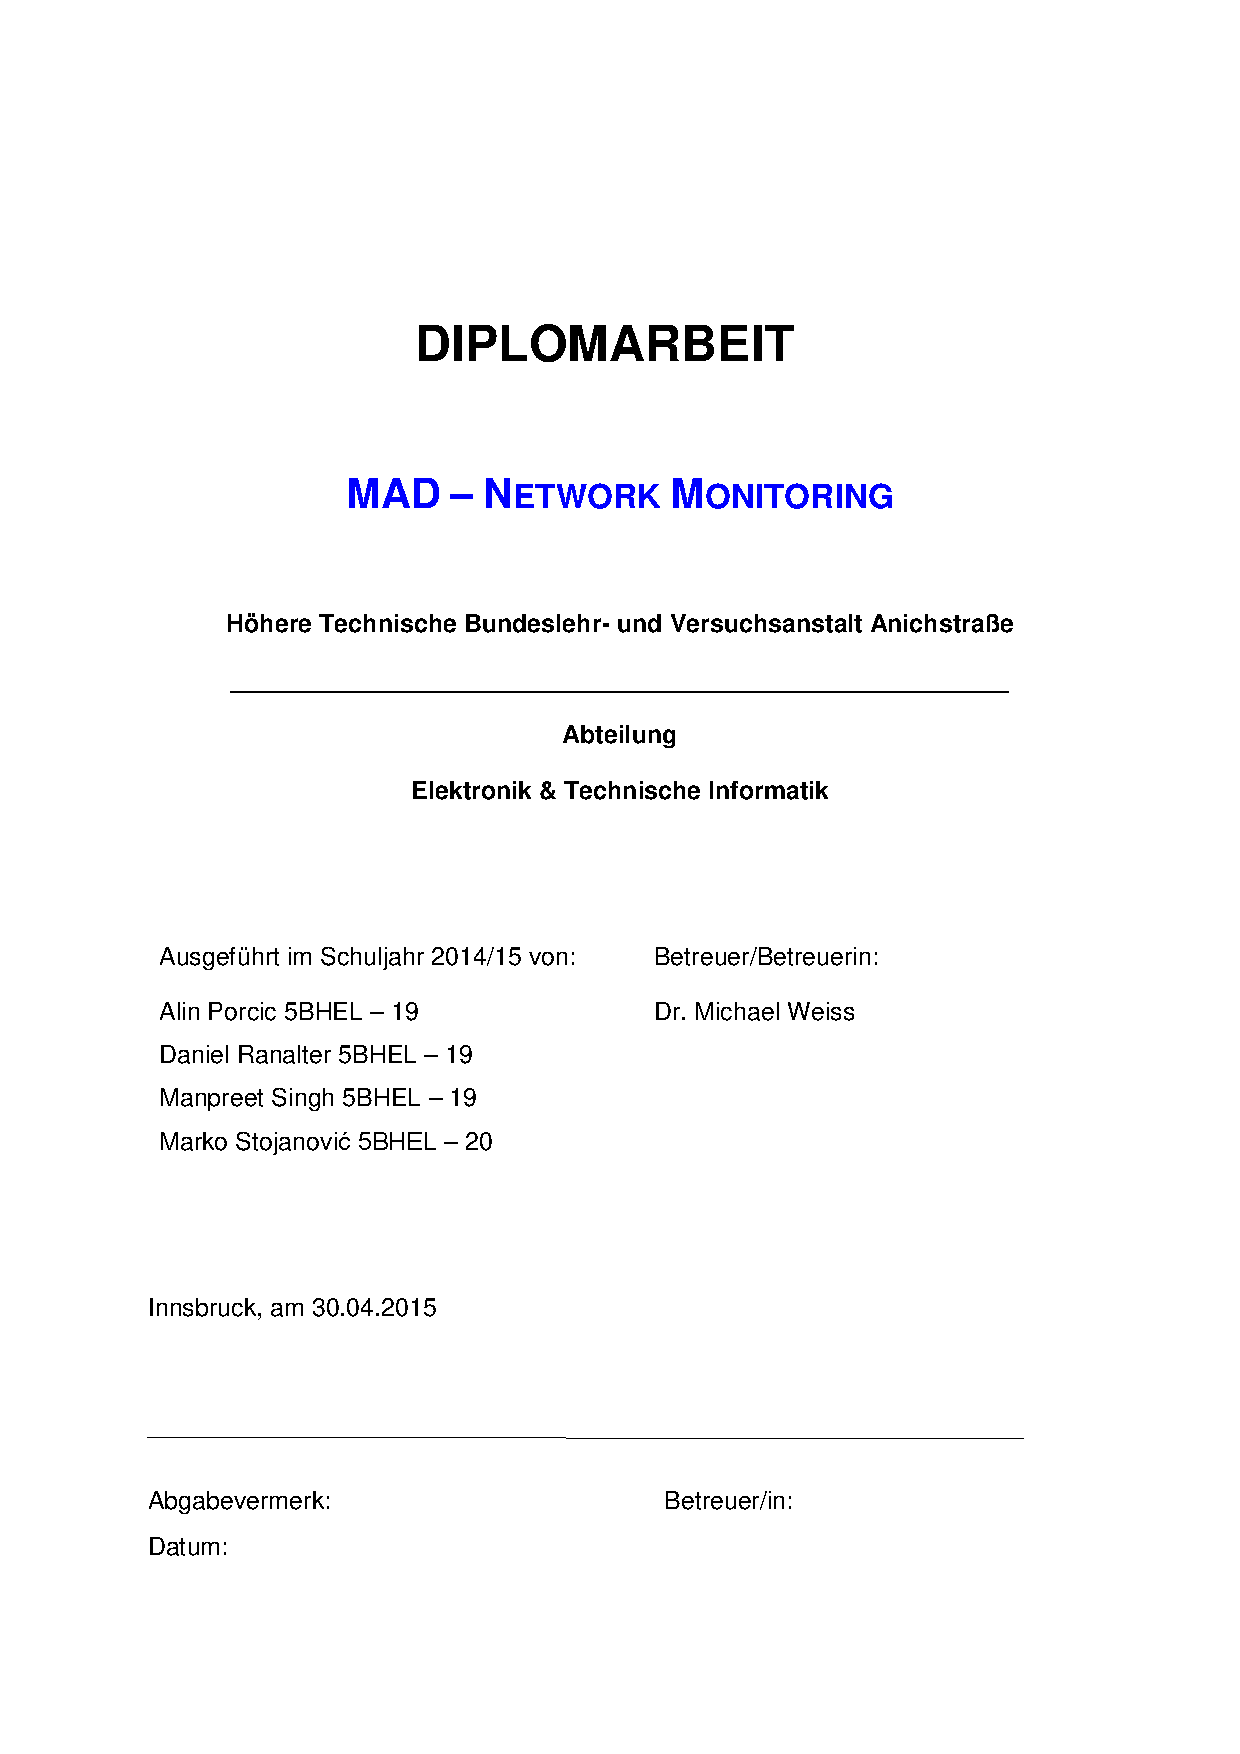
\includepdf[pages={1}]{../docs/general/Deckblatt.pdf}
\begin{onehalfspace}

\addcontentsline{toc}{chapter}{Vorwort}
\vspace{1.5cm}
\begin{Huge}
\textbf{Vorwort}
\end{Huge}
\vspace{2cm}
\\Mit dem Wachstum des Internets wird die Bedeutung von Netzwerken immer größer. Damit steigt auch die Notwendigkeit, durchgehend so gut wie möglich über den Zustand desselben informiert zu sein. Dies wird durch Monitoring bewerkstelligt, wessen Aufgabe es ist, das Netzwerk zu beobachten und den Admin über diverse Missstände zu informieren. Man kann zwischen zahlreichen kommerziellen und freien Lösungen wählen. Kommerzielle Lösungen sind jedoch überaus kostspielig und selbst die kostenlosen Varianten sind meistens bereits zuviel des Guten. 

Die damals anstehende Diplomarbeit, welche uns mit einer großen Herausforderung und wertvollen Erfahrungen lockte, sowie das bestehende Interesse in der Netzwerktechnik und der Programmierung waren der Anstoß für erste Gespräche innerhalb des Freundeskreises.Die zahlreichen Projekte, welche wir bereits gemeinsam bestritten, stimmten uns aufeinander ab. Zusammen mit der Freundschaft, die sich über die Jahre bildete, fiel es uns leicht, ein Team zu bilden.\\
Als Nächstes war es an uns, einen geeigneten Betreuer zu finden. Nach einigen Gesprächen und Überlegungen fiel die Entscheidung schlussendlich auf Prof. Dr. Weiss, welchen wir bereits im Jahr zuvor kennenlernten.\\
Als wir ihm bei einem ersten Gespräch unsere bisherigen Gedankengänge aufzeigten, entwickelte er mit uns zusammen schließlich die Idee, unsere Interessen zu kombinieren und ein Projekt zu entwerfen, dessen Aufgaben darin bestehen, ein Netzwerk zu überwachen.

\end{onehalfspace}
\begin{singlespace}
%\setcounter{tocdepth}{6}
\tableofcontents
\newpage
\end{singlespace}
\pagestyle{fancy}
\begin{onehalfspace}
\chapter{Abstract}
Mit den immer größer werdenden Anforderungen an die Netzwerktechnik ist es zur Herausforderung geworden, in einem Netzwerk den Überblick zu behalten. Große Firmen wie z.B. Cisco oder HP bieten Lösungen für dieses Problem, allerdings kosten die Produkte ein Vermögen. Es gibt auch einige kostenlose Produkte, wie z.B. Nagios. Die kostenlosen Varianten haben oft den Nachteil, dass die Konfiguration sehr komplex ist. Dadurch wird der Einsatz von Fachkräften nötig, und es entstehen auch hier hohe Kosten.
\paragraph{Problemstellung/Ziel:} Für das Überwachen von kleineren Netzwerken sind die oben genannten professionellen Lösungen nicht gut geeignet, da ihr Potential nicht annähernd ausgeschöpft wird. Unsere Diplomarbeit hat das Ziel, eine kompakte Lösung zu entwickeln, die kleine Netzwerke (max. 50 Netzwerkgeräte) überwachen kann. Gewünschte Funktionen sind zum Beispiel, das Scannen eines LANs oder das Überprüfen von Services. Außerdem soll diese Lösung auf Windows und Linux funktionsfähig sein.
\paragraph{Methodik:}Das Produkt Nagios ist uns ein erstes Vorbild gewesen. Unser prinzipieller Ansatz bestand darin, nur grundlegende Funktionen zu überwachen, wie z.B. einen HTTP-Dienst.
Die Wahl der Programmiersprache, fiel auf C\#, welche unter Windows auf das .net Framework und unter Linux auf Mono Framework aufbaut. Nachdem wir die Ziele definiert hatten, teilten wir das Projekt in mehrere Teilbereiche. Mit Hilfe des Versionsverwaltungsprogramms „Git“ war eine weitgehend reibungslose Zusammenarbeit möglich.
\paragraph{Resultat:} Das Ergebnis unserer Arbeiten ist ein Programm mit einem CLI (Command Line Interface), einem GUI (Graphical User Interface) und einer internen Datenverwaltung. Unser  LAN-Network-Monitoring stellt eine Lösung für grundlegende und kompakte Netzwerküberwachung dar. Es enthält verschiedene nützliche Funktionen (z.B. einen Portscanner) oder einige Dienstüberprüfungen (z.B. unseren HTTP-Checker). 
\chapter{Abstract (English)}
to be written

\chapter{Aufgabenstellung}

\section{Ziel}

Das Ziel dieser Diplomarbeit ist das Erstellen eines Programmes, welches in einem kleinen Netzwerk (max. 50 Netzwerkgeräte) Netzwerkgeräte und Netzwerkdienste überwachen kann. Dabei soll der Benutzer die Möglichkeit haben, Regeln für die Überwachung zu definieren, damit er bei einer Missachtung sofort per E-Mail darüber informiert werden kann.

\section{Schnittstellen}

Für die Benutzung des Programmes soll eine textbasierende Schnittstelle eingebaut werden, die die primäre Interaktion mit dem Programm sicherstellen soll. Die vollständige Überwachung sowie die Konfiguration aller Aufgaben und Geräte soll über diese Schnittstelle möglich sein.\\
Die Überwachung und die Konfiguration der Geräte und Aufgaben soll hauptsächlich über diese Schnittstelle ermöglicht werden.
Es soll auch die Möglichkeit bestehen, die textbasierende Schnittstelle über das Netzwerk zu nutzen. Daher muss diese Schnittstelle als Netzwerkdienst realisiert werden und es wird eine Client-Software benötigt.\\
Neben der textbasierten Schnittstelle soll eine graphische Schnittstelle implementiert werden, die eine alternative Benutzung des Programmes ermöglichen soll. Der Funktionsumfang der graphischen Oberfläche beschränkt sich auf die Anzeige einer Übersicht der Aufgaben und Geräte.

\section{Andere Voraussetzungen}

Das Programm soll auf Windows als auch auf Linux funktionstüchtig sein und die Benutzung soll sich auf den zwei verschiedenen Betriebssystemen nicht unterscheiden.\\
Die Resulate der Überwachungen sollen in einer lokalen Datenbank abgespeichert werden und es soll die Möglichkeit geben, die Datensätze der Datenbank zusammenzufassen, damit der Speicherbedarf der Datenbank reduziert werden kann.\\
Zudem soll das Programm bei Änderungen der IP-Adressen von Netzwerkgeräten informiert werden, damit dieser die neuen IP-Adressen nachtragen kann.

\part{Theorie zu den einzelnen Gebieten der Arbeit}

\chapter{Informatik (Marko Stojanovi\'{c})}
\lfoot{Marko Stojanovi\'{c}}

Die Informatik ist eine Wissenschaft, die sich mit der systematischen Verarbeitung von Informationen, speziell mit der automatischen Verarbeitung durch Digitalrechner, beschäftigt. Die Informatik ist aus der Mathematik und Ingenieursdisziplin (orientiert nach automatisch angewendeten Berechnungen) entstanden. [401]

\section{Programmiersprachen}

\subsection{Definition von einer Programmiersprache}
Bei einer Programmiersprache handelt es sich um eine formale Sprache, mit welcher Datenstrukturen und Algorithmen formuliert bzw. erstellt und ausgeführt werden können. Datenstrukturen und Algorithmen sind definierte Rechenvorschriften, welche sich durch Anweisungen nach bestimmten Mustern (Syntax) erstellen lassen. [402]\\
% http://de.wikipedia.org/wiki/Programmiersprache

Da Programmiersprachen künstlich erschaffene Sprachen sind, müssen beim Erstellen eines Programms eindeutige Algorithmen bestimmt werden, um eine korrekte Funktionalität gewährleisten zu können.\\
Um dies zu erreichen muss folgendes einer Programmiersprache definiert sein:

\begin{itemize}
\item Lexik\\
Die Lexik einer Programmiersprache ist mit der Rechtschreibung oder dem Vokabular einer Sprache gleichzustellen.\\
z.B.: Bei der Deklaration von Variablen in den Programmiersprachen PHP und Java. In der Programmiersprache PHP wird mit einem Befehl (var) eine Variable deklariert, die Typenzuweisung erfolgt automatisch. Bei Java muss immer der Datentyp der Variable korrekt zugewiesen werden. [402][403]
% [Was hat die Rechtschreibung bzw. Vokabular mit der Typenzuweisung zu tun?! Es ist ein unterschied, aber hat nichts mit der Lexik zu tun.]
\item Syntax\\
Die Syntax einer Programmiersprache ist mit der Grammatik einer natürlichen Sprach gleichzustellen (Sprachregeln).
Die Syntax einer Programmiersprache bestimmt die Reihenfolge bzw. das Muster der Befehle und macht es dadurch möglich, ganze "{}Sätze"{} zu schreiben. Zur Übersicht werden Syntaxdiagramme erstellt. [402]
\item Semantik\\
Die Semantik einer Programmiersprache bestimmt die Ereignisse, die eintreten nachdem eine syntaktisch richtige Aufforderung ausgeführt wird. [402]
\item Pragmatik\\
Die Pragmatik einer Programmiersprache bestimmt den Einsatzbereich, damit werden Probleme gezeigt, für welche die Programmiersprache eine gute Lösung bietet. [402]
\end{itemize}

\subsubsection{Minimalanforderungen an Programmiersprachen}
Programmiersprachen bieten viele Möglichkeiten an, folgende Eigenschaften zählen zu den Minimalanforderungen an Programmiersprachen:
\begin{itemize}
\item Ein- und Ausgabebefehle\\
Auf diese Weise wird eine Eingabe und Ausgabe von Daten realisiert.
\item Deklarationen\\
Variablen und Felder werden deklariert, damit Daten (Informationen) gespeichert oder nur zwischengespeichert werden können.
\item Grund- und Standardfunktionen der Mathematik\\
Mathematische Funktionen sind erforderlich, um programmieren zu können.
\item Grundfunktionen der Zeichenkettenverarbeitung\\
Dies ist für die Ordnung von belangen.
\item Steueranweisungen\\
Steuerung von (dauerhaften) Wiederholungen, eingeschränkten Ausführungen und Programmtrennung durch Unterfunktionen oder das Einbinden von Libraries. Höhere Funktionen lassen sich oft aus den vorhandenen Grundfunktionen erstellen und als Bibliothek einbinden. Auf diese Weise können viele problemorientierte (Spezial-) Sprachen erstellt werden. Softwareportabilität und die Effizienz der Programmierer wurde dadurch gesteigert.\\
Die Nachteile sind, dass es zu Geschwindigkeitsverlusten bei der Verarbeitung kommt und dem Programmierer werden vorhergesehene Lösungswege der verwendeten Spezialsprache aufgezwungen.
\end{itemize}
Programmiersprachen erreichen verschiedene Erfolge. Viele werden erfolgreicher und werden immer öfter verwendet,  Mehrzwecksprachen (Programmiersprachen, welche für verschiedene Anwendungen verwendet werden können) konnten mehrfach nur kleine Erfolge feststellen. [404]

\subsection{Wichtige Begriffe}
\subsubsection{Quelltext}
Als Quelltext (Quellcode) wird der Text bezeichnet, welcher die Anweisungen des Programmierers enthält. Diese Anweisungen müssen für die jeweilige Programmiersprache den Regeln entsprechend geschrieben werden. Bevor dieser Code ausgeführt werden kann muss er zuerst in eine Maschinensprache übersetzt werden. Eine Maschinensprache ist für den Menschen schwer verständlich, da sie im Binärcode geschrieben ist. [405]

\subsubsection{Compiler}
Als Compiler wird eine Software genannt, welche den Quellcode einer höheren Programmiersprache in eine Maschinensprache übersetzt, da die Ausführung ansonsten nicht möglich ist. Für jeden Prozessor (bzw. jede Prozessorfamilie) gibt es eigene Compiler. Ein Prozessor kann einen Compiler verwenden, solange dieser bei einem anderen Prozessor in der gleichen Prozessorfamilie verwendet wird und auch nur solange die Befehle kompatibel sind. Bei einer neuen Prozessorversion kann der alte Compiler immer noch verwendet werden, auch wenn neue Maschinen-Befehle integriert werden, Programmierer dürfen diese nur im Code nicht verwenden. Dies kann bei Pentium III-Prozessor und IV-Prozessor ausgenutzt werden.\\
Ein ausführbares Programm wird mit der Endung am Dateinamen "{}.exe"{} gekennzeichnet. Die Abkürzung ist englischer Abstammung (von "{}executable"{}).\\
Falls es sich um keine einfachen Compiler handelt, können Zwischenergebnisse entstehen.
Zwischenergebnisse werden von Compilern (oder anderen Übersetzungsvorgängen) in "{}.obj"{} Dateien abgelegt. Bei dem Zwischenergebnis handelt es sich um Maschinencode, welcher für die jeweilige Architektur übersetzt wurde. Im Objektcode ist normalerweise vorgeparsten Code und verwendete Programmbibliotheken.\\
Das genaue Format hängt von Compiler, Programmiersprache und der benutzten Maschine ab.
Nach Erstellung der Objektcodes folgt üblicherweise das "{}Linken"{}, durch welches das ausführbare Programm geliefert wird. [406]

\subsubsection{Interpreter}
Es handelt sich wieder um eine Software, welche den Quellcode einer höheren Programmiersprache in eine Maschinensprache übersetzt. Der große Unterschied ist, dass ein Compiler den Quellcode einmal in eine Maschinensprache umwandelt, um eine ausführbare Datei zu generieren. Bei einem Interpreter wird der Quellcode zeilenweise abgearbeitet, gegenwärtige Zeilen umgewandelt und die Befehle werden anschließend ausgeführt.\\
Interpreter werden zur Zeit hauptsächlich in Kombination mit Compilern verwendet.\\
z.B.: Bei Java wird der Quellcode vom Compiler in einen Byte-Code (Zwischencode, unabhängig von realer Hardware) umgewandelt und dieser wird während der Laufzeit der Software von einem Interpreter in Maschinensprache übersetzt, bei Java als "{}Virtual Machine"{} bezeichnet. [406]

\subsubsection{Linker}
Es kommt oft vor, dass Software-Produkte aus vielen verschiedenen und getrennt kompilierten Übersetzungseinheiten bestehen. Beim Übersetzen solcher Software entsteht eine Zwischendatei (Zwischenprodukt), welche auch als Objektdateien bezeichnet werden. Zwischendateien sind großteils in ausführbare Zielsprachen umgewandelt. Trotzdem sind sie nicht ausführbar, weil Programmteile, welche an anderen Orten erstellt wurden, fehlen. Das Format entspricht den Vorgaben des Zielsystems nicht.
\\Über einen Verbinder, den sogenannten Linker, werden die Zwischenprodukte zu einem ausführbaren Programm zusammengeschlossen. [406]

\subsubsection{Header-Dateien}
Allgemeine Deklarationsverwendungen von Bibliotheken sind in einer Header-Datei enthalten.
\\Funktionen, wie zum Beispiel "{}cin"{} und "{}cout{}", sind keine integrierten Bestandteile der verwendeten Programmiersprachen (z.B.: C++), wie im Gegensatz die Befehle "{}if "{} oder "{}else "{}. Funktionen, welche keine Bestandteile der Programmiersprache sind, können mit der Anweisung "{}\# include \textless stdio.h\textgreater "{} (eine Header-Datei namens "{}stdio.h "{}) eingekapselt werden. Dadurch wird gewährleistet, dass der Präprozessor (auch Präcompiler, ein Programm, welches vor der Übersetzung durch den Compiler wirksam ist) den Quelltext nach Zeilen kontrolliert, welche mit "{}\#"{} anfangen und Zeile, welche mit dem Inhalt der Header-Datei ersetzt. [406]

\subsubsection{Libraries}
Mit Libraries werden Sammlungen (Bibliotheken) von Programmfunktionalitäten, für passende Aufgaben, bezeichnet. Dabei handelt es sich um Hilfsmodule (keine eingeständige Einheit) für Programme.\\
In der Programmiersprache C++ enthält die Library namens "{}stdio.lib"{} die Funktion zur Ein- und Ausgabe von Daten auf dem Bildschirm ("{}cin"{} und "{}cout "{}).\\
Dabei muss auch zwischen Static und Dynamic Libraries unterschieden werden.

\begin{itemize}
\item Static Libraries\\
Funktionen, welche im Quellcode nicht angeführt sind, werden durch den Linker aus den benötigten Bibliotheken gesucht und im Programmcode ergänzt(auch bei Dynamic Libraries).
\\Von statischen Bibliotheken spricht man, wenn durch die Applikation der Umfang und der Speicherbedarf vergrößert werden.
\item Dynamic Libraries\\
Diese Art von Bibliotheken sind bei Multitasking-Systemen, die alle auf die gleichen Bibliotheken zugreifen, sinnvoll zu verwenden. Wenn zur Laufzeit eine bestimmte Funktion benötigt wird, wird diese von einem "{}Loader"{} im Arbeitsspeicher gesucht, wenn diese dort nicht gefunden wird, wird sie in den Arbeitsspeicher geladen.
\\Wird diese Funktion nun von einem weiteren Prozess angefordert, wird nur eine Verknüpfung an die entsprechende Stelle im Arbeitsspeicher erstellt.\\

Bei Verwendung von statischen Bibliotheken, wäre die von mehreren Prozessen verlangte Funktion für jeden Prozess in den Arbeitsspeicher geladen worden.\\

Dadurch wird die Ausführungszeit bei Programmen mit dynamischen Bibliotheken etwas verlängert, dies betrifft in erster Linie die Startzeit. Dennoch wird es akzeptiert, weil der gleiche Code der Bibliotheken, von allen Prozessen verwendet wird und dadurch der Speicherbedarf aller Programme geringer ist.
\\Dynamische Bibliotheken werden unterschiedlich unter den Betriebssystemen bezeichnet.
\begin{itemize}
\item Windows: dynamic link library ("{}dll"{})
\item Unix/Linux: shared library ("{}so"{} ... "{}shared object"{})
\end{itemize}
\end{itemize}
[406]

\subsection{Arten von Programmiersprachen}
\subsubsection{Höhere Programmiersprache} 
Von einer höheren Programmiersprache ist die Syntax nicht von der Hardware abhängig und ist an menschliche Bedürfnisse angepasst. Dadurch wird das Programmieren erleichtert, da eine Übersicht und Lesbarkeit geschaffen wird. [407]

\subsubsection{Maschinensprache}
Es handelt sich um eine Sprache aus Befehlen im Binärcode, welche für das Verständnis des Prozessors benötigt wird. Diese Sprache ist für die jeweilige Hardware ausgelegt und nicht für den Menschen, da sie nicht direkt lesbar ist. [407]

\subsubsection{Assembler}
Mit Assembler-Sprachen werden Sprachen bezeichnet, welche maschinennahe sind. Maschinennahe Sprachen sind auch sehr an die Hardware (Prozessor) angepasst.\\
Die Übersetzung eines Quellcodes in eine Maschinensprache erfolgt durch einen Assembler. Ein Assambler ist eigentlich ein Compiler, mit dem Unterschied, dass es beim Assambler für fast jede Assembleranweisung eine angenehme Darstellung gibt.
\\Zum Beispiel kann für 000001011110100000000011 der Befehl "{}add ax,1000"{} verwendet werden.\\
\\Diese Sprache ist bei zeitkritischen Anwendungen sinnvoll. [407]

\subsubsection{Skriptsprachen}
Skriptsprachen sind für kleine Anwendungen vorgesehen und in den meisten Fällen wird für die Ausführung ein Interpreter verwendet.\\
Um Programme schneller zu erstellen, wird bei Skriptsprachen auf einige Sprachelemente verzichtet, wie zum Beispiel auf Deklarationen von Variablen. Dies ist jedoch nur bei kleinen Programmen von Vorteil, bei großen wird dadurch die Fehlersuche erheblich erschwert.\\
Software, deren Quelltext in einer Skriptsprache geschrieben ist, wird als Skript (Scripts) bezeichnet. Microsoft nennt diese im Betriebssystemumfeld Makros.\\
Die Auslieferung von Scripts erfolgt meistens im Quellcodeformat, weil die Anpassung und Änderung von Programmen dadurch erleichtert wird.
\\Häufige Merkmale:
\begin{itemize}
\item implizite Deklaration von Variablen, dynamische Funktionsnamen
\item dynamische Typisierung
\item Speicherverwaltung, insbesondere Speicherbereinigung automatisch
\item Dynamik der Klassenzugehörigkeit oder prototypenbasierte Vererbung
\item Interpreter zur Ausführung des Quellcodes als eine Übersetzungsphase
\item Flexibilität der Sprache durch die Möglichkeit des Programms Manipulationen an sich selbst und anderen Dateien durchzuführen
\end{itemize}
Durch die Überschneidung von Compiler- und Skriptsprachen in den Anwendungsgebieten und ihren jeweiligen Eingenschaften, ist eine genau Unterscheidung nur schwer ersichtlich. [408]

\subsection{Programmierparadigmen}
Bei einem Programmierparadigma handelt es sich um einen elementaren Programmierstil, welcher den Prinzipien der einzelnen Programmiersprachen unterliegt. Die Prinzipien sind als Unterstützung, beim Programmieren von effizientem Code, gedacht.
\\Manchmal wird ein Lösungsweg dabei erzwungen.\\

Die Unterscheidung findet durch die jeweiligen Repräsentationskonzepte von dynamischen und statischen Programmelementen statt.
\begin{itemize}
\item dynamische Programmelemente\\
z.B.: Kontrollfluss, Datenfluss, Zuweisungen, ...
\item statische Programmelemente\\
z.B.: Konstanten, Variablen, Objekte, Methoden, ...
\end{itemize}
Programmiersprachen können verschiedene Programmierstile unterstützen, da sich die Programmierparadigmen auf verschiedene Anwendungssoftware beziehen und es sich nicht um abwechselnde Programmierstile handelt. [409]

\subsubsection{Strukturierte Programmierung}
Dieser Programmierstil wurde in den 1970er Jahren beliebt, als zum ersten Mal die Preise von Software höher waren als die von Hardware. Durch das strukturierte Programmieren konnten Programme in Prozeduren (Teilprogramme, Unterprogramme) zerlegt werden. Des Weiteren werden auf der untersten Ebene nur drei Kontrollstrukturen zur Begrenzung eingesetzt.
\begin{itemize}
\item Sequenz (nacheinander auszuführende Programmanweisungen)
\item Selektion/ Auswahl (bzw. Verzweigungen)
\item Iteration/ Wiederholungen (Schleifen)
\end{itemize}
Beim strukturierten Programmieren wird die umstrittene Sprunganweisung (GOTO), je nach Programmiersprache stark beschränkt. Wegen der beständigen Implementierung von Kontrollstrukturen und Prozeduren werden Codewiederholungen vermieden. Dadurch sind Quelltexte übersichtlicher und kürzer, damit wird die Fehlersuche erleichtert.\\

In allen Gebieten, in denen professionelle Programme entwickelt werden, ist die strukturierte Programmierung vorzufinden. Sie dient auch als Basis für neue Programmierparadigmen. Zu diesen gehören, die generative Programmierung, objektorientierte Programmierung und aspektorientierte Programmierung.
\\Strukturierte Programmierung ist mit folgenden Programmiersprachen auch mögliche:
\begin{itemize}
\item Ada
\item Algol
\item C und C++
\item COBOL (erst ab Fortran 77)
\item Java
\item Pascal, Modula- 2 und Oberon
\item Visual Basic
\end{itemize}
[410]
\subsubsection{Imperative Programmierung}
Die Bezeichnung kommt aus dem lateinischen und bedeutet anordnen. Auf diese Weise funktioniert auch dieser Programmierstil. Am Beginn des Quellcodes wird angegeben in welcher Reihenfolge die Anweisungen auszuführen sind.\\

Es ist das älteste Programmierparadigma. Die Entstehung ist durch die Größe älterer Programmiersprachen zustande gekommen. Es war die, zu dieser Zeit, klassische Programmierart. Sie bildet die Basis für einige Programmiersprachen, wie z. B.:
\begin{itemize}
\item ALGOL
\item Fortran
\item Pascal
\item Ada
\item PL/ I
\item Cobol
\item C
\item sämtliche Assemblersprachen
\end{itemize}
Die imperative Programmierung wird auch als "{}imperativ/ prozedural"{}, "{}algorithmisch"{} und "{}zustandsorientiert"{} bezeichnet. Ein häufig verwendeter Name ist auch "{}prozedurale Programmierung"{}, dieser ist jedoch falsch, weil es sich um ein Programmierparadigma mit anderen Definitionen handelt. [411]

\subsubsection{Deklarative Programmierung}
Dieses Programmierparadigma beschäftigt sich mit der Problemstellung, nicht nach der Lösung. Das Ziel ist es das Problem zu beschreiben und nicht wie beim imperativen Programmieren einen Lösungsweg zu entwickeln.
Folgende Sprachen stehen zur deklarativen Programmierung zur Verfügung:
\begin{itemize}
\item Haskell
\item Lisp
\item Prolog
\item XAML
\item im weiteren Sinne: SQL und XSLT
\end{itemize} 
Die deutlichen Unterschiede sind spätestens beim Entwickeln eines Algorithmus erkennbar, welcher aus Steuer- und Arbeitsmechanismus zu erkennen ist.\\

Durch die deklarative Programmierung sind diese Abteilungen voneinander getrennt. Bei imperativer Programmierung ist eine Trennung fast unmöglich, da Anweisungen an die Maschine programmiert werden. [412]

\subsubsection{Objektorientierte Programmierung}
Bei der objektorientierten Programmierung handelt es sich um einen Programmierstil, welchen die Programmstruktur durch einen eigenen Datentyp, dem sogenannten Objekt, unterstützt.\\

Es gibt auch eigene objektorientierte Sprachen (Smalltalk), die nach dem Grundsatz "{}Alles ist ein Objekt"{} funktionieren. Klassen, Typen (z.B. Integer) werden als Objekte betrachtet. Zu den bekanntesten objektorientierten Sprachen gehören:
\begin{itemize}
\item C\#
\item C++
\item Java
\end{itemize}
Die Prinzipien der Objektorientierung werden nicht von allen Sprachen gleich eingehalten. Bei den drei erwähnten Sprachen wird aufgrund dessen, dass Methoden und Strukturen nicht verwendet werden, elementare Datentypen als keine reinen Objekte zu betrachten. Die Einkapselung der objektorientierten Daten ist dem Programmierer frei überlassen.\\

Die erste objektorientierte Programmiersprache war Common Lisp/ CLOS mit dem ANSI/ X3.226-1994- Standard. Nach dem internationalen ISO- Standard wurde Ada 95 die erste objektorientierte Programmiersprache.
Simula- 67 war die erste berühmte objektorientierte Programmiersprache. Die Kapselung wurde anschließend in eine Klassenhierarchie und später in Smalltalk erweitert.\\

Programmiersprachen, die heute verwendet werden, wie Python, unterstützen das Konzept des prozeduralen und objektorientierten Ansatzes. Das prozedurale Konzept wurde in den 1970er und 80er Jahren von Pascal, Fortran und C verwendet. Die älteste objektorientierte Programmiersprache ist Smalltalk, welche heute auch noch von Bedeutung ist. Viele objektorientierte Programmiersprachen sind aufgrund von Smalltalk entstanden, konnten jedoch keine Erfolge bringen, weil die Implementierungen zu teuer waren.\\

Die objektorientierte Programmierung konnte den Durchbruch erst in den 1990er Jahren feiern. In den 1960er Jahren wurde, aber Simula- 67 zur Entwicklung von Lösung für Modularisierung und Code- Wiederverwendbarkeit verwendet.\\
\\In Self, JavaScript und NewtonScript gibt es keine Klassendeklarationen, weil neue Objekte durch bereits vorhandene Objekte abgeleitet werden (sogenannte "{}Prototypen"{}). Verwendung von Methoden und Attributen eines Prototyps finden dann statt, wenn es im neuen (abgeleiteten) Objekt keine genaue Anweisung zur Überschreibung gibt. Dadurch ist man schneller beim Erstellen, was sich bei bei der Programmierung kleiner Anwendungen lohnt.\\

In anderen objektorientierten Sprachen (z.B. Objective C) sind sogenannte Klassenobjekte vorhanden. Klassenobjekte gibt es für jede Klasse und repräsentieren die jeweiligen Klassen während der Ausführung und sind für die Erzeugung von Objekten der Klasse und für Methodenaufrufe verantwortlich.\\

Klassenbibliotheken fassen normalerweise Klassen zusammen. Oft sind sie thematisch organisiert. Dadurch können Klassenbibliotheken implementiert werden, welche verschiedene Möglichkeiten mit sich bringen, z.B. den Datenbankzugriff. [413]

\subsection{Visual C\#} 
Das Ziel von C\# ist es schnelle und einfache Lösung zur Erzeugung von .NET-Anwendungen zur Verfügung zu stellen. Dazu gehören auch Webdienste und ASP.NET-Webanwendungen. In C\# programmierte Programme basieren auf Diensten der Common Language Runtime, hinzukommt die komplette Nutzung aller Vorteile welche von .NET Framework ermöglicht werden. Es ist eine von Microsoft neue, einfache, professionelle und objektorientierte Sprache, welche in vielen Anwendungen einen Einsatz finden kann.\\

C\# wird von allen leicht zu erlernen sein, die bereits C oder identische Programmiersprachen kennengelernt haben, da mit C\# eine rasche Entwicklung angeboten wird, ohne auf die Stärken und die Sicherheit von C und C++ zu verzichten.\\

Es werden systeminterne Mechanismen für geheimen Code bereitgestellt, welche hohe Standards an Sicherheit, Garbage Collection und Typ-Sicherheit garantieren.
\\Auch eine einfache Vererbung wird zur Verfügung gestellt. Durch die bereits vorhandene .NET Framework und Common Language Runtime werden Garbage Collection, Sprachinteroperabilität, weiterentwickelte Sicherheitskonzept und Versions-Kontrollen angeboten.

Es wurden Namespaces, Klassen, Enumerationen, Überladen und die strukturierte Ausnahmebehandlung vereinfacht und auf den neuesten Stand gebracht. Makros, Mehrfachvererbung und virtuelle Basisklassen sind Fähigkeiten von C und C++, welche entfernt wurden. Durch C\# steht eine leistungsfähige und produktive Programmiersprache als Ersatz für C und C++ zur Verfügung.
\\Folgende übliche Projekttypen können verwendet werden:
\begin{itemize}
\item Klassenbibliotheken
\item Windows- Steuerelementbibliotheken
\item ASP.NET- Webanwendungen und -Webdienste
\item Web- Steuerelementbibliothek
\item Windows-Dienste
\item Konsolenanwendungen usw.
\end{itemize}
[414]
\subsubsection{Wichtige Eigenschaften von C\#}
Wie bereits erwähnt handelt es um eine elegante, typsichere und objektorientierte Sprache, die zur Entwicklung sicherer und resistenter, in .NET Framework ausgeführter Software verwendet werden kann. Es können Anwendungen im breiten Spektrum erstellt werden, wie z.B.: Windows- Clientanwendungen, XML- Webdienste, Client- /Serveranwendungen, Anwendungen für Datenbanken, ...\\

Auf Grundlage der C\# - Sprache und .NET Framework wird von Visual C\# ein Code- Editor mit angenehmer Benutzeroberfläche, eingebauten Debugger und anderen Hilfsmitteln zur Verfügung gestellt.\\

Die Programmiersprache ermöglicht auch die Nutzung von produktiven Fähigkeiten.
\\Zu diesen zählen:
\begin{itemize}
\item festlegbare Werttypen auf NULL
\item Enumerationen
\item Delegaten
\item Lambda- Ausdrücke und direkter Speicherzugriff (in Java nicht enthalten)
\item Unterstützung generischer Methoden und Typen\\
Dadurch wird eine Optimierung der Typsicherheit, Leistung und Iteratoren (Entwurfsmuster) erzielt. Durch die Einbindung von Auflistungsklassen können benutzerdefinierte Entwurfsmuster definiert werden. Der Zugriff vom Clientcode erfolgt problemlos.
\item Language- Integrated Query (LINQ)\\
Integrierte Abfrage-Ausdrücke bewirken Abfragen mit starker Typisierung. Es sind Abfragefunktionen für verschiedenste Datenquellen eingebaut.
\item Objektorientierung\\
Kapselung, Vererbung und Polymorphie wird ermöglicht.
\item direktes Erben von übergeordneten Klassen möglich
\item Implementierung beliebiger Schnittstellen
\item Überschreibung virtueller Methoden\\
Zum Schutz von unbeabsichtigten Neudefinitionen ist das Schlüsselwort "{}override"{} beim Überschreiben von virtuellen Methoden in übergeordneten Klassen zu verwenden.
\item  Strukturen
\begin{itemize}
\item auf einem Stapel reservierter Typ
\item Schnittstellen implementierbar
\item keine Vererbungen
\item identisch einer vereinfachten Klasse
\end{itemize}
\item gekapselte Methodensignaturen\\
Sie werden auch als "{}Delegaten"{} bezeichnet und stellen Ereignisbenachrichtigungen zur Verfügung.
\item Accessoren für private Membervariablen
\item Erstellung deklarativer Metadaten zu Typen während der Laufzeit
\item Inline-XML-Dokumentationskommentare
\item Durch Interupt (Prozess) wird eine Kommunikation mit Windows- Programmen (z.B.: COM- Objekte, systemeigene Win32-DLLs) aufgebaut.
\item Zeiger-Unterstützung
\item keine Separation der Header-Dateien
\item keine einzuhaltende Ordnung der Deklaration von Methoden und Typen
\item Definitionen von Klassen, Strukturen, Schnittstellen und Ereignissen kann nach Belieben definiert werden.
\end{itemize}
[415]

\subsubsection{.NET Framework}
Die Ausführung, von in C\# erstellten Programmen, erfolgt auf Grundlage von .NET Framework. Es handelt sich dabei um eine integrale Komponente von Windows. Die Komponente besitzt eine Common Language Runtime (CLR) und einen zusammenhängenden Klassenbibliotheken- Satz. Bei der CLR handelt es sich um ein virtuelles Ausführungssystem, welches eine Implementierung von Microsoft zur Common Language Infrastructure (CLI) ist.\\

CLI ist ein Standard, durch welchen die Basis für die Erstellung von Entwicklungs- und Ausführungsumgebung auf internationaler Ebene definiert ist. Nach den CLI- Vorschriften wird der C\# - Quellcode in einen IL- Code (Intermediate Language Code) kompiliert und es entsteht eine mit den Ressourcen (z.B.: Bitmaps, Zeichenfolgen) eingebundene Assembly (ausführbare Datei, Erweiterungen sind "{}.exe"{} oder "{}.dll"{} Dateien).\\

Zu jeder Assembly gibt es eine Manifest- Datei, welche Typen, Version, Kultur und Sicherheitsanforderungen enthält. Jede Kompilierung eines C\# - Programms bewirkt ein laden der Assembly in die CLR, dabei werden unterschiedliche Aktionen ausgeführt, diese werden durch den Inhalt der Manifest- Datei bestimmt. \\
\begin{itemize}
\item Sicherheitsanforderungen erfüllt\\
In diesem Fall werden durch die CLR der IL- Code mit der JIT- Kompilierung (Just- In- Time) Maschinenanweisungen generiert.
\item weitere Dienste der CLR
\begin{itemize}
\item automatische Garbage Collection
\item Ausnahmehandlungen
\item Ressourcenverwaltung
\end{itemize}
\item ausführliche Bibliothek
\begin{itemize}
\item 4 000 Klassen
\item breites Spektrum an Funktionen\\
Ein-/Ausgabe von Dateien, Zeichenfolgebearbeitung, XML- Analysen, Windows- Forms- Steuerelemente, ...
\item Routinearbeiten von C\# - Programmen werden größten Teils mit .NET Framework- Klassenbibliotheken erledigt
\end{itemize}
\end{itemize}
Zu den wichtigsten Eigenschaften von .NET Framework zählt die Sprachinteroperabilität.\\

Damit ist es möglich, dass der Code mit dem Code anderer Programmiersprachen, die mit Common Type Specificaion (CTS) kompatibel sind, gekapselt wird. Neben Visual Basic, Visual C++ gibt es noch viele weitere. Es können unterschiedliche .NET- Programmiersprachen zur Erstellung von Modulen für eine Assembly verwendet werden. Auch die Typen können einen Bezug aufeinander haben, trotz unterschiedlicher Programmiersprachen.
\begin{center}
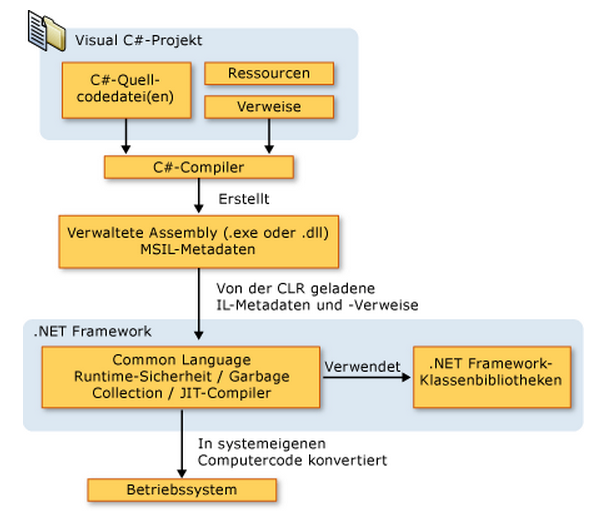
\includegraphics[scale=0.8]{img/uebersetzung.png}\\
Beziehung zwischen C\# - Quelltext, .NET Framework- Klassenbibliotheken, Assembly und der CLR (während der Kompilierungs- und Laufzeit).
\copyright Microsoft\\
Quelle: https://msdn.microsoft.com/de-de/library/z1zx9t92.aspx - 05.04.2015
\end{center}
[415]

\subsubsection{Vorteile von C\#}
Dies sind nur einige der zu erwähnenden Vorteile von C\# .
\begin{itemize}
\item einfache, typsichere, professionelle und objektorientierte Programmiersprache
\item Programme können zu den unterschiedlichsten Gebieten geschrieben werden
\item durch besondere Features sind dauerhafte Komponenten auf Systemebene möglich zu realisieren
\begin{itemize}
\item gesamte COM-/ Plattformunterstützung (Einbindung von existierendem Code)
\item Garbage Collection und Typsicherheit gewährleisten eine Stabilität
\item systemintegrierte Mechanismen für Codevertrauenswürdigkeit ergänzen die Sicherheit
\item entwicklungsmögliche Metadatenkonzepte werden vollkommen unterstützt
\item plattformübergreifende Verwendungsmöglichkeit ...
\end{itemize}
\end{itemize}
[416]
\section{Multithreading}
Prozesse müssen von Programmierern oft gut geplant werden, dabei muss oft über Threads nachgedacht werden, damit es zu keinen Fehlern im Programm kommt.\\

Unter Multithreading ist das "{}gleichzeitige"{} Abarbeiten, verschiedener Threads, von einem Prozess oder einem Anwendungsprogramm, zu verstehen. Multithreading wird auch als Nebenläufigkeit, Mehrsträngigkeit oder Mehrfädigkeit bezeichnet. [417]

\subsection{Threads}
Ein Thread (Programm-Faden) steht in der Informatik für einen Ausführungsstrang oder auch eine Ausführungsreihenfolge beim Abarbeiten eines Programms und ist ein Teil eines Prozesses. Threads werden auch Aktivitätsträger oder leicht gewichtete Prozesse genannt. Es gibt Kernel-Threads und User-Threads. [418]

\subsubsection{Kernel-Thread}
Aus der Sicht des Betriebssystems ist ein Thread ein sequentieller Abarbeitungslauf eines Prozesses. Dabei teilen sich alle, zu einem dazugehörenden Prozess, verschiedene Ressourcen. Zu diesen Ressourcen gehören: Codesegmente, Instantiierung des Datensegmentes mit gleichem Datenlayout und die verwendeten Dateideskriptoren im Datensegment. Von Friedrich L. Bauer wurde früher der Begriff "{}Sequentielle Prozesse{}" geprägt.\\

Threads, welche zu einem Prozess gehören, werden von verschiedenen Prozessoren ausgeführt, wenn mehrere Prozessoren vorhanden sind. Ist nur ein Prozessor vorhanden, werden voneinander unabhängige Registersätze und Stacks, welche verschiedenen Teilen des Adressraums zugeordnet sind, verwendet.\\

Alle Threads benutzen alle Betriebsmittel, bis auf jene welche nur von den erzeugenden Threads benutzt werden können oder dürfen. Da es zu Konflikten kommen kann, werden Synchronisationsmechnismen eingesetzt, um diese potentielle Gefahr zu umgehen.
Kommunikation zwischen allen Threads, die zu demselben Prozess gehören, ist möglich, da sie den gleichen Adressraum belegen. Das kann mit der Interprozesskommunikation bei Prozessen verglichen werden.\\

Threads von Programmfunktionen sind übersichtlich aufteilbar, da jeder für eine Aufgabe die Verantwortung trägt.  Je nach Betriebssystem können Threads verschiedene Zustände annehmen, bei dem Großteil sind es: 
\begin{itemize}
\item inaktiv -  Thread nicht gestartet
\item running (aktiv) - Befehl vom Thread wird auf der CPU ausgeführt
\item ready (bereit) - Thread ist gestoppt, um anderen Thread aktiv werden zu lassen
\item waiting (blockiert) - Thread wartet auf Ergebnis
\end{itemize}
[418]
\subsubsection{User-Thread}
In der Informatik versteht man unter einem User-Thread eine festgelegt Art Programme bzw. Programmteile verzahnt auszuführen. Die Funktionalität ist in einer separaten Programmbibliothek im Userspace implementiert. Auf diese Weise wird ein Kontextwechsel (Taskswitching) zwischen den User-Threads ohne komplizierte Systemaufrufe gewährleistet, dadurch sind diese auch schneller als Wechsel zwischen Kernelthreads oder Prozessen.\\
Ein User-Thread wird auch "{}Userlevel-Thread"{} bezeichnet und unter Windows als "{}Fiber"{}. [418]
%\subsubsection{Implementierung}

\subsubsection{Schwierigkeiten}
Synchronisationsmechanismen von Threads, wie Mutexen und Semaphoren sind in der Umsetzung anspruchsvoll, weil die Programmabläufe nicht nur sequentiell sind. Durch das Regeln eines Scheduler von Ausführungsreihenfolge und den Wechseln zwischen den Threads, auf welchen der Programmierer fast keinen Einfluss hat, ist eine richtige Vorhersage dadurch schwer zu ermitteln, ob ein parallel laufendes Programm, ohne großen Aufwand in ein unvorhergesehen Gesamtzustand geraten kann, der durch Deadlocks, Livelocks, Datenfehler und Abstürze ersichtlich wird.\\
Fehler dieser Art sind schwer reproduzierbar und die Fehlersuche ist schwierig. [418]

\subsection{Konzept von Multithreading}
Threads werden, im Gegensatz zu Programmen (Multitasking), nicht komplett von einander getrennt (gleichzeitig oder quasi gleichzeitig) ausgeführt. Dadurch kann es durch Race Conditions zu Fehlern kommen, welche durch Synchronisation vermieden werden.\\ 
In Echtzeit parallel laufende Ausführungen von Programmen und Threads können nur erreichen werden, wenn mehrere Prozessorkerne vorhanden sind und miteinander kommunizieren (Multiprocessing). [418]

\subsubsection{Hardwareseitiges Multithreading}
Der Unterschied zwischen hardwareseitigem und softwareseitigem Multithreading ist, dass softwareseitiges Multithreading nur aufgrund von Software gleichzeitig oder scheinbar gleichzeitig Threads ausführt und dadurch mehr Leistung in Anspruch nimmt. Beim hardwareseitigem  Multithreading wird die CPU durch die Hardware entlastet.\\

Prozessoren mit hardwareseitigem Multithreading können effektiver ausgelastet werden, da auf ihren Prozessorkernen mehrere Operationen zur gleichen Zeit ausführbar sind. Dadurch wird das parallele Ausführen von verschiedenen Threads ermöglicht. Bei der Ausführung auf einem Prozessor müssen sich Threads alle Betriebsmittel eines Prozessorkerns teilen.\\

Ein schneller Wechsel zwischen den Programmen wird durch den Einsatz von einem Registersatz mit Stapelspeicher und Programmzähler an jedem Thread gewährleistet. Dadurch sind Umschaltzeiten von 0,1-10us möglich, im Gegensatz zum Kontextwechsel des Betriebssystems, welches eine Zeit von 10-30ms benötigt.\\

In modernen Prozessoren wird versucht eine noch größere Auslastung des Prozessors zu erreichen, durch das Out-of-Order execution (eine Möglichkeit, um die Reihenfolge der Ausführungsinhalte von Maschinenbefehlen zu ändern). Dadurch wird die Pipeline ausgelastet. Tests haben ergeben, dass es dabei jedoch zu Pipeline-Hazards kommen kann.

Threads werden von multithreadingfähigen Prozessoren deswegen quasi-gleichzeitig verwendet. Dazu gibt es mehrere Möglichkeiten:
\begin{itemize}
\item time-slices: Durch einen Algorithmus ist definiert wie lange ein Thread ausgeführt wird, dadurch kann immer nur ein einziger Thread ausgeführt werden.
\item switch-by-event: Durch bestimmte Ereignisse kann es zum Wechsel kommen.
\item simultanes Multithreading (SMT): Ein Registerfile-Bereich wird für kleine Prozessorkontexte reserviert und ein Thread ausgeführt. Gleichzeitig laufende Threads benutzen damit das selbe Rechenwerk.
\item Core MultiThreading: Das gleichzeitige Ausführen mehrerer Threads wird dadurch ermöglicht, dass im Prozessor mehrere Arithmetisch-logische Einheiten (ALU) integriert sind, welche sich eine Gleitkommaeinheit teilen.
\end{itemize}
Heutzutage sind bei PCs DualCore, QuadCore oder HexaCore- Prozessoren zu finden. Diese sind mit zwei, vier oder sechs parallelen Pipelines ausgestattet. [419]


\subsubsection{Softwareseitiges Multithreading}
Softwareseitiges Multithreading wird oft in Verbindung mit nur einem Prozessor verwendet. Die vermeintlich gleichzeitige Abarbeitung wird durch Sequentialisierung, auch Thread-Priorisierung genannt, und durch ein verkleinertes Multiplexverfahren organisiert. Dadurch können einzelnen Threads von einem Task angeblich gleichzeitig arbeiten. Bei Videospielen kann dann z. B. der erste Thread eine Szene berechnen und der zweite Thread kann auf die Eingaben des Spielers warten und reagieren.\\

Die Gesamtleistung des Systems wird auch ohne zusätzliche Hardwareunterstützung durch den Overhead (wird beim Kontextwechsel gebildet) nur leicht beeinträchtigt. Nur wenn komplett voneinander getrennte Abläufe stattfinden, wird viel Leistung beansprucht.\\

Es ist auch abhängig ob eine Multithreading-Unterstützung, durch das Betriebssystem, auch geboten wird. Wenn nur in der Anwendung Multithreading implementiert ist, gibt es keine Beschränkungen für den Programmierer bei der Zuordnung von Threads und den dazugehörigen Ressourcen. Die ganze Anwendung kann vom Betriebssystem gestoppt werden, wenn Dienste und Ressourcen benötigt werden, diese jedoch nicht zur Verfügung stehen. Es handelt sich um das sogenannten "{}Primär Problem"{}, dass bei der Ausführung interner Daten Prozeduren auf grafischen Oberflächen vorzufinden ist. Das Programm kann nur weiter seine Dienste anbieten, wenn eine Multithreading-Unterstützung vom Betriebssystem vorliegt, weil dieses die belegten Ressourcen und Dienste kennt.\\

Von Threads gemeinsam verwendete Ressourcen eines Programms können sein: Adressraum, Datei- Handle, ... [420]
\newpage
\lfoot{Daniel Ranalter}
\chapter{Netzwerkgrundlagen und Protokolle (Daniel Ranalter)}
\lfoot{Daniel Ranalter}
Dieser Teil der Abhandlung wird die Netzwerkgrundlagen, die auf das Ethernet Protokoll (siehe Kapitel \ref{ssec:eth} auf Seite \pageref{ssec:eth}) aufsetzen, abdecken. Es gibt noch diverse andere, wie zum Beispiel Token Ring, auf welche hier im Folgenden jedoch nicht näher eingegangen wird, da, abgesehen davon, dass Ethernet auch bei der praktischen Durchführung verwendet wurde, Ethernet das am häufigsten genutzte Layer1 Protokoll darstellt. 

\section{Grundlagen}
In der Netzwerktechnik gibt es mehrere verschiedene grundlegende Konzepte, auf welche hier eingegangen werden soll.

\subsection*{Übersicht: Netzwerkdevices$^{[204]}$}
\addcontentsline{toc}{subsection}{Übersicht: Netzwerkdevices}
Um ein Netzwerk aufzubauen, werden verschiedene Devices benötigt. Je nach Größe und Art des Netzwerkes kann man auch auf einzelne Komponenten verzichten. 

\subsubsection{Router}
Ein \textbf{Router} kommt in so gut wie jedem Netzwerk vor. Er operiert auf dem \textbf{Layer 3} im OSI-Schichtenmodell, indem er Pakete, welche er von einem Netz bekommt, anhand der IP-Adresse an einem anderen Interface hinaus in ein anderes Netzwerk schickt. Dadurch verbindet er logisch getrennte Netze.\\

\begin{center}
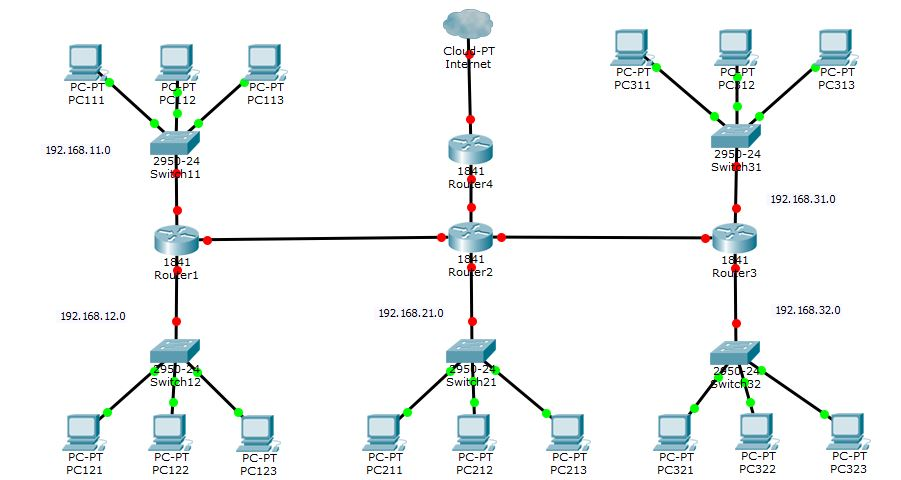
\includegraphics[scale=0.5]{../docs/tarkes/pics/RouterNetwork.jpg}\label{fig:bspNetwork}
\end{center}

Das Wissen, welches Paket wohin muss, zieht er aus einer \textbf{lokalen Routingtabelle}. Diese Tabelle kann auf drei unterschiedliche Arten entstehen:\\
\begin{itemize}
\item \textbf{Direkt angeschlossene Netze}\\
Netze, welche direkt an einem seiner eigenen Interfaces hängen, erkennt er ohne weiteres Zutun.\\
Auf dem Bild wären die Netze 192.168.11.0, 192.168.12.0 und 192.168.22.0 dem Router1 bekannt und er könnte Anfragen von Host121 an Host111 frei von jeglicher weiteren Konfigurierung weiterleiten.
\item \textbf{Statisches Routen}\\
Es ist dem Admin eines Netzwerkes möglich, alle möglichen Routen von einem Netz zum anderen händisch am Router einzutragen.\\
Vorteilhaft daran ist die hohe Sicherheit und Kontrolle über das Netzwerk, nachteilig jedoch, dass es bei größeren Netzwerken sehr schnell sehr schwer umsetzbar wird statisches routen anzuwenden, da es sehr viel Arbeit darstellt, jede mögliche Route händisch einzutragen ohne dabei einen Fehler zu begehen.\\
Anhand des Bildes wäre es dem Administrator des Netzwerkes zum Beispiel möglich Router1 zu sagen, dass, wenn er zu Host212 kommen will, über das Netz 192.168.22.0 gehen muss. Was danach passiert, braucht Router1 nicht zu wissen, da sich nun Router2 um das Paket kümmern muss. Er erkennt, dass die Ziel IP-Adresse sich in einem direkt angeschlossenen Netz befindet und schickt das Paket an dem entsprechenden Interface raus.
\item \textbf{Dynamisches Routen}\\
Beim dynamischen Routen lernt der Router anhand von eigenen Routing Protokollen wie er zu welchem Netz kommt. Die diversen Protokolle setzen verschiedenste, auf die jeweilige Situation abgestimmte, Prioritäten. So versucht das Protokoll OSPF (Open Shortest Path First) immer so wenig Hops, also Netzwerkwechsel/Router, wie möglich passieren zu müssen. RIP (Routing Information Protocol) und dessen Nachfolger RIP2 werden zwar noch verwendet, aber als veraltet angesehen.
\end{itemize}

%Dagegen muss was getan werden
%----
Des weiteren gibt es verschiedenste Arten von Routern. Ihre Grundfunktionalitäten sind zwar immer die gleichen, jedoch würde das kleine Kästchen, das zuhause steht, nie ausreichen, um den Traffic der Backboneleitungen, also der großen Glasfaserleitungen, welche die Kontinente verbinden, zu routen. Dafür würde diesem Router einfach die Leistung fehlen.\\
%----
Deshalb gibt es verschiedene Arten von Routern. Ein paar Wichtige sind:\\
\begin{itemize}
\item Backbone-Router\\
Hochgradig auf Datendurchsatz optimiert, werden sie, wie der Name schon sagt, für das Routen an der Backbone verwendet.
\item Edge-Router, Border-Router\\
Wird von ISPs verwendet, um die Netzwerke ihrer Clienten zu verbinden. Sie verwenden normalerweise das Routing Protokoll BGP (Border Gateway Protocol), welches für diese Aufgabe ausgelegt ist.
\item WLAN-Router\\
Im Grunde ganz normale Router, welche jedoch zusätzlich die Möglichkeit besitzen, nicht nur kabelgebunden zu kommunizieren, sondern auch über das Funkband. In Österreich sind die Bänder 2,4 GHz und 5 GHz in Verwendung.
\item Customer-Edge-Router\\
Werden meistens von den ISPs den Kunden zur Verfügung gestellt. Beinahe alle unterstützen heutzutage auch WLAN.
\end{itemize}
\subsubsection{Switch}
Ein \textbf{Switch} ermöglicht die Kommunikation zwischen mehreren Hosts. Einfache Switches agieren hauptsächlich auf dem \textbf{Layer2}: Sie speichern ab, an welchem Port welche MAC-Adresse hängt und wissen dann durch Source und Destination MAC-Adresse, an welchem Interface das Ziel des Paketes liegt\\

Im Gegensatz zu ihren Vorgängern, den \textbf{Hubs}, sind sie damit in der Lage, Pakete zielgerichtet weiter zu leiten. Hubs lenken einkommenden Traffic nicht, sie schicken die Pakete immer an alle Interfaces. Switches legen dazu eine \textbf{lokale Switching Tabelle} an, in welcher steht, an welchem Interface welche MAC-Adresse liegt.\\
Darin findet sich jedoch auch die größte Sicherheitslücke, wie später in Kapitel \ref{sec:security} auf Seite \pageref{sec:security} noch besprochen wird.\\

Switches trennen also auch keine Netze, sondern sorgen für Kommunikation innerhalb eines Netzes. So sieht man zum Beispiel im vorhergehenden Bild, dass die Switches, abgebildet als viereckige Kästchen, drei PCs zu einem Netzwerk zusammenfassen und mit dem Router verbinden.\\

Auch hier gibt es wieder verschiedene Ausführungen. Die wichtigsten sind die Standart Switches, welche auf Layer 2 agieren.\\
Als nächste große Gruppe gibt es die sogenannten Layer3 Switches. Diese, wie der Name bereits andeutet, verfügen über Funktionalitäten auf dem 3. Layer der OSI-Schicht. So sind sie in der Lage zu routen, was vor allem bei VLANs benötigt wird, oder auch die Priorisierung von bestimmten Paketen, um Quality of Service zu gewährleisten.\\
Es gibt auch noch Switches, welche höheren Layers zugeordnet werden Diese sind jedoch nicht einheitlich, sondern werden von Hersteller zu Hersteller unterschiedlich definiert.
\subsubsection{Firewall}
Die \textbf{Firewall} ist eine \textbf{Sonderform des Routers}.\\
Eigentlich ist die Firewall an sich nur eine Software, welche nach zugrunde liegenden Bestimmungen entscheidet, welche Pakete durch dürfen und welche nicht. Jedoch wird dies in großen Firmen häufig von einem dafür spezialisierten Router erledigt, welcher dann als Firewall bezeichnet wird.\\
Firewalls haben dann meistens nur 2 Ports, da ihre einzige Aufgabe ja darin besteht, Pakete zu blockieren oder durchzulassen. Dafür sind sie sehr stark auf ihren Datendurchsatz optimiert, da sie so gut wie immer den Flaschenhals eines Netzes darstellen.\\
Es gibt auch hier unterschiedliche Arten von Firewalls:\\
\begin{itemize}
\item \textbf{Packet Filters}\\
Packet Filters sind die primitivste Art von Firewalls. Sie entscheiden anhand der \textbf{Source- und Destination IP, Source- und Destination Port sowie UDP/TCP Parameter}, ob ein Paket als vertrauenswürdig eingestuft wird oder nicht.
\item \textbf{Stateful Inspection}\\
Dies stellt eine Erweiterung zu dem Packet Filter dar. Die Firewall speichert nun auch den \textbf{State}, also den Zustand eines Paketes oder einer Kommunikation. So kann man der Firewall zum Beispiel sagen, dass Pakete, welche zu einer bestehenden Kommunikation gehören, durchgelassen werden dürfen. 
\item \textbf{Application Level Firewall}\\
Der Vorteil dieser Art an Firewall ist, dass sie in der Lage ist, bestimmte Protokolle und Anwendungen zu \glqq verstehen\grqq . Das bietet den Vorteil, dass sie erkennen kann, ob ein ungewolltes Protokoll über einen offenen Port kommt.
\item \textbf{Deep Inspection}\\
Während Stateful Inspection sich nur den Header des Paketes ansieht, greift die Deep Inspection in die \textbf{Payload}, also die Nutzdaten, ein, um genaue Informationen über den Inhalt zu erlangen. Dies geht sogar soweit, dass die Firewalls Verschlüsselungen versuchen aufzubrechen.\\
Vorteilhaft daran ist die relativ hohe Sicherheit, da auch Pakete, welche auf einem scheinbar harmlosen Port kommen und auch das passende Protokoll haben, manipuliert sein können. Nachteilig jedoch, dass die Firewall damit in der Lage ist, absolut alles an Informationen über den Netzwerkverkehr aufsammeln zu können, was sie will. Die Anonymität ist damit nicht länger gewährleistet.
\end{itemize}

\subsection*{Übersicht: Netzwerktypen$^{[205]}$}
\addcontentsline{toc}{subsection}{Übersicht: Netzwerktypen}
Hier soll auf die wichtigsten Netzwerktypen kurz eingegangen werden. Es gibt einige mehr als jene, die im Folgenden erwähnt werden, jedoch sollten sie die Wichtigsten abdecken.
\subsubsection{LAN}
Das \textbf{LAN}, oder Local Area Network, bezeichnet ein Netzwerk, welches von seinen Ausdehnungen her nicht mehr als 500 Meter überschreitet. Als LANs werden zum Beispiel Heimnetzwerke, Netzwerke in Schulen oder Arbeitsplätzen, besonders Büros, oder Bürogebäuden bezeichnet.
\subsubsection{W-LAN}
Das \textbf{W-LAN} erweitert das LAN um die im Namen (Wireless-LAN) steckende Freiheit von Kabeln. Dafür werden im Normalfall Router benötigt, welche über die Möglichkeit verfügen, im 2,4 oder 5 GHz Netz zu kommunizieren.
\subsubsection{WAN}
Das \textbf{WAN}, ausgeschrieben Wide Area Network, bezeichnet ein Netzwerk, welches über ein sehr großes geographisches Gebiet verteilt ist. Es hat kein Limit an daran angeschlossenen Netzwerkgeräten. WANs werden beispielsweise von großen Firmen, welche über mehrere Kontinente verteilt operieren, aber auch von Internetanbietern verwendet. Das Netzwerk, mit welchem ein Router den Enduser verbindet, ist beispielsweise ein WAN des ISPs (Internet Service Providers wie UPC oder Telekom). 
\subsubsection{VLAN}\label{sssec:vlan}
\textbf{VLANs} (Virtual Local Area Network) sind im Grunde LANs, welche logisch auf mehrere kleine Netzwerke aufgeteilt werden. Logisch deshalb, weil sie sich nicht physikalisch, also durch Router getrennt sind oder über eigene Kabel verfügen, sondern nur aus dem Grund nicht miteinander kommunizieren können, weil Switches Pakete von einem VLAN nicht in ein anderes leiten.\\
Es gibt mehrere unterschiedliche Arten von VLANs:\\
\begin{itemize}
\item Getaggtes VLAN\\
Bei dieser Art von VLAN weiß der Switch anhand ein paar Bytes im Ethernetframe selbst, zu welchem VLAN es gehört und damit auch, in welche Netze es darf.
\item Portbasierendes VLAN\\
Hierbei wird ein Switch selbst in mehrere logisch getrennte Sub-Switches aufgeteilt. Die Switches kommunizieren untereinander nicht.
\item Statisches VLAN\\
Beim statischen VLAN werden einzelne Ports an einem Switch, dediziert einem VLAN zugeordnet. Nachteilig ist der große Aufwand, ein solches VLAN zu verwalten.
\item Dynamisches VLAN\\
Beim dynamischen VLAN versucht der Switch anhand von Zusammenhängen im Datenverkehr zu entscheiden, in welches VLAN ein Paket gehört. 
\end{itemize}

\subsection*{Der Host$^{[206]}$}
\addcontentsline{toc}{subsection}{Der Host}
Mit dem Term \textbf{Host} wird im Zusammenhang der Netzwerktechnik ein Gerät beschrieben, welches über das Netzwerk mit anderen Hosts verbunden ist und theoretisch die Möglichkeit hat an der Kommunikation teilzunehmen. Damit ein Host zur Kommunikation in der Lage ist, benötigt er mehrere Dinge.\\
Zu diesen gehört Hardware technisch gesehen, mindestens eine \textbf{Netzwerkkarte} mit einer Art von Möglichkeit sich in das Netz einzuklinken. Diese Möglichkeit kann aus einem Ethernet Anschluss oder einer Antenne bestehen, welche in der Lage ist, das 2,4 GHz Band und/oder das 5GHz Band zu empfangen und in diesem Band zu senden.\\
Auf der Softwareseite benötigt ein Host im Grunde drei Dinge, welche ihn dazu ermöglichen eine Konversation mit einem anderen Host über das Internet zu führen. Es gibt natürlich auch andere Arten von Kommunikation in Netzwerken, jedoch ist das TCP/IP (siehe Kapitel \ref{sssec:tcpip} auf Seite \pageref{sssec:tcpip}) Modell das am häufigsten vorkommende. 

\subsubsection{MAC-Adressen${[200]}$}\label{sssec:macaddr}
\textbf{MAC-Adresse} steht für Media Access Controll Adresse und ist dem \textbf{Layer 2} zugewiesen. Die MAC-Adresse heißt in Apple Systemen auch \glqq Ethernet-ID\grqq , \glqq Airport-ID\grqq \ oder \glqq Wi-Fi-Adresse\grqq . Sie sollte theoretisch jedes Netzwerkinterface eindeutig kennzeichnen, jedoch ist es mit moderner Software möglich, die MAC-Adresse zu ändern.\\
Da die MAC-Adresse nicht mehr, wie ursprünglich gedacht, in die Netzwerkkarte \glqq eingebrannt\grqq ist, kann sie von Crackern eingesetzt werden, um Schaden anzurichten (siehe Kapitel \ref{ssec:mspoof} und \ref{ssec:mflood} auf den Seiten \pageref{ssec:mspoof} und \pageref{ssec:mflood})\\

Die MAC-Adresse besteht aus \textbf{sechs Byte (oder 48 bit)} und wird normalerweise in \textbf{hexadezimaler Notation} dargestellt. Oft wird sie zur besseren Lesbarkeit byteweise durch einen Doppelpunkt oder einen Bindestrich getrennt, zum Beispiel \textbf{a3:99:2f:9b:cc:00} oder eben \textbf{a3-99-2f-9b-cc-00}.\\

Die ersten zwei Bits des ersten Bytes bestimmen außerdem die Art der MAC-Adresse. Das erste Bit des ersten Bytes signalisiert, ob es eine Unicast- (0 - Adresse, die für ein Device steht), eine Multicast-   (1 - Adresse, die für mehrere Devices steht) oder sogar Broadcast-Adresse (1 - Adresse, die für alle Devices in einer Broadcast Domain steht) ist.\\
Das zweite Bit steht dafür, ob es eine global administrierte (0) oder eine lokal administrierte Adresse (1) handelt, was aussagt, ob die Adresse weltweit eindeutig ist, wie es normalerweise bei gekauften Netzwerkkarten der Fall sein sollte, oder ob der Administrator die MAC-Adresse selbst vergibt, um Eindeutigkeit zu wahren.\\

Ohne Kenntnis über die MAC-Adresse wäre es nicht möglich, in einem Netzwerk zu kommunizieren, da das Ethernetframe die Sender und die Empfänger MAC-Adresse verlangt.\\
Für den Fall, dass sich der Zielhost nicht im gleichen Netz befindet, sich also in einem durch einen Router getrennten, anderen Netz befindet, würde für die Ziel MAC-Adresse jene des Routers angegeben. Sollte sich die Adresse des Ziels nicht im Cache des Rechners befinden, wird das Protokoll ARP verwendet (siehe Kapitel \ref{ssec:arp} Seite \pageref{ssec:arp}). 
\subsubsection{IP-Adressen${[201]}$}\label{sssec:ipaddr}
Im folgenden wird nur auf IP version 4 eingegangen. Informationen zu IP version 6 können in Kapitel \ref{ssec:ip} auf Seite \pageref{ssec:ip} gefunden werden.\\

Die zweite Adresse, die ein Host benötigt, um mit anderen zu kommunizieren oder Daten auszutauschen, ist die \textbf{IP-Adresse}, was für Internet Protokoll Adresse steht. Diese wird dem \textbf{Layer 3} des OSI-Schichtenmodells zugewiesen. Es gibt auch noch einige andere Protokolle auf Layer 3, jedoch setzen Netzwerke, wie sie im Projekt bearbeitet wurden, sowie das Internet hauptsächlich auf IP auf.\\

Die IP-Adresse besteht aus \textbf{32 bit oder 4 byte}, welche in der Regel in vier Oktete aufgeteilt und mit einem Punkt getrennt wird. Man hat also vier, durch einen Punkt getrennte Zahlen, welche sich alle im Bereich zwischen inklusive 0 und 255 befinden, zum Beispiel \textbf{192.168.0.254}.\\

Wie bereits zuvor beschrieben wird die MAC-Adresse verwendet, um im gleichen Netz adressieren zu können und für den Fall, dass das Ziel sich in einem logisch getrennten Netz befindet, wird die MAC-Adresse des Routers verwendet. Damit man trotzdem weiß zu welchem Host das Paket muss, verwendet man die IP-Adresse, welche Eindeutigkeit im öffentlichen Netz bietet.\\

Eine IP-Adresse wird normal ein zwei Teile gespalten. Es gibt den \textbf{Netzteil} und den \textbf{Hostteil} einer IP-Adresse. Der Netzteil einer Adresse kennzeichnet, wie der Name bereits sagt, in welchem Netz sich ein Host befindet. Der Hostteil hingegen kennzeichnet einen einzelnen Host in diesem Netz.\\
Um zu erkennen welcher Teil einer IP-Adresse der Netzteil und welcher der Hostteil ist, verwendet man sogenannte \textbf{Subnetzmasken}. Die Subnetzmaske besteht aus einer dezimalen Zahl zwischen 1 und (theoretisch) 32 und gibt an, wieviele Bits der IP-Addresse zum Netzteil gehören. So wäre zum Beispiel bei der Adresse \textit{192.168.1.1/24} ein Anteil von 24 bit dem Netzteil zugehörig. 24 bit entsprechen 3 byte, also die ersten 3 dezimalen Zahlen 192.168.1 sind das Netz und .1 ist der Host.
\subsubsection{Ports$^{[202]}$}
Werden auf der Transportschicht, also \textbf{Layer 4}, die Protokolle \textbf{TCP oder UDP} verwendet, werden jedem Host, zusätzlich zu den zuvorgenannten Werten, auch noch sogenannte Ports zugewiesen. Diese kennzeichnen \textbf{zu welcher Anwendung} ein Paket gehört. Es gibt immer einen Source-Port und einen Destination-Port.\\
Ports bewegen sich in einem Raum von 0 bis 65535. Dieser Bereich wird aufgeteilt in drei kleinere Bereiche.\\
Ersterer sind die sogenannten \textbf{well-known Ports}, also jene, welche von allen gekannt und anerkannt werden. Er erstreckt sich von den Nummern 0 bis 1023. Ports in diesem Bereich sind von der IETF (Internet Engineering Task Force) mit bestimmten, wichtigen Anwendungen verknüpft worden. So ist das File Transport Protocol ftp auf Port 21 zu finden.\\
Die Ports darüber werden, obwohl sie noch einmal unterteilt werden, häufig als die sogenannten \textbf{High Ports} bezeichnet.\\
Zweiter Bereich sind die \textbf{Registered Ports}. Sie stellen eine Art Übergangsbereich dar, denn, sind hier zwar registrierte Anwendungen zu finden, kann man auch ohne Einverständnis der IETF Ports in diesem Bereich belegen. Der Bereich geht von 1024 bis 49151.\\
Der dritte Bereich, \textbf{Dynamic Ports}, sind alle restlichen über 49151 und stehen dem Betriebssystem frei zur Verfügung, um sie den Clientprogrammen zu geben.\\

Ohne Ports wäre es nicht möglich, mehrere Netzwerkanwendungen gleichzeitig zu betreiben, da der Client nicht mehr in der Lage wäre, die eingehenden Netzwerk Pakete den entsprechenden Anwendungen zuzuordnen. So ist er in der Lage, mehrere Verbindungen zu verschiedenen Server offen zu halten, da er sich jedesmal einen neuen Source-Port aufmacht. Ansonsten wäre zum Beispiel das gleichzeitige verwenden von Seiten wie Facebook, Youtube und Reddit gleichzeitig gar nicht möglich, geschweige denn mehrere Downloads von Servern.\\

Wie erwähnt gibt es, wie bei den zuvor genannten Werten, auch hier Source und Destination. Während der Destination Port bei einem Client meistens anhand der Art von Anwendung vorbestimmt ist, ist der Source Port frei zu wählen, solange er über 1024 liegt. Meistens wird jedoch ein Port über 30000 verwendet. 

\subsection*{Schichtenmodel${[203]}$}
\addcontentsline{toc}{subsection}{Schichtenmodel}
Das \textbf{Schichtenmodel} ist ein im Bereich der Softwarearchitektur häufig verwendetes Strukturierungsprinzip, indem Schichten immer auf die Resourcen der unteren Schicht zugreifen können, ohne sich Gedanken um deren Format oder ähnliches machen zu müssen, während sie selbst der next höheren Schicht fixierte Objekte zur Verfügung stellen. In der Netzwerktechnik gibt es zwei etablierte Schichtenmodelle.
\subsubsection{OSI}
Das \textbf{OSI-Layer Modell} wurde 1984 von der International Organization for Standardization (ISO) als Standardreferenzmodell für Telekommunikation in Netzwerken festgelegt.\\
Das OSI-Layer Modell teilt die gesamte Kommunikation in einem Netzwerk in 7 Schichten auf, welche nach oben hin immer weiter abstrahieren, wobei eine Ebene immer die Ebene über sich bedient und von der unteren Ebene bedient wird.\\
\paragraph{Layer 1 - Physical Layer}
Die erste Ebene ist auch die am wenigsten abstrahierte Ebene.\\
Wie der Name schon andeutet, geht es beim \textbf{Physical Layer} um die \textbf{physikalischen Eigenschaften} der Verbindung. Dazu gehören Pin Layout, Leitungsimpedanzen oder welche Art der Verbindung (Koaxial Kabel, Lichtwellenleiter, ..) verwendet wird. Auch die Art der verwendeten Modulation oder das Umwandeln von Daten in Spannungen wird auf diesem Layer festgelegt.\\
Hier ist noch nicht festgelegt, wie die einzelnen Bits von einem Host zum anderen finden, sondern eher wie ein Bit auf einer Leitung überhaupt dargestellt wird und wie es transportiert wird.\\

Beispielhafte Protokolle auf dieser Ebene sind:
\begin{itemize}
\item Ethernet mit seinen Varianten
\item DSL 
\item Varianten des 802.11 Wireless Standard
\item Bluetooth
\item CAN bus
\item ...
\end{itemize}
\paragraph{Layer 2 - Data Link Layer}
Der zweite Layer im OSI-Modell ist der \textbf{Data Link Layer}.\\
Er ermöglicht die \textbf{Kommunikation zwischen zwei benachbarten Netzwerkgeräten in einem Netzwerk}. Weiters kann er Mittel zur Verfügung stellen, Fehler, welche auf dem Physical Layer auftreten können, zu beheben. So tritt hier auch die erste Adresse auf, die MAC-Adresse.\\

Beispielhafte Protokolle auf dieser Ebene sind:
\begin{itemize}
\item Ethernet
\item Token Ring
\item Spanning Tree 
\item Point-to-Point PPP
\item Multiprotocol Label Switching MLPS
\item ...
\end{itemize}
\paragraph{Layer 3 - Network Layer}
Die nächsthöhere Ebene ist der \textbf{Network Layer}.\\
Während der Data Link Layer für die Kommunikation von zwei benachbarten Netzwerkgeräten zuständig ist, ist der Network Layer für die \textbf{End-to-End Verbindung} zuständig, welche auch über mehrere Netzwerkgeräte laufen kann, also auch über mehrere Netze hinweg. Damit müssen die Protokolle auf diesem Layer eine Möglichkeit zur Adressierung bereitstellen, welche auch auf große Entfernungen, im logischen Sinne, eindeutig sind. Eine Möglichkeit sind die bereits besprochenen IP-Adressen.\\

Beispielhafte Protokolle auf dieser Ebene sind:
\begin{itemize}
\item Internet Protocol IP
\item Routing Information Protocol ARP
\item Internet Control Message Protocol ICMP
\item Internet Protocol Security IPsec
\item ...
\end{itemize}

\paragraph{Layer 4 - Transport Layer}
Die Aufgabe des vierten Layers, des \textbf{Transport Layers}, ist die \textbf{Aufteilung eines Datenstromes in Segmente}. Damit ermöglicht er es, Daten, die größer sind als nur ein Paket, zu verschicken. Des weiteren ist diese Schicht für das Aufrechterhalten des Quality of Service wichtig. Besonders wichtig sind die Protokolle TCP und UDP auf dieser Schicht. Auch werden auf dieser Ebene die Ports in die Adressen mit hineingenommen.\\

Beispielhafte Protokolle auf dieser Ebene sind:
\begin{itemize}
\item Transmission Control Protocol TCP
\item User Datagramm Protocol UDP
\item AppleTalk Trasaction Protocol ATP
\item Fibre Channel Protocol FCP
\item Stream Control Transmission Protocol SCTP
\item ...
\end{itemize}

\paragraph{Layer 5 - Session Layer}
Die fünfte Schicht des OSI-Schichtenmodells ist der \textbf{Session Layer} und für das \textbf{Aufrechterhalten der einzelnen Sessions}, also die Gespräche zwischen zwei Endgeräten zuständig. Er verwendet die unter ihm liegenden Ebenen, um seine Gespräche auf die vorhandene Netzstruktur aufzubauen und hält diese dann am Leben.\\

Beispielhafte Protokolle auf dieser Ebene sind:
\begin{itemize}
\item Net-BIOS
\item AppleTalk Session Protocol ASP
\item Point-to-Point Tunneling Protocol PPTP
\item Password Authentification Protocol PAP
\item ...
\end{itemize}

\paragraph{Layer 6 - Presentation Layer}
Die \textbf{Darstellungsschicht oder Presentation Layer} wirkt als reiner Übersetzer. Sie nimmt die Daten der Anwendungsschicht und bereitet sie so auf, dass sie für untere Schichten brauchbar werden. Falls es notwendig ist, übersetzt sie auch Dateiformate in andere Codierungen. Außerdem ist diese Ebene für die Serialisierung von komplexen Datenstrukturen in einfache \glqq flache\grqq  Byteketten, wie sie zum Beispiel in XML verwendet werden, zuständig.\\

Beispielhafte Protokolle auf dieser Ebene sind:
\begin{itemize}
\item telnet
\item Lightweight Presentation Protocol LPP
\item Independent Computing Architecture ICA (verwendet in Citrix)
\item ...
\end{itemize}

\paragraph{Layer 7 - Application Layer}
Der \textbf{Application Layer oder Anwendungsschicht} stellt das Interface dar, welches schlussendlich unter der, von dem User verwendeten, Applikation liegt. Sie ist die am meisten abstrakte Schicht und damit auch dem User am nächsten. Protokolle in dieser Schicht kümmern sich ausschließlich um die Aufgabe, welches jedes einzelne ganz speziell hat.\\

Beispielhafte Protokolle auf dieser Ebene sind:
\begin{itemize}
\item Hypertext Transfer Protocol HTTP
\item Simple Mail Transfer Protocol SMTP
\item Simple Network Management Protocol SNMP
\item Network Time Protocol NTP
\item Lightweight Directory Access Protocol LDAP
\item ...
\end{itemize}
\subsubsection{TCP/IP}\label{sssec:tcpip}
Das \textbf{TCP/IP Schichtenmodell} heißt eigentlich die \glqq \textbf{Internetprotokollfamilie}\grqq  oder \glqq \textbf{Internet Protocol Suite}\grqq . Seinen umgangssprachlichen Namen hat es von den beiden Protokollen TCP und IP, die beiden wichtigsten Protokolle des Internets, welche auch als erste in die Sammlung an Protokollen aufgenommen wurden. Doch eigentlich umfasst die Internet Protocol Suite über \textbf{500 verschiedene Protokolle}.\\
Die Internet Protocol Suite wurde von dem amerikanischen Department of Defense (DOD) entwickelt.\\


Die Internet Protocol Suite bestimmt das TCP/IP-Referenzmodel, welches ebenso wie das OSI-Schichtenmodel auf mehrere Schichten aufbaut.\\
Während das OSI-Layer Modell 7 Schichten bestimmt, verwendet das TCP/IP-Referenzmodell nur 4 Schichten. Diese wären:\\

\paragraph{Layer 1 - Link Layer}
Der Link Layer im Referenzmodell vereinigt die OSI-Schichten 1 und 2 in sich. Er ist also sowohl für die physikalischen Eigenschaften des Netzes zuständig als auch für die grundlegende Übermittlung von Daten.

\paragraph{Layer 2 - Internet Layer}
Die zweite Schicht entspricht dem Network-Layer im OSI-Schichtenmodell. Bis auf die Namensänderung gibt es jedoch keinen Unterschied, wichtigstes Protokoll ist auch hier das namensgebende Internet Protokoll.

\paragraph{Layer 3 - Transport Layer}
Der Transport Layer im TCP/IP Modell entspricht seinem gleichnamigen Bruder im OSI-Modell. 

\paragraph{Layer 4 - Application Layer}
Alle Schichten, die danach folgen würden, werden im TCP/IP-Modell zusammengefasst zum Application Layer.\\

Nun ist relativ ersichtlich, dass sich das TCP/IP-Referenzmodell sehr stark auf den Internet und den Transport Layer konzentriert, während die Layer darunter und darüber eher beinahe vernachlässigt werden. Dies ist auch der größte Kritikpunkt an diesem Modell.\\
In der Praxis wird das TCP/IP-Modell verwendet, solange die Abstrahierung nicht zu weit geht. Sollte man jedoch genauer arbeiten wird meistens auf das genormte und genauere OSI-Schichtenmodell zurückgegriffen.\\

Gegenüberstellung OSI - TCP/IP:\\
\begin{center}
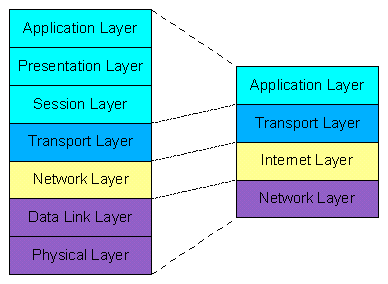
\includegraphics[scale=0.7]{../docs/tarkes/pics/ositcpip.png}
\end{center}
\subsection*{Client-Server Verhältnis$^{[207]}$}\label{ssec:client-server}
\addcontentsline{toc}{subsection}{Client-Server Verhältnis}
Das Client-Server Modell ist das bekannteste und am öftesten verwendete Muster für Aufgabenverteilung in einem Netzwerk.\\ 
Bei diesem Modell gibt es denjenigen, der die \textbf{Dienste anbietet, den Server}, und jenen, der die \textbf{Dienste nutzt, den Client}.\\

Mit dem Begriff \glqq Server\grqq können sowohl die Hardware als auch die Software gemeint sein.\\

\textbf{Hardware-Server} unterscheiden sich meistens nicht sehr von normalen Desktop-PCs, bis auf ihre Leistung, welche meistens auf ihre Aufgabe abgestimmt ist. Oft wird weniger Rechenleistung benötigt als RAM, ein anderes Mal umgekehrt. Manchmal wird auch viel Speicherplatz gebraucht.\\
Auch die Abmessungen variieren deutlich. Bei kleinen Servern, wie sie manche auch zuhause stehen haben, ist es oft nur ein normaler Tower, nur ohne Bildschirm, während große Firmen oder Organisationen häufig sogenannte \glqq Racks\grqq \ vollgestopft mit Blade-Servern stehen haben.\\
Ein Rack ist ein Gestell, in welches man Blade-Server einfach hineinschieben kann. Blade-Server (Blade, deutsch: Klinge) haben ihren Namen von ihrem überaus schlanken Design.\\

\begin{center}
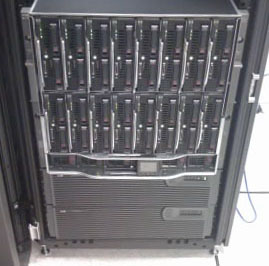
\includegraphics[scale=0.8]{../docs/tarkes/pics/ServerRack.jpg}\\
Ein Rack mit mehreren Blade-Servern 
\end{center}

Als \textbf{Software-Server} werden Programme bezeichnet, welche Dienste anbieten. Zu solchen zählt zum Beispiel der Webserver Apache, der FTP-Server Filezilla oder auch bind, die Referenzimplementierung eines DNS-Servers.\\
Software-Server werden häufig als \textbf{Dienste} oder \textbf{Deamons} bezeichnet. Sie laufen im Hintergrund, haben häufig, vorallem auf unixoiden Betriebssystemen, keine grafische Oberfläche, sondern lediglich mehr oder weniger viele Konfigurationsdateien und müssen so programmiert sein, dass sie großen Mengen an Anfragen begegnen können, ohne dass sie der Maschine, auf welcher sie laufen, ihre gesamten Resourcen wegfressen.\\

Clients sind ebenso vielfältig. Zu den Clients zählt jeder, der einen Dienst eines Servers in Anspruch nimmt. 
\subsection{Beispiel für Kommunikationsablauf}
Im Folgenden soll das Abrufen einer Seite von einem Web-Server, welcher in einem anderen Netzwerk steht, aus netzwerktechnischer Sicht, Schritt für Schritt besprochen werden.\\
\begin{enumerate}
\item Schritt:\\
Der User öffnet den Browser seiner Wahl und tippt die URL (Unified Resource Locater) in die Adressenleiste. Der Computer kann mit diesem Namen an sich nichts anfangen, also versucht er zuallererst in der Datei \glqq hosts\grqq , welche unter Windows im Dateipfad
\begin{lstlisting} 
C:\Windows\System32\drivers\etc\ 
\end{lstlisting} zu finden ist, und unter Unixoiden Betriebssystemen meistens unter 
\begin{lstlisting} 
/etc/
\end{lstlisting} liegt, nach einer zugewiesenen IP-Adresse für diesen Namen zu suchen.\\
Findet er eine IP-Adresse, fährt er mit Schritt 2 fort, ansonsten prüft der Rechner als nächstes seinen DNS-Cache nach einem entsprechenden Eintrag. Wurde die Seite bereits vor nicht allzu langer Zeit aufgerufen, besteht eine gute Chance, dass der entsprechende DNS Eintrag noch im Cache zu finden ist.\\
Auch hier fährt er bei Erfolg mit Schritt 2 fort. Sollte jedoch weder im Cache noch in der hosts Datei ein Eintrag zu dieser Seite stehen, muss der Rechner eine DNS-Anfrage durchführen.\\
\begin{enumerate}
\item Um eine DNS-Anfrage zu machen benötigt der Rechner zuerst die IP-Adresse des DNS-Servers. Die hat er entweder statisch eingetragen oder zusammen mit seiner IP-Adresse, dem Standart Gateway und anderen Konfigurierungsparametern beim DHCP bekommen.
\item Die IP-Adresse, welche er nun hat, vergleicht er mit seinem Netz, indem er die Subnetzadresse mit der IP-Adresse des Zieles und seiner eigenen bitweise UND verknüpft. Nun gibt es zwei Möglichkeiten: 
\begin{itemize}
\item Der DNS-Server befindet sich in seinem Netz
\item Der DNS-Server befindet sich nicht in seinem Netz
\end{itemize}
\item Für den Fall, dass sie sich im gleichen Netz befinden:\\
Der PC braucht nun die MAC-Adresse zu der IP-Adresse. Zuerst sieht er wieder nach, ob er sie gecached hat. Sollte er sie nicht im Cache liegen haben, schickt er einen ARP-Request. Dieses Protokoll frägt, wer denn eine bestimmte IP-Adresse hat, und ob derjenige ihm seine MAC-Adresse verraten würde. 
\item Für den Fall, dass sie sich nicht im gleichen Netz befinden:\\
Wenn der PC erkennt, dass sich das Ziel außerhalb seines Netzes befindet, schickt er es an den Default Gateway.\\
Der Default Gateway ist jene IP-Adresse, an die alles von allen geschickt wird, was sich nicht in ihrem Netz befindet, also muss auch jedes Netz einen Default Gateway haben. Die Gateway-Adresse gehört meistens zu einem Router, welcher dann anhand der IP-Adresse das Paket weiterleitet, bis es schlussendlich sein Ziel erreicht.\\
\item Nun verfügt der PC über alle Parameter die er braucht, um das DNS-Paket zusammenzubauen. TCP/IP Layer 1 hat die MAC-Adresse, TCP/IP Layer 2 die IP-Adresse, der Rechner weiß, dass DNS normalerweise auf UDP aufsetzt und kann deshalb Layer 3 den UDP Port 53 bestimmen und das DNS Paket selbst auf der Anwendungsschicht, dem TCP/IP Layer 4. Er öffnet noch einen Port über den 49151 als Source-Port, trägt diesen in das Paket auf dem Layer 3 ein, schickt das Paket ab und muss nur noch auf die Antwort, mit der IP-Adresse der Seite warten.
\end{enumerate}
\item Schritt:\\
Nun, da er über die IP-Adresse des Webservers verfügt, durchläuft der Rechner noch einmal alle Schritte, welche er bei der DNS-Anfrage durchlaufen hat, nur dieses Mal mit der IP-Adresse des Web-Servers, anstatt der des DNS-Servers.
\item Schritt:\\
Wenn er sich sämtliche Informationen, welche für diese Anfrage benötigt werden, gesammelt hat, baut er das HTTP-Request Paket zusammen, mit MAC- und IP-Adresse, diesesmal TCP Port 80, und der Seite im HTTP Teil des Paketes. Er wartet auf die Antwort Pakete, baut die Seite im Browser auf und der User bekommt, was er will.
\end{enumerate}
\section*{Protokolle$^{[208]}$}
\addcontentsline{toc}{section}{Protokolle}
Es gibt unzählige verschiedene Protokolle, hier soll nur auf ein paar wenige Wichtige eingegangen werden, welche auch Verwendung im praktischen Teil der Diplomarbeit gefunden haben.
\subsection{Ethernet}\label{ssec:eth}
\textbf{Ethernet} ist ein sowohl ein Layer1 als auch ein Layer2 Protokoll im OSI-Modell und damit für die unterste Schicht und den grundlegenden Kommunikationsmöglichkeiten zuständig.\\

Ethernet wurde ursprünglich für Lokale Netzwerke erdacht, weshalb es häufig als LAN-Technologie bezeichnet wird. Da das Protokoll vor über 30 Jahren begann zu existieren, wäre es natürlich nicht mehr ausreichend für heutige Anwendungen, doch es ist mit der Entwicklung des Internets mitgewachsen.\\
Während es anfangs nur für einzelne Häuser gedacht war, können inzwischen mittels Lichtwellenleitern Entfernungen von über 10 Kilometern überbrückt werden.\\

Auch die Datenrate wuchs zusammen mit dem Rest. Anfangs lief es nur über Twisted Pair oder Koaxial Kabel, während inzwischen der Lichtwellenleiter bis zum Endbenutzer in den Haushalt gefunden hat.\\

Da Ethernet über die Zeit so gewachsen ist, gibt es auch sehr viele verschiedene Standards. Hier soll nur auf ein paar der Neuesten eingegangen werden, da dies den Rahmen ansonsten sprengen würde.\\
\begin{itemize}
\item 10Gbit/s:
\begin{itemize}
\item Lichtwellenleiter Multimode:\\
10GBASE-SR\\
Zur Überbrückung kurzer Strecken mit langwelligem Licht, Reichweite je nach Leitungstyp zwischen 26 und 300 Metern.
\item Lichtwellenleiter Singlemode:\\
10GBASE-LW4\\
Zur Überbrückung langer Strecken mit Distanzen bis zu 10 Kilometern.
\end{itemize}
\item 40Gbit/s:
\begin{itemize}
\item 40GBASE-CR4\\
4 x Kupfer Twinax Kabel für Reichweiten von mindestens 4 Metern.
\item 40GBASE-LR4\\
Vier Farben Multimoden Lichtwellenleiter für Reichweiten von mindestens 10 Kilometern.
\end{itemize}
\item 100Gbit/s:
\begin{itemize}
\item 100GBASE-CR10\\
10 x Kupfer Twinax Kabel für Reichweiten von mindestens 7 Metern.
\item 100GBASE-ER4\\
4 Farben Singlemoden Lichtwellenleiter für Reichweiten von über 40 Kilometern.
\end{itemize}
\end{itemize}
Seit 2013 wird jedoch von einer Arbeitsgruppe der IEEE an einem Standard für 1TBit/s gearbeitet, der circa 2017 fertiggestellt werden soll.\\

Da die Wurzeln dieses Protokolls in einem gemeinsam genutzten Koaxial Kupfer Kabel liegen, war eines der Probleme sogenannte Kollisionen, also wenn zwei Rechner zur gleichen Zeit sprechen wollten.\\
Diesem Problem wurde mit dem \textbf{CSMA/CD} Algorithmus zu Leibe gerückt. CSMA/CD, was für Carrier Sense Multiple Access/Collision Detection steht, ist eine Weiterentwicklung des in den 1960 Jahren auf Hawaii verwendeten \textbf{ALOHAnet} Protokolls.\\
Dabei warten Teilnehmer des Netzwerkes immer, bis die Leitung nicht mehr belegt ist, bevor sie anfangen Daten zu übermitteln. Sollten jedoch zwei Rechner gleichzeitig beginnen zu reden, stoppen beide und warten eine zufällige Zeitdauer ab bis sie es erneut versuchen.\\
Obwohl nun seit einigen Jahren sowohl Full-Duplex Modus und Switches verwendet werden, welche Kollisionen verhindern, indem sie End-to-End Verbindungen erzeugen, befindet sich der Algorithmus bis zu den 10Gbit/s Standards immer noch zu den verwendeten Algorithmen.\\
Bei den höheren Netzen, wo CSMA/CD nicht mehr verwendet wird, wird ein extra Flowcontrol System verwendet. Bei CSMA/CD war das nicht notwendig, da eine Kollision sowieso eine Pause im Datenfluss hervorgerufen hat. Nun, ohne diesen Algorithmus, muss es jedoch trotzdem eine Möglichkeit geben, anderen zu vermitteln, dass eine Sendepause vonnöten ist. Dies wird bei Ethernet über 10Gbit/s mit einem bestimmten PAUSE Paket geregelt, in welchem die gewünschte Wartezeit notiert ist.\\

Ebenfalls in den Wurzeln des Protokolls verankert ist das \textbf{Broadcast Problem}.\\
Das Ethernet Protokoll hat sich nie um zielgerichtete Kommunikation gekümmert, weshalb es ohne weiteres alles an alle schickt. Das kann zu einem Problem werden, wenn ein Mensch mit böswilligen Absichten mitschreiben will, was im Netzwerk so passiert, denn das kann er dann tun.\\
Als noch Hubs verwendet wurden, war das Problem viel drastischer, denn ein Hub repliziert die Pakete, die er empfängt und schickt diese an alle Interfaces raus.\\
Switches hingegen schicken, wie bereits besprochen, Pakete nur an jenen Interfaces raus, wo auch das Ziel ist. Sie verhindern damit das sogenannte \glqq sniffen\grqq \ im Netzwerk.\\
Eine andere Option ist Verschlüsselung, auf welchen im Kapitel \ref{chap:krypto} auf Seite \pageref{chap:krypto} noch näher eingegangen wird. Diese verhindern jedoch nicht das sniffen ansich sondern sorgen dafür, dass der Cracker die Daten welche er mitliest nicht versehen kann.\\

\begin{center}
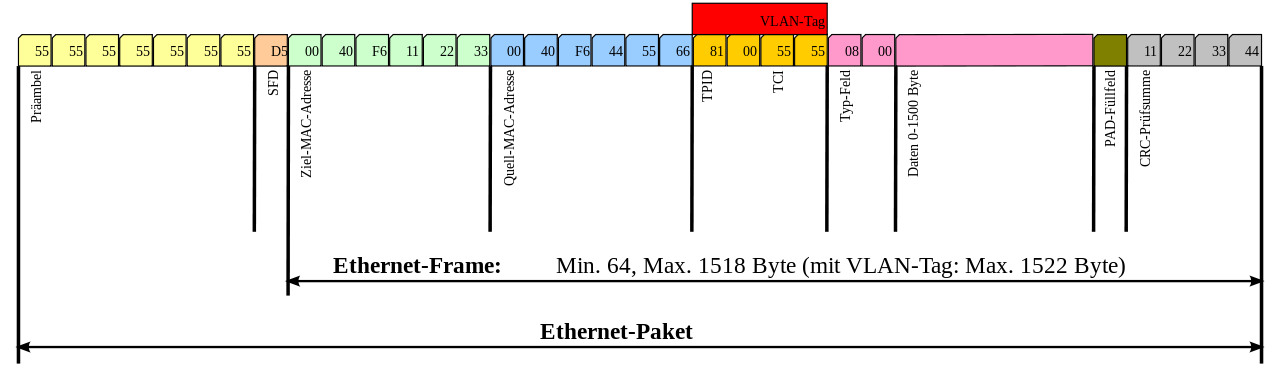
\includegraphics[scale=0.35]{../docs/tarkes/pics/Ethernetpaket.png}
Ethernetframe
\end{center}

Das Frame wird serialisiert und mit dem niederwertigsten Bit zuerst übertragen. Das EthernetframeF besteht aus folgenden Teilen:
\begin{itemize}
\item Präambel und SFD\\
Dieser Teil des Paketes sind im Grunde nur Überbleibsel aus den alten Tagen. Die Präambel hat ein alternierendes Bitmuster über 7 Byte, während der SFD (Start Frame Delimeter) das Muster 10101011 trägt.\\
Diese Felder wurden früher benötigt, um den einzelnen Devices eine Möglichkeit zu geben, sich auf die Bitabstände zu synchronisieren.\\
Die große Länge der Präambel liegt darin begründet, dass beim Passieren eines Repeaters oder Hubs immer ein Teil verloren ging. Um zu gewährleisten, dass auch bei maximal großen Netzwerken die Devices noch ein Minimum an Zeit haben sich zu synchronisieren, wurde die Länge auf 7 Bytes festgesetzt. 
\item Source- und Destination MAC-Adresse\\
Stehen für Quelle des Paketes und Empfänger des Paketes (siehe Kapitel \ref{sssec:macaddr} auf Seite \pageref{sssec:macaddr})
\item VLAN-Tag\\
Der VLAN-Tag ermöglicht das Auseinanderhalten von verschiedenen VLANs (siehe Kapitel \ref{sssec:vlan} auf Seite \pageref{sssec:vlan})
\item Typ Feld\\
Das Typ Feld oder EtherType Feld legt fest, welches Protokoll sich in der Payload befindet. So steht zum Beispiel der Wert 0x0800 für IP oder 0x0806 für ARP.
\item Payload\\
Die Payload oder Nutzlast ist die Nachricht, die das Ethernetframe mit sich nimmt. Diese kann nicht größer als 1500 bytes sein.
\item Pad bytes\\
Die Pad oder Padding bytes sind dazu da, das Ethernet Paket auf eine minimale Größe von 64 bytes zu bringen, da es bei den früheren Varianten ansonsten zu Problemen mit der Collisiondetection gegeben hätte.
\item FCS Feld\\
Das FCS (Frame Check Sequence) Feld beinhaltet eine 32 bit CRC Prüfsumme welche aus den Werten des reinen Layer2 Frames besteht. Also den bits von der MAC-Adresse bis hierher.
\end{itemize}

\subsection{Address Resolution Protocol - ARP}\label{ssec:arp}
\textbf{ARP} ist ein essentielles Protokoll für die Kommunikation in einem Netzwerk. Da, damit Kommunikation stattfinden kann, die MAC-Adresse bekannt sein muss, wurde dieses Protokoll entwickelt.\\
Es funktioniert folgendermaßen: Indem ein Broadcast in das Netz geschickt wird, in welchem die Bitte steht, dass ein Host mit einer gewissen IP doch seine MAC-Adresse übermitteln soll, kann ein Rechner die benötigte Information bekommen. Diese speichert der PC, der die Anfrage gestellt hat, in seinem lokalen Cache, damit er nicht jedes Mal nachfragen muss.\\
Dieses Protokoll wird mit der Verbreitung von IPv6 aussterben, da in IPv6 das sogenannte \textbf{Neighbour Discovery Protocol NDP} diese Aufgabe übernimmt.\\

Das ARP Paket befindet sich gleichzeitig auf Layer2 und 3 und sieht wie folgt aus:\\
\begin{itemize}
\item Hardwareadresstyp\\
Die Zahl in diesem Feld bestimmt den Typen der MAC-Adresse. Dies ist meistens Ethernet, was mit einer 1 repräsentiert wird.
\item Protokolladresstyp\\
Der Adresstyp für den die MAC-Adresse angefordert wird. Im Falle von IP ist dies 0x0800. Die Zahlen in diesem Feld teilen sich ihre Nummern mit dem EtherType beim Ethernet Protokoll.
\item Hardwareadresslänge\\
Die Länge der aufgelösten Adresse. Für Ethernet ist sie 6.
\item Protokolladresslänge\\
Die Länge der Adresse, die aufgelöst werden soll. Für IPv4 lautet sie 4.
\item Operation\\
Enthält eine Zahl, die angibt, ob das Paket ein Request (1) oder eine Response (2) ist.
\item Quell MAC-Adresse
\item Quell IP-Adresse
\item Ziel MAC-Adresse\\
Enthält FF:FF:FF:FF:FF:FF, die Layer2 Broadcast Adresse.
\item Ziel IP-Adresse
\end{itemize}
Es gibt jedoch auch noch andere Arten von ARP Paketen. Dazu zählen der Reverse ARP, welcher die MAC- in eine IP-Adresse auflösen kann oder der Gratuitos ARP, welcher eine Nachricht darstellt, die unaufgefordert bekannt macht, welche MAC-Adresse man selbst hat.
\subsection{Internet Protocol - IP}\label{ssec:ip}
Das \textbf{Internet Protokoll} hat zwei Hauptaufgaben:
\begin{itemize}
\item \textbf{Adressierung}\\
Das Ziel der Adressierung auf dieser Ebene ist es, wie bereits zuvor besprochen, ein Gerät über mehrere Netzwerke hinweg eindeutig zu machen, um Pakete nicht nur innerhalb eines Netzwerkes sondern über mehrere Netzwerke hinweg ansprechen zu können.
\item \textbf{Fragmentierung}\\
Da Kommunikation sich ja meistens nicht mit nur einem Paket ausgeht, ist es wichtig, dass Kommunikationsstränge aufgeteilt werden können in mehrere kleine Pakete. Dies nennt man dann Fragmentierung. IP ist dafür zuständig, dass fragmentierte Pakete wieder zusammenfinden können, da es ja nicht heißen muss, dass nur eine einzige Kommunikation gerade am Laufen ist.\\
Dies gilt jedoch nur mehr für IPv4, denn in IPv6 ist es nicht mehr vorgesehen, dass Pakete fragmentieren.
\end{itemize}
\subsubsection{IPv4}
IP Version 4 war der erste offizielle Standard des Internet Protocols.\\
Adressierung im Schema von IPv4 wurde bereits in Kapitel \ref{sssec:ipaddr} auf Seite \pageref{sssec:ipaddr} besprochen.\\

Es gibt einige gesonderte Adressbereiche in IPv4, welche nicht für die öffentliche Nutzung verwendbar sind. Dazu zählt:
\begin{itemize}
\item 10.0.0.0/8\\
Sogenanntes Class A Netz: 1 Netz mit 16.777.216 Adressen (erstreckt sich bis 10.255.255.255/8)
\item 172.16.0.0/12\\
Sogenanntes Class B Netz: 16 Netze mit jeweils 65.536 Adressen (erstreckt sich von 172.16.0.0/16 über 172.17.0.0/16 usw. bis 172.32.0.0/16)
\item 192.168.0.0/16\\
Sogenanntes Class C Netz: 256 Netze mit je 256 Adressen (erstreckt sich von 192.168.0.0/24 über 192.168.1.0/24 usw. bis 192.168.255.0/24)
\item 100.64.0.0/10\\
Der sogenannte Shared Adress Range. Er ist speziell für Internet Service Provider und ihre Anforderungen beim NAT bestimmt und nicht für den normalen User gedacht.
\item 169.254.0.0/16\\
Link Local Adressbereich. Er wird verwendet, wenn keine spezifische IP-Adresse einem Rechner zugewiesen wird. Damit sind auch zwei Clients in der Lage miteinander zu reden, wenn sie unkonfiguriert und ohne DHCP-Server entweder direkt durch Kabel oder über einen Switch verbunden sind.
\item 127.0.0.0/8\\
LoopBack. Dieser Adressbereich wird für Interfaces des Hosts selbst verwendet. 
\item ...\\
Es gibt noch einige Bereiche mehr, aber es würde hier zu weit führen alle aufzuzählen. Sie können in der RFC6890 (zum Zeitpunkt des Schreibens aktuelle Version) nachgelesen werden.
\end{itemize}

Obwohl IPv4 schon seit mehreren Jahren von IPv6 abgelöst wurde, sind bis heute die wenigsten Firmen und noch weniger Heimnetzwerke auf IPv6 umgestellt. Es wird also im Grunde noch überall IPv4 verwendet, obwohl der Adressbereich ($2^{32} = 4.294.967.296$, abzüglich reservierter Adressen = 3.707.764.736) in dieser Version bereits \textbf{vollständig aufgebraucht} ist.\\

Dieser Problematik wurde mit einigen Zwischenlösungen begegnet. Das Protokoll \textbf{NAT (Network Address Translation)} ist eines dieser Behilfsmittel.\\
Der IPv4 Standard sieht eine Aufteilung in öffentliche und private Netzwerke vor. Adressen, welche aus dem Bereich der Privaten Netzwerke kommen, müssen nicht eindeutig sein und können so oft wie gewünscht verwendet werden. Durch ihre Mehrdeutigkeit sind sie jedoch auch nicht dazu geeignet, im Internet verwendet zu werden, sondern sie sind für den privaten Gebrauch gedacht, daher auch Privates Netzwerk.\\
Will man nun aus seinem privaten Netz raus in das Internet, wendet jener Router, welcher das private Netz mit dem des Providers verbindet, NAT an.\\
Er legt dabei eine Tabelle an, in welcher die private Adresse sowie der Port steht, und ersetzt diese durch eine öffentliche Adresse und einen beliebigen anderen High Port. Die Antworten weist er anhand des Ports dann wieder der richtigen privaten Adresse zu und leitet diese vom Internet zu dem Host, der die Anfrage abschickte.\\
Dadurch scheint es, als würden mehrere Hosts die gleiche IP-Adresse haben, nämlich jeder, welcher über diesen Router das private Netzwerk verlässt.\\

Eine andere Art, mit der das unausweichliche Versiegen an Adressen versucht wurde hinauszuzögern, ist die \textbf{dynamische Adressenvergabe von Providern an ihre Kunden}.\\
Sieht man sich mithilfe von externen Tools die Adresse, welche man nach außen hat, an zwei verschiedenen Tagen an, kann es sein, dass sich diese unterscheiden.\\
Der Provider verwendet diese Methode, um mehrere Kunden mit Adressen zu versorgen, als er eigentlich hat. Er geht dabei davon aus, dass zu keiner Zeit alle seine Kunden gleichzeitig online sind.\\

Das Problem entwickelte sich daraus, dass anfangs die Meinung geläufig war, es seien weitaus genug Adressen verfügbar. Deshalb hat man große Adressbereiche billig an Universitäten und Organisationen oder Firmen verkauft, ohne einen Gedanken daran zu verschwenden, dass womöglich irgendwann keine Adressen mehr übrig sein könnten.\\
Offiziell wurden im \textbf{Januar 2011} die letzten beiden verfügbaren IPv4 Netze der RIR (Regional Internet Registry) von der IANA (Internet Assigned Numbers Authority) zugewiesen, welche diese nun an die einzelnen Länder aufteilen.\\

Warum die Verwendung des IPv6 Standards trotzdem soweit hinausgezögert wird, liegt an der Starre der Firmen. Die Umstellung auf IPv6 bedeutet viele Probleme, da, obwohl er bereits von fast jeglicher Hardware unterstützt, immer noch Kompatibilitätsprobleme mit sich bringt. Firmen sehen keinen Sinn darin viel Geld zu investieren, um etwas zu implementieren, was doch sowieso funktioniert.\\

Der IP-Header sieht wie folgt aus:\\
\begin{center}
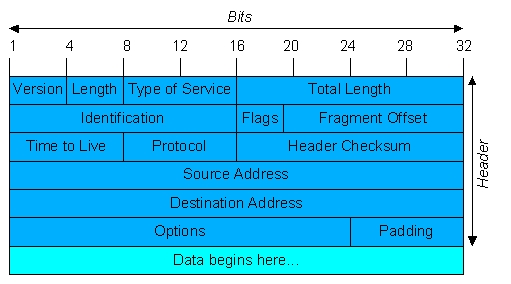
\includegraphics[scale=1]{../docs/tarkes/pics/ipheader.jpg}
\end{center}
\subsubsection{IPv6}
IPv6 ist der offizielle Nachfolger von IPv4. Er ist seit 1998 von der IETF standardisiert und bringt einige Neuerungen in das Internet Protocol welche die Fehler, die durch das unterschätzte Wachstum des Internets hervorgerufen wurden, aufheben soll.\\

Eine dieser Neuerungen, wahrscheinlich auch die wichtigste, ist der \textbf{vergrößerte Adressbereich}. Während IPv4 $2^{32}$, also etwas mehr als 4 Milliarden Adressen hat, verfügt IPv6 über $2^{128}$, umgerechnet über 340 Sextillionen oder $3,4 \cdot 10^{38}$ Adressen.\\
Ein anschaulicheres Beispiel bietet folgender Vergleich: Das Alter der Erde wird auf etwa 4,5 Milliarden Jahre geschätzt. Hätte man gleichzeitig mit der Entstehung der Erde begonnen mit einer Rate von 1 Milliarde Adressen pro Sekunde IPv6 Adressen aus dem vorhandenen Adressraum zu verteilen, wäre bis heute nur weniger als ein Billionstel des vorhandenen Adressraums vergeben.\\
Damit dürfte das Problem des Adressenmangels vorübergehend gelöst sein.\\

Weitere Vorteile sind das Anpassen der Headers an die neuen Anforderungen.\\
So ist beispielsweise IPsec bereits im IPv6 selbst implementiert. Auch der Rechenaufwand für Router soll damit minimiert werden.\\

Eine Aufgabe, die IPv6 nicht länger vollbringt, wird das zuvor erwähnte Fragmentieren sein. Wenn ein Router ein Paket bekommt, welches größer ist als sein MTU (Maximal Transition Unit), verwirft er das Paket und sendet ein ICMPv6 Paket mit der Meldung \glqq Too Big\grqq . Es ist nun die Aufgabe der Schichten darüber dafür zu sorgen, dass die Pakete, welche sie versenden wollen, nicht zu groß sind.\\

Die Adressnotation in IPv6 ist deutlich anders als bei IPv4. Es gibt aufgrund der Länge und schweren Handhabbarkeit der Adressen einige Vereinfachungsregeln, welche darauf abzielen, die Adressen zu kürzen. Da die Adressen sehr viel länger sind, kommt eine dezimale Notation, wie sie vorher Verwendung fand, nicht mehr in Frage.\\
IPv6 verwendet daher Hexadezimale Notation, teilt die Adresse in 8 Blöcke auf und fasst in jedem Block 16 bit (=4 Hexadezimalstellen) zusammen. Die Blöcke werden durch Doppelpunkte getrennt: \textbf{2001:0db8:85a3:08d3:2219:8a2e:0370:7344}\\
Führende Nullen dürfen dabei ausgelassen werden.\\ \textbf{2001:0db8:85a3:08d3:0000:8a2e:0070:7344} entspricht also\\ \textbf{2001:db8:85a3:8d3:0:8a2e:70:7344}\\
Kontinuierliche Blöcke aus 0 dürfen komplett ausgelassen und durch einen zweifachen Doppelpunkt angezeigt werden. Diese Maßnahme darf jedoch nur einmal Verwendung finden, da es sonst zu Mehrdeutigkeiten kommen kann. Beispiel: \textbf{2001:0db8:85a3:0:0:8a2e:0:0} darf entweder als \textbf{2001:0db8:85a3::8a2e:0:0} oder als \textbf{2001:0db8:85a3:0:0:8a2e::} geschrieben werden.\\

Die \textbf{128 bit} lange Adresse wird in \textbf{zwei 64 bit} große Teile aufgeteilt. Ersterer ist der sogenannte \textbf{Präfix}.\\
Die letzten 64 bit jedoch sind der für jede Netzwerkschnittstelle eindeutige \textbf{Network-Identifier}. Dieser wird anhand der MAC-Adresse ausgerechnet.\\
Daraufhin wurde Kritik aus der Internetgemeinde laut, da so die Anonymität des Internets vollständig verloren gehen würde. Die IETF hat daraufhin mit der RFC4941 die \textbf{Privacy Extensions} eingeführt, welche den Host selbstständig zufällig generierte Network Identifiers machen lässt. Dieser ist in den meisten Betriebssystemen standardmäßig aktiv.\\
Dies erhöht die Anonymität zwar, reicht aber noch nicht, solang der Präfix, welcher meistens vom ISP vorgegeben wird, ebenso eindeutig ist. Sollte dieser ebenso dynamisch vergeben werden, ist ein guter Teil der Anonymität, welche IPv4 hatte, wieder gegeben.\\

Wenn eine IPv6 Adresse als URL verwendet werden soll, wird sie in eckige Klammern geschrieben, damit einer Verwechslung mit der Portnummer als Teil der Adresse vorgebeugt wird.\\

Da es keine privaten Netze mehr gibt, fallen viele reservierte Adressbereiche weg. Ein paar Wesentliche sollen trotzdem genannt werden:
\begin{itemize}
\item ::1/128\\
Die LoopBack Adresse, entspricht 127.0.0.1 bei IPv4
\item fe80::/10\\
Link Local, entspricht 169.254.0.0 bei IPv4, wird verwendet für die Neighbour-Discovery und Autoadresszuweisungen.
\item 2000::/3 - 3fff::/3\\
Momentaner Bereich für global eindeutige Adressen.
\item 2001::\\
Werden den ISPs für ihre Kunden gegeben.
\item 2001:0db8::/32\\
Für Dokumentationszwecke
\item ...\\
Auch hier kann wieder in der RFC 6890 nachgelesen werden, um mehr zu erfahren.
\end{itemize}
\subsection{User Datagram Protocol - UDP}
Mit der Entwicklung von UDP wurde 1977 begonnen, als ersichtlich wurde, dass es notwendig ist, ein Übertragungsprotokoll zu spezifizieren, welches \textbf{schneller war als TCP}. UDP setzt auf IP auf und implementiert, gleich wie TCP, Ports.\\

Durch den Fokus auf die Geschwindigkeit der Datenübertragung wurden dafür an einigen anderen Punkten Abstriche gemacht. So ist es im Gegensatz zu TCP \textbf{nicht verbindungsorientiert}, was bedeutet, dass es von sich aus nicht dafür Sorge trägt, ob Pakete, welche über das Netzwerk geschickt werden, auch am anderen Ende ankommen, noch ob sie in dort richtigen Reihenfolge ankommen.\\
Auch \textbf{sicherheitstechnisch ist keine Absicherung vorhanden}. UDP an sich hat keine Vorkehrungen dafür getroffen, dass der Inhalt der Pakete geheim bleibt bzw. dass er unverändert ankommt.\\

UDP hat trotz dieser Mängel große Bedeutung. Anwendungen, bei denen das Fehlen von einzelnen Paketen nicht allzu schlimm ist, wie zB. VoIP (Voice over IP) oder bei denen nur kurze Paketwechsel stattfinden, ein Verbindungsaufbau also nur übermäßig Traffic erzeugen würde, wie zB DNS.\\

Der UDP Header beinhaltet folgende Werte: 
\begin{itemize}
\item Source Port
\item Destination Port
\item Länge
\item Checksum\\
In diesem Feld wird eine Prüfsumme vom Header und dem Paket erzeugt. In IPv4 ist dies noch optional, bei IPv6 nicht mehr.
\end{itemize}
\subsection{Transmission Control Protocol - TCP}
Die Entwicklung von TCP dauerte einige Jahre. Es begann bereits 1973, endete aber erst 1981 mit der Veröffentlichung der RFC 793. TCP ist ein \textbf{zuverlässiges, verbindungsorientiertes Protokoll}. Es stellt damit sowohl Flusssteuerung und Staukontrolle als auch das Vorhandensein aller Daten in der richtigen Reihenfolge sicher.\\

\begin{center}
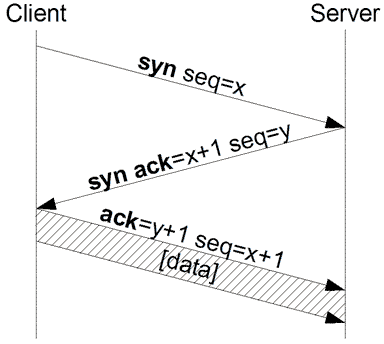
\includegraphics[scale=0.6]{../docs/tarkes/pics/TcpHandshake.png}
\end{center}

Da TCP ein verbindungsorientiertes Protokoll ist, gibt es auch einen Verbindungsaufbau.\\
Dieser findet mittels eines \textbf{Three-Way-Handshake} statt: Zuerst wird vom Client ein \textbf{SYN Paket} (ein Paket, bei welchem das SYN-Flag im Header gesetzt ist) an den Server geschickt. Der Wert im Sequence-Feld ist dabei zufällig gewählt.\\
Der Server schickt dann ein \textbf{SYN-ACK Paket} zurück, indem, zusätzlich zu der SYN-Flag auch noch das ACK-Flag gesetzt ist. Im Acknowledge-Feld steht dabei der Wert des Sequence-Feldes des SYN-Paketes des Clients, während im Sequence Feld des SYN-ACK Paketes eine neue zufällige Zahl steht.\\
Das dritte Paket des Verbindnungsaufbaus ist dann das \textbf{ACK-Paket} des Clients an den Server. Darin ist nur noch das ACK-Flag gesetzt, im Sequence Feld steht der Wert des ersten Paketes + 1 und im Acknowledge Feld steht der Wert aus dem Sequence Feld des vorherigen Paketes.\\

Daraufhin ist der Verbindungsaufbau abgeschlossen und die Datenübertragung kann beginnen.\\
Dabei wird die Ordnung und Sicherheit, dass jedes Paket auch wirklich ankommt, dadurch erreicht, dass der Empfänger jedes Paket, welches ihm in seiner Liste fehlt, noch einmal anfordert und das so oft, bis er es auch bekommt. Ob ihm eines fehlt, erkennt er anhand des Sequence Feldes.\\
Er buffert diese Pakete dann eine gewisse Zeit, um fehlende Elemente nachzuholen, doppelte zu verwerfen und sie in Reihenfolge zu bringen.\\

Der TCP Header:\\
\begin{itemize}
\item Source Port
\item Destination Port
\item Sequence Number\\
Wie bereits zuvor erwähnt, dient diese dazu, Ordnung halten zu können und um zu sehen, ob doppelte oder vermisste Pakete existieren.
\item Acknowledge Number\\
Für den Verbindungsaufbau
\item Data Offset\\
Größe des Headers, gibt den Beginn der Nutzdaten an
\item Reserved\\
Wird nicht verwendet und muss 0 sein
\item Control Flags\\
Es gibt einige verschiedene Control Flags. Zwei davon, SYN und ACK, wurden bereits erwähnt. Des Weiteren gibt es noch beispielsweise FIN für den Verbindungsabbau, URG für Urgent, also dringende Pakete oder RST für Reset.
\item Window \\
Die Menge an Daten, die der Client zu empfangen bereit ist.
\item Checksum
\item Urgent Pointer\\
Nur wichtig, falls das URG Flag gesetzt ist
\item Options\\
Hier kann noch alles Mögliche ausgemacht werden, welches nicht im Standardheader steht.
\end{itemize}
\subsection{Dynamic Host Configuration Protocol - DHCP}\label{ssec:dhcp}
DHCP dient, wie der Name bereits aussagt, der \textbf{dynamischen Konfiguration} von Hosts. Standardmäßig hat jeder normale Enduser in dem WLAN Router, welchen er von dem ISP bereitgestellt bekommt, einen DHCP-Server. Dieser nutzt jedoch nur die grundlegendsten Funktionen des DHCP Protokolls, die Vergabe einer \textbf{IP-Adresse und eines Standard Gateways}.\\
DHCP ist jedoch zu weit mehr in der Lage. Die Optionen reichen von Hostnamen über Proxy Einstellungen bis zu Zeitservern. Im Grunde sind die Optionen zur Konfiguration jedoch sogar unbegrenzt, da im Optionen Feld des Paketes eigene Dinge spezifiziert werden können.\\

Der Ablauf einer Kommunikation zwischen Host und DHCP-Server sieht wie folgt aus:\\
Ein Client, ahnungslos und ohne eigene Adresse, schreit in das Netzwerk, ob denn ein DHCP Server existiert, welcher ihm eine Konfiguration anbieten möchte. Dieses Paket ist das \textbf{DHCPDISCOVER}.\\
Niemand, einer oder mehrere Server, je nach Bestückung des Netzwerkes, antworten nun mit einem \textbf{DHCPOFFER}, in denen sie eine Konfiguration anbieten.\\
Der Client wählt nun eine der angebotenen Konfigurationen und teilt das dem Netzwerk mit einem \textbf{DHCPREQUEST} mit.\\
Der Server, welchem der Request gilt, kann dieser nun mit \textbf{DHCPACK} für Acknowledge zustimmen oder mit \textbf{DHCPNACK} für Not Acknowledge ablehnen.\\

DHCP Header:\\
\begin{center}
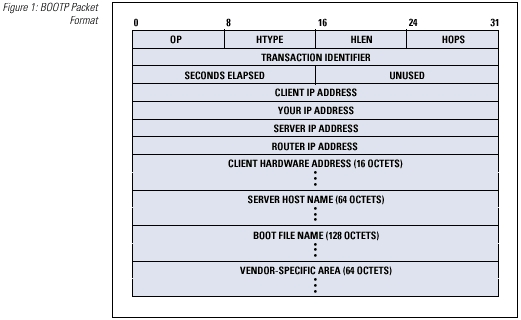
\includegraphics[scale=0.7]{../docs/tarkes/pics/dhcpheader.jpg}
\end{center}
\subsection{Domain Name System - DNS} \label{ssec:DNS}
DNS ist ein Protokoll, welches zwar nicht zwingend notwendig ist für das Funktionieren des Internets, aber uns Menschen es sehr komfortabel macht damit zu arbeiten.\\
Jeder ist heutzutage gewohnt, durch simples Eintippen eines Namens, zu einer Seite zu kommen. Dies wird jedoch erst durch DNS möglich. Ein PC selbst \textbf{kann mit dem Namen nichts anfangen, er muss ihn auflösen}. Dafür schickt er den Namen zu seinem eingetragenen DNS Server und bittet ihn um die zugehörige IP-Adresse.\\

Würde nun jedoch jeder DNS Server jeden Namen mit dazugehöriger IP-Adresse speichern, würde es sehr schnell außer Kontrolle geraten. Deshalb ist DNS \textbf{hierarchisch} designed. Das bedeutet, dass ein DNS-Server nur für einen gewissen Bereich zuständig ist. Weiß er nicht weiter, geht er die Leiter solange hinauf, bis er schließlich jemanden findet, der, wenn er auch vielleicht den Namen an sich nicht weiß, ihn zu dem führen kann, der ihn weiß.\\
Das kann im schlimmsten Fall bei einem der Root Name Server enden, der höchsten Autorität.\\

Zum besseren Verständnis sollte eine typische URL erklärt werden:\\
\textbf{www.example.com} besteht aus mehreren Bestandteilen.
\begin{itemize}
\item .\\
Nach dem kompletten Namen ist eigentlich ein Punkt, der jedoch inzwischen ausgelassen werden kann
\item com\\
Die Top Level Domain \glqq com\grqq . Zu den Top Level Domains gehören auch die Länder Domains wie zum Beispiel at, us, jp und so weiter. Eine Domain ist eine Zusammenfassung von mehreren verschiedenen Untergruppen. So indiziert die Länder Domain at, dass alle URLs, welche auf diese Top Level Domain enden, in Österreich ihren Standpunkt haben.
\item example\\
example wäre in diesem Beispiel eine Subdomain. Häufig werden Subdomains von Firmen und Organisationen gekauft. 
\item www\\
Obwohl das dreifache w im Internet immer mehr verloren geht, haben sie eigentlich eine wichtige Bedeutung. Sie sind der Eine unter allen Hosts welche sich in dieser Domain befinden, auf den man zugreift. Erst hier spitzt sich der Name auf einen Server zu. 
\end{itemize}
Nun wird auch ersichtlich, warum ein hierarchisches System sinnvoll ist.\\

Dies wird auch vom Staat genutzt, um Zensur zu betreiben. Die Filme und Serien Streaming Seite kinox.to wurde aus den DNS Servern in Deutschland gelöscht, als Konsequenz auf die Urheberrechtsverletzungen.\\

DNS Header:\\
\begin{center}
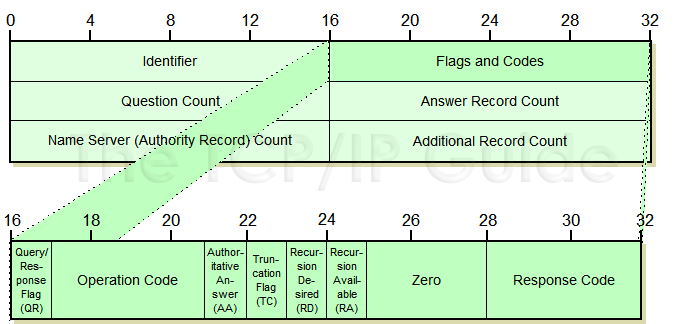
\includegraphics[scale=0.7]{../docs/tarkes/pics/dnsheader.png}
\end{center}
\subsection{Internet Control Message Protocol - ICMP}
Das Internet Control Message Protocol bewegt sich auf Layer 3 zusammen mit IP. Es dient dazu, anderen Geräten \textbf{Informationen über ihren Status} zukommen zu lassen. Es gibt eine Variante für IPv6, das sogenannte ICMPv6. Es verwendet zum Transport IP, obwohl es auf dem gleichen Layer liegt, da es sich als ein Protokoll höherer Ebene interpretiert.\\

Der Header des ICMP Paketes ist sehr klein. Er besteht lediglich aus:
\begin{itemize}
\item Type\\
Stellt die Art des ICMP dar. Kann zB. 3 für \glqq Ziel nicht erreichbar\grqq \ sein.
\item Code\\
Bietet eine genauere Auflösung der Art. Wenn der Typ zB. 3 ist, gibt es die Codes 0 für \glqq Netzwerk nicht erreichbar\grqq , 1 für \glqq Host nicht erreichbar\grqq , 2 für \glqq Protokoll nicht erreichbar\grqq \ und noch einige andere.
\item Checksum
\item Daten
\end{itemize}

Wichtige Beispiele für die Funktionen dieses Protokolls sind die Meldungen \textbf{Host Unreachable} oder \textbf{Destination Port Unreachable} für die Berichterstattung, es gibt aber auch Analysefunktionen wie traceroute oder den ICMP Echo Request. 
\paragraph{Echo Request/Response - Ping}
Der ICMP Echo hat die Typen Nummer 0. Er wurde durch das \textbf{Netzwerkprogramm Ping} auch unter diesem Namen bekannt.\\
Es wird verwendet um zu überprüfen, ob ein gewisser Host im Netzwerk ist oder nicht. Wenn ein Host ein Echo Paket empfängt, antwortet er mit einem Response Paket, genannt Pong.\\

Die Namensgebung kommt vom Sonar in U-Booten, die jedes Mal ein Ping von sich geben, wenn sie ihre Schallwellen aussenden, und ein Pong, wenn die Schallwellen von etwas reflektiert werden.\\ 
Gleich wie beim Sonar kann aus dem Echo Paket einiges an Information ausgelesen werden. So gut wie immer ist die Round-Trip Time, also die Zeit, die ein Paket benötigt, um vom Sender zum Ziel und wieder zurück zu kommen, dabei sowie der Wert aus dem Time To Live Feld, also wie viele Hops es noch passieren kann, bevor es verworfen wird.
\subsection{File Transport Protocol - FTP}
Das File Transport Protocol ist, wie der Name schon sagt, ein Protokoll zum \textbf{Übertragen von Dateien}. Es setzt auf TCP auf, da es sich nicht erlauben kann, dass Pakete verloren gehen, weil ansonsten die gesamten Daten unbrauchbar werden können. TCP verwendet \textbf{getrennte Verbindungen} für Data Transfer und Command Transfer. FTP antwortet auf Commands mit \textbf{dreistelligen Zahlen Codes} wie 200 für OK.\\

Um eine Verbindung aufzubauen, öffnet ein Client eine TCP Verbindung zum Port 21 von einem zufälligen Port N aus. Von diesem Zeitpunkt an wird es wichtig, ob der FTP Server als \glqq aktive\grqq \ oder als \glqq passive\grqq \ betrieben wird.\\
Bei einem als aktiv konfigurierten Server wartet der Client nun auf dem Port N+1 auf eine einkommende Datenverbindung. Damit der Server weiß, auf welchen Port er die Verbindung aufbauen soll, wird in der Command Verbindung ein PORT Befehl gesendet.\\
Sollte der Server als passiv konfiguriert sein, was häufig bei Servern hinter einer Firewall gemacht wird, sendet der Client ein PASV Paket über die Command Verbindung und bekommt daraufhin vom Server eine IP und einen Port, auf welchen daraufhin die Datenverbindung aufgebaut wird.\\

Ein großes Problem von FTP ist, dass, auch wenn es durch Username und Passwort geschützt werden kann, alles in Klartext überträgt. Es ist also für einen unerwünschten Mithörer im Netzwerk nicht sehr schwer alles mitzubekommen, was zwischen FTP Client und Server an Kommunikation passiert.\\
Um dies zu umgehen gibt es einige Varianten von FTP, welche Sicherheit garantieren sollen, wie u.a. \textbf{FTPS (File Transport Protocol SSL/TLS) oder SFTP (SSH File Transport Protocol)}, welche trotz des ähnlichen Namens unterschiedlich realisiert sind. 
 
\subsection{Simple Network Managing Protocol - SNMP}
Das SNMP dient dazu, die Pakete zu beschreiben, mit welchen Informationen zwischen verschiedenen Netzwerkgeräten ausgetauscht werden können. Diese Informationen finden sich in einer \textbf{MIB}. Es setzt auf UDP auf.\\

MIBs oder Management Information Bases sind \textbf{Tabellen mit beschreibenden Werten}. Diese Werte sind in einer \textbf{Baumstruktur} angeordnet. Der für SNMP interessante Bereich beginnt bei 1.3.6.1, dem Internet Zweig. Was in der MIB steht, ist von der IETF vorgegeben. SNMP weiß jedoch nicht, mit welchem Device es gerade redet, weshalb es nur als \glqq Bote\grqq für die Informationen dient.\\
Die Informationen, welche damit abgerufen werden können, sind unglaublich vielfältig und umschließen sogar Dinge wie Fehlerpakete auf einem bestimmten Interface auf einem Host.\\

Die MIB:
\begin{center}
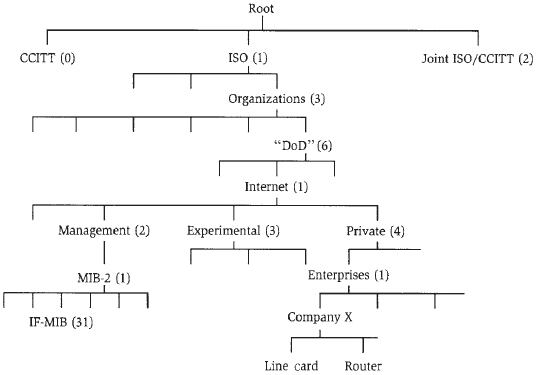
\includegraphics[scale=0.7]{../docs/tarkes/pics/mib.jpg}
\end{center}

Es gibt inzwischen \textbf{drei Versionen} von SNMP. Der Hauptkritikpunkt an den ersten Versionen war die Unsicherheit. Es ging so weit, dass im Scherz behauptet wurde, SNMP stehe eigentlich für \textbf{S}ecurity? \textbf{N}ot \textbf{m}y \textbf{P}roblem. Dies wurde auch erst mit der letzten Version, Version 3 wirklich ausgebessert.\\
Davor wurde nur mit einem sogenannten \textbf{Community String}, welches eine Art Passwort darstellt, gesichert und selbst dieser wurde in Klartext übermittelt.\\
Dies wurde in Version 3 dann verbessert und mit zwei zusätzlichen Passphrasen, genannt \textbf{Authentification und Privacy}, welche mit verschiedenen Verschlüsselungen versehen werden können, hinzugefügt wurden.\\

\begin{center}
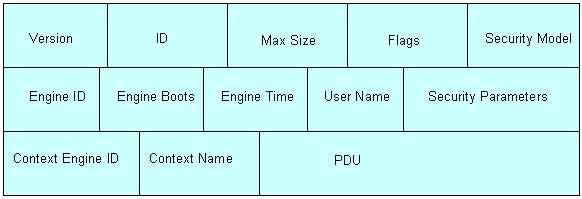
\includegraphics[scale=0.7]{../docs/tarkes/pics/snmpheader.jpg}
\end{center}

Es gibt mehrere Möglichkeiten wie SNMP Informationen aus einer MIB bekommt. Der Standard ist die \textbf{GET Methode}, bei der er ein Feld abfrägt. Doch gibt es auch die Methoden \textbf{GETNEXT und GETBULK}.\\
Bei ersterer Methode wandert er eine spezifizierte Anzahl an Werten ab. Diese Methode wurde erst in Version 2 dazugenommen.\\
Bei zweiterer Methode erfrägt er einen gesamten Unterbaum.\\

Des Weiteren gibt es noch eine Sonderform, in welcher nicht der Agent, so wird derjenige genannt, welcher die SNMP Abfragen durchführt, sondern das zu managende Device selbst sich meldet.\\
Diese sogenannten \textbf{Traps} können auf bestimmte Events gesetzt werden, wie zB. eine Änderung eines kritischen Wertes. Bei weitem öfters wird es jedoch verwendet, wenn eine der Zähler Variablen überläuft. Dabei setzen MIBs meist ein Flag in einem bestimmten Unterbaum, auf welches die Traps dann reagieren.\\

Obwohl das Protokoll sich selbst als \glqq Simple\grqq \ bezeichnet, ist es hoch komplex und, obwohl es von einem großen Teil ernstzunehmender Administratoren genutzt wird, bringt es auch extreme Sicherheitsprobleme mit, wenn man es nicht vorsichtig implementiert.\\
Vorallem die Tatsache, dass SNMPv3 Support, obwohl es ein Standard ist, so gut wie nirgends gegeben ist (unter anderem unterstützt Windows bis jetzt nur SNMPv2(c)), macht es große Probleme. 
\subsection{Hypertext Transfer Protocol - HTTP}
HTTP ist wohl eines der Protokolle, welches der Standarduser am häufigsten verwendet, auch wenn er sich dessen unter Umständen gar nicht bewusst ist. Es wird verwendet, um \textbf{Webseiten über ein Netzwerk zu transportieren}. HTTP befindet sich auf den Layern 5 bis 7 und setzt auf TCP auf, da sich vermisste oder fehlerhafte Pakete doch deutlich in der Seitendarstellung auswirken.\\
Momentan wird \textbf{HTTP/1.1} verwendet, wobei die HTTP-Entwicklergruppe der IETF bereits dabei ist, Version 2 zu spezifizieren. Ziele der neuen Version sind bessere Datenkomprimierung, effizientere Kommunikation und erhöhte Sicherheit.\\

Sicherheitstechnisch ist HTTP nicht sehr ausgefeilt. Es verwendet keine Verschlüsselung von sich aus, überträgt alles in Klartext. Dafür wurden diverse Erweiterungen geschrieben, wie zum Beispiel \textbf{HTTPS, welches Pakete mit SSL Verfahren sichert}.\\

Aufgrund diverser Erweiterungen in den Anfragenpaketen ist HTTP inzwischen über den bloßen Transport von Hypertext hinaus, es kann bereits genauso zur Übertragung von zB. Dateien verwendet werden.\\

Eine Kommunikation mit HTTP läuft immer nach einem gewissen Schema ab:\\
Ein Client schickt eine Anfrage an eine URL, wie zB. www.example.com ab. Dieser Name wird, wie bereits besprochen, über DNS aufgelöst, sollte er nicht in der hosts Datei stehen.\\
Der Webbrowser setzt an die URL normalerweise immer noch \glqq \textbackslash index.html \grqq .\\
Dies wandelt der Browser dann in ein HTTP GET Paket um, in dem neben der verwendeten HTTP Version steht, was man von welchem Client bekommen will.\\
Der Server antwortet darauf hin zuerst mit einem \textbf{Statuscode}. Dieser beschreibt, ob die Anfrage erfolgreich war oder nicht. Der Statuscode, den die meisten User kennen, ist \textbf{Error 404}, was für \textbf{Side not found} steht.\\
Ist die Anfrage jedoch erfolgreich, bekommt der Client den \textbf{Code 200} zurück, zusammen mit einigen Informationen zum Server, wie Sprache, welcher Server läuft und/oder Content type.
\section{Netzwerksicherheit}\label{sec:security}
Ein immer wiederkehrender Punkt in den besprochenen Protokollen war die Sicherheit. Seit Beginn des Internets gibt es auch jene, welche versuchen, ihren Gewinn daraus zu ziehen. Ob sie dies nun auf legalem Wege machen oder sich illegal Zutritt verschaffen, macht da keinen Unterschied.\\

Durch die überaus essentielle Bedeutung der Sicherheit in Netzwerken wird nun im Folgenden auf einige verbreitete Praktiken, Bezeichnungen oder Aspekte eingegangen, welche im direkten Zusammenhang mit diesem Bereich stehen.
\subsection{Der Hacker/Cracker}
Häufig werden diejenige, welche sich durch das Ausnutzen von Netzwerkschwachstellen Zutritt zu Dingen verschaffen, die nicht für sie bestimmt sind, umgangssprachlich als \textbf{Hacker} bezeichnet. Dies ist jedoch eigentlich der falsche Term.\\

Die ursprüngliche Bedeutung des \glqq Hackens\grqq \ kommt aus dem Programmiertechnischen und steht für das Finden von, nicht unbedingt schönen, jedoch sehr effektiven Lösungsmöglichkeiten, um ein gewisses Problem zu lösen oder eine gewisse Zielstellung zu erreichen. Das Programm, welches solches erfüllt, wird als \glqq Hack\grqq \ bezeichnet.\\
Durch ein Missverständnis der Medien wurde dieser Ausdruck jedoch sehr schnell für Leute verwendet, die eben diese Praktiken anwenden, um jemand anderen Schaden zuzufügen. Der richtige Ausdruck, welcher ursprünglich für diese Gruppe von Menschen verwendet wurde, war \textbf{Cracker}.\\

Heute werden zwischen drei Arten von Hackern unterschieden:
\begin{itemize}
\item Black Hat Hacker\\
Der \glqq Black Hat\grqq \ ist derjenige, der nur an seine persönliche Bereicherung denkt. Er verwendet sein Wissen, um Schaden anzurichten, Menschen ihr Geld oder sogar ihre Identität zu stehlen. 
\item White Hat Hacker\\
Die \glqq White Hats\grqq \ sind die \glqq Guten\grqq . Sie verwenden die erworbenen Fähigkeiten, um sich beispielsweise als Penetration Tester zu verdingen. Penetration Tester, oder umgangssprachlich auch Pentester, sind Menschen, die dafür bezahlt werden, die Sicherheit eines Netzwerkes auszuloten. Sie versuchen also ein Netzwerk zu hacken, gleich den Black Hats, mit dem Unterschied dass sie die Erlaubnis haben.
\item Gray Hat Hacker\\
Die \glqq Gray Hats\grqq \ sind, wie der Name bereits aussagt, eine Grauzone. Sie verwenden ihre Fähigkeiten um anderen zu helfen, schrecken jedoch auch nicht davor zurück, ihre Fähigkeiten für unlautere Aktivitäten zu verwenden.
\end{itemize}

Eine weitere Form des Hackens, welche erst kürzlich besondere Aufmerksamkeit erlangt hat, ist der sogenannte \textbf{Hacktivism}. Das Wort ist ein Kofferwort aus den englischen Begriffen \textbf{to hack} und \textbf{Aktivism}. Dies sind Gruppierungen von Hackern, welche politische Ziele mit ihrer Arbeit verfolgen. So hat sich die inzwischen berühmte Hacktivism Gruppe Anonymous einen Namen damit gemacht, Firmen zu \glqq bestrafen\grqq , wenn sie Datenschutz und Anonymität im Internet bedrohen.\\

\glqq Richtige\grqq \ Hacker gibt es jedoch eigentlich nur wenige. Die meisten sind sogenannte \textbf{Scriptkiddies}, welche sich zwar als Hacker bezeichnen, jedoch keine Ahnung von der Materie haben. Sie greifen auf Programme zu, welche von richtigen Hackern geschrieben worden sind, bei denen sie nicht wissen müssen, was sie tun, und versuchen dann damit jemanden Schaden zuzufügen. Von denen geht, bei adequat gesicherten Netzwerken, normalerweise keine Gefahr aus, da sie meist mit guten Passwörtern oder einem verschlüsselten W-LAN Zugang bereits überfordert sind.

\subsection{MAC-Flooding}\label{ssec:mflood}
Eines der Hauptziele eines jeden Hackers ist es normalerweise Informationen zu sammeln. Er kommt in ein Netzwerk und hört dann mit, ob er unter Umständen in der Lage ist, Passwörter zu hören. Passwörter sind ein wichtiges Gut für jeden Hacker.\\
Nun stehen diese aber heute vor dem Problem, dass so gut wie jedes Netzwerk \textbf{geswitched} ist, es also Switches anstatt von Hubs verwendet. Diese speichern, wie bereits besprochen, die MAC-Adressen der angeschlossenen Geräte und weisen sie einem ihrer Interfaces zu.\\
Somit ist ein Hacker schon einmal nicht mehr in der Lage, ohne irgend einen Eingriff in das Netzwerk, zu hören, was wer zu wem sagt.\\

Nun haben Hacker eine Methode gefunden um dies zu umgehen, das sogenannte \textbf{MAC-Flooding}, was übersetzt soviel wie MAC Überflutung bedeutet. Dabei macht sich der Hacker eine Unterart des ARP Paketes zunütze. Das \textbf{Gratuitos ARP} Paket dient dazu, seine eigene MAC-Adresse in einem Netzwerk bekannt zu machen.\\
Der Hacker schickt nun hunderte solcher Pakete, immer mit falschen MAC-Adressen und falschen IP-Adressen und fährt damit solange fort, bis sich die Tabelle des Switches überfüllt und er sie fallen lassen muss. Wenn dies eintritt, fällt der Switch in einen Modus zurück, in dem er, bis er sich von der Überlastung regeneriert hat, sich wie ein Hub verhält und alle Pakete an alle Interfaces sendet. Nun kann der Hacker lesen, was in den Paketen steht.\\

\subsection{Man-in-the-Middle anhand von MAC-Spoofing}\label{ssec:mspoof}
Eine andere Art an Informationen zu gelangen ist der sogenannte \textbf{Man-in-the-Middle} Angriff.\\
Dabei versucht ein Hacker sein Ziel dahingehend zu manipulieren, dass dieser seine Pakete nicht dorthin schickt, wo sein Ziel sie haben will, sondern alles zuerst über des Hackers PC geht. Dies erreicht er durch sogenanntes \textbf{spoofen}.\\

Dabei gibt er vor, eine andere MAC und eine andere IP zu haben. Welche diese Adresse ist, hängt von den Gegebenheiten ab. Will er sehen, was man in das Internet schickt, wird es meistens der Gateway sein, da über diesen ja alles drüber muss, wenn es in das Internet will.\\
Dies hat den Vorteil, dass er auch in der Lage ist Verschlüsselungen aufzubrechen, da sein Ziel ja nicht mit der angefragten Webseite eine Verbindung aufbaut, sondern eigentlich mit dem Bösewicht. 

\subsection{DOS}
DOS steht für \textbf{Denial of Service} und ist ein weiteres Ziel für Hacker. Der Ausdruck fasst eine große Gruppe von Angriffsarten zusammen, welche alle zum Ziel haben, einen Dienst, also ein Service, zu unterbinden.\\
Dies wird meistens durch übermäßiges Beanspruchen eines Services bewerkstelligt. Das Problem hierbei ist dann, dass man sich nicht gegen etwas wehren kann, was genau den Vorgaben entspricht. Das System ist ja dazu ausgelegt Anfragen aufzunehmen.\\

Da jedoch normalerweise ein Einzelner nicht in der Lage ist, die Rechenleistung eines ganzen Servers in die Knie zu zwingen, wird der DOS Angriff immer häufiger mit seinem Nachfolger, dem \textbf{DDOS} oder \textbf{Distributed Denial of Service} ersetzt. Dies bedeutet nicht mehr, als dass der Angriff jetzt nicht nur von einem ausgeht sondern von vielen verschiedenen Rechnern. Diese Methode wird auch von der Gruppe Anonymous verwendet.

\chapter{E-Mail (Manpreet Singh)}
\lfoot{Manpreet Singh}
Im folgenden Kapitel wird versucht, das Konzept von E-Mail zu erklären.\\\\
Die 'electronic mail', kurz E-Mail, wird nun schon seit einigen Jahren dazu verwendet, um vor allem Text, aber auch beliebige Dateien auf elektronischem Wege von A nach B zu senden. \\
Die elektronische Post ist ein sehr wichtiger Teil des heutigen Kommunikationssystems. Nahezu jeder, unabhängig von Alter und Beruf, hat eine E-Mail-Adresse. E-Mails ermöglichen nun schon seit geraumer Zeit, sowohl das Senden als auch das Empfangen von Text, Dokumenten, Bildern, etc.. Es gibt auch andere Mittel zum Kommunizieren auf elektronischem Wege, aber im Großen und Ganzen ist die E-Mail wohl das einfachste und auch praktischste.\\\\
Es ist teilweise mit der Post vergleichbar (im weiteren Verlauf wird dieser Vergleich öfter angestellt), da es weitgehend den traditionellen 'Brief' abgelöst hat.  
\section{Allgemein}
\begin{flushright}
\begin{tiny}
Quellen: [300]
\end{tiny}
\end{flushright}
\subsubsection{Entstehung}\label{sssec:Entstehung}
Der Entstehungsweg der E-Mail startet in den 1960er Jahren, als Ray Tomlinson, ein Computertechniker bei Bolt Beranek and Newman (BBN), neben seiner eigentlichen Arbeit, sich einem anderen Projekt widmete. Mithilfe dessen wollte er es schafften, die bis dato noch nicht vorhandene Übertragung und auch das Hinterlassen von Nachrichten bzw. Dateien zwischen zwei im gleichen Netzwerk befindlichen Rechnern zu ermöglichen. Es war noch die Zeit vor dem Internet, die Zeit des sog. Arpanets, welches als Vorgänger des Internets gilt. Damals versuchte Tomlinson, mithilfe schon vorhandener Systeme, wie dem SNDMSG und dem CPYNET, ein neues System zu schaffen.\\\\

Während der Entwicklungsphase, meinte Tomlinson, während er es seinen Kollegen zeigte, 
\begin{quote}
\textit{'Don't tell anyone! This isn't what we're supposed to be working on.'}
\end{quote}
(auf Deutsch: 'Sag das niemandem! Das ist nicht das, woran wir arbeiten sollen.').\\\\

1971 war Tomlinson soweit, dass er sein Werk auch den anderen Mitarbeitern der Firma zeigen wollte. Er selbst kann sich an den Inhalt dieser ersten offiziellen E-Mail, die innerhalb seines Firmennetzes versendet wurde, nicht mehr erinnern. Aber Tomlinson weiß noch genau, dass er allen erklärte wie er es bewerkstelligt hat, Texte von einem zu einem anderen Rechner zu senden. Er gebrauchte dafür das @-Zeichen, dass er in irgendeinem Zeichensatz gefunden hatte. Er trennte damit den Benutzernamen des Empfängers vom Hostnamen, also Benutzername@Hostname, zum Beispiel 'Mustermann@Rechner1'. \\

Nachdem dieser Grundstein gelegt wurde, war 'E-Mail' entstanden. Mit der Weiterentwicklung des Arpanets (später Telenet) und der Entstehung des Internets, wuchs auch die elektronische Post immer weiter mit. Im Jahr 1975 war es dank dem Programmierer John Vittal erstmals möglich E-Mails etwas übersichtlicher darzustellen. Damit wurde alles wesentlich benutzerfreundlicher und somit verbreitete es sich noch weiter unter Bevölkerung. Das Programm wurde 'MSG' genannt. Neben der übersichtlichen Darstellung, ermöglichte MSG mitunter auch das Weiterleiten, die Vorschau und das Antworten und einige weitere Funktionen.\\

FAX und SMS sind weitere Entwicklungen zur Übertragung von Nachrichten. Die E-Mail hat sich im Vergleich sehr gut durchgesetzt und ist kaum noch wegzudenken. 
\section{Funktionsweise}
\begin{flushright}
\begin{tiny}
Quellen: [301]
\end{tiny}
\end{flushright}
Die Funktionsweise die dem Versenden und Empfangen von E-Mails zu Grunde liegt, ist relativ einfach. Auch hier wird das schon bekannte Client-Server Prinzip angewendet (siehe Kapitel \ref{ssec:client-server} Seite \pageref{ssec:client-server}).\\

\begin{center}
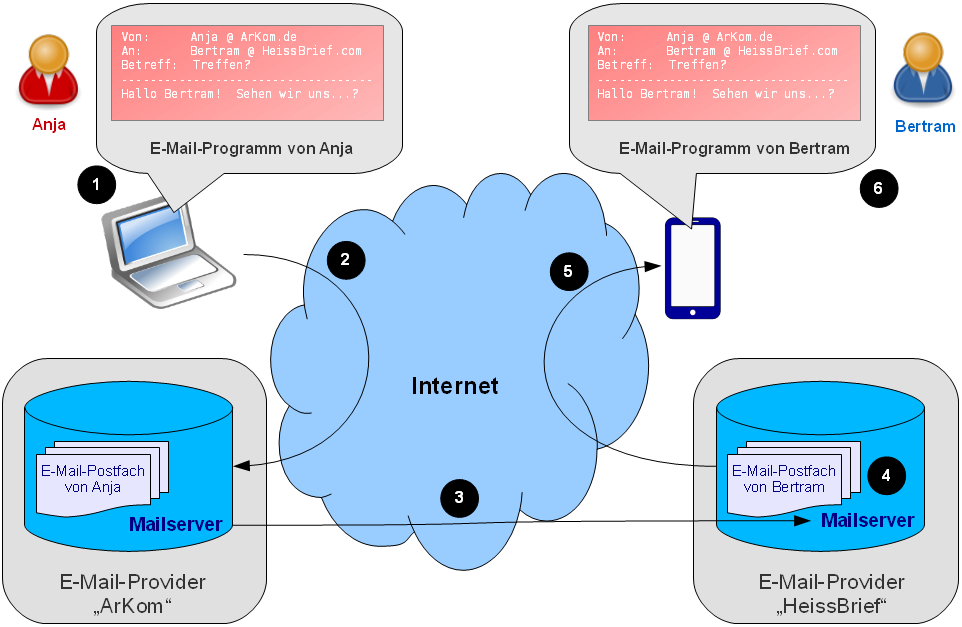
\includegraphics[scale=0.6]{../docs/lyaton/graphics/E-Mail-Prinzip.png}\\
\textbf{Abstraktes Prinzip - Zustellung einer E-Mail}\\
\begin{scriptsize}
Bearbeitetes Bild - Quelle: http://de.wikipedia.org/wiki/E-Mail\#/media/File:E-Mail-Prinzip-v05.png
\end{scriptsize}
\end{center}
\vspace{0.5cm}

Das obige Bild beschreibt auf abstrakte Weise das Prinzip der Zustellung einer E-Mail. Es ist in 6 Teilsegmenten aufgeteilt, die im Folgenden erklärt werden.

\begin{enumerate}
\item Anja hat mit ihrem E-Mail Programm eine E-Mail erstellt. In dieser E-Mail können der Absender (Von: Anja@Arkom.de), der Empfänger (An:Bertram@HeissBrief.com), der Betreff (Betreff: Treffen?) und der Inhalt (Hallo Bertram! Sehen wir uns...?) erkannt werden. Anja sendet ihre Nachricht ab.\\\\
Ab hier übernimmt das E-Mail Programm von Anja, d.h. Anja muss sich nicht mehr um die E-Mail kümmern.
\item Anjas E-Mail Programm hat dafür gesorgt, dass Arkom,  Anjas E-Mail Provider, die abzusendende E-Mail bekommt. Ab hier übernimmt der Mailserver von Arkom.
\item In diesem Schritt sendet Arkom, die E-Mail an den Mailserver von HeissBrief, Bertrams E-Mail Provider.
\item HeissBrief speicher die E-Mail auf dem Server gespeichert und weißt diese Bertrams Postfach zu. Sie kann jederzeit bei Bedarf abgerufen werden.
\item In Folgendem Schritt, überprüft Bertrams E-Mail Programm, ob sich neue E-Mails in seinem Postfach befinden. Da dies der Fall ist wird es die neue E-Mail herunterladen und ihm mitteilen, dass er eine neue E-Mail bekommen hat.
\item Schlussendlich kann die E-Mail gelesen werden.
\end{enumerate} 

\subsection{Aufbau}
Der allgemeine Aufbau einer E-Mail wird in zwei Teile gegliedert:
\begin{enumerate}
\item Header\\
Dieser beinhaltet Informationen über:
\begin{itemize}
\item Absender
\item Empfänger und eventuelle zu sendende Kopien
\item eventuellen Betreff
\item eventuellen Anhang
\item weitere formelle Informationen...
\end{itemize}
\item Body\\
Der Body beinhaltet die eigentliche Nachricht
\end{enumerate} 
\subsubsection{Header}
\begin{center}
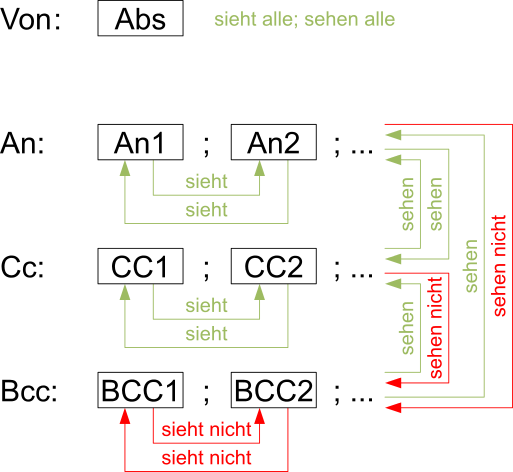
\includegraphics[scale=0.9]{../docs/lyaton/graphics/E-Mail-Header.png}\\
\textbf{E-Mail Header}\\
\begin{tiny}
Konvertiertes Bild - Quelle:\\http://de.wikipedia.org/wiki/Header\_(E-Mail)\#/media/File:FromToCcBCC-Who\_sees\_what.svg
\end{tiny}
\end{center}
\vspace{0.5cm}
Der Header, ist wieder im Vergleich mit der Post, das Briefkuvert. Er enthält das für das Versenden notwendige Informationsmaterial. Im Gegensatz zu anderen Nachrichtensystemen ist es bei E-Mails möglich, eine Nachricht an mehrere Empfänger gleichzeitig zu senden.\\
Wie man im obigen Bild gut erkennt, können Empfänger sogar speziellen Ranglisten bzw. Rangstufen zugeordnet werden:
\begin{itemize}
\item CC - Carbon Copy\\
Sie werden auch oft als 'Courtesy Copy' bezeichnet, was soviel bedeutet wie Höflichkeits-Kopie. Sie wird dazu verwendet, um Hauptempfänger ganz klar von eventuellen Nebenempfängern zu unterscheiden. Solche Nebenempfänger sind z.B. Leute, die nur zur Kenntnis nehmen sollen, dass jene E-Mail versendet wurde oder Leute die auch diese E-Mail bekommen sollten, Beispielsweise wäre ein solcher Nebenempfänger die Buchhaltung beim elektronischen Versandt einer Rechnung.
\item BCC - Blind Carbon Copy\\
Diese Stufe wird verwendet, um Leute, die von den anderen Empfängern nicht gesehen werden dürfen, hinzuzufügen. Sie wird zum Schutz der Privatsphäre mitunter beim versenden von Rundmails gebraucht. 
\end{itemize}  
Die Pfeile in der obigen Abbildung 'E-Mail Header' zeigen übersichtlich die Visibilität aller Beteiligten untereinander.
\subsection{Senden}
Zum Senden einer E-Mail, wird ein relativ altes Protokoll verwendet, namens SMTP. Es wird weitgehend auf SMTP bzw. seine Weiterentwicklungen zurückgegrifen, da es kaum Alternativen gibt.
\subsubsection{SMTP - Simple Mail Transfer Protocol}
Wie bereits vorher erwähnt, wird dieses Protokoll zum Versenden von E-Mails verwendet.\\\\ 
Eigenschaften:\\
\begin{itemize}
\item Port:
\begin{itemize}
\item 25/TCP
\item 465/TCP\\
für SMTPS (SMTPSecure unterscheidet sich insofern, dass anfänglich eine Verschlüsselung (siehe Kapitel \ref{chap:krypto} Seite \pageref{chap:krypto}) zwischen Client und Server ausgemacht wird.)
\item 587/TCP\\
für Mail-Clients (bzw. E-Mail Programm)
\end{itemize}
\item Netzwerklayer: Anwendung
\item Dokumentation: RFC 5321 (Ursprünglich 821)
\end{itemize}
\paragraph{Allgemein - Sendevorgang\\\\}
Um den Sendevorgang verständlicher zu machen, müssen vorerst einige Fachbegriffe näher erklärt werden.
\begin{itemize}
\item MUA - Mail User Agent\\\label{itm:MUA}
Der Mail User Agent bildet die Schnittstelle zwischen Benutzer und System und ist somit von großer Bedeutung. Es gibt unzählige Anbieter für einen solchen Agent. Es ist ein Programm, das graphisch so aufbereitet wurde, dass es dem Benutzer auf komfortable Art und Weise ermöglicht mit dem System zu interagieren. Der Mail User Agent sorgt sowohl für das Senden als auch da Empfangen einer E-Mail.\\\\
Web-Applikationen wie zum Beispiel 'Outlook.com' oder 'Gmail', werden zwar e webmail-Systeme (Web-basierender E-Mail Client) angesehen, stellen im Prinzip aber auch Mail User Agents dar.
\item MSA - Mail Submission Agent\\\label{itm:MSA}
Der Mail Submission Agent bildet eine Vorstufe zum Mail Transfer Agent (im nächsten Punkt erklärt). Ein Mail Submission Agent ist kein Muss, denn seine Aufgaben können auch vom Mail Transfer übernommen werden, jedoch gibt es ein paar Vorteile die für den Einsatz von Mail Submission Agents sprechen:
\begin{itemize}
\item Der MSA stellt sozusagen einen Vorfilter dar. D.h. falls der Benutzer eine E-Mail nicht formgerecht (kein Datum angegeben, keine Empfängeradresse angegeben) abgesendet hat, dann sendet der MSA sofort eine Fehlermeldung. Dadurch kann die E-Mail vom Benutzer schnell nachbearbeitet und erneut abgesendet werden. Für gewöhnlich jedoch, fängt die MUA solche Fehler ab. Nichtsdestotrotz ist es sinnvoll zur Sicherheit eine MSA zu implementieren, denn falls die MTA darauf reagieren müsste, würde die Fehlermeldung den Benutzer, falls überhaupt, meist viel zu spät erreichen.
\item Die meisten MSAs verlangen eine Benutzerauthentifizierung, damit genau protokolliert werden kann, wer, wem und wann eine E-Mail gesendet hat. Absender, die Spam-Traffic verursachen können somit relativ schnell ausfindig gemacht werden (siehe Kapitel \ref{sssec:Spam} Seite \pageref{sssec:Spam}). 
\end{itemize}
\item MTA - Mail Transfer Agent\\\label{itm:MTA}
Dieser bildet den Kern des Sendevorganges. Er sorgt dafür, dass die E-Mails, die entweder direkt von MUAs oder von MSAs an ihn gesendet wurden, ihren Weg zum MTA bzw. MDA (im nächsten Punkt erklärt) des Empfängers finden.
\item MX Record\\\label{itm:MX Record}
Der MX Record enthält die für den Sendevorgang notwendigen Informationen:
\begin{itemize}
\item Präferenz
\item Mail Exchanger Adresse
\end{itemize}
Der MX-Record sieht so aus:
\begin{center}
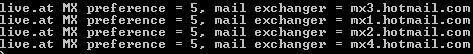
\includegraphics[scale=1]{../docs/lyaton/graphics/MX-Record.png}\\
\textbf{MX Record Lookup}
\end{center}
Die Präferenz ist deshalb von Bedeutung, da sowohl viele Firmen als auch manche Privatpersonen mehr als nur einen Mail Exchanger (Im nächsten Punkt erklärt) haben. Die Präferenz stellt also die Priorität dar, mit welcher ein Mail Exchanger angesprochen werden. Je kleiner die Zahl der Präferenz desto höher ist die Priorität. (Im obigen Bild ist viermal die gleiche Zahl als Präferenz angegeben. Diese Methode wird angewendet, um alle verfügbaren Server gleichmäßig auszulasten.)
\item MX - Mail Exchanger\\\label{itm:MX}
Nachdem der MTA des Absenders die Empfängeradresse kennt, leitet er die E-Mail dessen Mail Exchanger weiter. Somit stellt der MX den ersten Server des Empfängers dar, mit dem die E-Mail Kontakt hat. 
\item MDA - Mail Delivery Agent\\\label{itm:MDA}
Der MDA sorgt für die Zuweisung der jeweiligen E-Mails zu den richtigen Benutzerkonten. Er ist jener Server, den der MUA des Empfängers anspricht, um die Mails abzurufen.
\end{itemize}
\begin{center}
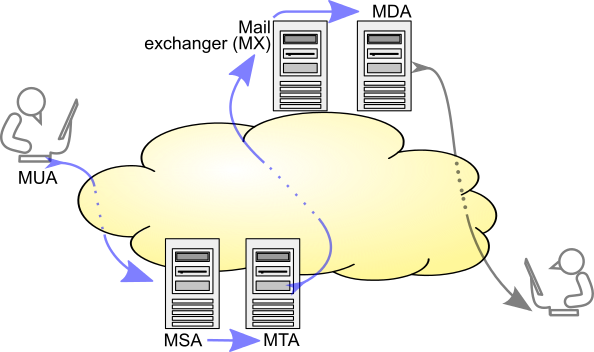
\includegraphics[scale=0.5]{../docs/lyaton/graphics/SMTP-Uebertragung.png}\\
\textbf{SMTP-Übertragung}\\
\begin{scriptsize}
Konvertiertes Bild - Quelle:\\
http://en.wikipedia.org/wiki/Simple\_Mail\_Transfer\_Protocol\#/media/File:SMTP-transfer-model.svg
\end{scriptsize}
\end{center}
Im Folgenden werden die einzelnen Schritte von der obigen Abbildung näher erläutert. 
\begin{enumerate}
\item Erstellvorgang und Absendevorgang einer E-Mail des MUAs\\
Am Beginn steht der  Autor der E-Mail, welcher seine Nachricht über den MUA schreibt und sie absendet (siehe Kapitel \ref{itm:MUA} Seite \pageref{itm:MUA}).
\item MUA $\rightarrow$ MSA (MSA siehe Kapitel \ref{itm:MSA} Seite \pageref{itm:MSA})\\
In manchen Fällen fällt dieser Schritt weg, da der MTA diese Aufgabe weitgehend übernimmt (siehe Kapitel \ref{itm:MTA} Seite \pageref{itm:MTA}).\\\\
Der MSA überprüft die E-Mail darauf, ob sie vollständig ist und leitet sie weiter zum MTA.
\item MTA $\rightarrow$ MX  (siehe Kapitel \ref{itm:MX} Seite \pageref{itm:MX})\\
Dieser Schritt besteht aus einigen wichtigen Teilschritten:
\begin{enumerate}
\item Wenn die E-Mail in Ordnung ist, ließt der MTA den Hostnamen (siehe Kapitel \ref{sssec:Entstehung} Seite \pageref{sssec:Entstehung}) des Empfängers aus dessen E-Mail Adresse aus. Mit dem Hostnamen kann er beim DNS (siehe Kapitel \ref{ssec:DNS} Seite \pageref{ssec:DNS}) den MX-Record (siehe Kapitel \ref{itm:MX Record} Seite \pageref{itm:MX Record}) des Hostservers in Erfahrung bringen.
\item Mit der im MX-Record stehenden Mail Exchanger Adresse wird nochmals beim DNS angefragt, , diesmal jedoch für den A- und/oder AAAA-Record.  Dieser enthält die IP-Adresse (siehe Kapitel \ref{sssec:ipaddr} Seite \pageref{sssec:ipaddr}) des MXs, damit ist geklärt wohin die E-Mail gesendet werden muss.
\item Als nächstes erfolgt die Übergabe der E-Mail. Der Mailserver des Absenders übergibt die E-mail dem Mailserver des Empfängers. 
\end{enumerate}
\item MX $\rightarrow$ MDA (siehe Kapitel \ref{itm:MDA} Seite \pageref{itm:MDA})\\
Dies ist der letzte Schritt des Sendevorganges. Der MX des Empfänger sendet die E-Mail weiter an den MDA. Der MDA stellt in diesem fall das Postfach dar.
\end{enumerate}
Die E-Mail ist im Postfach des Empfängers abgespeicher und wartet darauf 'empfangen' zu werden. 
\paragraph{Befehle\\}
Die Grundbefehle einer STMP - Kommunikation:
\begin{itemize}
\item HELO\\
HELO eröffnet die Sitzung am Server.
\item EHLO\\
EHLO eröffnet die Sitzung und identifiziert den Client eindeutig am Server mit einer Passwortabfrage.
\item MAIL FROM\\
Mit MAIL FROM kann die Absender Adresse hinzufügt werden (falls EHLO verwendet wird, ist dieser Schritt überflüssig).
\item RCPT\\
RCPT fügt Empfänger hinzu. Außerdem ist die multiple Anwendung dieses Befehls möglich, um mehrere Empfänger anzugeben. 
\item DATA\\
DATA signalisiert den dem Server, dass als nächstes die E-Mail-Nachricht versendet wird. \\
(Das Ende einer Nachricht ist eine Zeile die nur einen Punkt enthält.) 
\item RSET\\
Mit RSET wird die bisherige Übertragung zurückgesetzt bzw. gelöscht. Die Verbindung zwischen Client und Server bleibt allerdings weiterhin bestehen.
\item VRFY\\
Mit VRFY kann überprüft werden ob die Empfänger-Adresse existiert.
\item EXPN\\
EXPN ist für mache MTAs (siehe \ref{itm:MTA} Seite \pageref{itm:MTA}) der Befehl für VRFY.
\item NOOP\\
NOOP ist quasi ein 'Lebenszeichen' des Clients an den Server um die Verbindung aufrechtzuerhalten. Andernfalls würde diese, aufgrund eines Timeouts getrennt werde.
\item QUIT\\
QUIT trennt die Verbindung zum Server. Der Server sendet jedoch noch eine letzte Trennungsbestätigung.
\end{itemize}
\newpage
Eine SMTP Kommunikation kann beispielsweise wie folgt aussehen:
\begin{center}
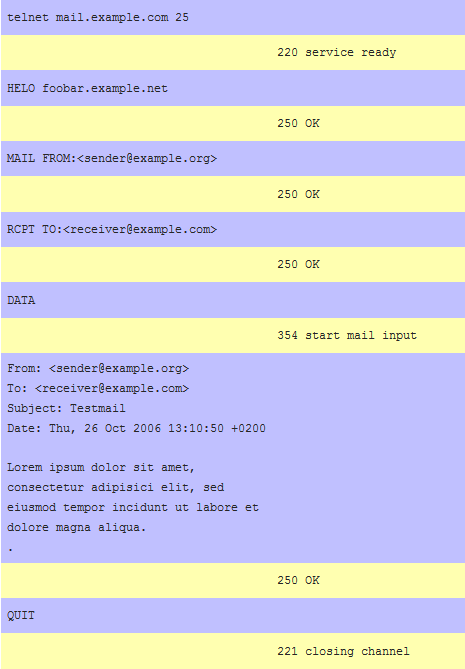
\includegraphics[scale=0.9]{../docs/lyaton/graphics/SMTP-Kommunikation.png}\\
\textbf{SMTP - Kommunikation}\\
\begin{scriptsize}
Quelle: http://de.wikipedia.org/wiki/Simple\_Mail\_Transfer\_Protocol
\end{scriptsize}
\end{center}
Die obigen Abbildung beschreibt folgende Schritte:

\begin{enumerate}
\item \textbf{Client:} Die Verfügbarkeit wird mithilfe einer TELNET-Anfrage, an Mail.example.com über Port 25, geprüft.\\\\
\textbf{Server:} Dieser zeigt die Verfügbarkeit an. 
\item \textbf{Client:} Es wird um eine Sitzungseröffnung angefragt. \\\\
\textbf{Server:} Der Server bestätigt die Sitzungseröffnung. 
\item \textbf{Client:} Der Client fügt den Absender hinzu (sender@example.org).\\\\
\textbf{Server:} Diese wird im Anschluss vom Server bestätigt. 
\item \textbf{Client:} Es wird auch der Empfänger hinzugefügt (receiver@example.com).\\\\
\textbf{Server:} Der Server bestätigt dieses wiederum. 
\item \textbf{Client:} Im Anschluss muss signalisiert werden, dass die E-Mail zum Versand bereit ist. \\\\
\textbf{Server:} Es wird ein Startsignal für das Senden der E-Mail verschickt.
\item \textbf{Client:} Als nächstes muss die E-Mail gesendet werden. \\
(From: <sender@example.com>\\
To: <receiver@example.com>\\
Subject:......
.\\
)\\\\
\textbf{Server:} Der Server bestätigt den Empfang der Nachricht. 
\item \textbf{Client:} Es wird um die Trennung der Verbindung angefragt.\\\\
\textbf{Server:} Zuletzt wird durch den Server die Trennung der Verbindung bestätigt.
\end{enumerate}
\subsection{Empfangen}
Der Empfang einer E-Mail kann einerseits über IMAP andererseits über POP geleitet werden. 
\subsubsection{IMAP - Internet Message Access Protocol}
Eigenschaften:\\
\begin{itemize}
\item Port:
\begin{itemize}
\item 143/TCP
\item 993/TCP\\
für IMAPS (IMAPSecure unterscheidet sich vom IMAP durch die anfängliche Verschlüsselung. Diese wird zwischen Client und Server beschlossen. (siehe Kapitel \ref{chap:krypto} Seite \pageref{chap:krypto}))

\end{itemize}
\item Netzwerklayer: Anwendung
\item Dokumentation: RFC 3501
\end{itemize}
Es existieren mehrere Versionen von IMAP. Die Version IMAP 4 wird heutzutage noch immer verwendet obwohl sie aus den 1990er Jahren stammt. 
\paragraph{Allgemeine Funktionsweise\\}
IMAP ermöglicht den Zugriff auf ein E-Mail Konto. Hierbei bleiben die E-Mails jedoch auf dem Server und werden von den Clients nur in den temporären Speicher geladen. Sie können dort weiter sortiert und durchsucht werden. \\

Hier bestehen Vor- aber auch Nachteile, die in der Gegenüberstellung (siehe Kapitel \ref{sssec:IMAPvsPOP} Seite \pageref{sssec:IMAPvsPOP}) näher erläutert werden\\\\
Die folgende Abbildung zeigt eine mögliche IMAP-Kommunikation zwischen Client und Server.\\
\begin{center}
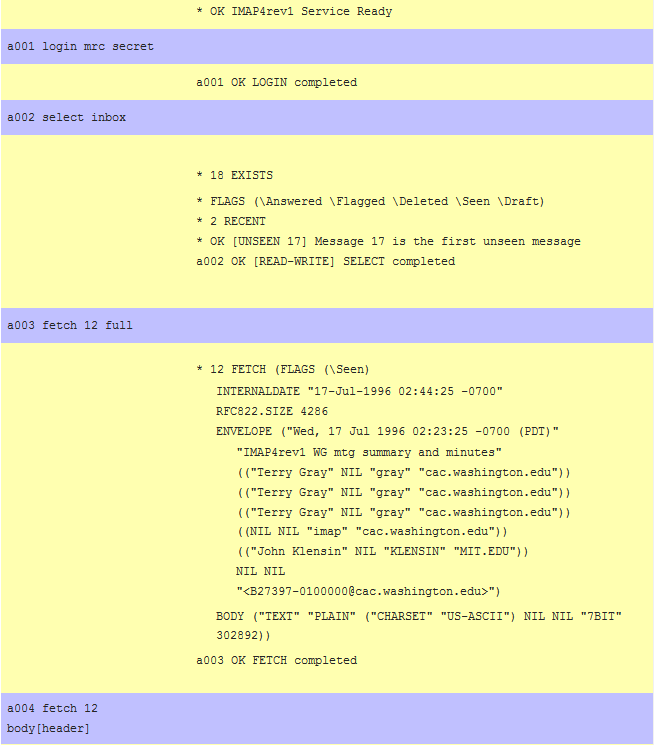
\includegraphics[scale=0.7]{../docs/lyaton/graphics/IMAP-Kommunikation_p1.png}
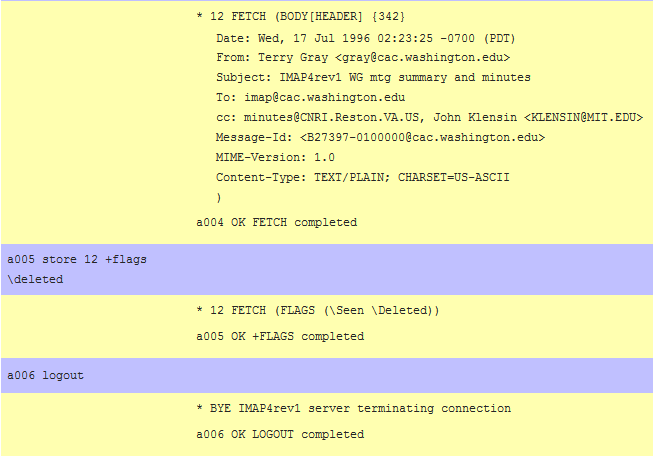
\includegraphics[scale=0.7]{../docs/lyaton/graphics/IMAP-Kommunikation_p2.png}\\
\textbf{IMAP - Kommunikation}\\
\begin{scriptsize}
Quelle: http://de.wikipedia.org/wiki/Internet\_Message\_Access\_Protocol\#Geschichte
\end{scriptsize}
\end{center}

Die obige Abbildung zeigt folgende Schritte an: 
\begin{enumerate}
\item \textbf{Server:} Der Server hört auf den Port und wartet auf eventuelle Anfragen.\\\\
\textbf{Client:} Es wird eine Anmeldungsanfrage versandt.
\item \textbf{Server:} Dieser bestätigt die Anmeldung.\\\\
\textbf{Client:} Der Client wählt einen Ordner aus (Inbox). 
\item \textbf{Server:} Es wird eine Übersicht des Ordners versendet.\\\\
\textbf{Client:}  Eine Information über Email Nr.12 wird vom Client gefordert.
\item \textbf{Server:} Der Server wiederum versendet Informationen über E-Mail Nr. 12. \\\\
\textbf{Client:} Daraufhin fordert der Client einen Header. 
\item \textbf{Server:} Es wird der gewünschte Header versandt. \\\\
\textbf{Client:} Der Client möchte die E-Mail Nr. 12 löschen.
\item \textbf{Server:} dieser Löschvorgang muss vom Server bestätigt werden.\\\\
\textbf{Client:} Es wird um Abmeldung angefragt.
\item \textbf{Server:} Abermals muss eine Bestätigung der Anfrage verschickt werden.
\end{enumerate}
\subsubsection{POP - Post Office Protocol}
Eigenschaften:\\
\begin{itemize}
\item Port:
\begin{itemize}
\item 110/TCP
\item 995/TCP\\
für POPS (POPSecure unterscheidet sich vom POP durch die anfängliche Verschlüsselung. Diese wird zwischen Client und Server beschlossen.  (siehe Kapitel \ref{chap:krypto} Seite \pageref{chap:krypto}))

\end{itemize}
\item Netzwerklayer: Anwendung
\item Dokumentation: RFC 1939
\end{itemize}
Das Post Office Protocol ist eine weitere Möglichkeit um E-Mails vom Mailserver abzurufen. Auch hier gibt es mehrere Versionen, wobei POP3 aktuell verwendet wird. Das POP3 erschien erstmals im Jahre 1988 und ist somit ein relativ altes, jedoch intaktes Protokoll.
\paragraph{Allgemeine Funktionsweise\\}
POP ermöglicht es die E-Mails vom Mailserver auf ein lokales Speichermedium zu laden und speichern. Damit können E-Mails, ohne notwendige Verbindung zum Server, lokal verwaltet werden. \\

Auch hier bestehen sowohl Vor- als auch Nachteile. Diese werden in der Gegenüberstellung (siehe Kapitel \ref{sssec:IMAPvsPOP} Seite \pageref{sssec:IMAPvsPOP}) näher erläutert.\\\\
Mögliche POP Kommunikation zwischen Client und Server:\\
\begin{center}
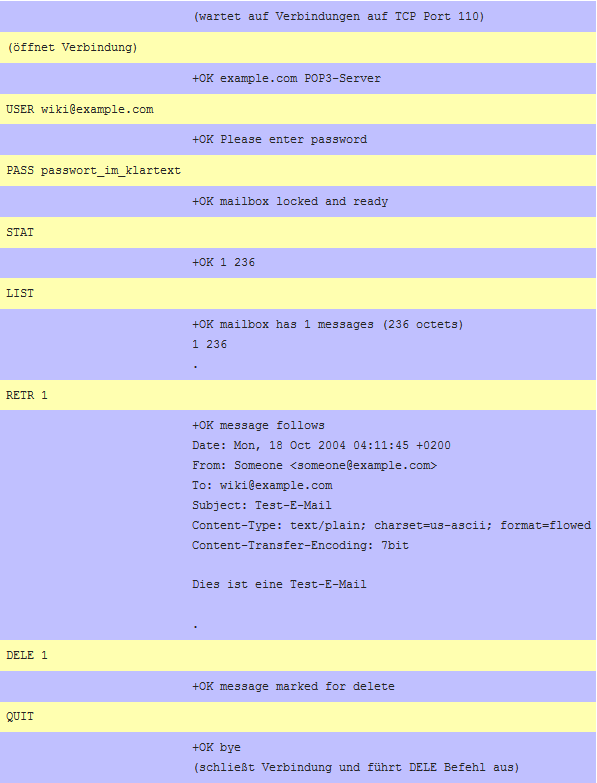
\includegraphics[scale=0.7]{../docs/lyaton/graphics/POP-Kommunikation.png}\\
\textbf{POP - Kommunikation\\}
\begin{scriptsize}
Quelle: http://de.wikipedia.org/wiki/Post\_Office\_Protocol
\end{scriptsize}
\end{center}

Im Folgenden werden die einzelnen Schritte von der obigen Abbildung näher erläutert: 
\begin{enumerate}
\item \textbf{Server:} Der Server hört auf den Port und wartet auf eventuelle Anfragen.\\\\
\textbf{Client:} Es wird eine Anfrage ausgesendet. 
\item \textbf{Server:} Der Server bestätigt die Anfrage und zeigt somit, dass er aktiv ist.t\\\\
\textbf{Client:} Der Client gibt seinen Benutzernamen durch.
\item \textbf{Server:} Es wird nach dem Passwort verlangt.\\\\
\textbf{Client:} Das verlangte Passwort wird vom Client durchgegeben. 
\item \textbf{Server:} Die Anmeldung wird bestätigt.\\\\
\textbf{Client:} Der Client fragt den aktuellen Status ab.
\item \textbf{Server:} Der Server versendet den angeforderten Status.\\\\
\textbf{Client:} Es wird eine Auflistung gefordert. 
\item \textbf{Server:} Eine aktuelle Liste der E-Mails wird versandt. \\\\
\textbf{Client:} Der Client fragt die E-Mail Nr. 1 ab.
\item \textbf{Server:} Der Server sendet dem Clienten die E-Mail Nr.1 komplett zu. \\\\
\textbf{Client:} Es wird die E-Mail Nr.1 zum löschen markiert.
\item \textbf{Server:} Dieser Löschvorgang muss wiederum vom Server bestätigt werden.\\\\
\textbf{Client:} Der Client meldet sich ab. 
\item \textbf{Server:} Der Server löscht im Anschluss die E-Mail und bestätigt die Abmeldung. \\\\
\end{enumerate}

\subsubsection{Gegenüberstellung IMAP - POP} \label{sssec:IMAPvsPOP}
IMAP und POP sind Protokolle, die heutzutage unter Verwendung stehen, wobei POP etwas verbreiteter ist. Beide haben sowohl ihre Vor- als auch Nachteile. \\\\
\begin{center}
\begin{tabular}{p{6cm}|c|p{6cm}}
\textbf{IMAP} & vs. &\textbf{POP}\\
\hline
Alle Nachrichten werden auf dem Server gespeichert und lokaler Speicher wird kaum benötigt. & $\leftarrow$ & Abgerufene E-Mails werden zusätzlich auf dem lokalem Speicher gesichert und sind in diesem Fall doppelt vorhanden. \\
\hline
Die Zeit bis eine bestimmte E-Mail gelesen werden kann ist sehr kurz. & $\leftarrow$ & Der Zeitaufwand bei einem POP ist durch die Ladezeit verlängert. \\
\hline
Server und MUA (siehe Kapitel \ref{itm:MUA} Seite \pageref{itm:MUA}) sind immer synchron. & $\leftarrow$ & Alle E-Mails werden von dem MUA lokal verwaltet, dadurch kann es zu keiner Synchronisation zwischen MUA und MDA kommen.  (siehe Kapitel \ref{itm:MDA} Seite \pageref{itm:MDA}).\\
\hline
Server werden stark belastet, da alles online verwaltet wird. & $\rightarrow$ & Durch die lokale Verwaltung werden die Server nicht ausgelastet.\\
\hline
Eine durchgehende Verbindung zum Server ist notwendig & $\rightarrow$ & Da die E-Mails lokal gespeichert werden, ist die Verbindung zum Server nur während des Downloads notwendig.
\end{tabular}
\end{center}
\paragraph{IMAP und POP im Vergleich mit der Post:}
\subparagraph{IMAP:} IMAP: Die Post wird direkt am Briefkasten gelesen und vom Briefkasten nach Belieben sortiert und entsorgt.
\subparagraph{POP:} POP: Die Post wird direkt am Briefkasten entsorgt oder kopiert. Die Kopien können mit nach Hause genommen werden. Dort können sie gelesen und verwaltet werden. 
\section{Bedeutung im Alltag}
\begin{flushright}
\begin{tiny}
Quellen: [302]
\end{tiny}
\end{flushright}
\subsubsection{Heute}
E-Mails sind heute eine der meistgenutzten Kommunikationsmöglichkeiten überhaupt. Vor allem Firmen senden massenhaft E-Mails. Die elektrische Post ist aus dem heutigen Alltag kaum mehr wegzudenken.\\\\
Viele Geräte unterstützen diese Technik, wie z.B. Smartuhren, Smartphones, Tablets, Laptops, und viele mehr. Dadurch wird die schnelle Abrufbarkeit gewährleistet.
\paragraph{Nennenswerte E-Mail Anbieter sind:}
\begin{itemize}
\item GMAIL
\item Outlook
\item GMX
\item Yahoo
\item uvm.
\end{itemize} 
\subsubsection{Zukünftig}
Analysten zufolge wird der E-Mail-Verkehr sich immer mehr in den wirtschaftlichen Sektor verschieben, da die Menschen immer mehr ihre Sozialen Kontakte über soziale Netwerke, wie Facebook, Whatsapp und Twitter aufrecht erhalten. E-Mails zwischen zwei Freunden werden voraussichtlich immer seltener. (vgl.http://de.wikipedia.org/wiki/E-Mail)
\section{Probleme}
\begin{flushright}
\begin{tiny}
Quellen: [303]
\end{tiny}
\end{flushright}
Beim Versand von E-Mails gibt es nach wie vor auch einige Probleme, die schwer zu bewältigen sind. Dieses sind z.B. Spam und Informations-Overloads. Auf einige bekannte Probleme wird im folgenden eingegangen.
\subsection{Begrenzungen}
E-Mails könnten zwar rein theoretisch unbegrenzte Datenmengen übertragen, dies ist jedoch in der Praxis nicht umsetzbar. Viele Betreiber von Mailservern limitieren die Datenmengen um die Auslastung so gering wie möglich zu halten. 
\subsection{Informations-Overload}
Jeder empfängt unzählige E-Mails. Diese variieren von wichtigem Informationsaustausch, über überflüssige Werbung, bis zu gefährlichen E-Mails. Zwangsweise führt dies zu einer Informationsüberflutung. 
\subsection{Spam}\label{sssec:Spam}
Als Spam werden jene E-Mails bezeichnet, welche meist einen werbenden Inhalt haben. 2010 lag der Prozentsatz von Spam-Mails bei knapp 90\%, bei 107 Billionen versendeten E-Mails weltweit.  (vgl.http://de.wikipedia.org/wiki/E-Mail\#Spam) 
\chapter{Schnittstellen (Alin Porcic / Manpreet Singh)}

\section{Command Line Interface (Alin Porcic)}
\lfoot{Alin Porcic}
\subsection{Allgemeines}

CLI steht für \textbf{Command Line Interface} (=textbasierende Schnittstelle) und darunter versteht man Schnittstellen, die für die Interaktion mit Programmen zeilenweise Befehle in Form von Text einlesen, interpretieren und anschließend ausführen. Programme, die solche Schnittstellen anbieten, werden \textbf{CLI-Interpreter} genannt. Der Begriff \textbf{Shell} hat sich unter unixähnlichen Betriebssystemen als eine andere Bezeichnung für einen CLI-Interpreter eingebürgert. Bekannte CLI-Interpreter sind zum Beispiel: \textbf{sh}, \textbf{bash} oder \textbf{Windows PowerShell}. [100] [102]

\begin{center}
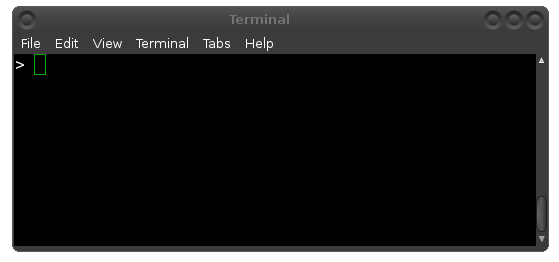
\includegraphics[scale=0.5]{img/cli_pic.png}\\
der Terminalemulator 'Xfce-Terminal' mit Bash
\end{center}

\begin{center}
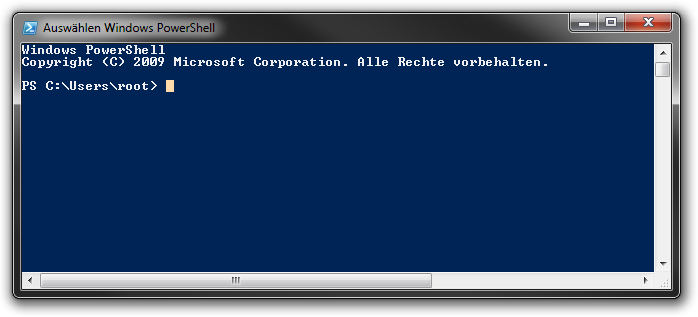
\includegraphics[scale=0.52]{img/powershell.png}\\
Windows Powershell
\end{center}

Bei unixähnlichen Betriebssystemen wird der Begriff \textbf{Terminal} häufig mit CLI in Verbindung gebracht. Ein Terminal (oder auch Konsole) war ein Gerät, das die Eingaben und Ausgaben von Daten aufgit einem Computer in Textform ermöglichte. Da diese Geräte heute eher störend und nutzlos sind, werden sie in Software emuliert, daher spricht man auch von \textbf{Terminalemulatoren}. Die Hauptaufgaben von diesen Emulatoren sind die richtige Darstellung der Textkodierung, die Darstellung von Farben, das Erkennen von Escape-Sequenzen und das Einlesens von Eingaben - die CLI hingegen, ist für die vollständige Interpretation sowie der Ausführung zuständig. [101]\\

Grundsätzlich wurden die textbasierten Schnittstellen im Desktop-Bereich von den graphischen Schnittstellen abgelöst, dennoch werden bei vielen Systemen auch alternative Schnittstellen, wie eine CLI, angeboten. Vorallem im Netzwerkbereich sind textbasierte Schnittstellen durch ihre enorme Flexibilität und ihren minimalen Ressourcenverbrauch immer noch häufig anzutreffen (z.B. pfSense, Cisco-Router/Switches). Die primäre Kommunikation mit unixähnliche Betriebssystemen hat sich bis heute nicht geändert und erfolgt immer noch über Kommandozeileninterpreter. Bei diesen Systemen ist die CLI ein fester Bestandteil, die Interaktion basiert fast ausschließlich über die textbasierte Schnittstelle, grafische Oberflächen hingegen, sind meist nur optioanle Zusatzsoftware. [102]\\ 

Erfahrene Nutzer greifen auch heute immer noch zu Kommandozeileninterpreter, da sie eine schnellere und direkte Kontrolle über die Ausführung von Programmen haben. Zudem besteht die Möglichkeit Programme mithilfe von \textbf{Scripts} zu kombinieren oder die Ausgaben von Programmen in anderen zu leiten. [103]

\subsection{Geschichte}

Die aller ersten Computer unterstützten keine Interaktiven Eingabe- oder Ausgabegeräte und daher war die Überwachung von Programmen nur mithilfe von Kontrolllampen und Schaltern möglich. Ab 1960 wurden die textbasierten Schnittstellen für die Interaktion eingeführt. Die Befehle für diese textbasierten Schnittstellen konnten mithilfe von Fernschreibern, wie der \textbf{Teletype Model 33 ASR}, auf Lochkarten gestanzt werden und von der Schnittstelle eingelesen, interpretiert und ausgeführt werden. [104] [105]\\

\begin{center}
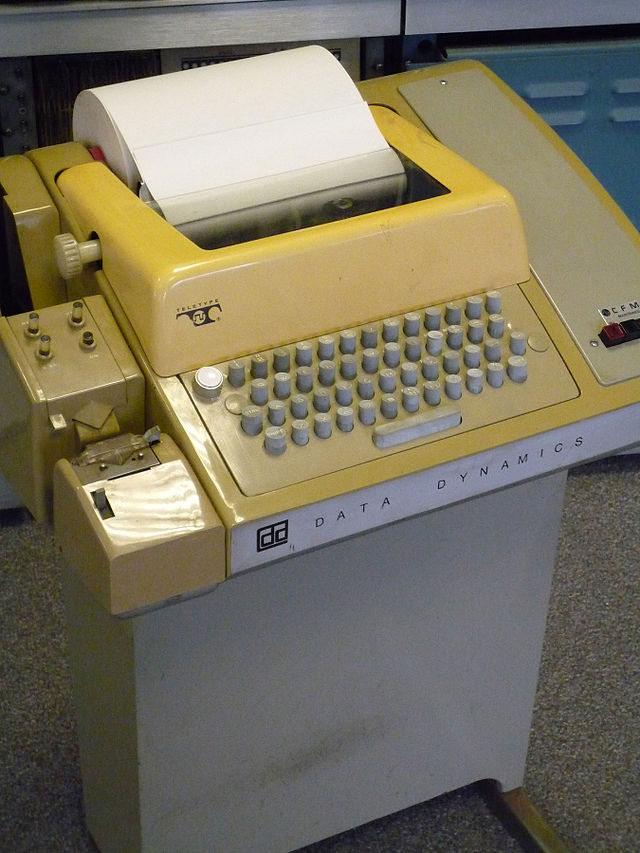
\includegraphics[scale=0.52]{img/teletype.jpg}\\
Teletype Model 33 ASR (Quelle: [105])
\end{center}

Anfangs der 1970er Jahre begann das Unternehmen Bell Labs die Entwicklung eines Betriebssystems namens \textbf{Unix}. Unix besaß eine mächtige CLI-Umgebung und konnte durch sogenannte \textbf{Pipes} die Ausgaben von Programmen umleiten. Es gab auch die Möglichkeit mehrere Programmanweisungen in ein Script zu verpacken und auszuführen. \\

Die Fernschreiber waren sehr ümständlich, da die Instruktionen erst gestanzt und dann vom Computer eingelesen werden mussten. Daher entwickelte man die Terminals, um die Fernschreiber zu erlösen. Terminals waren Geräte, die die Möglichkeit boten, Daten über eine Tastatur einzugeben und die Daten über einen Bildschirm in Textform oder auch Grafik auszugeben. Zudem boten die Termianls durch die serielle Verbindung mehr Bandbreite und konnten einfacher in ein Unternehmen eingesetz werden. Das VT100 war ein ASCII-Computer-Terminal, dass zwischen 1979 bis 1983 verkauft wurde.\\

\begin{center}
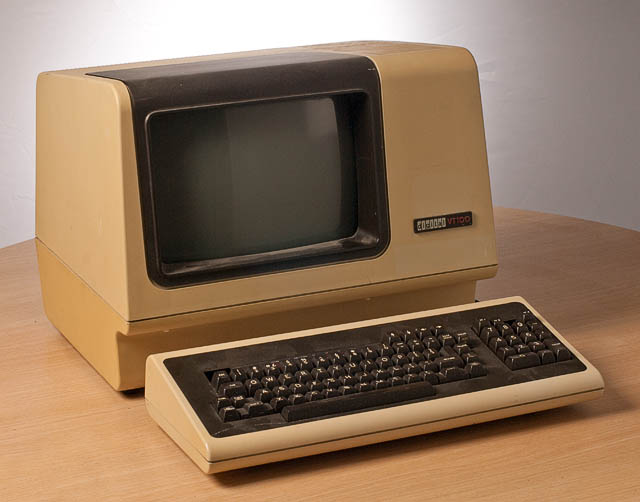
\includegraphics[scale=2.0]{img/vt100.jpg}\\
VT100 (Quelle: http://de.wikipedia.org/wiki/VT100)
\end{center}

Die Terminals wurden jedoch schon 1977 durch den Einsatz von \textbf{Personal Computer} ersetzt. Seitdem werden richtige Terminals nicht mehr eingesetzt, sondern werden in Software emuliert. [101]\\

Obwohl der Einsatz von textbasierten Schnittstellen nachgelassen hat, finden sie immer noch große Verwendung. Einige Betriebssysteme (Windows, Mac OS, ...) und auch einige Programme (QEMU, CodeBlocks, Eclipse, ...) bieten neben ihren graphischen Oberflächen auch alternative textbasierte Schnittstellen an. Bei \textbf{Embedded Systems} werden auch häufig auf CLIs zurückgegriffen, da sie sehr Ressourcen freundlich sind, aber auch Router und Switches machen sich die Vorteile der CLI zu nutze. [102]

\subsection{Vor- und Nachteile}

In CLI-Anwendungen lassen sich viel mehr Einstellungen vornehmen als bei grafischen Anwendungen. Ein gutes Beispiel hierführ ist der C/C++ Compiler 'gcc'. Eine grafische Oberfläche für die Benutztung dieses Compilers müsste über enorm viele Einstellungen und Textfelder verfügen, um die Möglichkeit zu bieten, den Compiler bis ins Detail zu konfigurieren. Da die Umsetzung einer Oberfläche für den 'gcc' sehr schwierig ist, werden in modernen IDEs einfach ein CLI-Interpreter eingebaut, der für die Verwendung des Compilers verwendet werden kann.\\

CLI sind sehr Ressourcen freundlich und können daher auf sehr leistungsschwachen Systemen einwandfrei verwendet werden. Außerdem ist es mit Protokollen, wie SSH möglich, sich über ein Netzwerk auf einen CLI-Server zu verbinden und mit einem entfernten Computer zu interagieren. Dies ist auch bei den graphischen Oberflächen möglich (z.B. RDP, ...).\\

Sehr erfahrene Nutzer arbeiten ausschließlich über die textbasierte Schnittstelle, da sie direkte Kontrolle über alle Funktionen haben. Die Möglichkeit Programme zu kombinieren können sehr schwierige Problemstellungen oftmals einfach lösen. Durch sogenannte 'Pipes' können auf aufwendige Probleme mit der Kombination von verschiedenen kleineren Programmen gelöst werden. Zum Beispiel kann der Inhalt einer Datei in ein Komprimierungsprogramm geleitet werden und anschließend direkt über das Netzwerk auf einen anderen Computer übertragen werden.\\

Der sicherlich größte Nachteil der CLI ist das der Benutzer die Befehle, die Parameter und die Argumente kennen muss. In seltenen Fällen müssen sogar die Parameter in der richtigen Reihenfolge angeben werden. Bei sehr vielen Befehlen kann man schnell den Überblick verlieren und unerfahrene Nutzer verlieren schnell die Interesse die notwendigen Befehle herauszusuchen.\\

Ein weiterer Problem ist das Nutzen von graphischen Diensten wie zum Beispiel das Surfen im Internet oder die Nutzung von Multimedia Daten. Es besteht die Möglichkeit auf grafischen Terminals Bilder oder Dokumente anzuzeigen, jedoch sind diese nicht sehr handlich, da immer nur ein Dokument zugleich geöffnet werden kann.\\

\newpage
\section{Graphical User Interface (Manpreet Singh)}
\lfoot{Manpreet Singh}
Die graphische Benutzeroberfläche begleitet uns tagtäglich. Sie bietet uns viel Komfort und ermöglicht auch Laien den Zugang zur Informationstechnik.\\\\
GUIs (Graphical User Interface) werden auch häufig in Firmen eingesetzt um Personal, welches der Informationstechnik nicht sehr mächtig ist, trotzdem eine Möglichkeit zu bieten darauf zuzugreifen.
\subsection{Geschichte}
\begin{flushright}
\begin{tiny}
Quellen: [304]
\end{tiny}
\end{flushright}
Die Geschichte des GUI begann in den 70er Jahren in Kalifornien mit der Firma Xerox. Dort wurde erstmals an Graphischen Oberflächen gearbeitet. Nach einer langen Entwicklungsphase kam der Xerox Star auf den Markt. Dieser schaffte jedoch nicht den erhofften Durchbruch. Die Firma Apple präsentierte 1983 ihren ersten Computer mit graphischer Oberfläche. Er trug den Namen 'Apple Lisa', jedoch war das Preis-Leistungs-Verhältnis nicht ausgeglichen. Der Apple Macintosh aus dem Jahre 1984 war Apples Durchbruch. Er wurde unter Steve Jobs Leitung entwickelt. \\\\
Aus dem Hause Microsoft kam 1985 das Betriebssystem Windows 1.3 mit graphischer Oberfläche, welches nur mit IBM PCs kompatibel war. Mit diesem Betriebssystem konnte Microsoft jedoch nicht überzeugen.\\

Die Entwicklung des GUIs war sehr stark abhängig von der Entwicklung der Hardware, denn ohne Leistung  kann es auch keine aufwendige Software geben.\\

Die Entwicklung  ist in den letzten 10 bis 15 Jahren nahezu exponentiell angestiegen. Dies ermöglicht heute genug vorhandene Leistung und dadurch problemlose Produktion komplizierter graphischer Programme.

\subsubsection{Überblick- Graphische Oberflächen}
\begin{center}
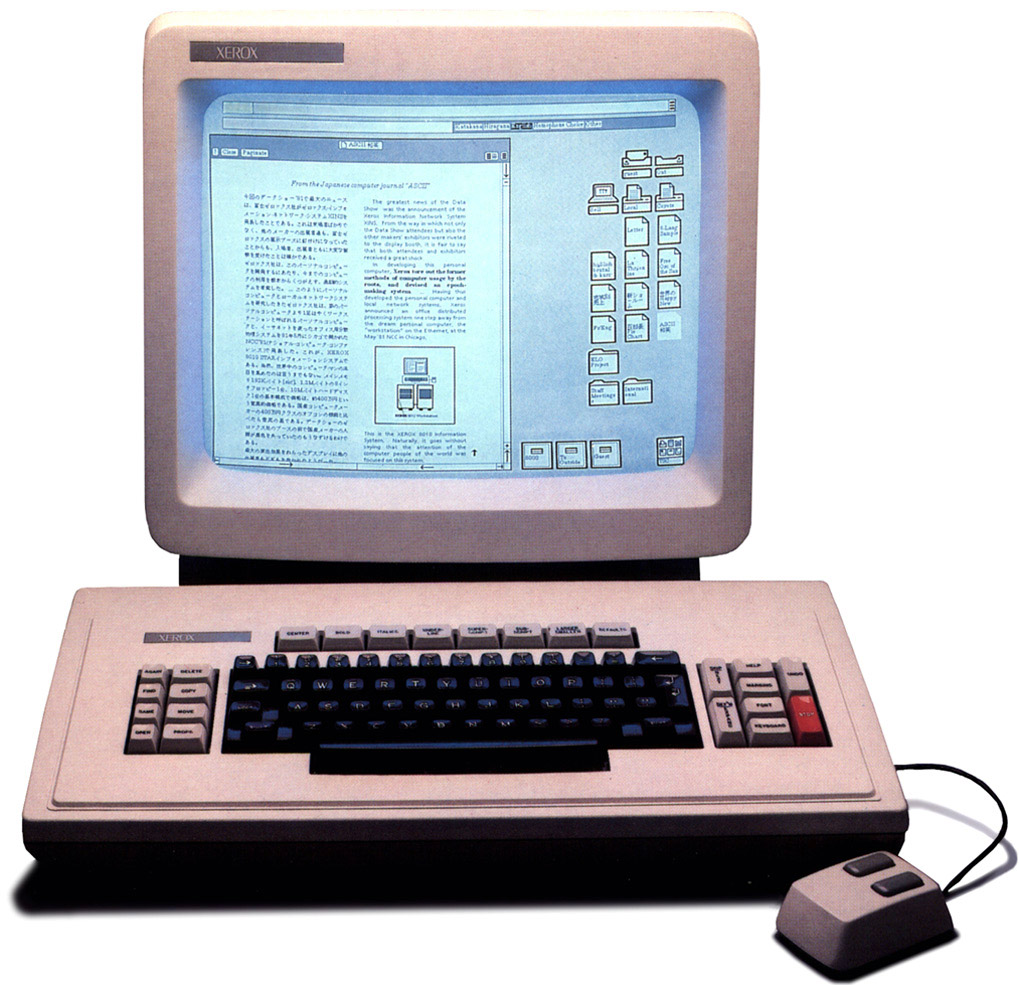
\includegraphics[scale=1]{../docs/lyaton/graphics/Xerox-Star.jpg}\\
\textbf{Xerox Star}\\
\begin{scriptsize}
Quelle: http://www.digibarn.com/collections/systems/xerox-8010/xerox-star-8010-large.jpg
\end{scriptsize}
\end{center}

\begin{center}
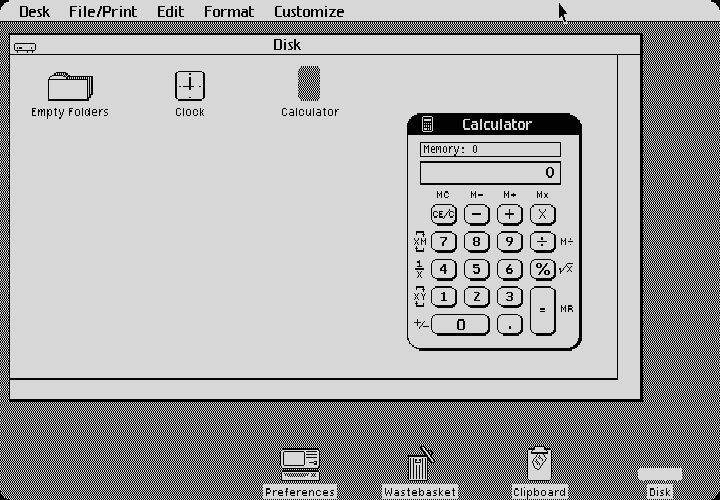
\includegraphics[scale=0.6]{../docs/lyaton/graphics/Apple-Lisa.png}\\
\textbf{Apple Lisa - Oberfläche (Nachgestellt)}\\
\begin{scriptsize}
Quelle: http://de.wikipedia.org/wiki/Apple\_Lisa\#/media/File:AppleLisa.png
\end{scriptsize}
\end{center}

\begin{center}
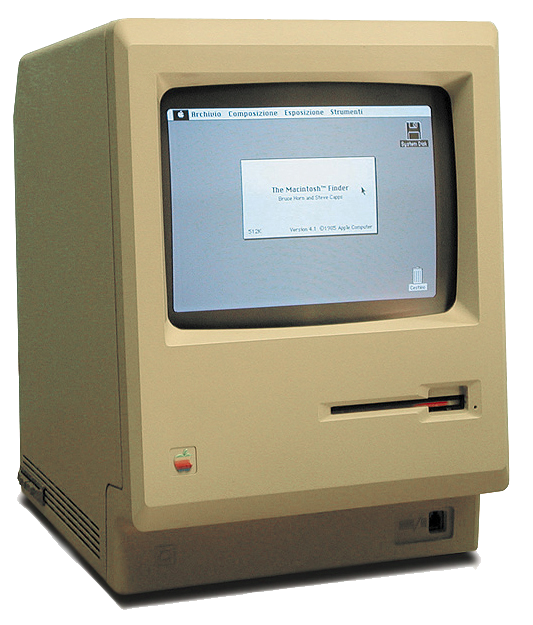
\includegraphics[scale=0.6]{../docs/lyaton/graphics/Apple-Macintosh.png}\\
\textbf{Apple Macintosh}\\
\begin{scriptsize}
Quelle: http://de.wikipedia.org/wiki/Grafische\_Benutzeroberfläche\#/media/File:Macintosh\_128k\_transparency.png
\end{scriptsize}
\end{center}

\begin{center}
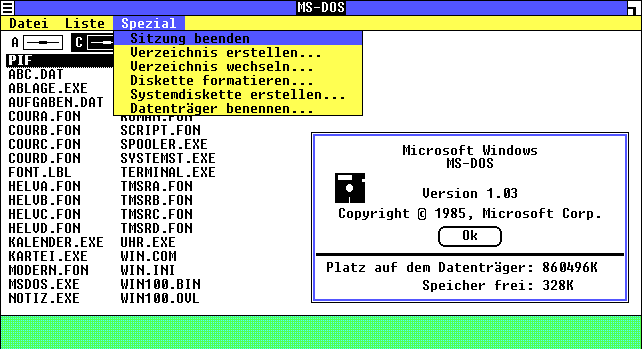
\includegraphics[scale=0.6]{../docs/lyaton/graphics/Windows-1_03.png}\\
\textbf{Windows 1.03}\\
\begin{scriptsize}
Quelle: http://de.wikipedia.org/wiki/Microsoft\_Windows\_1.0\#/media/File:Win1.03.png
\end{scriptsize}
\end{center}

\begin{center}
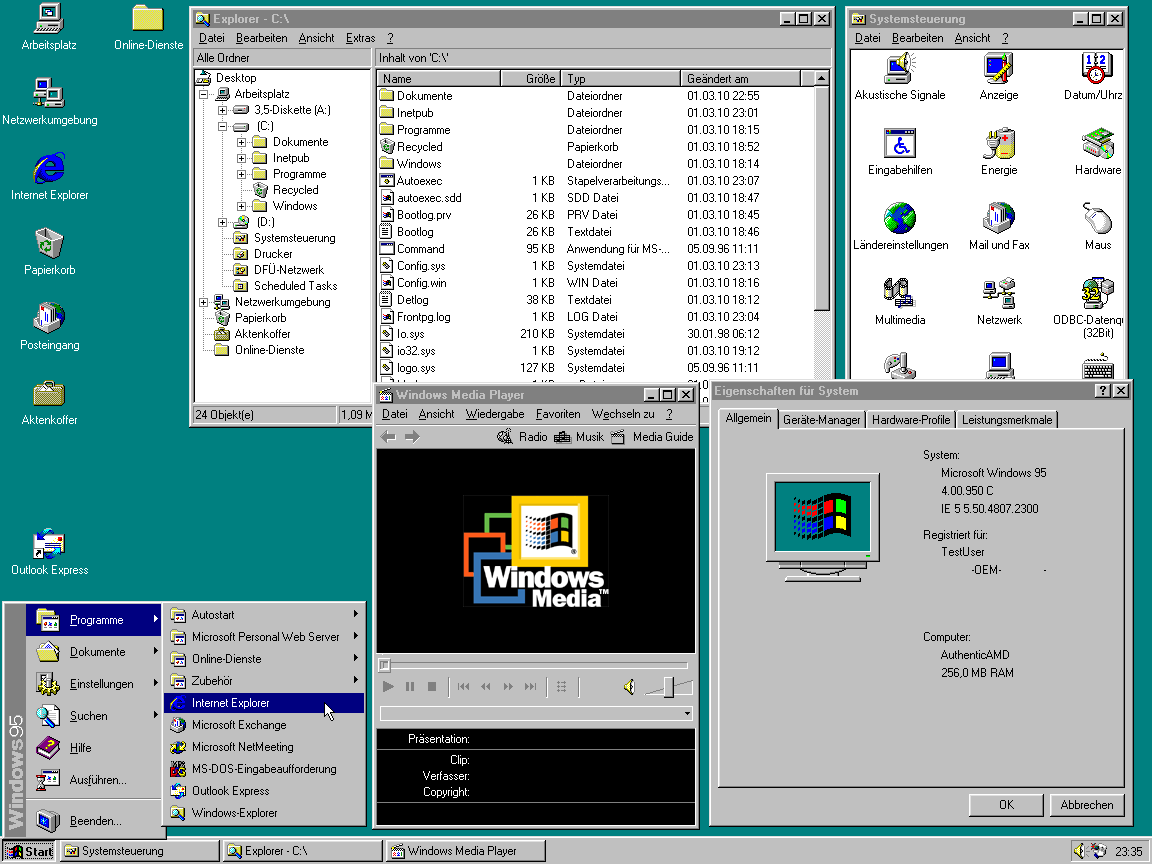
\includegraphics[scale=0.3]{../docs/lyaton/graphics/Windows-95.png}\\
\textbf{Windows 95}\\
\begin{scriptsize}
Quelle: http://de.wikipedia.org/w/index.php?title=Datei:Windows\_95\_C\_Startmenü\_System\_mit\_allen\_Updates\_2010-03-01.png
\end{scriptsize}
\end{center}

\begin{center}
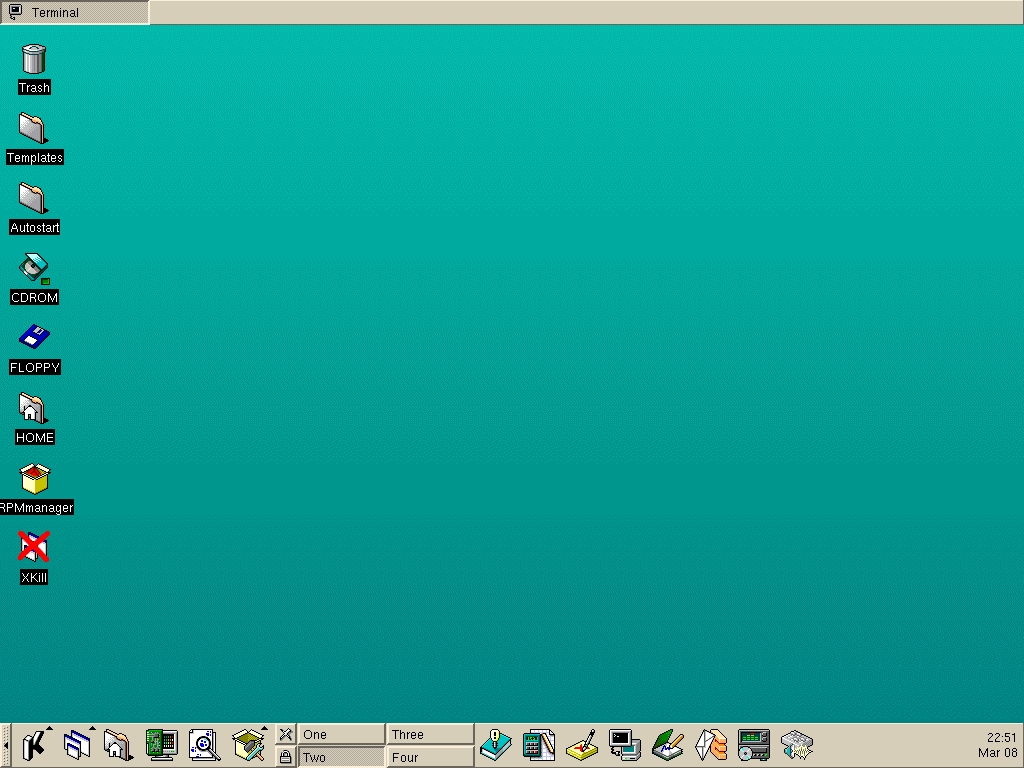
\includegraphics[scale=0.3]{../docs/lyaton/graphics/KDE_1_0.jpg}\\
\textbf{KDE 1.0}\\
\begin{scriptsize}
Quelle: http://de.wikipedia.org/wiki/Datei:KDE\_1.0.jpg\#/media/File:KDE\_1.0.jpg
\end{scriptsize}
\end{center}

\begin{center}
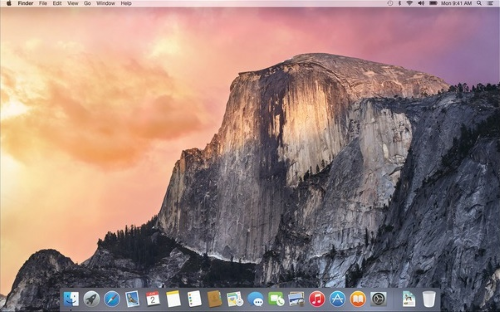
\includegraphics[scale=1]{../docs/lyaton/graphics/Apple_OS_X_Yosemite.png}\\
\textbf{OS X Yosmite}\\
\begin{scriptsize}
Quelle: http://en.wikipedia.org/wiki/OS\_X\_Yosemite\#/media/File:OS\_X\_Yosemite\_Desktop.png
\end{scriptsize}
\end{center}

\begin{center}
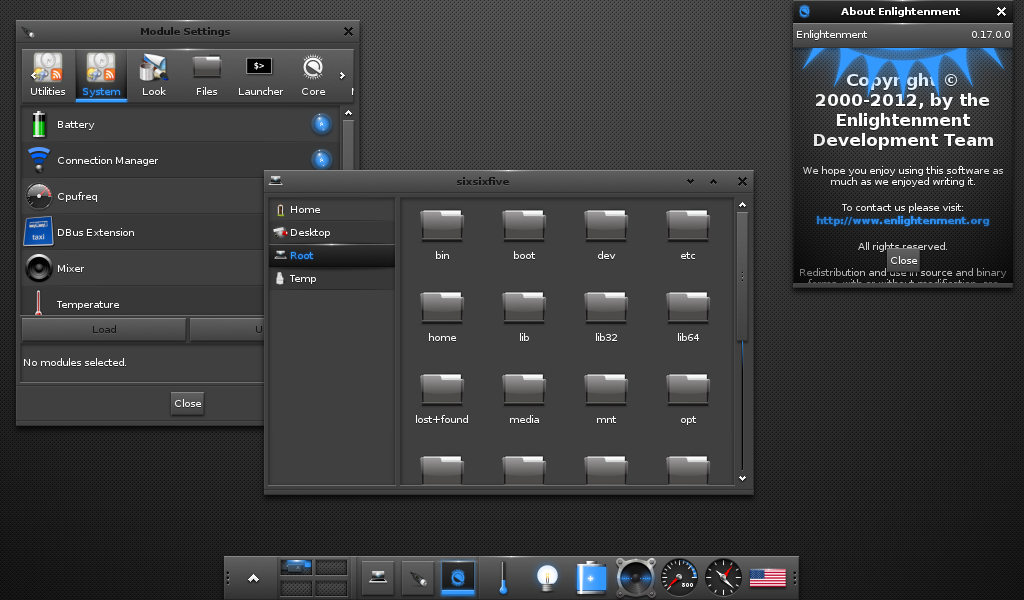
\includegraphics[scale=0.4]{../docs/lyaton/graphics/Enlightenment1700.png}\\
\textbf{Enlightenment 0.17}\\
\begin{scriptsize}
Quelle: http://de.wikipedia.org/wiki/Datei:Enlightenment1700.png\#/media/File:Enlightenment1700.png
\end{scriptsize}
\end{center}

\begin{center}
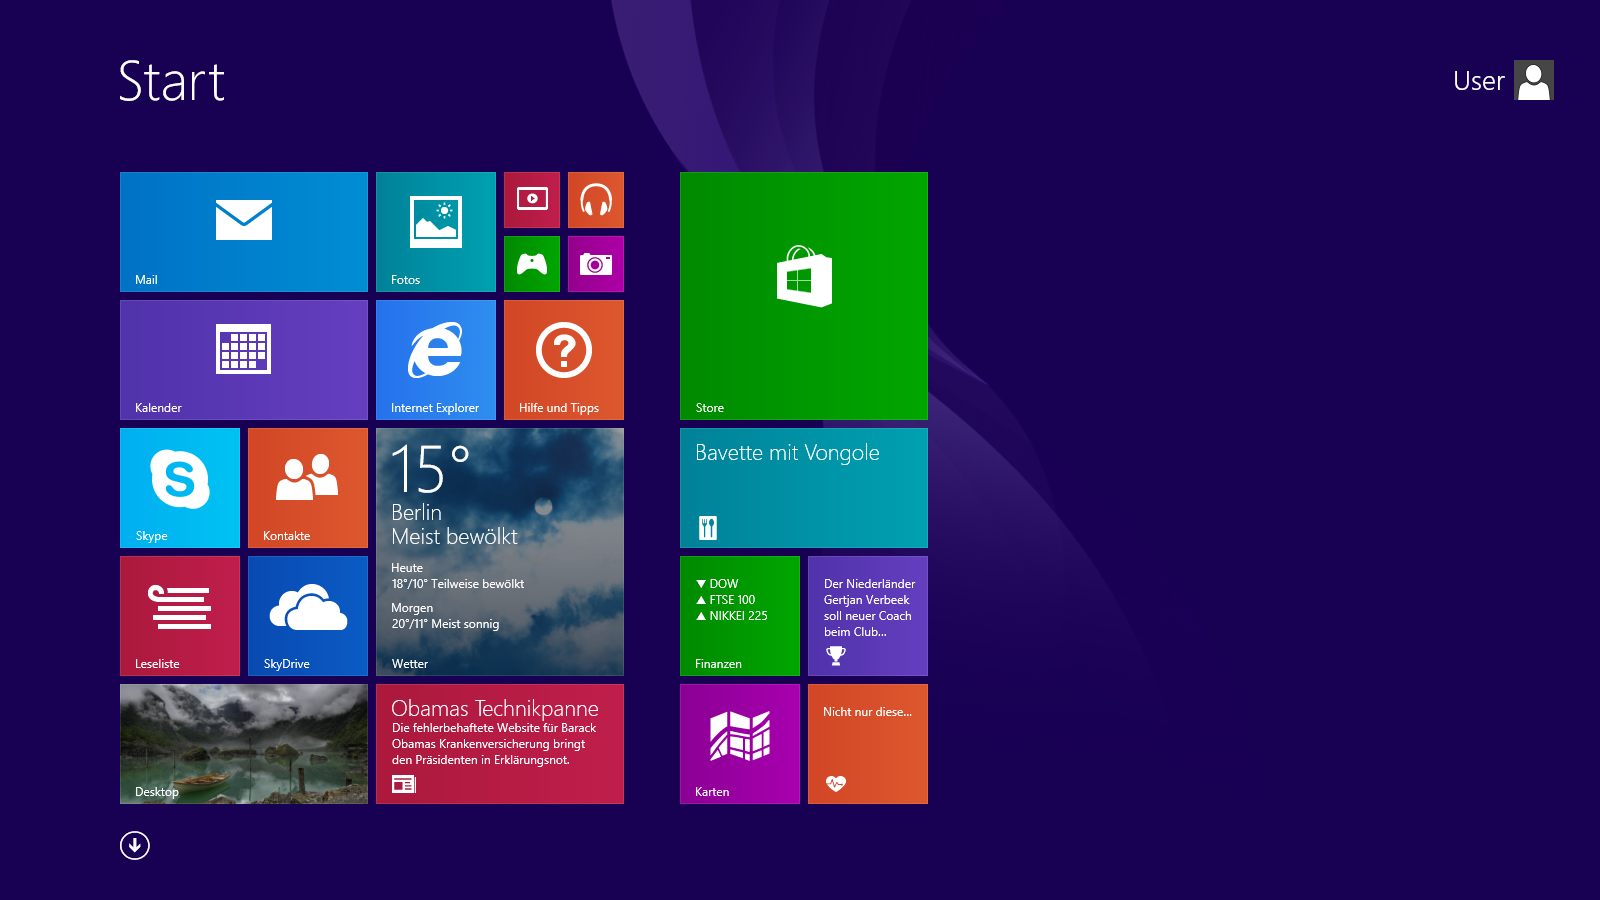
\includegraphics[scale=0.35]{../docs/lyaton/graphics/Windows_8_1.png}\\
\textbf{Windows 8.1}\\
\begin{scriptsize}
Quelle: http://de.wikipedia.org/w/index.php?title=Datei:Windows\_8.1\_ModernUI\_de\_germany.png
\end{scriptsize}
\end{center}

\subsection{Technischer Hintergrund}
\begin{flushright}
\begin{tiny}
Quellen: [305]
\end{tiny}
\end{flushright}
Die Benutzeroberfläche ist die Schnittstelle zum System. Mit dieser kann der Benutzer interagieren
\begin{center}
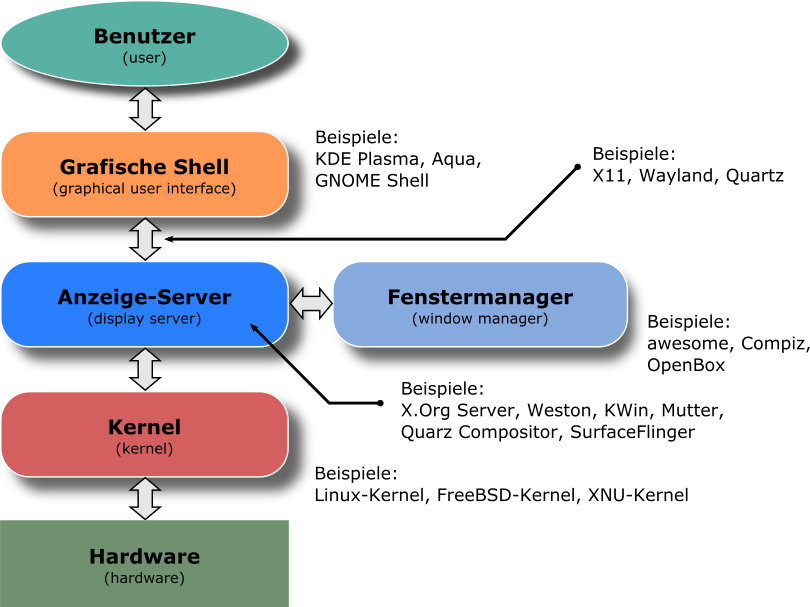
\includegraphics[scale=0.7]{../docs/lyaton/graphics/Graph.png}\\
\textbf{Schichten - Graphische Oberfläche}\\
\begin{scriptsize}
Quelle: http://de.wikipedia.org/wiki/Grafische\_Benutzeroberfläche\#/media/File:Schema\_der\_Schichten\_der\_grafischen\_Benutzeroberfläche.svg
\end{scriptsize}
\end{center}
In der obigen Abbildung wird ein üblicher Aufbau von Linux Systemen dargestellt.\\
Die einzelnen Schichten werden im Folgenden genauer erläutert: \\
\begin{itemize}
\item \textbf{Hardware}\\
Die Hardware kann durchaus varieren. Es gibt unzählige Hersteller für Grafikkarten. Auch die Hersteller von Prozessoren haben bereits Grafikkarten integriert (Onboard Grafikkarten). 
\item \textbf{Kernel}\\
Als Kernel wird das System bezeichnet, auf dem alles aufbaut.(z.B. Linux Kernel)
\item \textbf{Anzeige Server}\\
Der Anzeige Server stellt die Graphische Oberfläche zur Verfügung.(z.B. X.Org)
\item \textbf{Grafische Shell}\\
Die Grafische Shell kommuniziert mit dem Anzeige Server und teilt diesem mit was er darstellen soll. (z.B. KDE, Gnome) 
\item \textbf{Benutzer}\\
Zuletzt kommt der Benutzer, welcher durch die dargestellte Oberfläche mit Komfort seinen Rechner bedienen kann. 
\end{itemize}
\subsection{Normen}
\begin{flushright}
\begin{tiny}
Quellen: [306]
\end{tiny}
\end{flushright}
Die europäische Norm ISO 9241-110 beschreibt welche Aspekte ein graphische Benutzeroberfläche abdecken muss. (vgl. http://de.wikipedia.org/wiki/Grafische\_Benutzeroberfläche\#Technik)\\
Folgende Punkte werden in dieser Norm behandelt:
\begin{itemize}
\item Aufgabenangemessenheit\\
Damit wird beschrieben wie gut sich das Produkt für den Einsatz eignet. 
\item Selbstbeschreibungsfähigkeit\\
Die Selbstbeschreibungsfähigkeit sagt über die Orientierbarkeit am Produkt selbst aus. 
\item Steuerbarkeit\\
Diese beschreibt, wie gut das Produkt zu bedienen ist. 
\item Erwartungskonformität\\
Die Erwartungskonformität beschreibt die Beibehaltung einer durchgehenden Stiles.
\item Fehlertoleranz\\
Diese beschreibt, wie gut das Produkt mit eventuellen Fehlern umgehen kann.
\item Individualisierbarkeit\\
Die Individualisierbarkeit sagt aus, wie sehr ein Benutzer die Oberfläche anpassen kann. 
\item Lernförderlichkeit\\
Damit wird beschrieben, wie gut das Produkt dem Benutzer hilft, seine Qualifikationen zu erweitern. 
\end{itemize}
\chapter{Datenbank (Marko Stojanovi\'{c})}
\lfoot{Marko Stojanovi\'{c}}
\section{Allgemeines}
Datenbanksysteme sind für die Verwaltung von digitalen Daten zuständig. Heute stellen Datenbanksysteme einen zentralen Punkt im IT-Bereich dar. Zur heutigen Zeit haben sie auch eine wichtige Rolle in allen Unternehmen, da sämtliche Daten der Unternehmen auf diese Weise gespeichert werden. Dadurch ist ein Unternehmen auf die Verfügbarkeit, Vollständigkeit und Richtigkeit der Daten angewiesen. Deswegen ist sicherzustellen, dass die Datensicherheit gewährleistet ist, dies wird gesetzlich oder durch eine Behörde vorgeschrieben.\\

Zum Aufgabenbereich eines Datenbanksystems gehören speichern, lesen, löschen und ändern von Dateien. Dies muss für große Datenmengen effizient, widerspruchsfrei und dauerhaft gewährleistet sein. Auch geforderte Teilmengen müssen für Benutzer und Anwendungsprogramme, in verschiedensten Darstellungsformaten, bereitgestellt werden können.\\
\\Datenbanksysteme setzen sich grundsätzlich aus zwei Teilsystemen zusammen.
\begin{itemize}
\item Datenmanagementsystem (DBMS)\\
Dieses System ist für jegliche Organisationen im Datenbanksystem zuständig. Es gibt verschiedene Datenbankmanagementsystemmodelle.
\item Datenbank\\
Als Datenbank wird die Menge bzw. Sammlung von Daten bezeichnet.
\end{itemize} 
Datenbanken werden für alle Webseiten zur Datenverwaltung verwendet ( z.B.: Registrierungen, Einkäufe: ebay, amazon, ... ).
Microsoft Access und OpenOfficeBase eignen sich gut für kleinere Datenbanken (z.B.: kleinere Büros), weil die Handhabung durch die grafische Darstellung sehr leicht zu bedienen ist und den Mitarbeitern Schulungen erspart bleiben.
Diese eignen sich jedoch nicht als Datenbanken für Webdienste ( z.B.: Facebook, Twitter, ebay, ... ).\\

Häufig wird die Programmiersprache SQL (Structured Query Language), zur Kommunikation mit einer Datenbank, verwendet. Dabei ist bei der Erstellung von einer Datenbank zu beachten, dass keine Information mehrfach angegeben wird. Jede Information darf nur einmal vorkommen (bezogen auf die ID)! [421]

\section{Geschichte}
Bereits in den 1960er Jahren gab es Probleme beim Verarbeiten von Daten. Damals wurde eine Lösung entwickelt, bei der eine weitere Softwareschicht eingeschoben wurde. Diese lag zwischen der Dateiverwaltung (Betriebssystem) und den Anwendungsprogrammen. Dieser Lösungsversuch setzte sich jedoch nicht durch, da Datenspeicher in Form von Dateien individuell für einzelne Anwendungen erstellt wurden. Die Folge war, dass viel Zeit und Leistung zum Kopieren, Mischen und Restrukturieren der Dateien in Anspruch genommen werden musste.\\

1966 bis 1968 wurde IMS (Information Management System) von IBM, North American Rockwell und Caterpillar Tractors für das Apollo-Mondprogramm entwickelt, zur Verwaltung der Stücklisten, die verwalteten Datenbanken waren hierarchisch strukturiert. IMS gehört zu den ersten großen Datenbankmanagementsystemen (DBMS) mit der Sprache DL/I (Data Language One). IMS wurde vom Entwicklungsstart bis 1969 unter dem Namen  ICS (Information Control System) geführt. Heute wird IMS hauptsächlich in Bank- und Versicherungsunternehmen eingesetzt.\\

Zur gleichen Zeit wurde von CODASYL (COnference on DAta SYstems Languages) ein Netzwerk- Datenbanksystem entwickelt.\\

1970 wurde ein weiterer Fortschritt von Edgar Frank Codd erzielt. Im Rahmen einer Forschungsarbeit am IBM Almaden Research Center wurden die Grundlagen des ersten relationalen Datenbanksystems (System R) von Codd vorgestellt. Mit Open Source relationalem Datenbanksystem Ingres ( interactive graphics retrieval system) und der Abfragesprache QUEL folgte die Berkeley Groupe.\\

Oracle (damals SDL und RSI) nutzte Ergebnisse von System R und brachte SQL den Erfolgt.  Von IBM folgte SQL/DS und DB2.\\

Trotz einiger Kritikpunkte wurden in den 1980er Jahren hierarchische und netzwerkartige Systeme von vielen Behörden, Konzernen, Instituten und auch kleineren Unternehmen durch das relationale Modell ersetzt. Bis zu den 2000er Jahren, als Open-Source-Datenbankmanagementsysteme an Bedeutung erlangen, gab es keine großen Veränderungen. Die größten Marktanteile wurden von MySQL und PostgreSQL erzielt.
Als Reaktion von führenden Herstellern wurden gratis Versionen ihrer Produkte angeboten.\\

Seit 2001 wurde  NoSQL bekannter und gewann ebenfalls an Bedeutung, da es sich mit einem nicht-relationalen Konzept durchsetzten konnte. \\

Seit 2000 wird auch NewSQL oft verwendet. Es handelt sich um eine Klasse von modernen relationalen Datenbanken, welche die gleiche Skalierbarkeit wie NoSQL Systeme für Online-Transaktionen anbieten, und dabei immer noch auf SQL basieren. [422]

\section{Definitionen}
\subsection{Datensatz}
\begin{itemize}
\item Entsprechung einer logischen Struktur
\item Tupel
\item Zeile in einer Tabelle
\end{itemize}
\subsection{Datenfeld}
\begin{itemize}
\item kleinste Einheit eines Datensatzes
\item Attribut
\item Spalte in einer Tabelle
\end{itemize}
\subsection{Relation}
Tabelle (in RDMS)
\subsection{Schlüssel}
\begin{itemize}
\item dient zur eindeutigen Identifikation von Datensätzen
\item es gibt verschiedene Arten
\end{itemize}
\subsubsection{primary Key (Primärschlüssel)}
\begin{itemize}
\item wird zur eindeutigen Identifikation eines Datensatzes in relationalen Datenbanken eingesetzt
\item ist in allen Tabellen, in einer normalisierten Datenbank, enthalten
\item ist einmalig/eindeutig
\item oft verwendet als Datenbank- Index
\begin{itemize}
\item eindeutiger Primärschlüssel
\begin{itemize}
\item ein eindeutiger Schlüssel in einer Spalte
\item Datensätze werden durch einen eindeutigen Wert bestimmt
\item Beispiel: in einer  Mitarbeitertabelle kann die Sozialversicherungsnummer als primary Key verwendet werden
\end{itemize}
\item zusammengesetzter Primärschlüssel
\begin{itemize}
\item Kombination aus verschiedenen Attributen, da eindeutige Identifizierung nicht vorhanden
\item Kombinationen dürfen nur einmal vorkommen
\item Beispiel für zusammengesetzten Primärschlüssel: Vorname + Nachname + Geburtsdatum
\end{itemize}
\item Künstlicher Primärschlüssel
\begin{itemize}
\item keine eindeutigen Spalten oder Kombinationen aus Spalten
\item wird als zusätzliche Spalte in die Tabelle implementiert
\item auch Surrogate Key genannt
\item Praxis: Integer zur Datensatzidentifizierung
\end{itemize}
\end{itemize}
\end{itemize}
\subsubsection{Sekundärschlüssel}
\begin{itemize}
\item Attributgruppen, welche einzelne oder mehrere Datensätze beschreiben
\item Beispiel: in Adresstabellen kann die Postleitzahl als Sekundärschlüssel definiert werden
\item nicht zwingend notwendig und nicht unbedingt einmalig vorkommend
\item hilfreich bei Suchanfragen
\end{itemize}
\subsubsection{Fremdschlüssel}
\begin{itemize}
\item Attribut oder Attributkombinationen einer Tabelle
\item zeigt auf den Primärschlüssel einer anderen oder der gleichen Tabelle
\end{itemize}
[423]
\section{Funktionen}
Zu den wichtigsten Funktionen von Datenbankmanagementsystemen zur heutigen Zeit gehören:
\begin{itemize}
\item Daten verändern, löschen, speichern
\item Metadatenverwaltung\\
Das sind Daten über Daten, z.B.: Größe einer Datei, Erstellungsdatum
\item Maßnahmen zur Datensicherheit, Datenintegrität und Datenschutz
\item Transaktionskonzept (Gewährleistung von Mehrbenutzerbetrieb)
\item Anfrageoptimierung/- anpassung
\item Verwendungsmöglichkeiten von: 
\begin{itemize}
\item Datenbanktrigger\\
Funktion von unterschiedlichen (relationalen) Datenbankmanagementsystemen, welche nach Manipulation von expliziten Daten aufgerufen wird und ein integriertes Programm startet, dieses kann die Manipulation verhindern, erlauben oder auch andere Aktionen ausführen
\item Stored Procedures (Gespeicherte Prozeduren)\\
mit einem Befehl ist ein Client in der Lage eine ganze Reihe von (gespeicherten) Anweisungen zu starten
\end{itemize}
\item Informationen des verwendeten Datenbankmanagementsystems
\begin{itemize}
\item Kennzahlen
\item Betrieb
\item Technik
\end{itemize}
\end{itemize}
[424]
\section{Datenbanksysteme}
Ein Datenbanksystem besteht immer aus einem DBMS und der dazugehörigen Datenbank. Ein Datenbanksystem muss gewährleisten, dass auf Festspeichern abgespeicherte Daten, auch nach einem unvorhergesehenen Ausfall des Systems (z.B.: Stromausfall), wieder ohne Veränderungen und Verluste aufgerufen werden.\\
Es bietet eine Schnittstelle zwischen dem DBMS und der Datenbankanwendung zur  Abfrage, Auswertung, Veränderung und Verwaltung der Daten an. [425]

\begin{center}
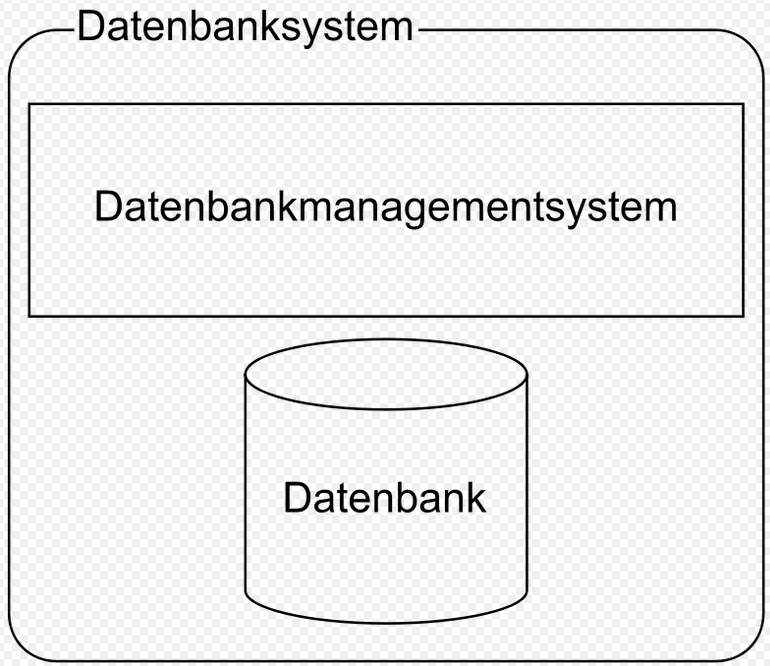
\includegraphics[scale=0.3]{img/dbs.png}\\
Datenbanksystem besteht aus: Datenbank und Datenbankmanagementsystem (Quelle: http://de.wikipedia.org/wiki/Datenbank\# Komponenten\_ eines\_ Datenbanksystems)
\end{center}

\subsection{Datenbank}
Theoretisch ist eine Datenbank ein zusammengehöriger Datenbestand. 
Diese Datenmenge wird auf einen Festspeicher abgelegt und für alle Anwendungen für den Benutzer von einem DBMS zur Verfügung gestellt.\\

Zu beachten ist, dass unter Datenbank oft das DBMS und die Daten gemeint werden, nicht die dazugehörige Datenbankanwendungssoftware. Diese besteht oft aus Computerprogrammen, welche über ein Datenbanksystem ihre notwendigen Daten speichern.
\\Beispiele: Auftragsverwaltung und Bestellwesen, Kunden- und Adressverwaltung, Rechnungserstellung. [425]

\subsection{Datenbankmanagementsysteme}
Das DBMS ist die Verwaltungssoftware, welche für die Organisation der strukturierten  Speicherung der Daten und zur Kontrolle der gesamten Lese, Lösch- und Schreibzugriffe auf die Datenbank zuständig ist.
Diese Software wird für das Datenbanksystem installiert und konfiguriert und durch diese Software wird auch das Datenbankmodell bestimmt.
Da die Funktonalität und die Geschwindigkeit von DBMS abhängen, ist die Auswahl gut zu durchdenken.
DBMS sind hochkomplexe Softwaresysteme.\\

RDBMS wird oft als Abkürzung verwendet, weil das relationale DBMS am meisten Verwendung findet. [425]

\section{Relationales Datenbankmanagementsystem}
Das relationale Datenbanksystem findet in der Praxis am häufigsten Verwendung.
Bei Relatinalen Datenbanksystemen können Felder aus verschiedenen Tabellen durch einen Primärschlüssel verbunden werden.\\

Relationale Datenbanken werden in Computersystemen zur elektronischen Datenverwaltung eingesetzt. Das dazugehörige relationale Datenbankmodell, wurde 1970 von Edgar F. Codd das erste Mal entworfen und ist tabellenbasiert. Dieses Modell findet heute auch häufigen Einsatz, obwohl es einige Mängel aufweist. Als Datenbankmanagementsystem, wird das sogenannte relationale Datenbankmanagementsystem (RDBMS, Relational Database Management System) verwendet. Die Datenbanksprache SQL (Structured Query Language) wird zur Manipulation und zum Aufruf der Daten eingesetzt.\\

Die Basis von relationalen Datenbanken ist die mathematische Definition einer Tabelle, die sogenannte Relation. Alle Aktivitäten auf Relationen werden von Relationen-Algebra festgelegt. Damit ist ersichtlich, dass die relationale Algebra die theoretische Basis von SQL ist. [426]

\subsection{Prinzip eines RDBMS}
Eine relationale Datenbank besteht aus vielen Tabellen (Relationen), in denen Datensätze gespeichert werden. Durch das Relationsschema werden Anzahl und Attributtypen der Relation bestimmt. Die Veranschaulichung einer Tabelle verläuft über die Attribute A1 bis An in den Spalten.\\

Die Funktion kann am Beispiel von einem Buch in einer Bücherei einfach gezeigt werden. Zur Beschreibung des Buchs in der Datenbank kann beispielsweise angegenben werden: Buch- ID, Autor, Titel, Aufnahmedatum, Verlag, Verlagsdatum, ...
\\Zur Beschreibung eines Datensatzes muss mindestens ein eindeutiger, unveränderlicher und einmal vorkommender Schlüssel vorhanden sein. Ein sinnvoller Primärschlüssel in diesem Beispiel ist Buch- ID. Der Schlüssel ist nicht für die Position des Datensatzes in der Tabelle zuständig, sondern für die eindeutige Identifikation. [426]

\begin{center}
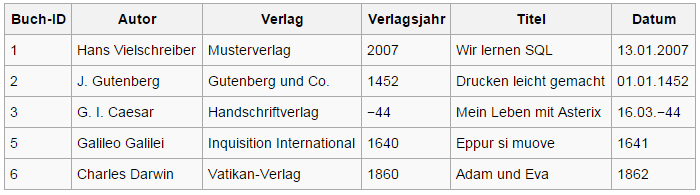
\includegraphics[scale=0.8]{img/relation_DB.png}\\
Beispiel einer Relation ("{}Buch"{})(Quelle: http://de.wikipedia.org/wiki/Relationale\_ Datenbank\# Grundlegende\_ Konzepte)
\end{center}

\subsection{Tabellen}
Die Nutzung von Verbindungen zwischen Tabellen wird zur Verfügung gestellt. Beispielsweise kann eine Datenbank in einer Bibliothek folgendermaßen erstellt werden.\\

Es werden drei Tabellen eingerichtet mit den Namen "{}Buch"{}, "{}Nutzer"{} und eine zusätzliche "{}Entliehen"{}.
\begin{itemize}
\item Tabelle "{}Buch"{}\\
Diese Tabelle enthält für jedes Buch einen eigenen Datensatz der sich aus den Attributen (Spalten) zusammensetzt.
\begin{itemize}
\item Attribute: Buch- ID, Autor, Titel, Verlag, ...
\item Primärschlüssel: Buch- ID
\end{itemize}
\item Tabelle "{}Nutzer"{}\\
Diese Tabelle enthält alle angemeldeten Büchereibenutzer.
\begin{itemize}
\item Attribute dieser Tabelle: Nutzer- ID, Vorname, Nachname, ...
\item Primärschlüssel: Nutzer- ID
\end{itemize}
\item Tabelle "{}Entliehen"{}\\
Diese Tabelle enthält Informationen über die Vergabe und die Verfügbarkeit von Büchern.
\begin{itemize}
\item Attribute dieser Tabellen sind: Buch- ID (Tabelle "{}Buch"{}), Nutzer- ID (Tabelle "{}Nutzer"{}), ...
\item Nutzer- ID werden in dieser Tabelle einer Buch- ID zugeordnet.
\item weitere Attribute könnten sein: Ausleihdatum, Rückgabedatum, ...
\end{itemize}
\end{itemize}

\begin{center}
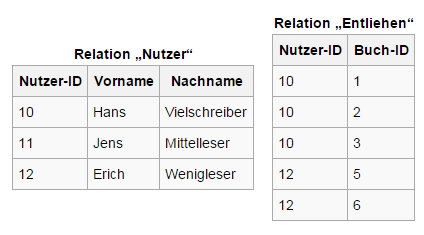
\includegraphics[scale=0.8]{img/tabellen.png}\\
Beziehungen zwischen Tabellen (Quelle: http://de.wikipedia.org/wiki/Relationale\_ Datenbank\# Beziehungen\_ zwischen\_ Tabellen)
\end{center}
[426]
\subsection{Datenbankschema und Modellierung}
Das Schema in relationalen Datenbanken ist entscheidend für die Speicherung der Daten und deren Beziehung zueinander. Die Erstellung eines Datenbankschemas wird als Datenmodellierung bezeichnet.\\

Das sogenannte "{}Entity- Relationship- Modell"{} wird zur Erstellung von Datenschemas oft eingesetzt. Auf diese Weise wird ein konzeptuelles Schema entwickelt, dass von einem Datenbankmanagementsystem implementierbar ist. Dieser Vorgang wird Entwurf oder Datenmodellabbildung genannt.\\

Um Redundanzen zu reduzieren und Anomalien zu verhindern ist ein entscheidender Vorgang bei Modellierungsprozessen erforderlich, die sogenannte "{}Normalisierung"{}. Die Wartung der Datenbanken wird unkomplizierter und die Konsistenz (Korrektheit der gespeicherten Daten) der Daten wird garantiert.\\

Edgar F. Codd erstellte vier Normalformen, welche heute noch bei relationalen Datenbankentwürfen eingesetzt werden und noch durch zusätzliche erweitert werden. 
[427]
\subsection{Alternative Datenbankmodelle}
Es sind noch viele weitere Datenbankmanagementsystem vorzufinden, welche durch Kombinationen aus den folgenden Systemen entstanden sind (objektrelationales Modell).
%http://de.wikipedia.org/wiki/Datenbank#Datenbankmodell
\subsubsection{Objektorientiertes Datenbankmodell}
Objektdatenbanken oder Objektorientierte Datenbanken basieren auf dem Objektdatenbankmodell. Hier werden Daten als Objekte verwaltet, als Anlehnung an die Objektorientierung. Das Objektdatenbanksystem besteht aus dem dazupassenden Datenbankmanagementsystem, welches als Objektdatenbankmanagementsystem bezeichnet wird und der Objektdatenbank.\\

Objekt steht normalerweise für einen Begriff aus der realen Welt und beinhaltet auch die dazugehörigen Attribute, welche das Objekt genau beschreiben (z. B.: Objekt: Auto; dazugehörige Eigenschaften: Farbe, Gewicht, ...). Das Ablegen von Daten und Methoden erfolgt gemeinsam in einem Objekt.\\

Das Objektdatenbankmanagementsystem hat, neben den grundsätzlichen Anforderungen, zusätzliche zu erfüllen:
\begin{itemize}
\item Da sich ein Objekt aus beliebig vielen verschiedenen Datentypen ergibt ist die Verwaltung komplexer Objekte zu gewährleisten
\item Allen Objekten wird eine einmalige Identifikation OID zugeordnet, zur Sicherstellung der einzelnen Objektidentitäten
\item Da Zugriffe mittels Methoden ermöglicht werden, ist die Kapselung der Objekte (Konzept der objektorientierten Programmierung) einzuhalten
\item Objekte werden Objektklassen zugeteilt.
\item Klassenhierarchien dienen zur Anordnung von Objektklassen.
\item Bei vererbten Objekten werden überladene Methoden benutzt, dies kommt durch späte Bindungen zustande.
\item Eine Turning-vollständige Manipulationssprache (DML) muss vom Objektdatenbankmanagementsystem zur Verfügung gestellt werden.
\item Es gibt weitere variable Eigenschaften, welche zusätzlich von den verschiedenen Objektdatenbankmanagementsystem angeboten werden.
\end{itemize}
Von ODMG wurde die Abfragesprache OQL (Object Query Language)und als Datenmanipulationssprache ODL (Object Definition Language) festgelegt. [428]

\subsubsection{Dokumentenorientiertes Datenbankmodell}
Bei dieser Art von Datenbank werden Dokumente als Basis zur Datenspeicherung verwendet. Lotus Notes ist die am häufigsten benutze dokumntenorientierte Datenbank.\\

Eine dokumentenorientierte Datenbank besteht aus einzelnen Dokumenten, während beispielsweise die relationale Datenbank aus genauen Datenbankschemas zur Organisation der Relationen besteht. Bei den Dokumenten kann es sich um strukturierte Dateien mit Standard- Dateiformaten handeln (z. B.: Dateien von Programmen zur Textverarbeitung) oder auch um Binary Large Objects.\\

Binary Large Objects sind aus Sicht des Datenbankzugriffs nicht weitgehend strukturiert (z. B.: Videofilme im mped- Format). Weitere Datenformate können sein:
\begin{itemize}
\item JSON- Objekte
\item YAML- Dokumente
\item XML- Dokumente
\item usw.
\end{itemize}
Alle Dokumente werden für einen einmaligen und eindeutigen Identifikator gekennzeichnet.\\
\\Beispiele für andere dokumentenorientierte Datenbankmanagementsystem:
\begin{itemize}
\item Basex
\item CouchDB
\item eXist
\item MongoDB
\item RavenDB
\item MarkLogic Server
\end{itemize}
[429]
\subsubsection{Netzwerkdatenbankmodell}
Die Veröffentlichung des Netzwerk- Datenbankmodells erfolgte ca. zur gleichen Zeit wie die des relationale Datenbankmodells.\\
\\Eigenschaften eines Netzwerkdatenbankmodells:
\begin{itemize}
\item keine strenge Hierarchie
\item Datenfelder bestehen aus einem Namen und einem Wert
\item m:n Beziehungen sind möglich (Datensätze können mehrere Vorgänger besitzen)
\item mehrere Datensätze können an erster Stelle stehen
\end{itemize}
Der große Vorteil bei diesem Modell ist, dass verschiedene Suchwege zur Verfügung stehen. Dies kann, aber auch zum Nachteil werden und wenn vom Programmierer ein bestimmter Lösungsweg vorgesehen ist. Die Übersichtlichkeit wird schlechter mit der zunehmenden Größe des Modells immer geringer.\\

Das Netzwerkdatenbankmodell gilt heute als Verallgemeinerung des hierarchischen Datenbankmodells. [430]

\subsubsection{Hierarchisches Datenbankmodell}
Das hierarchische Datenbankmodell ist das älteste Datenbankmodell das es gibt. Die Darstellung erfolgt in Form einer hierarchischen Baumstruktur. Früher wuden das Modell von vielen Betriebssystemen für Dateisysteme verwendet, zur Abbildung der Daten. Zur heutigen Zeit ist das Modell in wenigen Anwendungen noch vorzufinden.\\
\\Eigenschaften
\begin{itemize}
\item Alle Datensätze haben nur einen Vorgänger.
\item Der Datensatz, durch den die Wurzel der Baustruktur erstellt wird, ist die einzige Ausnahme
\item Verknüpfungen werden in der Baustruktur dargestellt und durch Eltern- Kinder- Beziehungen ermöglicht.
\item Das verknüpfen zweier Baumstrukturen ist nicht realisierbar.
\item Das Modell ist starr und bietet geringe Freiheiten für den Programmierer.
\end{itemize}
Das hierarchische Datenbankmodell konnte in den letzten Jahren wieder einen Erfolg feiern, weil es im Bereich der XML- Entwicklung effizient genutzt wird. [431]

\subsection{Sicherheit}
Bei einem relationalen Datenbankmanagementsystem werden relatioanle Daten auf einem Speichermedium abglegt. Es werden zu den eigentlichen Daten auch Informationen über das Datenschema und Berechtigungen gespeichert. Durch das Abspeichern der Berechtigungen wird Datensicherheit (Schutz gegen Datenverlust und verbotet Zugriffe) gewährleistet. Metadaten werden als "{}data dictionary"{} bei Datenbankmanagementsystemen bezeichnet.\\

Das Sichern des Datenbankinhaltes durch Backups ist ebenfalls zu gewähleisten. Probleme bei der Performance sind in Praxis bei diesen Vorgängen zu beobachten, da die Manipulation von Daten beschränkt wird.\\
%http://de.wikipedia.org/wiki/Datenbank#Datensicherheit

Das Transaktionskonzept gehört auch zu den wichtigsten Aspekten der Datensicherheit. Dieses soll sogenannte "{}Race Conditions"{} verhindern, welche beim nicht autorisierten parallelen Aufruf von Dateien aus der Datenbank entstehen können. Daten könnten gleichzeitig von mehreren Benutzern verändert werden, diese würde zu inkonsisten Daten führen und Änderung würden vom Zufallen abhängig sein. Das Lösung ist es nur einem Benutzer die Berechtigung zu erteilen Änderungen an den Daten vornehmen zu können, währen andere gesperrt bleiben.\\
%http://de.wikipedia.org/wiki/Datenbank#Transaktionen

Das Sicherstellen der Integrität erfolgt durch "{}Constraints"{}. Es handelt sich um Regeln im Managementsystem, die zur Beschreibung der Datenveränderungen dienen. Foreign Key Constraint ist der wichtigste bei relationalen Datenbanksystemen. Durch diesen werden Daten, die von anderen Tabellen benötigt werden nicht gelöscht. Andere Bedingungen regeln das Duplizieren, einzelne Inhalte bestimmter Datenfelder, ...
%http://de.wikipedia.org/wiki/Datenbank#Datenintegrit.C3.A4t
[432]
\subsection{Gleichzeitige Zugriffe}
Um ausgewählte Operationen ausführen zu können, werden beim Zugriff auf die Daten Berechtigungen geführt, damit beim "{}gleichzeitigen"{} Zugriff verschiedener Programme bzw. Benutzer vom Datenbankmanagementsystem entschieden werden kann, welcher Zugriff als erster erfolgen darf.\\
Bei diesem Prozess wird folgendes Verwaltet:
\begin{itemize}
\item locks (Sperren)
\item Systemprotokolle
\item transaktionsorientiertes arbeiten des DBS
\end{itemize}
Durch diese Fähigkeiten wird ein Datenbanksystem im Allgemeinen definiert. Es gibt Dateisysteme mit wesentlichen Erweiterungen.\\

Alle Fehler, die aufgrund von gleichzeitigen Zugriffen auf die Datenbank erfolgen, werden als Anomalien im Mehrbenutzerbetrieb bezeichnet. [433]
%http://de.wikipedia.org/wiki/Datenbank#Mehrbenutzerf.C3.A4higkeit

\section{Sprachen}
Von einem Datenbanksystem wird eine Datenbanksprache zur Kommunikation zur Verfügung gestellt. Diese Schnittstelle muss folgendes erfüllen:
\begin{itemize}
\item Datenabfrage und Manipulation (DML)
\item Verwaltung der Datenbank und Datenstrukturen- Definitionen (DDL)
\item Steuerung der Berechtigungen (DCL)
\end{itemize}
Von der Datenbanksprache abhängig sind diese Kategorien voneinander getrennt oder in einer Sprache zusammengefasst, wie beim relationalen Datenbankmanagementsystem (SQL). Es gibt auch verwaltungsgetrennte Sprachen welche nicht alle Kategorien enthalten. [434]
\section{SQLite}
Bei SQLite handelt es sich um ein relationales Datenbankmanagementsystem, welches in einer, in C programmierten, Bibliothek enthalten ist. Es handelt sich nicht wie bei vielen anderen DBMS um eine client- Server Datenbankmodell. Es wird nämlich nur in ein Programm eingebunden.\\

SQLite ist eine oft verwendete Möglichkeit, wenn eine eingebundene Datenbanksoftware für lokale Speicherungen in ein Programm gefordert wird (z. B.: Webserver). SQLite findet sich heute in einem breiten Spektrum von Einsatzgebieten (weitverbreitete Browser, Betriebssysteme, Embedded Systems, ...).\\
Dadurch hat SQLite eine Anbindung an viel Programmiersprachen. [435]

\subsection{Geschichte}
SQLite wurde von D. Richard Hipp 2000 entwickelt, während er für den US- amerikanischen Rüstungskonzern General Dynamics arbeitete. Er entwickelte Software zur Steuerung von Lenkwaffenzerstörern, welche ursprünglich HP- UX basierten mit einer IBM Informatik Datenbank ausgestattet war. Das damahlige Entwicklungsziel war es, ein Programm ausführen zu können ohne eine Installation eines dazugehörigen Datenbankmanagementsystems oder die Bestätigung eines Datenbankadministrators.\\

Die Basis der Syntax und Semantik holte sich Hipp aus der PstgreSQL 6.5 Dokumentation. Im August 2000 wurde SQLite Version 1.0 vorgestellt. Die Speicherung wurde damals auf der Basis von gdbm realisiert (GNU Database Manager). SQLite 2.0 ersetzte gdbm mit einer B-tree Implementierung, durch welche Transaktionen ermöglicht waren. SQLite 3.0 wurde zum Teil von America Online entwickelt weiter ergänzt. \\

2011 gab Hipp bekannt, dass er eine UnQL- Schnittstelle Implementieren möchte und UnQL weiter entwickeln möchte. UnQL ist eine eingebundene dokumentenorientierte Datenbank. [436]

\subsection{Eigenschaften}
SQLite hat viel wichtige Eigenschaften, zu den wichtigsten Eigenschaften zählen:
\begin{itemize}
\item (Atomarität, Konsistenz, Isolation und Dauerhaftigkeit (ACID) von Transaktionen, selbst im Fall eines Systemabsturzes oder eines Stromausfalles
\item keine Installation oder weitere Verwaltungen oder Konfigurationen nötig
\item komplette SQL- Implementierung mit Erweiterungen: Teilindizes, allgemeine Tabellenausdrücke, ...
\item gesamte Datenbank ist in eine Datei gespeichert ("{}single disk file"{}), optial für den Einsatz in Anwendungen
\item Terabyte- Datenbanken und Gigabyte große strings und blobs werden unterstützt.
\item kleine Code- Bilanzen, welche kleiner als 500 KB, sind vollständig konfigurierbar
\item einfache API (Schnittstelle)
\item gut kommentierter Quellcode
\item erhältlich als ein ANSI-C Quellcodedatei, welche einfach kompiliert werden kann und deswegen leicht in größere Projekte eingebunden werden kann
\item Plattformübergreifend: Android, * BSD, iOS, Linux, Mac, Solaris, VxWorks und Windows (Win32, WinCE, WinRT)\\
einfache Portierung auf andere Systeme
\item Quellen sind in der sogenannten "{}Public Domain"{}, diese erlaubt die Benutzung sämliche Zwecke
\item usw.
\end{itemize}
[437]
\subsection{Syntax}
Die Syntax von SQLite ist der Syntax von SQL weitgehend identisch. Die Unterscheidung liegen darin, dass einige Fähigkeiten von SQL nicht unterstützt werden und dafür eigene eingebaut sind. Die Syntax wird mithilfe von Syntaxdiagrammen erklärt.
Diese sind sehr einfach zu lesen und im Prinzip selbsterklärend. Es werden Argumente in der richtigen Reihenfolge aufgelistet und auch die verschiedenen dazugehörigen Optionen. Es gibt zur jeder möglichen Funktion ein entsprechendes Syntaxdiagramm. Die wichtigsten und grundlegendsten Diagramme, welche zur Realisierung der Datenbank nötig waren, werden im Folgenden aufgelistet. [438]

\begin{center}
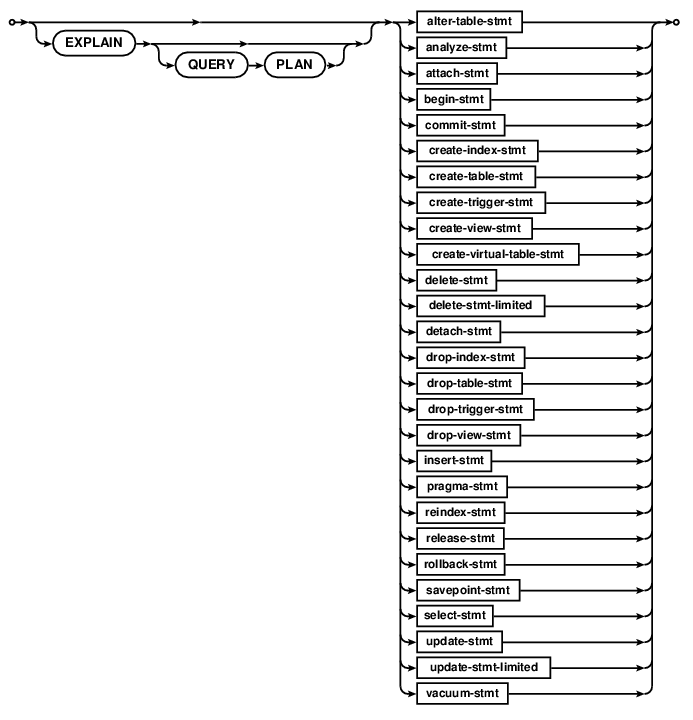
\includegraphics[scale=0.8]{img/sqlite_syntax.png}\\
allgemeine SQLite Syntax (Quelle: http://www.sqlite.org/syntax/sql-stmt.html)
\end{center}

\begin{center}
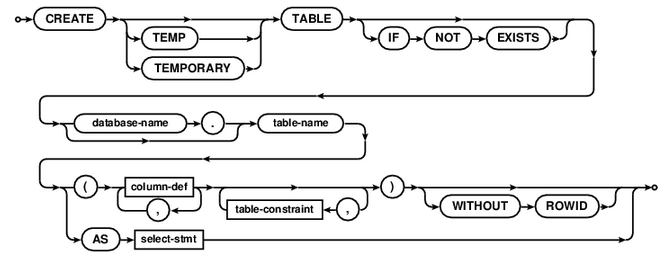
\includegraphics[scale=0.8]{img/sqlite_create.png}\\
erstellen einer Tabelle (Quelle: http://www.sqlite.org/lang\_ createtable.html)
\end{center}

\begin{center}
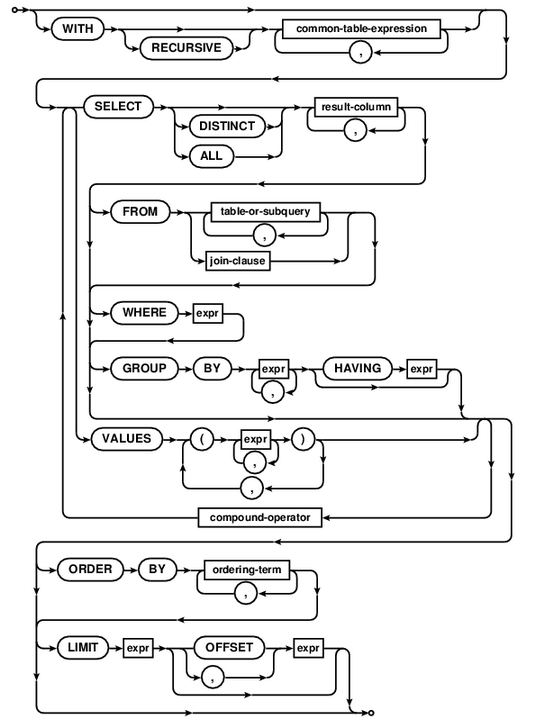
\includegraphics[scale=0.8]{img/sqlite_select.png}\\
Argumente beim Auswählen von Daten (Quelle: http://www.sqlite.org/lang\_ select.html)
\end{center}

\begin{center}
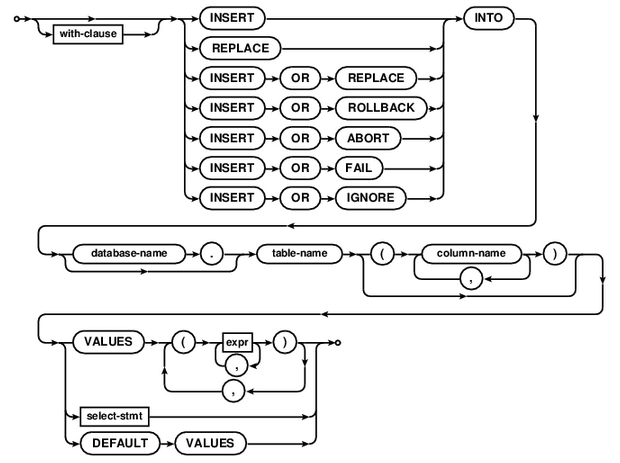
\includegraphics[scale=0.8]{img/sqlite_insert.png}\\
Daten in einer Tabelle speichern (Quelle: http://www.sqlite.org/lang\_ insert.html)
\end{center}

\subsection{Vor- und Nachteile}
Bei Verwendung von SQLite entscheidet der Einsatzbereich ob es sich bei einer Eigenschaft um einen Vor- oder Nachteil handelt. Grundsätzlich werden Eigenschaften von SQLite folgender Maßen gesehen.
\subsubsection{Vorteile}
\begin{itemize}
\item keine Installationen erforderlich
\item Unterstützung von SQL- Syntax
\item sehr klein (kleiner Speicherplatzverbrauch für das System)
\item hohe Geschwindigkeit
\end{itemize}
\subsubsection{Nachteile}
\begin{itemize}
\item Speicherung der Datenbankdatei auf dem Webserver, keine zusätzliche Anwendung nötig
\item keine echten gleichzeitigen Datenbankzugriffe möglich, nur darauf folgende
\item keine Integrität der Daten
\end{itemize}
[439]

\chapter{Kryptologie (Alin Porcic)}\label{chap:krypto}
\lfoot{Alin Porcic}
\section{Allgemeines}

Die Kryptologie befasst sich mit der Informationssicherheit und hat in der heutigen modernen Zeit einen sehr wichtigen Stellenwert eingenommen. Unzählige Informationen werden weltweit ausgetauscht und dabei kommt es öfter vor, dass die zu übertragenen Informationen einen hohen Wert haben können. Der Wert dieser Informationen geht dann verloren, wenn ein Unbefugter die Aussage der Informationen verstehen kann. Damit das nicht passiert, werden kryptographische Systeme entwickelt, die die Lesbarkeit von Informationen verhindern bzw. erschweren. [107] [108]\\

Die Fähigkeit dieser Systeme die Informationen vor wirtschaftlichen Schäden zu schützen, ist einer von vielen Bedingungen der Informationssicherheit. Die Minimierung von Risiken, der Schutz vor Bedrohungen und die Einhaltung der Schutzziele sind ebenfalls Anforderungen der Informationssicherheit. Für die Einhaltung der Ziele der Informationssicherheit werden folgende Schutzziele definiert: [110]

\begin{itemize}
\item Vertraulichkeit (Englisch: confidentiality): Die Vertraulichkeit gibt an, dass die Aussage der Informationen vor unbefugten Personen geschützt ist und nicht modifiziert werden kann.
\item Integrität (Englisch: integrity): Die unbemerkte Veränderung von Informationen darf nicht möglich sein.
\item Verfügbarkeit (Englisch: availability): Der Zugriff auf die Daten muss innerhalb eines vereinbarten Zeitraumes gewährleistet sein.
\item Authentizität (Englisch: authenticity): Die Echtheit eines Objektes kann bewiesen werden, daraus folgt, die Überprüfung der Vertrauenswürdigkeit eines Objektes kann festgestellt werden.
\item Verbindlichkeit/Nichtabstreitbarkeit (englisch: non repudiation): Die durchgeführten Handlungen können nicht vom Ausführenden abgestreitet werden.
\item Zurechenbarkeit (englisch: accountability): Die Ausführung einer Handlung kann einem Kommunikationspartner eindeutig zugewiesen werden.
\item oft auch Anonymität
\end{itemize}

Verfahren, die versuchen Informationen zu verbergen, sind nichts neues - die ersten Ansätze und Anwendungen von kryptographischen Systemen reichen weit in die Vergangenheit der Menschheit zurück. Schon seit 2500 Jahren sind Methoden bekannt, die die Lesbarkeit von wichtigen Informationen zu verhindern versuchten. In Sparta, als Beispiel, hat die Regierung ein Pergamentband um einen Zylinder spiralförmig aufgespannt und die zu ermittelnde Nachricht über die verschiedenen Ringe des Pergaments geschrieben. Die Entschlüsselung gelang nur dann, wenn man einen Zylinder mit dem gleichem Durchmesser besaß (siehe Monoalphabetische Chiffrierung). [107]\\

Die Kryptologie ist heute ein sehr wichtiger Bestandteil in der Informationstechnik und wird auch in Zukunft eine sehr wichtige Rolle spielen. Im heutigen normalen Alltag sind wir fast immer auf kryptographische Systeme angewiesen: das einfache Surfen im Internet, das Abrufen und Versenden von E-Mails, E-Banking, die Abspeicherung von Passwörtern, das Telefonieren - alle diese Dinge werden mithilfe von kryptographischen Verfahren vor unbefugtem Lesen oder Modifizieren verhindert. Ohne es zu bemerken oder gar davon Bescheid zu wissen, verwenden und verlassen sich Milliarden von Menschen auf solche Sytemen.

\subsection{Grundbegriffe der Kryptologie}

Um die folgenden Kapitel verstehen zu können, müssen die Grundbegriffe der Kryptologie erst definiert werden. In dieser Arbeit werden folgende Begriffe deklariert: [107] [108]

\begin{itemize}
\item \textbf{Cipher}: Der Cipher ist der mathemathische Algorithmus auf der das kryptographische System aufbaut.
\item \textbf{Schlüssel / Key}: Der Schlüssel ist eine Information, die das kryptographische System für die Manipulation der Daten benötigt. Das Ausgangsergebnis der Manipulation der Informationen hängt vom Schlüssel ab.
\item \textbf{Kollisionen}: Wenn ein kryptographisches System bei zwei verschiedenen Schlüssel die gleiche Manipulation vollzieht, spricht man von einer Kollision.
\item \textbf{Plaintext}: Der Plaintext beinhaltet die lesbaren Informationen. Diese Informationen gilt es zu schützten.
\item \textbf{Ciphertext}: Der Ciphertext ist die nicht-lesbare Information, die die lesbare Information versteckt hält. Diese Information kann übertragen werden, da der Klartext über das kryptographische Verfahren geschützt ist und eine Entschlüsselung nur mithilfe des Schlüssels möglich ist.
\item \textbf{Encrypt / Verschlüsselung}: Mit der Verschlüsselung wird die Manipulation der lesbaren Informationen zu nicht-lesbaren Informationen bezeichnet. Je nach Verschlüsselungsverfahren wird für diesen Vorgang ein Schlüssel benötigt.
\item \textbf{Decrypt / Entschlüsselung}: Dieser Vorgang bezeichnet die Wiederherstellung des Klartextes aus dem Ciphertext. Dieser Vorgang verlangt einen Schlüssel.
\end{itemize}

\section{Kryptographie}

Die Kryptographie befasst sich mit der Entwicklung von kryptographischen Systemen und das Ziel dieser Entwicklungen ist es, die Schutzziele der Informationssicherheit einzuhalten (siehe Kryptologie). \\
Die Sicherheit eines kryptographischen Systems darf nicht von der Geheimhaltung des Algorithmus abhängen. Nur die Geheimhaltung der Eingangsgrößen des Algorithmus soll die Sicherheit gewehrleisten. \textbf{Security through obscurity} (= Sicherheit durch Obskurität) ist einer der wichtigsten Leitgedanken für kryptographische Systeme nach dem Kerckhoffs' Prinzip (oder Kerckhoffs' Maxime). Das Kerckhoffs' Prinzip definiert weiter wichtige Grundsätze, die ein modernes kryptographisches System erfüllen sollte. [112]

\subsection{Geschichte der Kryptographie}

\subsubsection{Klassische Kryptographie}

\paragraph{Monoalphabetische Chiffrierung}

Vor mehr als 2500 Jahren hat man einen \textbf{Skytale} für die Verschlüsselung von Informationen verwendet. Man hat ein Pergamentband oder einen Lederstreifen spiralförmig um den Skytale gewickelt und die zu verschlüsselnde Nachricht über die einzelnen Ringe der Streifen geschrieben. Nun konnte man das Band bei der Übermittlung abgefangen werden, doch ohne den richtigen Skytale nicht entschlüsselt werden. Nur der Empfänger, der im Besitz eines Skytales mit gleichem Durchmesser war, kann die für ihn bestimmte Nachricht entschlüsseln. Dieses Verschlüsselungssystem ist symmetrisch, da für die Ver- und Entschlüsselung der Durchmesser des Skytales unverändert bleibt. Der Durchmesser des Skytales wird in diesem Verfahren als der Schlüssel bezeichnet. Kennt man den Schlüssel, so kann man, sofern das kryptografische System bekannt ist, die Nachricht entschlüsselen. [107]\\\\

\begin{center}
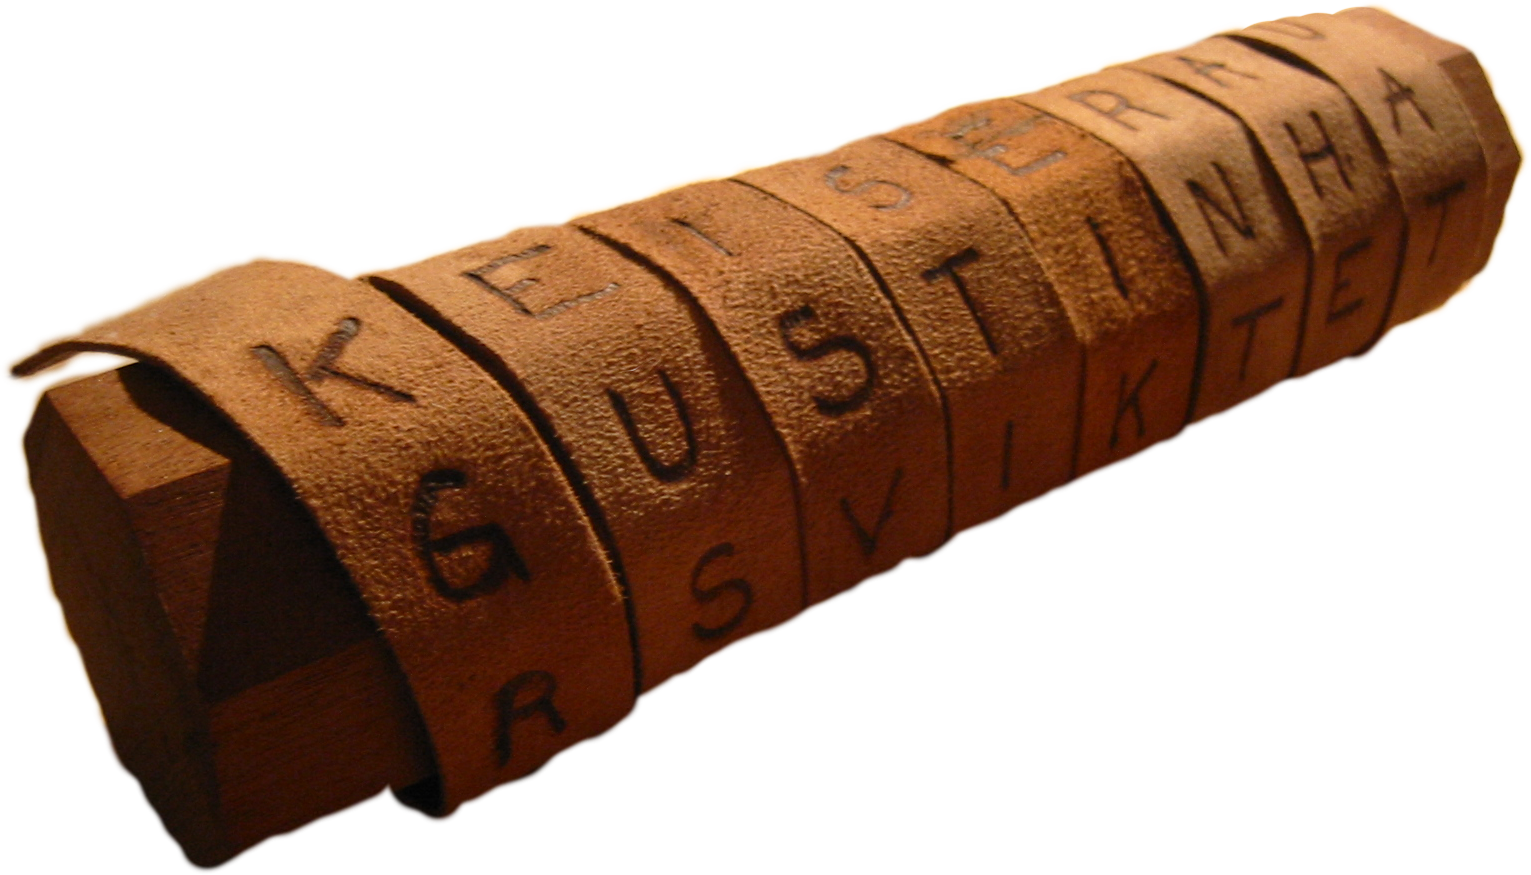
\includegraphics[scale=0.3]{img/krypto_skytale.png}\\
ein Skytale (Quelle: http://de.wikipedia.org/wiki/Skytale)
\end{center}

Ein weiteres monoalphabetisches Verfahren ist die \textbf{Caesar-Verschlüsselung}. Dieses Verfahren verschob alle Buchstaben des Klartextalphabets um eine bestimmte Zahl. Der Kommunikationspartner musste über die Anzahl der Verschiebungen informiert sein, da dieser sonst den Text nicht entschlüsseln konnte. Der Schlüssel, also die Anzahl der Verschiebungen, musste dem Kommunikationsparnter über einen sicheren Kanal übermittelt werden. [107]\\

Die Tauschchiffre ist eine verbesserte Variante des Caesar-Verfahren. Die Buchstaben des Alphabets werden mit Zahlen dargestellt und der Buchstabe A wird meistens mit 1 dargestellt, B mit 2, X mit 25 und Z mit 0. Nun wird statt einer Addition die Buchstaben mit einer Geheimzahl multipliziert. Die Geheimzahl muss aber mit der Anzahl der möglichen Buchstaben teilerfremd sein, da sonst Kollisionen entstehen. Eine Kollision tritt auf, wenn zwei verschiedene Buchstaben gleich verschlüsselt werden. Kollisionen sind zu vermeiden, da sonst der Cipher-Text nicht mehr entschlüsselt werden kann. Bei 26 Buchstaben können wir zum Beispiel 3 als Geheimzahl nehmen. Als letztes müssen wir noch einen Modulus durchführen, damit das Ergebnis der Multiplikation auf das Alphabet mit 26 Buchstaben abgebildet wird. Dieses Verfahren ist deutlich schwieriger zu Entschlüsseln als die Caesar-Verschlüsselung. Jedoch kann dieses Verfahren auch über Häufigkeitsberechnungen entschlüsselt werden, da jeder Buchstabe gleich verschlüsselt wird. [107]\\

\begin{center}
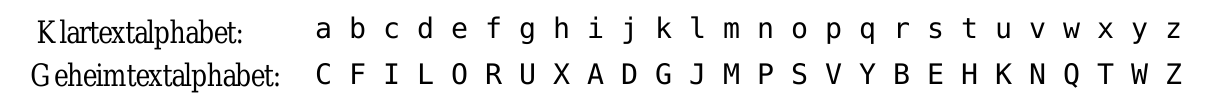
\includegraphics[scale=0.35]{img/tauschchiffre.png}\\
Anwendung der Tauschchiffre (Quelle: [107])
\end{center}

Eine andere Art von monoalphabetische Chiffre sind die Schlüsselwörter. Für die Verschlüsselung wird ein Schlüsselwort und Schlüsselbuchstabe definiert. Nun werden gleiche Buchstaben aus dem Schlüsselwort herausgenommen und das Schlüsselwort wird in das Klartextalphabet an der Stelle des Schlüsselbuchstabe hineingesetzt. Die im Schlüsselwort enthaltenen Buchstaben müssen aus dem Klartexalphabet herausgenommen werden, weil sonst Kollisionen entstehen. Nun können Wörter in das neue Alphabet übersetzt werden. [107]

\begin{center}
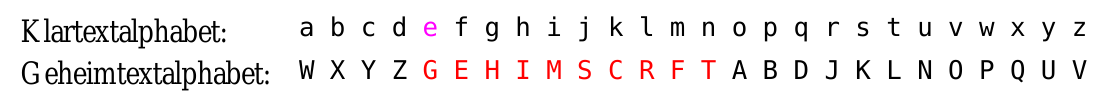
\includegraphics[scale=0.38]{img/schluesselwortes.png}\\
Anwendung des Schlüsselwortes (Quelle: [107])
\end{center}

\newpage
\paragraph{Polyalphabetische Chiffrierung}

Die \textbf{Vigenère-Chiffre} wurde 1586 von dem Franzonsen \textbf{Blaise de Vigenère} in die Welt gesetzt. Damit man einen Text verschlüsseln konnte, brauchte man als erstes ein Schlüsselwort und das Vigenère-Quadrat. In der ersten Zeile des Quadrats sind alle Buchstaben des Alphabets aufgelistet, beginnent mit A. In der zweiten Zeile ist das Alphabet aus der ersten Zeile um eine Stelle nach links verschoben, sodass der erste Buchstabe B ist. In der letzten Zeile ist der erste Buchstabe das Z. Nun wird das Schlüsselwort unter dem Klartext geschrieben und falls notwendig wiederholt. [107]\\

\begin{center}
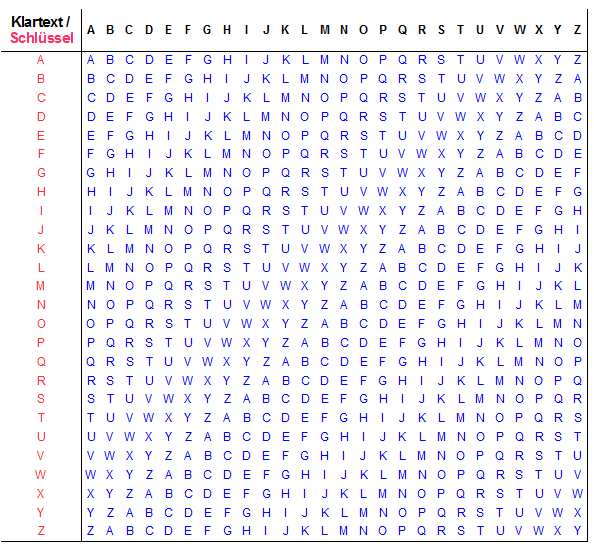
\includegraphics[scale=0.5]{img/vigere_quadrat.png}\\
das Vigenère-Quadrat (Quelle: http://www.inf-schule.de/kommunikation/kryptologie/historischechiffriersysteme/station\_onetimepad)
\end{center}

Angenommen 'JamesBond' wäre das Schlüsselwort und man möchte 'Der abgeschlossene Roman' verschlüsseln, dann müssten man das Schlüsselwort wiederholend über den Klartext schreiben. Der erste Buchstabe des Schlüsselwortes ist das J und der erste Buchstabe des Klartextes ist das D. Nun sucht man den Buchstaben in der Spalte D und der Zeile J. Dieser Buchstabe ist in diesem Beispiel der Buchstabe M. Man bemerkt schnell den Vorteil der polyalphabetischen Chiffrierungen: die Verschlüsselung eines Buchstaben hängt nicht nur von ihm ab, sondern auch von der Position des Buchstaben, da der Buchstabe des Schlüsselwortes auch relevant ist. [107]

\begin{center}
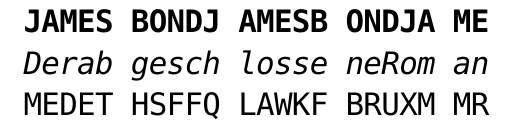
\includegraphics[scale=0.5]{img/vingere.png}\\
Schlüsselwort, Plaintext und der Ciphertext (Quelle: Einführung in die Kryptologie - Tino Hempel, \cite{krypto01})
\end{center}

Eine andere sehr bekannte polyalphabetische Chiffrierung ist die \textbf{Enigma}. Sie wurde von den Deutschen nach dem Ersten Weltkrieg entwickelt, um die Funksprüche zu verschlüsseln. Die Enigma war eine umgebautet Schreibmaschine mit drei Walzen, die je nach setzten der Kontakte den Klartext verschlüsselten. Da sich die Walzen nach jeder Eingabe weiterdrehen, werden gleiche Buchstaben nicht gleich verschlüsselt. Die Alliierten konnten den Enigma-Code durch die Turing-Bombe entschlüsseln.

\begin{center}
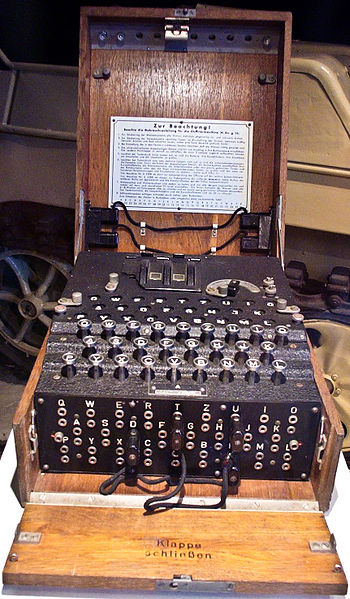
\includegraphics[scale=2.5]{img/enigma.jpg}\\
die Enigma (Quelle: http://de.wikipedia.org/wiki/Enigma\_\%28Maschine\%29)
\end{center}

\subsubsection{Moderne Kryptographie}

\subsection{Ziele der Kryptographie}

Kryptographische Systeme, die in der heutigen Zeit eingesetzt werden, müssen folgende Schutzziele einhalten, da sonst die Sicherheit der Informationen nicht gegeben ist: [108]

\begin{itemize}

\item \textbf{Vertraulichkeit} / \textbf{Zugriffschutz} (Englisch: confidentiality): Die Vertraulichkeit der Informationen ist dann gegeben, wenn der Inhalt bzw. die Aussage der Informationen vor unbefugte Personen gesichert ist. Der Wert der Informationen soll sichergestellt werden.

\item \textbf{Integrität} / \textbf{Änderungsschutz}  (Englisch: integrity): Integrität sagt aus, dass die Daten auf dem Weg zum Empfänger nicht verändert werden können. Auch wenn der Inahlt der Informationen unbekannt ist, darf die Aussage der Informationen nicht durch die Veränderung des verschlüsselten Textes änderbar sein.

\item \textbf{Authentizität} / \textbf{Fälschungsschutz} (Englisch: authenticity): Authentizität gibt an, dass ein Kommunikationspartner seine Echheit beweisen kann. Der Kommunikationspartner kann beweisen, dass er der ist für den er sich ausgibt.

\item \textbf{Verbindlichkeit} / \textbf{Nichtabstreitbarkeit} (Englisch: non repudiation): Die Verbindlichkeit besagt, dass ein Kommunikationsparnter seine gesendeten Informationen nicht abstreiten kann.
\end{itemize}

\subsection{Methoden}

\subsubsection{Klassische Methoden}

Methoden die nur mit Buchstaben oder Buchstabengruppen arbeiten, werden als 'Klassische Methoden' bezeichnet. Diese Methoden sind veraltet und unsicher.

\paragraph{Transposition}

Buchstaben des Klartextes werden anders angeordnet (siehe Skytale).

\paragraph{Substitution}

Die Buchstaben werden durch andere Buchstaben oder Symbole ersetzt (siehe Monoalphabetische Chiffrierung und Polyalphabetische Chiffrierungen).

\subsubsection{Moderene Methoden}

Moderne Methoden arbeiten mit Bits und nicht mit Buchstaben, daher können alle Arten von Binärdaten ver- und entschlüssetlt werden. Diese Methoden lassen sich in zwei große Gruppen aufteilen: die symmetrischen Verschlüsselungsmethoden und die asymmetrischen Verschlüsselungsmethoden.

\paragraph{Symmetrische Verschlüsselungsmethoden}

Symmetrische Verschlüsselungsmethoden sind einfache Bit-Operationen (z.B. XOR), Substitutions-Tabellen und andere Möglichkeiten Inforamtionen zu modifizieren. Dises Methoden sind sehr leicht umzusetzten und können leicht in Hardware implementiert werden.

\paragraph{Asymmetrische Verschlüsselungsmethoden} 

Asymmetrische Methoden basieren auf spezielle Probleme bei der Berechnung von diskrete mathematische Strukturen, wie zum Beispiel elliptische Kurven.

\subsection{Verschlüsselungsverfahren}

Heute teilt man die verschiedenen kryptographischen Systemen grob in zwei verschiedene Verfahren ein: die symmetrischen und asymmetrischen Verschlüsselungsvefahren.

\subsubsection{Symmetrische Verschlüsselungsverfahren}

Symmetrische Verschlüsselungsverfahren charakterisieren sich dadurch, dass bei der Ver- als auch bei der Entschlüsselung jeweils der gleiche Schlüssel verwendet wird. Diese Verfahren sind im Vergleich zu asymmetrischen Verfahren deutlich performanter und werden daher bei der Verschlüsselung von größeren Datenmengen verwendet. [113]\\

\begin{center}
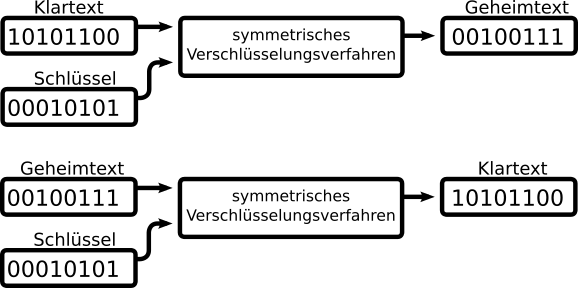
\includegraphics[scale=3]{img/sym.png}\\
der Ver- und Entschlüsselvorgang der symmetrischen Verschlüsselungsverfahren
\end{center}

Bei den symmetrischen Verschlüsselungsverfahren gibt es zwei Möglichkeiten der Verwendnung: als Stromverschlüsselung oder Blockverschlüsselung.\\
Die \textbf{Stromverschlüsselung} (oder auch Stromchiffre) verschlüsselt ganze Zeichen aus dem Klartext. Der Vorteil dieser Verschlüsselungen ist, dass der Klartext sofort verschlüsselt oder entschlüsselt werden kann. Dies ist speziell bei Echtzeitübertragungen ein klarer Vorteil.\\
Die \textbf{Blockverschlüsselung} kann nur einen Block von Daten verschlüsseln. Die Blocklänge hängt vom Verschlüsselungsalgorithmus ab, muss aber immer gleich lang sein. Damit nun ein Datenstrom verschlüsselt werden kann, benötigt man einen Betriebsmodus, der angibt, wie die Blöcke untereinander verschlüsselt werden sollen. Zudem benötigt man einen sogenannten \textbf{Padding}. Der Padding wird dann eingesetzt wenn die zu verschlüsselnte Nachricht nicht genau in ganze Blöcke eingeteilt werden kann. Mithilfe des Paddings wird die Nachricht, falls notwendig, auf einen neuen vollen Block aufgefüllt. Dies muss bei der Ver- als auch bei der Entschlüsselung beachtet werden.\\

Diese vier Blockbetriebsarten werden in der 'international Standard ISO 10116' definiert:

\begin{itemize}
\item \textbf{ECB-Mode} (Electrion Codebook Mode): Bei dieser Art der Blockverschlüsselung werden die einzelnen Blöcke unabhängig voneinander ver- und entschlüsselt. Der große Nachteil dieses Betriebsmodus ist, dass gleiche Blöcke gleich Verschlüsselt werden.

\begin{center}
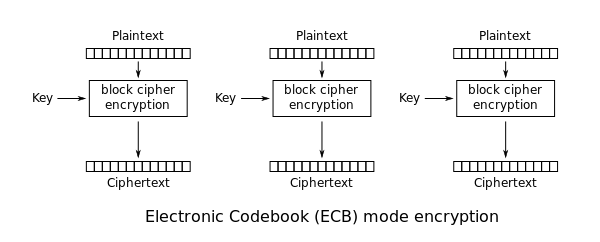
\includegraphics[scale=0.7]{img/ecb.png}\\
der Verschlüsselungsvorgang bei ECB (Quelle: http://de.wikipedia.org/wiki/Electronic\_Code\_Book\_Mode)
\end{center}

\item \textbf{CBC-Mode} (Cipher Block Chaining Mode): Diese Variante verschlüsselt einen Block mit dem vorherigen Block. Nun werden die gleiche Blöcke nicht immer gleich verschlüsselt, da der Verschlüsselungsvorgang den vorherigen Block einbezieht.

\begin{center}
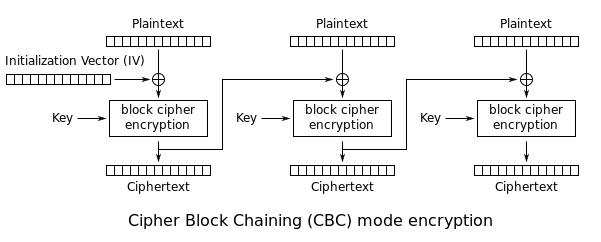
\includegraphics[scale=0.7]{img/cbc.png}\\
der Verschlüsselungsvorgang bei CBC (Quelle: http://de.wikipedia.org/wiki/Cipher\_Block\_Chaining\_Mode)
\end{center}

\item \textbf{CFB-Mode} (Cipher Feedback Mode): Dieser Betriebsmodus funktioniert ähnlich wie der CBC-Modus, jedoch wird der lesbare Block mit der Ausgabe des Verschlüsselungs Blocks bitweise XOR verknüpft.

\begin{center}
\includegraphics[scale=0.7]{img/cfb.png}\\
der Verschlüsselungsvorgang bei CFB (Quelle: http://de.wikipedia.org/wiki/Cipher\_Feedback\_Mode)
\end{center}

\item \textbf{OFB-Mode} (Output Feedback Mode): Dieser Modus ist genau gleich wie der CFB-Mode, nur dass die XOR-Verknüpfung keine Auswirkungen auf den nächsten Block hat.

\begin{center}
\includegraphics[scale=0.7]{img/ofb.png}\\
der Verschlüsselungsvorgang bei OFB (Quelle: http://de.wikipedia.org/wiki/Output\_Feedback\_Mode)
\end{center}

\end{itemize}

\subsubsection{Asymmetrische Verschlüsselungsverfahren}

Asymmetrische Methoden benötigen für die Ent- und Verschlüsselung verschiedene Schlüssel. Diese Schlüssel werden mit \textbf{Public-Key} (=öffentlicher Schlüssel) und \textbf{Private-Key} (=privater Schlüssel) bezeichnet. Falls die Information mit dem Public-Key verschlüsselt wurden, ist eine Entschlüsselung nur mithilfe des Private-Key möglich. Werden die Informationen jedoch mit dem Private-Key verschlüsselt, ist eine Entschlüsselung nur mit dem Public-Key mehr möglich.\\
Einen der beiden Schlüssel muss für die Verwendung veröffentlich werden, damit eine Kommunikation möglich ist. Welcher der beiden Schlüssel veröffentlich wird, ist irrelevant, da die zwei Verschlüsselungsmöglichkeiten beidseitig funktionieren. Der Schlüssel, den man veröffentlicht, wird in der Praxis als der Public-Key bezeichnet. [114]\\

\begin{center}
\includegraphics[scale=3]{img/asym.png}\\
der asymmetrische Verschlüsselungsvorgang
\end{center}

Da der öffentliche Schlüssel veröffentlicht wurde, können nun verschiedene Kommunikationspartner ihre Informationen mit ihm verschlüsseln und an den Inhaber des privaten Schlüssels senden. Nur der Inhaber des privaten Schlüssel ist imstande die Daten zu entschlüsseln.\\
Die zweite Möglichkeit, die mit diesem Verfahren möglich ist, ist das der Inhaber des Private-Key eine Nachricht mit seinem Schlüssel verschlüsselt und an alle Kommunikationspartner überträgt. Da die Kommunikationspartner die Nachricht fehlerfrei entschlüsseln können, muss der Sender im Besitz des privaten Schlüssels sein. Damit ist die Echtheit der Indentität des Kommunikationspartners sichergestellt (digitale Unterschrift).\\
Für eine beidseitige Übertragen mithilfe eines asymmetrischen Verfahren werden zwei unabhängige Schlüsselpaare benötigt. Beide Kommunikationsparnter müssen ihre öffentlichen Schlüssel veröffentlichen und auf ihren privaten Schlüssel achtgeben.

\paragraph{Digitale Signaturen}

Eine digitale Signatur (=digitale Unterschrift) ist eine Methode basierend auf den asymmetrischen Verschlüsselungsmethoden, die die Integrität und Nichtabstreitbarkeit im Netzwerk sicherstellt. Eine digitale Signatur kann nur mit dem Private-Key erzeugt werden und die Entschlüsselung daher nur mit dem Public-Key. Kann die Signatur entschlüsselt werden, so weiß man, dass der Sender im Besitz des Privaten SChlüssels ist und derjenige ist für den er sich ausgibt. \cite{wiki03}

\paragraph{Digitale Zertifikate}

Digitale Zertifikate sind Ansammlungen von Daten, die mithilfe von kryptographischen Methoden Authenzität und Integrität der enthaltenen Informationen sicherstellen. Der weitverbreitete X.509-Zertifikat Standard z.B. bestätigt die Intentität des Inhabers, Richtigkeit des öffentlichen Schlüssels und nocht weiteren Informationen. Einige Zertifikate (Root-Zertifikate) haben die Möglichkeit andere Zertifikate zu unterschreiben. Wenn man nun das Root-Zertifikat vertraut, vertraut man automatische alle Zertifikate, die von diesem Zertifikat unterschrieben worden sind.

\subsubsection{Hybride Verschlüsselungsverfahren}

\textbf{Hybride Verschlüsselungsverfahren} sind kryptographische Verfahren, die asymmetrische und symmetrische Verschlüsselungsverfahren in Kombination einsetzten. Da die Übermittlung des Schlüssels allein mit symmetrischen Verfahren nicht möglich ist, da der Schlüssel im Klartext übertragen wird, verlassen sich hybride Verfahren bei dem Schlüsselaustausch (=key-exchange) auf asymmetrische Verschlüsselungssysteme. [115]

\subsubsection{Hash-Verfahren}

Eine \textbf{Hashfunktion} ist eine Funktion, die eine beliebige Menge an Eingangsinformationen auf eine fixe Länge an Ausgangsinformationen abbildet.  Das Ziel von Hashfunktionen ist das Erschweren der Suche nach Kollisionen. Kollisionen können bei Hashfunktionen nicht verhindert werden, weil die Länge der Eingangsinformationen größer als die Länge der Ausgangsinformationen sein kann. Ein weiteres Ziel von Hashfunktionen ist das Verhindern der Möglichkeit des Rückrechnens, also die Ermittlung der Eingangsgröße aus der Ausgangsgröße.[111]

\newpage
\section{Kryptoanalyse}

Die Krytpoanalyse beschäftigt sich mit Methoden und Techniken aus einem verschlüsselten Text Informationen zu gewinnen. Sie ist das Gegenstück zur Kryptographie und versucht das kryptographische System durch die Anwendung von bestimmten Methoden zu umgehen. [109]

\subsection{Ziele der Kryptoanalyse}

Das oberste Ziel der Kryptoanalyse ist die Ermittlung des Schlüssels, um an den Wert der Informationen zu gelangen. Damit die Kryptoanalyse das Ziel erreichen kann, muss das kryptographische System unwirksam gemacht werden, entweder durch ausprobieren des Schlüssels oder anderen Methoden. Oftmals ist das Knacken des kryptographischen Systems für die Ermittlung des Schlüssels gar nicht notwendig, da die falsche Anwendung des Systems, schwache Passwörter usw. meistens ausreichen, das kryptographische System zu umgehen. [109]

\subsection{Methoden}

\paragraph{Brute-Force-Methode} Bei dieser Art von Angriff werden alle möglichen Schlüssel ausprobiert. Dabei werden Schlüssel, die wahrscheinlich häufiger auftreten, als erstes ausprobiert. Oftmals ist nicht das Verschlüsselungssystem die Schwäche, sondern zu einfache gewählte Passwörter. Durch die Annahme, das der verwendete Schlüssel kurz und eine Kombination aus Wörtern und Zahlen ist, kann in den meisten Fällen der Schlüssel erraten und das Verschlüsselungssystem umgangen werden.

\paragraph{Wörterbuchangriff} Diese Methoden verwenden große Schlüsselsammlungen aus mehreren verschiedenen Sprachräumen und kann einfache Passwörter, die nur aus einem Wort bestehen, mit leichtigkeit Knacken.

\paragraph{Man-in-the-middle-Angriff} Der Angreifer sitzt zwischen den Kommunikationspartner und kann die Informationen in Klartext mitlesen und verändern.

\paragraph{...} Es gibt noch zahlreiche andere Methoden, doch auf die werden hier nicht mehr eingegangen. 

\section{Heutige Verschlüsselungsverfahren}

\subsubsection{Nennenswerte symmetrische Verschlüsselungssysteme}

\paragraph{DES}

DES wurde 1975 von IBM veröffentlicht und basierte auf den Verschlüsselungsalgorithmus namens 'Lucifer'. DES verwendet für die Verschlüsselung einen 64 Bit langen Schlüssel, jedoch werden 8 davon als Prüfsumme verwendet. Dieses Verschlüsselungsverfahren ist nicht mehr sicher, da die heutigen Computer die 56 bit langen Schlüssel mit Brute-Force-Attacken innerhalb weniger Stunde knacken können. [116]

\paragraph{3DES}

Triple DES ist der Nachfolger des DES-Standarts und wendet für die Ver- und Entschlüsselung DES dreimal an. Hierbei verwendet das Verfahren zwei 64 Bit lange Schlüssel, die abwechselend eingesetzt werden. Jedoch werden von den zwei 64 Bit langen Schlüssel bei dem Verfahren nur 112 Bit effektiv eingesetzt, da die restlichen Bits für Prüfzwecke benötigt werden. Dieses Verfahren gilt grundsätzlich noch als sicher, doch es wird drigenst geraten auf einen Ersatz umzusteigen. [117]

\paragraph{AES}

AES, der ausgewählte Nachfolger von DES, wurde im Oktober 2000 vom 'National Institute of Standards and Technology' als neuer Standard freigegeben. AES ist ein Blockchiffre und kann für die Verschlüsselung 128, 160, 192, 224 oder 256 Bit langen Schlüssel verwenden. Bis heute ist der AES-Standard nocht im Gebrauch und auch immer noch kryptographisch sicher. [118]

\subsection{Asymmetrische Verschlüsselungsverfahren}

\subsubsection{Nennenswerte asymmetrische Verschlüsselungssysteme}

\paragraph{Diffie-Hellman}

Diffie-Hellman ist ein Austauschprotkoll, welches den Austausch eines geheimen Schlüssels erlaubt. Es ist praktisch unmöglich aus den gesendeten Informationen den Schlüssel zu berechen - dieses Problem wird als das Diffie-Hellman-Problem bezeichnet. [119]

\paragraph{RSA}

RSA (Rivest-Shamir-Adleman) wird für Verschlüsselungen und digitale Signaturen verwendet. [120]

\subsection{Hybride Verschlüsselungsverfahren}

\subsubsection{Merkmale}

Hybride Verschlüsselungssysteme nutzen die Vorteile der symmetrischen und asymetrischen Systeme aus. Bei diesen Verfahren wird ein geheimer Schlüssel zwischen den Parntern mithilfe eines asymmetrischen Systems ausgemacht. Dieser Vorgang ist oftmals sehr rechenintensiv und wird daher nur einmal pro Sitzung durchgeführt. Nachdem der Schlüssel ausgetauscht wurde wird mit einem symmetischen System gearbeite, da diese sehr viel weniger Leistung vüf die Ver- und Entschlüsselungen benötigen. [115]

\subsubsection{Nenneswerte hybride Verschlüsselungssysteme}

\paragraph{IPsec}

IPsec ist eine Ansammlung an Protokollen und Verschlüsselungssystemen, die modular verwendet werden können. IPsec kapselt und verschlüsselt gewöhnliche IP-Pakete. IPsec versucht die Lesbarkeit, Manipulation oder Weiterleitung von Paketen zu verhindern. Mit IPsec können Netzwerkgeräte, die die Pakete weiterleiten, nicht sehen an wen oder von wem die gesendeten Paket kommen.

IPsec ist eine Ansammlng an verschiedenen Protokollen und Verschlüsselungssystemen, die modular verwendet werden können. IPsec kapselt und verschlüsselt IP-Pakete, damit die Pakete nicht von Netzwerkgeräten umgeleitet, gelesen oder geändert werden können. Zudem ist es für ein Netzwerkgerät dazwischen unmöglich zu ermitteln, wer das Paket verschickt hat bzw. wer das Paket empfängt. [121]

\paragraph{TLS/SSL}

TLS steht für \textbf{Transport Security Layer} (alte Bezeichnung: SSL, Secure-Socket-Layer) und wird bei HTTPS eingesetzt. [122]

\paragraph{PGP}

PGP steht für \textbf{Pretty-Good-Privacy} und ist ein Programm, welches die Verschlüsselung und Entschlüsselung von Daten erlaubt. Wird in der Praxis für das Ver- und Entschlüsseln von E-Mails verwendent. [123]

\subsection{Hash-Verfahren}

\paragraph{MD5}

MD5 steht für \textbf{Message-Digest Algorithm 5} und gibt bei beliebiger Eingangsgröße einen 128 Bit langen Hashwert aus. Diese Methode wird oft für die Bestätigung der Vollständigkeit von Daten verwendet und ist heute nicht mehr für den Einsatz zu empfehlen. [124]

\paragraph{SHA}

SHA steht für \textbf{Seucre-Hash-Algorithm} und ist eine Ansammulung von mehreren standarisierte Hashverfahren, die heute für digitale Signaturen und Prüfsummen verwendet werden. [125]

\part{Programmrealisierung}

\chapter{Schnittstellen (Alin Porcic / Manpreet Singh)}

\section{CLI (Alin Porcic)}
\lfoot{Alin Porcic}

\subsection{Allgemeines}

Das Programm bietet eine integrierte textbasierende Schnittstelle für die primäre Verwendung an. Der Syntax der CLI-Eingaben setzen sich aus drei Bestandteile zusammen: dem Hauptbefehl, den Parametern und den Argumenten. Jede Eingabe muss einen Hauptbefehl definieren und darf nicht mehrere definieren. Jeder Hauptbefehl kann mehrere Parameter definieren und jeder dieser Parameter kann Argumente definieren. Die CLI unterscheidet die Parameter in obligatorische und optionale Parameter. Die obligatorischen Parameter müssen angegeben werden, da sonst die Ausführung des Befehles nicht erfolgen kann. Die optionalen Parameter hingegen können weggelassen werden. Die Anordnung der Parameter und Argumente ist für die diese CLI-Implementierung irrelevant.\\

Nach dem Drücken der ENTER-Taste wird die CLI-Eingabe eingelesen und interpretiert. Ist die Interpretation der Eingabe nicht möglich, da zum Beispiel ein Paramter mehrfach definiert wurde, wird eine Fehlermeldung in roter Farbe ausgegeben. Einige Fehlermeldungen, die ausgegeben werden können, sind zum Beispiel:

\begin{itemize}
\item \textbf{Command not found}: Befehl ist nicht definiert und kann nicht ausgeführt werden.
\item \textbf{Parameter not found}: Der Befehl existiert, doch der angeführte Parameter für diesen Befehl existiert nicht.
\item \textbf{Argument could not be parsed}: Das eingegeben Argument konnte nicht in ein Objekt umgewandelt werden.
\item ...
\end{itemize}

Mit der linken und rechten Pfeiltaste kann die Position des Cursors im Eingabefeld verändert werden und mit der Backspace-Taste (Rücktaste) kann ein Zeichen in der Eingabe entfernt werden. Die CLI führt eine History über die zuletzt eingegebenen Befehle. Mit der Oben- und Unten-Taste können die Einträge der History in das Eingabefeld eingesetzt werden.

\subsection{Programmstruktur}

Die CLI ist programmtechnisch einfach aufgebaut: CLIInput, CLIFramework und CLIOutput. Die CLIInput-Komponente hat die einfache Aufgabe, die Eingabe einzulesen. Dabei soll der Cursor verschiebbar sein und eine History mit den zuletzt eingegebenen Befehle gesammelt werden.\\
Nachdem die Eingabe-Zeile eingelesen wurde, übernimmt das CLIFramework den schwierigen Teil: das Interpretieren. Es wird versucht, die einzelnen Parameter und deren Argumente aus dem Text zu lesen, diese in Objekte umwandeln und zu überprüfen ob der Befehl überhaupt ausführbar ist. Falls die Ausführung nicht möglich ist, da ein obligatorischer Parameter fehlt oder die Argumente eines Parameters fehlen, muss das CLIFramework die passende Fehlermeldung zurückgeben und die Ausführung verweigern.\\
Das CLIFramework spricht den Benutzer über die CLIOutput-Komponente an. Diese Komponente muss sogenannte 'Color-Tags' (also Farbmarkierungen) aus dem Text lesen können und diese mit den entsprechenden Farben ersetzen. Zum Beispiel muss der String '\textless color\textgreater \textless blue\textgreater EinText' in Blau geschrieben werden.

\begin{center}
\includegraphics[scale=2.0]{img/mad_cli.png}\\
Funktionsweise der CLI
\end{center}

\subsection{Probleme und Beschränkungen}

Bei der CLI tauchten einige Probleme bei der Eingabe von Befehlen auf. Das .NET-Framework bietet eine Möglichkeit zeilenweise Eingaben einzulesen und dabei kann die Position des Cursors geändert werden. Bei Linux ist leider dies mit Mono leider nicht möglich und daher musste eine eigene Methode entwickelt werden, die zeilenweise Eingaben einlesen kann. Es soll auch die Möglichkeit bestehen den Cursor zu verändern oder eine History aufzurufen.\\
Ein weiteres Problem bei der Implementierung ist, dass das Eingabefeld nicht über mehrere Zeilen gehen kann. Dies konnte aus programmtechnischen Schwierigkeiten nicht realisiert werden.
Es ist auch nicht möglich, interaktive Befehle für die CLI zu schreiben, da der CLI-Server diese Funktionalität nicht unterstützt.

\section{CLI-Server und CLI-Client (Alin Porcic)}
\lfoot{Alin Porcic}

Über den CLI-Server und CLI-Client ist es möglich die textbasierte Schnittstelle über einen Netzwerkservice anzusprechen. Nachdem eine erfolgreiche Verbindung aufgebaut wurde, kann der Client die Befehle lokal einlesen und an den Server senden. Dieser versucht den empfangenen Befehl zu interpretieren und schick die Ausgabe wieder zurück. Die CLI als Dienst funktioniert genau gleich wie die lokale CLI. Der Unterschied ist nur, dass die Interpretation und Ausführung nicht lokal geschieht, sondern auf dem Server. 

\begin{center}
\includegraphics[scale=2.0]{img/mad_client_session.png}\\
Funktionsweise der CLI-Server/Client (CLISession ist mit CLI-Server gleichzustellen)
\end{center}

\section{CLI-Server}

Der CLI-Server wartet auf einkommende TCP-Verbindungen und bearbeitet die Anfragen. Die Kommunikation zwischen Server und Client wird mit AES256 verschlüsselt ohne Schlüsselaustausch, das heißt, falls die Anfrage des Clients vom Server nicht sofort entschlüsselt werden kann, weil der AES-Schlüssel falsch ist, wird die Verbindung abgebrochen. Zudem kann der Server nur einen Nutzer gleichzeitig bearbeiten.\\
Am Beginn der Kommunikation sendet der Server dem Client seine Versionsnummer und Servername. Anhand von diesen Informationen kann der Client entscheiden ob er sich mit diesen Server verbinden möchte. Da diese Informationen schon verschlüsselt sind, kann der Client davon ausgehen, dass er mit dem Server kommuniziert. Der AES-Schlüssel wird auf der Serverseite in der Konfigurationsdatei im Klartext abgespeichert und ist mit einem einfachen Text-Editor änderbar.\\

\section{CLI-Client}

Der CLI-Client verbindet sich auf den Server-Dienst und vergibt Anfragen. Wie bereit oben schon erwähnt, wird sofort nach dem TCP-Handshake in AES verschlüsselt. Der CLI-Client liest den AES-Schlüssel aus seiner lokalen Konfiguration und ist daher auch im Klartext abgespeichert.

\newpage
\section{GUI (Manpreet Singh)}
\lfoot{Manpreet Singh}
Nach einigen Startschwierigkeiten beim Entscheiden, wer nun diesen Abschnitt programmiert, ist schlussendlich mir die Aufgabe zuteilgeworden.\\\\
Dieser Teil ist meines Erachtens nach eine besonders große Herausforderung. Das Problem bestand darin, den verschiedenen Anforderungen gerecht zu werden. Manche legen Wert auf Effizienz wohingegen andere mehr auf die Optik achten.\\\\
Nach 3 Versuchen klappte es eine graphische Benutzeroberfläche zu programmieren, die alle geforderten Aspekte erfüllte.\\

\subsection{Versionen und ihre Probleme}
\subsubsection{Version 1}
\begin{center}
\includegraphics[scale=0.5]{../docs/lyaton/graphics/GUI_v1_start.png}\\
\textbf{Startfenster}
\end{center}
\begin{center}
\includegraphics[scale=0.5]{../docs/lyaton/graphics/GUI_v1_nodes.png}\\
\textbf{Nodes-Fenster}
\end{center}
Die Arbeit and dieser Version wurde bald eingestellt. Diese Version ist rückblickend zu einem 'Testobjekt' geworden. Allerdings habe ich wertvolle Erfahrung gesammelt und hatte meinen ersten Kontakt mit Visual C\#.
\subsubsection{Version 2}
\begin{center}
\includegraphics[scale=0.65]{../docs/lyaton/graphics/GUI_v2_config.png}\\
\textbf{Konfigurationsfenster}
\end{center}
Leider wurde mir erst viel zu spät bewusst, dass ich mich in etwas viel zu aufwendiges verstrickt hatte. Meine Herangehensweise war vollkommen falsch. Ich habe viel zu groß gedacht. Der richtige Ansatz bei solchen Projekten, die einem endlose Möglichkeiten bieten, ist es klein anzufangen. 
Durch diese neu gewonnene Erfahrung fiel mir der Umgang mit C\# immer einfacher.
\subsubsection{Version 3 - Final Version}
\begin{center}
\includegraphics[scale=0.65]{../docs/lyaton/graphics/GUI_v3_demo.png}\\
\textbf{Hauptfenster}
\end{center}
Diese Version ist kurz und bündig. Sie erfüllt die gewünschten Anforderungen und ist dabei optisch ansprechend. Ich wollte mehr Features, wie z.B. Graphen zur Anzeige vom Netzwerkverkehr, implementieren. Das war jedoch zeitlichen Gründen nicht mehr realisierbar.\\

Alles in Allem kostete mich das Programmieren der Benutzeroberfläche viel Zeit und Geduld. Jedoch kann ich mit Sicherheit sagen, dass ich viel Erfahrung gesammelt habe, die mir auf meinem weiteren Lebensweg helfen wird.

\subsection{Technische Realisierung}
Die graphische Oberfläche wurde mit Hilfe von Microsoft Visual Studio programmiert. Dieses IDE bietet die Möglichkeit, dass alles graphisch zusammengebaut werden kann und Windows für einen den dazu gehörigen Initialisierungscode auto-generiert. Dieser Code beinhaltet die Deklaration und die vom Standard abweichenden Parameter. \\
\begin{center}
\includegraphics[scale=0.5]{../docs/lyaton/graphics/Real_IDE.png}
\begin{scriptsize}
\textbf{Graphischer Baukasten in Visual Studio} - MainWindow.cs
\end{scriptsize}
\end{center}
\textbf{Ausschnitt - Windows generierter Code}
\begin{lstlisting}
// 
// MainWindow
// 
this.AutoScaleDimensions = new System.Drawing.SizeF(6F, 13F);
this.AutoScaleMode = System.Windows.Forms.AutoScaleMode.Font;
this.ClientSize = new System.Drawing.Size(884, 562);
this.Controls.Add(this.panelInformation);
this.Controls.Add(this.labelLastReloadTime);
this.Controls.Add(this.labelLastReloadTimeTitle);
this.Controls.Add(this.labelConfigStatus);
this.Controls.Add(this.labelConfigStatusTitle);
this.Controls.Add(this.buttonReload);
this.Controls.Add(this.listBoxNodes);
this.Controls.Add(this.panelSeperator);
this.Controls.Add(this.panelTop);
this.FormBorderStyle = System.Windows.Forms.FormBorderStyle.FixedSingle;
this.Icon = ((System.Drawing.Icon)(resources.GetObject("$this.Icon")));
this.MaximizeBox = false;
this.Name = "MainWindow";
this.ShowIcon = false;
this.StartPosition = System.Windows.Forms.FormStartPosition.CenterScreen;
this.Text = "MAD - Networkmonitoring | Nodes";
this.FormClosing += new
	System.Windows.Forms.FormClosingEventHandler(this.MainWindow_FormClosing);
this.panelTop.ResumeLayout(false);
this.panelTop.PerformLayout();
((System.ComponentModel.ISupportInitialize)(this.pictureBoxTopPanel)).EndInit();
this.panelInformation.ResumeLayout(false);
this.panelInformation.PerformLayout();
((System.ComponentModel.ISupportInitialize)(this.pictureBoxLightRedoff)).EndInit();
((System.ComponentModel.ISupportInitialize)(this.pictureBoxLightRedOn)).EndInit();
((System.ComponentModel.ISupportInitialize)(this.pictureBoxLightGreenOn)).EndInit();
((System.ComponentModel.ISupportInitialize)(this.pictureBoxLightGreenOff)).EndInit();
this.tableLayoutPanelInfoJobs.ResumeLayout(false);
this.tableLayoutPanelInfoJobs.PerformLayout();
this.tableLayoutPanelInfoGeneral.ResumeLayout(false);
this.tableLayoutPanelInfoGeneral.PerformLayout();
this.ResumeLayout(false);
this.PerformLayout();


\\
\\Am ende alle verwendeten Objekte
\\
private System.Windows.Forms.Panel panelTop;
private System.Windows.Forms.Label labelTopBoxTitle;
private System.Windows.Forms.PictureBox pictureBoxTopPanel;
private System.Windows.Forms.Panel panelSeperator;
private System.Windows.Forms.ListBox listBoxNodes;
private System.Windows.Forms.Button buttonReload;
private System.Windows.Forms.ToolTip toolTipNodeListing;
private System.Windows.Forms.Label labelConfigStatusTitle;
private System.Windows.Forms.Label labelConfigStatus;
private System.Windows.Forms.Label labelLastReloadTimeTitle;
private System.Windows.Forms.Label labelLastReloadTime;
private System.Windows.Forms.Panel panelInformation;
private System.Windows.Forms.Label labelInfoTitleID;
private System.Windows.Forms.Label labelInfoTitleMac;
private System.Windows.Forms.Label labelInformationTitle;
private System.Windows.Forms.Label labelInfoTitleGUID;
private System.Windows.Forms.Label labelInfoTitleName;
private System.Windows.Forms.Label labelInfoTitleState;
private System.Windows.Forms.Label labelInfoTitleIP;
private System.Windows.Forms.Label labelInfoMAC;
private System.Windows.Forms.Label labelInfoID;
private System.Windows.Forms.Label labelInfoGUID;
private System.Windows.Forms.Label labelInfoIP;
private System.Windows.Forms.Label labelInfoName;
private System.Windows.Forms.Label labelInfoState;
private System.Windows.Forms.TableLayoutPanel tableLayoutPanelInfoGeneral;
private System.Windows.Forms.ListBox listBoxInfoJobs;
private System.Windows.Forms.Label labelInfoJobsTitle;
private System.Windows.Forms.TableLayoutPanel tableLayoutPanelInfoJobs;
private System.Windows.Forms.Button buttonCLI;
private System.Windows.Forms.Panel panelSeperatorInformation;
private System.Windows.Forms.PictureBox pictureBoxLightGreenOn;
private System.Windows.Forms.PictureBox pictureBoxLightGreenOff;
private System.Windows.Forms.PictureBox pictureBoxLightRedoff;
private System.Windows.Forms.PictureBox pictureBoxLightRedOn;
private System.Windows.Forms.Label labelInfoJobsTitleID;
private System.Windows.Forms.Label labelInfoJobsTitleType;
private System.Windows.Forms.Label labelInfoJobsTitleGUID;
private System.Windows.Forms.Label labelInfoJobsTitleOutstate;
private System.Windows.Forms.Label labelInfoJobsOutstate;
private System.Windows.Forms.Label labelInfoJobsType;
private System.Windows.Forms.Label labelInfoJobsGUID;
private System.Windows.Forms.Label labelInfoJobsID;
private System.Windows.Forms.Button buttonInfo;
private System.Windows.Forms.TextBox textBoxInfoJobsMemo2;
private System.Windows.Forms.TextBox textBoxInfoJobsMemo1;
private System.Windows.Forms.Label labelInfoJobsTitleMemo2;
private System.Windows.Forms.Label labelInfoJobsTitleMemo1;
public System.Windows.Forms.Button buttonScan;
\end{lstlisting}

Zusätzlich muss die im Hintergrund ablaufende „Logik“ programmiert werden, wie zum Beispiel welches Ereignis aufgrund einer Interaktion stattfindet.\\\\
Die in der Region Logic befindliche Methode InitGUI sorgt dafür, dass das Jobsystem, die Datenbank und der DHCP Reader mitgegeben werden können.\\
\begin{lstlisting}
public partial class MainWindow : Form
    {
		public MainWindow()
        {
            InitializeComponent();
            labelConfigStatus.Text = configStatus;
        }

        #region Events

        private void buttonReload_Click(object sender, EventArgs e)
        {
            _nodes = _js.GetNodesAndJobs();
            this.listBoxNodes.Items.Clear();
            this.listBoxInfoJobs.Items.Clear();
            _countNode = 0;
            foreach(JobNodeInfo node in _nodes)
            {
                _countNode++;
                this.listBoxNodes.Items.Add(_countNode.ToString() + ".) " + node.mac);
            }
            labelLastReloadTime.Text = DateTime.Now.ToLongTimeString();
        }

        private void MainWindow_FormClosing(object sender, EventArgs e)
        {
            Application.Exit();
        }

        private void listBoxNodes_SelectedIndexChanged(object sender, EventArgs e)
        {
            this.listBoxInfoJobs.Items.Clear();

            labelInfoJobsGUID.Text = "";
            labelInfoJobsID.Text = "";
            labelInfoJobsOutstate.Text = "";
            labelInfoJobsType.Text = "";

            labelInfoMAC.Text = _nodes[listBoxNodes.SelectedIndex].mac;
            labelInfoID.Text = _nodes[listBoxNodes.SelectedIndex].id.ToString();
            labelInfoGUID.Text = _nodes[listBoxNodes.SelectedIndex].guid.ToString();
            labelInfoIP.Text = _nodes[listBoxNodes.SelectedIndex].ip.ToString();
            labelInfoName.Text = _nodes[listBoxNodes.SelectedIndex].name;
            labelInfoState.Text = _js.NodeState(_nodes[listBoxNodes.SelectedIndex].state);
            textBoxInfoJobsMemo1.Text = _nodes[listBoxNodes.SelectedIndex].memo1;
            textBoxInfoJobsMemo2.Text = _nodes[listBoxNodes.SelectedIndex].memo2;



            if (_js.NodeState(_nodes[listBoxNodes.SelectedIndex].state) == "Active")
            {
                this.pictureBoxLightGreenOn.Visible = true;
                this.pictureBoxLightGreenOff.Visible = false;
                this.pictureBoxLightRedOn.Visible = false;
                this.pictureBoxLightRedoff.Visible = true;
            }

            else
            {
                this.pictureBoxLightGreenOn.Visible = false;
                this.pictureBoxLightGreenOff.Visible = true;
                this.pictureBoxLightRedOn.Visible = true;
                this.pictureBoxLightRedoff.Visible = false;
            }

            _countJob = 0;
            foreach (JobInfo jf in _nodes[listBoxNodes.SelectedIndex].jobs)
            {
                _countJob++;
                this.listBoxInfoJobs.Items.Add(_countJob.ToString() + ".) " + jf.name);
            }
            
        }

        private void buttonCLI_Click(object sender, EventArgs e)
        {
            Logger.Log("Programm Start. CLI Start.", Logger.MessageType.INFORM);
            _CLITHREAD.Start();
            this.buttonCLI.Enabled = false;

        }

        private void listBoxInfoJobs_SelectedIndexChanged(object sender, EventArgs e)
        {
            labelInfoJobsGUID.Text =
            	 _nodes[listBoxNodes.SelectedIndex].jobs[listBoxInfoJobs.SelectedIndex].guid.ToString();
            labelInfoJobsID.Text =
            	 _nodes[listBoxNodes.SelectedIndex].jobs[listBoxInfoJobs.SelectedIndex].id.ToString();
            labelInfoJobsOutstate.Text =
            	 _nodes[listBoxNodes.SelectedIndex].jobs[listBoxInfoJobs.SelectedIndex].outstate;
            if (_nodes[listBoxNodes.SelectedIndex].jobs[listBoxInfoJobs.SelectedIndex].outstate ==
            	 "Success")
            {
                labelInfoJobsOutstate.ForeColor = Color.DarkGreen;
            }

            else
                labelInfoJobsOutstate.ForeColor = Color.DarkRed;
            labelInfoJobsType.Text =
            	 _nodes[listBoxNodes.SelectedIndex].jobs[listBoxInfoJobs.SelectedIndex].type;
        }

        private void buttonInfo_Click(object sender, EventArgs e)
        {
            _Info.ShowDialog(this);
        }

        private void buttonScan_Click(object sender, EventArgs e)
        {
            Scan();
        }

        #endregion Events

        #region Logic

        public static void InitGUI(JobSystem jobSys, DB database, DHCPReader dhcp)
        {
            _js = jobSys;
            _db = database;
            _dhcp = dhcp;

            cli = new CLI(_js, _dhcp, _db);
            _CLITHREAD = new Thread(new ThreadStart(cli.Start));
        }

        private static void Scan()
        {
            _Scan.ShowDialog();
        }

        #endregion 
                

    }
\end{lstlisting}
Weiters wichtig ist das Scan-Fenster. Dieses sorgt dafür, dass die Geräte im LAN eingelesen und aufgelistet werden. Die wichtige Methode hier ist die InvokeArpReader-Methode, sie wird aufgerufen sobald auf 'Start Scan' gedrückt wird. Sie ruft dann den ArpReader auf der dann den eigentlichen Scan durchführt.\\
\begin{lstlisting}
private void InvokeArpReader()
        {

            try
            {
                ARPReader.srcAddress = IPAddress.Parse(textBoxLocalIP.Text);
                ARPReader.netAddress = IPAddress.Parse(textBoxNetwork.Text);
                ARPReader.subnetMask = Convert.ToUInt32(comboBoxSubnetmask.SelectedItem);
                if (this.comboBoxNWD.Text != "Default")
                {
                    ARPReader.networkInterface =
                    	 Convert.ToUInt16(this.comboBoxNWD.SelectedItem.ToString()) - (uint)1;
                }

                if (checkBoxOneScan.Checked)
                {
                    ARPReader.SetWindow(this);
                    ARPReader.FloodStart();
                    _js.SyncNodes(ModelHost.hostList);
                    ARPReader.ResetWindow();
                }

                else
                {
                    ARPReader.SteadyStart(_js);
                    GUILogic.SteadyActivated = true;
                    _mw.buttonScan.Enabled = false;
                }
                validEntering = true;
            }

            catch
            {
                MessageBox.Show("Please check the fields again, your enterings seem to be incorrect",
                	 "Ups...Something went wrong", MessageBoxButtons.OK, MessageBoxIcon.Error);
                validEntering = false;
            }

            
            return;
        }
\end{lstlisting}
Die letzte wichtige Klasse der graphischen Oberfläche ist die GUILogic. Sie selbst wird als erstes von der Main aufgerufen, und dann ruft die sie selbst die InitGUI des MainWindows und des ArpScanWindows auf. Anschließend ladet sie das MainWindow.\\
\begin{lstlisting}
public static class GUILogic
    {
        public static bool SteadyActivated;
        public static MainWindow _MainWindow = new MainWindow();
        public static ArpScanWindow _ArpScanWindow = new ArpScanWindow();

        public static void RunGUI(JobSystem jobSys, DB dataBase, DHCPReader dhcp)
        {
            ArpScanWindow.InitGUI(jobSys, dataBase, _MainWindow);
            MainWindow.InitGUI(jobSys, dataBase, dhcp);
            Application.Run(_MainWindow);           
        }
    }
\end{lstlisting}
\chapter{Konfiguration (Alin Porcic)}
\lfoot{Alin Porcic}

Die Konfiguration des Programmes erfolgt über eine Konfigurationsdatei, damit das Programm auf Linux und Windows unverändert verwendet werden kann. Falls keine Konfiguration verfügbar ist, wird eine neue Konfiguration mit den Standardwerten im Verzeichnis 'data' unter dem Namen 'mad.conf' erstellt. Diese Datei beinhaltet einen JSON-String, der die Konfiguration beinhaltet. Die Änderung der Konfiguration kann mithilfe eines Texteditors durchgeführt werden. Einige Felder der Konfigurationsdatei:

\begin{itemize}
\item \textbf{LOG\_FILE\_DIRECTORY}: Der Pfad in der die Log-Datei hingeschrieben werden soll.
\item \textbf{SERVER\_HEADER}: Name des CLI-Servers.
\item \textbf{AES\_PASS}: Das AES-Passwort für die korrekte Authentifikation von Clients.
\item \textbf{SMTP\_SERVER}: SMTP-Server Adresse.
\item \textbf{SMTP\_PORT}: Port des SMTP-Servers.
\item \textbf{SMTP\_USER}: Nutzername am SMTP-Server.
\item \textbf{SMPT\_PASS}: Passwort des Accounts.
\item \textbf{MAIL\_DEFAULT}: Globale Mail-Adressen, die bei Regelbruch, anzuschreiben sind.
\item ...
\end{itemize}

\begin{center}
\includegraphics[scale=0.6]{img/madconf.png}\\
eine mögliche Konfiguration
\end{center}

\chapter{JobSystem (Alin Porcic)}
\lfoot{Alin Porcic}

\section{Allgemeines}

Das Jobsystem organisiert die Netzwerkaufgaben (oder auch Jobs) und Netzwerkgeräte (oder auch Netzwerkknoten, Knoten, Nodes) innerhalb des Programmes und bietet eine Schnittstelle an, um diese zu entfernen, hinzuzufügen oder zu konfigurieren. Das JobSystem ist nicht an einer textbasierten oder grafischen Schnittestelle gebunden, sondern kann auf Programmebene über Methodenaufrufe angesteuert werden. Alle Methodenaufrufe werden intern über Locks vor Race-Conditions und weiteren Multithreading-Problemen geschützt.\\
Das Starten der Überwachungsoperationen und die Verarbeitung der Resultate ist die Aufgabe des JobSystems. Dabei muss das JobSystem die Zeiten aller Jobs im Auge behalten und muss die zugewiesenen Aufgaben im richtigen Moment starten.\\
Ein Netzwerkknoten definiert ein bestimmtes Ziel im Netzwerk und kann Netzwerkaufgaben definieren. Diese Netzwerkaufgaben können jeweils einen oder mehrere Zeitpunkte oder ein Zeitintervall definieren, bei dem die Aufgabe ausgeführt werden soll. Die Resultate dieser Operationen werden anschließend in die Datenbank des Programmes geschrieben.\\
Das JobSystem besitzt die Möglichkeit die derzeitig initialisierten Aufgaben und Geräte in einer Datei abzuspeichern und diese zu einem späteren Zeitpunkt wieder zu laden. Doch auch einzelne Netzwerkgeräte inklusive deren Netzwerkaufgaben können abgespeichert und geladen werden.\\
Das JobSystem kann sich mit dem Device-Finder synchronisieren, um die IP-Adressen der Netzwerkknoten zu aktualisieren.

\newpage
\section{Netzwerkknoten}

Ein Netzwerkknoten stellt ein Netzwerkgerät dar, welches durch die folgenden Eigenschaften charakterisiert werden kann:

\begin{itemize}
\item \textbf{GUID}: Die GUID stellt sicher, dass der Netzwerkknoten eindeutig zuweisbar ist und das es zu keinen Verwechslungen kommen kann.
\item \textbf{Name}: Dem Netzwerkknoten muss ein Name zugeordnet werden (meistens wird hier der Hostname eingetragen).
\item \textbf{IP-Adresse}: Hier wird die IPv4-Adresse des Knotens eingetragen.
\item \textbf{MAC-Adresse}: Hier wird die MAC-Adresse des Knotens eingetragen.
\end{itemize}

Die Aufgaben, die auf einem Knoten ausgeführt werden sollen, müssen an dem Knoten hinzugefügt werden. Programmtechnisch wird das Hinzufügen einer neuen Aufgabe mit dem Aufruf der AddJob-Methode erreicht. Für das Entfernen von Jobs stellt das JobSystem die RemoveJob-Methode bereit.

\section{JobSchedule}

Der JobSchedule ist eine interne Komponente des JobSystems und stellt einen Zeitplaner dar, der die Netzwerkaufgaben und Netzwerkgeräte überprüft und entscheidet, ob eine Aufgabe für die Ausführung bereit ist.\\
Bei der Auswertung der Netzwerkaufgaben müssen diese Dinge vom Zeitplaner berücksichtigt werden:

\begin{itemize}
\item \textbf{Netzwerkknoten}: Ist der Knoten aktiv?
\item \textbf{Netzwerkaufgabe}: Ist die Aufgabe aktiv? Hat er den definierten Zeitpunkt / die definierte Zeitspanne erreicht? Ist die Aufgabe bereits in der Ausführung?
\end{itemize}

Der JobSchedule besitzt einen internen Threadpool. Dieser Threadpool ist der SmartThreadPool. Der große Vorteil des SmartThreadPools ist, dass er eine fixe Anzahl an Threads initialisiert und die zugewiesenen Aufgaben automatisch auf diesen Threads aufteilt. Somit ist es nicht notwendig für jeden Job einen eigenen Thread vom Betriebssystem erstellen zu lassen. Der zweite Vorteil des SmartThreadPools ist, dass mehrere Instanzen erstellt werden können. [126]\\
Nachdem der Job im Threadpool gestartet wurde, wird die jeweilige Operation im Netzwerk erledigt und vom Job selbst ausgewertet. Dann schreibt der Job die Resultate in die Datenbank, gibt den Thread wieder frei und ist für eine neue Ausführung bereit.

\section{JobRules}

Jeder Job kann JobRules definieren. Diese Regeln werden nach der Ausführung überprüft und falls mindestens eine Regel nicht eingehalten wird, dann wird eine Benachrichtigung versendet. Diese Benachrichtigung beinhaltet alle wichtigen Daten über die Ausführung und über den Grund der Benachrichtigung.\\
Die Regeln überprüfen die Resultate der Jobs auf bestimmte Kriterien, zum Beispiel kann eine Regel definiert werden, die besagt, dass die Ausführungsdauer nicht länger als 2s betragen darf. Nun wird jedes mal wenn die Ausführungsdauer größer als 2s ist, eine Benachrichtigung versendet.

\section{Benachrichtigung}

Nach der Ausführung werten die Jobs ihre Regeln aus und falls mindestens eine Regel nicht eingehalten wird, wird eine E-Mail generiert und versendet. In dieser E-Mail sind alle relevanten Informationen über die Ausführung enthalten.\\ 
Hier ist eine Benachrichtigung zu sehen. Die E-Mail wurde gesendet, da der Job länger als 100ms in der Ausführung war. Der Job konnte aber seine Aufgabe erledigen, doch die definierte Regel konnte nicht eingehalten werden.\\

\begin{lstlisting}
JobNode-GUID: 'b44b0238-e764-4664-bc5d-39462eb8682c'
JobNode-ID:   '0'
JobNode-IP:   '127.0.0.1'
JobNode-MAC:  'FF'

Job-GUID:     '5d52508f-2fab-4d93-807f-4ade3cde47ef'
Job-ID:       '0'
Job-Name:     'TestPing'
Job-Type:     'Ping'
Job-OutState: 'Success'.
Job-TStart:   '27.11.2014 19:28:22'
Job-TStop:    '27.11.2014 19:28:22'
Job-TSpan:    '0s0ms'

#0.) Broken-Rule
-> OutDescriptor: ExDuration
-> Operation:     Bigger
-> CompareValue:  '100'
=> CurrentValue:  '1255'
\end{lstlisting}

\newpage
\section{Probleme und Beschränkungen}

Während der Entwicklung des JobSystems und des JobSchedules sind einige kritische Probleme aufgetreten. Der JobSchedule arbeitet in einem eigenen Thread und ruft alle 100ms alle Netzwerkknoten und Netzwerkaufgaben ab, um deren Status zu überprüfen. Dabei muss der JobSchedule dem JobSystem mitteilen, dass die Netzwerkknoten und Netzwerkaufgaben mit denen er gerade arbeitet, nicht von anderen verändert oder gelesen werden können, da dies sonst unter Umständen zu metastabilen Zuständen führen kann. Um gleichzeitiges Lesen und Schreiben auf gleichen Objekten zu vermeiden, wurde ein internes Lock-System für das JobSystem konzipiert. Der Nachteil dieses Systems ist, dass nur einer zugleich am JobSystem operieren kann. Es wurde daher versucht, sogenannte ReadWrite-Locks zu implementieren. Diese haben den Vorteil, dass mehrere gleichzeitig lesen können, aber nur einer gleichzeitig schreiben kann. Jedoch ist die Implementierung von ReadWrite-Locks sehr schwierig, die Fehlersuche ist sehr schwierig und daher wurde diese Idee aus zeitlichen Gründen verworfen.\\

Bestimmte Aufrufe auf das JobSystem, zum Beispiel die RemoveNode-Methode, kann unter bestimmten Umständen nicht ordnungsgemäß durchgeführt werden. Bei der RemoveNode-Methode, zum Beispiel, kann es sein, dass der Knoten gerade laufende Aufgaben besitzt und daher nicht entfernt werden kann. Die Wahrscheinlichkeit, dass ein solcher Fall eintritt, ist sehr gering und wird im Normalfall nie eintreffen. Falls der Aufruf nicht möglich ist, wird der Nutzer darüber informiert.

\chapter{Jobs}
\lfoot{Alin Porcic}

Jobs definieren bestimmte Aufgaben, die im Netzwerk zu erledigen sind. Das Ziel der Aufgabe ist immer die IP-Adresse des Netzwerkknotens, an der der Job angehängt wurde. Erst wenn der definierte Zeitpunkt erreicht wurde, wird der Job vom JobSchedule in einem eigenen Thread ausgeführt. Nachdem der Job die Aufgabe erledigt hat, überprüft er selbstständig ob er die definierten Regeln gebrochen hat, generiert und sendet gegebenfalls eine E-Mail und schreibt die Resultate der Ausführung in die Datenbank. Welche Operationen der Job beim Start im Netzwerk ausführt, hängt vom Job-Typ ab. Auch die Resultate der Ausführung sind vom Typ abhängig.\\
Hier ist die private Methode zu sehen, die der JobSchedule beim Start eines Jobs ausführt. Es wird die Startzeit, Stopzeit und die Dauer der Ausführung errechnet und gesetzt. Der Job wird ausgeführt und er schreibt sich selbst in die lokale Datenbank und beendet die Ausführung.

\begin{lstlisting}
  
        private object JobInvoke(object holder)
        {
            JobHolder _holder = (JobHolder)holder;
            JobNode _node = _holder.node;
            Job _job = _holder.job;

            try
            {
                _job.tStart = DateTime.Now;
                _job.Execute(_node.ip);
                _job.tStop = DateTime.Now;
                _job.tSpan = _job.tStop.Subtract(_job.tStart);

              	...

                _db.InsertJob(_node, _job);

              	...
            }
            catch (Exception e)
            {
                Logger.Log("Job threw a exception: " + e.StackTrace, Logger.MessageType.ERROR);
            }
            finally
            {
                _job.state = 1;
                _node.uWorker--;
            }

            return null;
        }
  
\end{lstlisting}

\section{Job-Typen}

Jeder Job muss folgende Eigenschaften definieren:\\

\begin{itemize}
\item \textbf{GUID}: Jeder Job bekommt eine eindeutige Identifikationszahl, damit wird sichergestellt, dass der Job nicht mit anderen ähnlichen Jobs verwechselt werden kann.
\item \textbf{Name}: Jeder Job besitzt einen Namen, damit der Job indentifiziert werden kann.
\item \textbf{Node-ID}: Jeder Job muss einen Knoten definieren, damit der Job ein Ziel hat.
\item \textbf{Zeit}: Jeder Job muss eine Zeit definieren, in der er ausgeführt werden soll (Zeitintervall oder mehrere Zeitpunkte).
\end{itemize}

Jeder Job-Typ hat individuelle Eigenschaften, die nur für diesen Job-Typ gesetzt und verwendet werden können.

\subsection{Ping (Alin Porcic)} Dieser Job führt einen Ping-Anfrage auf den jeweiligen Netzwerkknoten aus.

\subsection{Port (Alin Porcic)} Die Ausführung dieses Jobs bewirkt einen Verbindungaufbau auf einen TCP-Dienst. Nach einem erfolgreichen Verbindungsaufbau (Three-Way-Handshake) wird die Verbindung sofort wieder abgebaut. Dieser Job kann nur herausfinden, ob ein Dienst auft TCP-Ebene erreichbar ist, nicht ob dieser die Anfragen auch ordnungsgemäß beantwortet.

\subsection{HTTP (Alin Porcic)}\label{ssec:httpcheck} Die Aufgabe dieses Jobs ist das Senden einer HTTP-Anfrage und das Empfangen der Antwort. Für diesen Job kann eine Port-Nummer definiert werden, falls keine definiert wird, wird 80 als Port-Nummer genommen.

\newpage
\lfoot{Ranalter Daniel}%--------------------------------------------------------------------------------------------

\subsection{Traffic auslesen über SNMP (Daniel Ranalter)}
\subsubsection{Idee}
Bereits bei er Planung des Projektes stieß ich auf dieses Protokoll, welches in dem Monitoring von Netzwerken verwendet wurde. Es faszinierte mich bereits von Anfang an und ich wollte es unbedingt in das Projekt einbauen, jedoch riet mir unser Betreuer, es nur einzubauen wenn ich noch Zeit hätte dazu, da es alles andere als "Simple" sei.\\
Ursprünglich war der Wunsch vorhanden eine Möglichkeit zu geben, herauszufinden wie viel Traffic ein einzelner Host erzeugt. Dadurch kam ich zurück auf die Idee mit SNMP welches die Möglichkeit dazu bot.\\

\subsubsection{Realisierung und Probleme}
Für die Realisierung wurde auf die Library SNMPSharpNet (snmpsharpnet.com) zurückgegriffen.\\

Die Library, welche verwendet wird, kann über mehrere Interfaces arbeiten. Zuallererst musste ich also dem user eine Liste der zur Auswahl stehenden Interfaces bieten. Dies geschieht durch einen GETBULK Request auf die Object-ID 1.3.6.1.2.1.2.2, welche die Tabelle für die Interfaces darstellt. Wenn also der User den Befehl \textbf{snmp interfaces} eingibt, wird ein SNMP GETBULK Request zusammengebaut, welcher die Interfaces zurückgibt um damit weiter arbeiten zu können.\\
Um es wenigstens etwas komfortabler zu machen gibt es die Möglichkeit dieses Interfaces als Defaultinterfaces in die Konfigurationsdatei zu schreiben.\\

Der eigentliche Befehl frägt nach dem Inhalt der OID 1.3.6.1.2.1.2.2.x.16. Zu der OID von dem Interface Befehl kommt also noch .x.16 dazu. X stellt dabei das ausgewählte Interface dar. Der 16ste Eintrag in diesem Teil des Baumes sind die ausgesendeten Octete. Diese werden dann ausgelesen, welches von der verwendeten Library sehr vereinfacht wird, und dann abgespeichert.\\
Da man diese Werte unverarbeitet nicht verwenden kann, sie zeigen schließlich nur alle bisher gesendeten Bytes an, wird jeder wert von dem alten wert Subtrahiert um die Differenz über eine gewisse Zeit zu erhalten. Die Zeit, wie oft abgefragt werden soll, kann durch die üblichen Job Parameter bestimmt werden.\\

Für alle SNMP Operationen gilt, dass nur SNMP Versionen \textbf{über} 1 verwendet werden. SNMPv1 ist zu Unsicher als, dass es weiterhin unterstützt werden sollte. Für den Community String muss \textbf{public} und für die Authentification/Privacy Phrase \textbf{MADMADMAD} gewählt werden. 

\subsection{Internet Verbindungs Check (Daniel Ranalter)}
\subsubsection{Idee}
Die Idee war es, dem Benutzer die Möglichkeit zu bieten, zu überprüfen und Protokollieren ob eine Verbindung zum Internet besteht oder nicht. Durch diesen Job soll es möglich sein schneller herauszufinden ob, sollte ein Problem bestehen, dieses intern liegt, oder einfach keine Verbindung zum Internet da ist.\\
Während der Implementierung viel mir auf, dass ein einfacher Ping an eine theoretisch zuverlässige Adresse zwar ein Anfang, jedoch nicht der Weisheit letzter Schluss ist, da auch zuverlässige Seiten irgendwann einmal nicht mehr da sein könnten.\\
Also wurde die Möglichkeit eingebaut zwischen 5 verschiedenen Intensitäten zu wählen von 1 welche die Schwächste ist bis 5 die mehr verschiedene Checks durchführt. 

\subsubsection{Realisierung und Probleme}
Die Verbindungsüberprüfung ist überaus simpel aufgebaut. Aus dem Command wird von dem -i Parameter herausgelesen wie Intensiv der Check sein soll. Darauf aufbauend wird dann eine von 5 Funktionen aufgerufen welche je nach Intensität verschiedene Checks durchführt.\\
Diese wäre folgende:
\begin{itemize}
\item Stufe 1:\\
Hierbei wird ein ICMP Echo Request an die IP 8.8.8.8 geschickt. Dies ist der Google Primary DNS Server, welcher sehr zuverlässig immer erreichbar sein sollte.
\item Stufe 2:\\
Stufe 1 + ICMP Echo Request an die IP 8.8.4.4 . Sollte der Primary DNS einmal so überlastet sein, dass Google beschließt, ihn ganz oder auch nur für ICMP zu sperren, gibt es immer noch den Secondary DNS.
\item Stufe 3:\\
Stufe 2 + ICMP Echo Request an die IP 194.232.104.140, der Seite der amerikanischen Regierung. 
\item Stufe 4:\\
Da rein ICMP etwas unzuverlässig ist, wird in der Stufe 4 alles der Stufe 3 versucht + einen Request auf die Seite www.orf.at . Damit ist sichergestellt, dass es, sollte ICMP blockiert sein, immer noch eine Möglichkeit gibt zu überprüfen ob eine Internetverbindung besteht.
\item Stufe 5:\\
Stufe 4 + einen HTTP Request auf eine vom User selbst bestimmte Seite. Damit sollten alle Eventualitäten ausgeschlossen werden. 
\end{itemize}
Die Antworten werden dann ausgewertet und dem Benutzer angezeigt.

\subsection{Check Jobs (Daniel Ranalter)}
\subsubsection{Idee}
Die Idee hinter den Check Jobs bestand daraus eine Möglichkeit zu besitzen sich nicht nur auf einen offenen Port zu verlassen. Dieser reicht zwar in den meisten Fällen aus, doch es gibt Umstände unter welchen Dienste nicht mehr reagieren obwohl sie nach außen hin scheinbar noch funktionieren und den Port offen halten.\\
Um diese sogenannten \glqq Zombies\grqq zu erkennen wurden für die vier wichtigen Protokolle HTTP (wurde von Alin Porcic realisiert, siehe \ref{ssec:httpcheck} auf Seite \pageref{ssec:httpcheck}) DNS, FTP und SNMP eigene Check Jobs geschrieben. Diese begnügen sich nicht mit einem offenen Port sondern fragen auch um eine Antwort. Erst wenn diese als Gültig erkannt wird, gilt der Job als Aktiv.

\subsubsection{Realisierung und Probleme}
\paragraph{DNS}
Der DNS Check hat einen optionalen Parameter, bei welchem man eine gezielte Adresse mit geben kann die man auflösen will. Sollte dieser Parameter nicht verwendet werden wird die Domain www.google.at aufgelöst.\\
Die Möglichkeit eine andere Adresse anzugeben dient dazu private oder lokale DNS Server zu überprüfen.\\
Die gewählte/default Domain wird daraufhin an den eingetragenen DNS Server gesendet. Funktioniert das Auflösen, ohne dass eine Exception geworfen wird, wird die Anfrage als Erfolg gewertet da diese auch den Fehlschlag abdecken.

\begin{lstlisting}
public override void Execute(System.Net.IPAddress targetAddress)
	{
    try
    {
    	IPHostEntry _tmp = Dns.GetHostEntry(_hostname);
        Logger.Log("DNS Service seems to work", Logger.MessageType.INFORM);
        outp.outState = JobOutput.OutState.Success;
    }
    catch (Exception)
    {
    	Logger.Log("DNS Service seems to be dead", Logger.MessageType.ERROR);
        outp.outState = JobOutput.OutState.Failed;
    }
}
\end{lstlisting}

\paragraph{SNMP}
SNMP zählt zwar nicht zu den viel verwendeten Protokollen und ist somit eigentlich bei den genaueren Überprüfungen von den großen, häufig verwendeten Protokollen fehl am Platz, jedoch ist ein wichtiger Teil des Projektes an SNMP gebunden und ist vom Aufbau sehr ähnlich zum Auslesen des Traffics, mit dem Unterschied dass eine andere OID verwendet wird.\\
Es wird ein GET Request für die OID 1.3.6.1.2.1.1.5.0 an den Host gesendet. Dieses Feld beinhaltet den Namen des Systems. Sollte die Anfrage ohne Probleme funktionieren wird es als Erfolg gewertet.\\

Ein Problem welches sich ergeben hat, war dass ursprünglich geplant war, den Namen welchen SNMP zurück liefert mit dem Hostnamen zu vergleichen und daraus zu schließen ob es funktioniert hat oder nicht. Dies funktioniert jedoch nicht, da der Eintrag in 1.3.6.1.2.1.1.5.0 nicht dem Namen entspricht wie ihn beispielsweise Windows selbst darstellt.\\
Außerdem zeigte sich, dass bei nicht funktionieren des SNMP Agents, ohnehin immer eine Exception geworfen wird.

\paragraph{FTP}
Der FTP Check ist überaus simpel. Zuerst wird die Operation gewählt welche durchgeführt werden soll. In diesem Fall ist dies die Frage nach dem momentanen Arbeitsverzeichnis. Danach werden noch username und password mitgegeben welche für FTP notwendig sind.\\
Wie bereits zuvor wird auch hier nur bei einer Exception ein Fehlschlag gewertet. 
\begin{lstlisting}
public override void Execute(IPAddress targetAddress)
{
	FtpWebRequest _requestDir = (FtpWebRequest)FtpWebRequest.Create(new Uri("ftp://" + targetAddress.ToString()));		
    _requestDir.Credentials = new NetworkCredential(username, password);
    _requestDir.Method = WebRequestMethods.Ftp.PrintWorkingDirectory;

    try
    {
    	FtpWebResponse _response = (FtpWebResponse)_requestDir.GetResponse();
        Logger.Log("FTP Service seems to work", Logger.MessageType.INFORM);
        outp.outState = JobOutput.OutState.Success;
        outp.GetOutputDesc("Additional Information").dataObject = _response.StatusDescription;
    }

    catch (Exception ex)
    {
    	Logger.Log("FTP Service seems to be dead", Logger.MessageType.ERROR);
        outp.outState = JobOutput.OutState.Exception;
        outp.GetOutputDesc("Additional Information").dataObject = ex.Data.ToString();
   	}
}
\end{lstlisting}

\chapter{Devicefinder (Daniel Ranalter)}
\lfoot{Daniel Ranalter}
Der Programmteil, welcher das Netzwerk auf Geräte überprüft, ist jener, den ich persönlich wohl am Öftesten neu geschrieben habe. Im Folgenden wird auf alle drei Versionen, die durchlaufen worden sind, eingegangen. Sie alle befinden sich weiterhin im Projekt, werden jedoch nicht verwendet.\\
Im Projekt selbst werden sie ab der zweiten Version als \glqq MacFinder\grqq bezeichnet. 
\section{MacFinder Version 1 - host find job}
\subsection{Idee}
Die erste Version des MacFinders basierte auf dem Grundgedanken berühmter IP-Scanner wie zum Beispiel dem \textbf{Angry IP Scanner}, deren Arbeitsweise sich auf das ICMP Echo Paket stützt.\\
Durch ein fluten des Netzwerkes mit ICMP Echo Requests wird bezweckt, dass theoretisch jeder sich angesprochene Host mit einem Echo Reply meldet. Dieses Verhalten versuchte ich nachzuahmen.\\

\subsection{Realisierung und Probleme}
Die erste Schwierigkeit fand ich darin, herausfinden zu müssen wieviele und welche IP-Adressen ich anpingen muss, unter der Berücksichtigung, dass der User sowenig wie möglich einzugeben hat.\\
Als ersten Schritt rechnete ich mir dir Nummer an Hosts aus der Subnetzmaske aus. Dann konvertierte ich die Netzaddresse in ein Format mit dem ich umgehen konnte und überprüfte ob das System eine LittleEndian oder eine BigEndian Architektur verwendet, damit ich die Byte-Arrays nicht durcheinander mischte.\\
Als letzten Schritt wandelte ich das Ergebnis in einen Zahlenwert um, um damit besser rechnen zu können.
\begin{lstlisting}
byte[] _hostBytes = _helper.GetHosts(Subnetmask);
byte[] _netBytes = targetAddress.GetAddressBytes();

if (BitConverter.IsLittleEndian)
{
	Array.Reverse(_hostBytes);
    Array.Reverse(_netBytes);
}

uint _netPart = BitConverter.ToUInt32(_netBytes, 0);
uint _broadcastHost = BitConverter.ToUInt32(_hostBytes, 0);
\end{lstlisting}

Sobald ich das Netz und die Nummer der zu pingenden hosts hatte, ließ ich eine Schleife für jeden Wert unter der Broadcast Adresse eine IP-Adresse ausrechnen und diese anpingen, welche, bei Erfolg, in die Liste an Hosts aufgenommen wurde.

\begin{lstlisting}
for (uint _cnt = 1; _cnt < _broadcastHost; _cnt++)
{
     Ping _ping = new Ping();

     uint _target = _netPart + _cnt;
     byte[] _targetByte = BitConverter.GetBytes(_target);

     IPAddress _targetIP = new IPAddress(_targetByte);
     try
     {
     	PingReply _reply = _ping.Send(_targetIP, 50);
	 	
	 	if (_reply.Status == IPStatus.Success)
     	{
     		if (!_hostAddresses.Contains(_reply.Address))
     		{
     			_hostAddresses.Add(_reply.Address);
	 		}
     	}
     }
     _ping.Dispose();
}
\end{lstlisting}

\section{MacFinder Version 2 - DHCP Reader}
\subsection{Idee}
Version 2 war im Grunde als Erweiterung zu Version 1 gedacht. Der Grundgedanke war es, in einem Netzwerk mit DHCP Server die Requests der Clienten aufzufangen, diese zu zerlegen und Informationen daraus zu verwenden, um auf einen Host zu schließen. Dies ist möglich, da der Client, wie in Kapitel \ref{ssec:dhcp} auf Seite \pageref{ssec:dhcp} bereits besprochen, mit dem DHCP Request sich die Konfiguration beim Server noch einmal bestätigen lässt und damit alles vorhanden ist.\\
Da ein neuer Client in einem Netz, welches über DHCP gemanagt wird, noch keine Konfiguration hat, werden Request Pakete an die Broadcastadresse geschickt. Pakete an diese Adresse werden an jeden Client weitergeleitet, was es auch in einem geswitchten Netzwerk möglich macht, diese Pakete zu sehen.\\

\subsection{Realisierung und Probleme}
Im Gegensatz zu der ersten Version werden hier nur noch essentielle Code Ausschnitte eingefügt.\\
Zuerst werden drei benötigte Threads erzeugt. Der erste Thread dient dazu, sich von dem eigentlichen MAD Progamm abzukoppeln damit die Ausführung anderer Befehle nicht beeinträchtigt wird. Innerhalb dieses Threads werden zwei weitere Unterthreads gestartet, einer welcher auf die DHCP Anfragen hört und einer welcher diese Anfragen dann sofort bearbeitet.\\
Die größte Herrausforderung war es, die interessanten Informationen aus der Payload der DHCP Pakete zu Filtern. Dafür setzte ich mich intensiv mit den RFCs und den Wikipedia Einträgen auseinander. Schlussendlich entstand folgende Funktion, welche alle Informationen herausfiltert.

\begin{lstlisting}
private void ProcessData()
{
    try
    {
    	if (NetworkHelper.IsDhcp(_data) && NetworkHelper.IsDhcpRequest(_data))
        {
        	ModelHost _tmpModel = new ModelHost();
            _tmpModel.hostMac = NetworkHelper.getPhysicalAddressStringFromDhcp(_data);
            _tmpModel.macGiven = true;

    		for (uint i = NetworkHelper.DHCP_COOKIE_POSITION; i < _data.Length; i++)
            {
            	switch (Convert.ToUInt16(_data[i]))
                {
                	case 50:
                    	byte[] _ipBytes = new byte[4];

                        for (uint ii = 0; ii < 4; ii++)
                        {
                        	_ipBytes[ii] = _data[i + 2 + ii];
                        }

                        _tmpModel.ipGiven = true;
                        _tmpModel.hostIP = new IPAddress(_ipBytes);

                        continue;

                     case 55:
                     	i = 1 + i + _data[i + 1];

                        continue;

                     case 12:

                        byte _nameLength = _data[i + 1];
                        _tmpModel.hostName = "";
                        try
                        {
                            for (uint iii = 1; iii <= _nameLength; iii++)
                            {
                            	_tmpModel.hostName += (char)_data[i + 1 + iii];
                                _tmpModel.nameGiven = true;
                            }
                        }
                        catch
                        {

                        }
                        continue;

                    default:

                    	break;
                }
            }

            if (ModelHost.Exists(_tmpModel))
            {
            	if (_tmpModel.nameGiven)
                	ModelHost.UpdateHost(_tmpModel, _tmpModel.hostIP, _tmpModel.hostName);
                else
                	ModelHost.UpdateHost(_tmpModel, _tmpModel.hostIP);
            }
            else
            {
            	ModelHost.AddToList(_tmpModel);
            }

            _js.SyncNodes(ModelHost.hostList);
        }
    }
    catch
    {
                
    }
}
\end{lstlisting}

Der Code ist wie man sieht noch während der Endphase seiner Entstehung wieder verworfen worden, weshalb auch die Fehlersicherungen in den catch Abteilungen fehlen.\\

Verworfen wurde die Idee aus mehreren Gründen. 
\begin{enumerate}
\item Es ist unpraktikabel sich auf ein Protokoll zu verlassen, welches in einem statisch gerouteten Netzwerk nichteinmal vorkommt. 
\item Die Threads waren fehlerbehaftet. So war es zB nicht möglich das Programm zu beenden wurde ersteinmal der DHCPReader gestartet. Auch der Versuch die Threads mit Gewalt zu beenden hatte keinen Erfolg.
\item Die Idee für den MacFinder V3 entstand noch in der Zeit in der die Version 2 noch nicht fertig war und übertrumpfte vorhergehendes weit genug um die Arbeiten daran abzubrechen. 
\end{enumerate}

\section{MacFinder Version 3 - ARP Reader}
\subsection{Idee}
Die finale Version des MacFinders erwuchs aus dem Gedanken ein Protokoll zu verwenden, dem sich kein Gerät im Netzwerk erwehren kann. Die Wahl fiel auf das ARP Paket, da ein Host, welcher nicht auf einen ARP Request antwortet, in einem Netzwerk sowieso nicht kommunikationsfähig ist.\\
Da das .NET Framework Netzwerkoperationen auf so einem tiefen Level nicht unterstützt, wurde die Library SharpPCAP (sourceforge.net/projects/sharppcap/) verwendet. Dies ist eine Portierung der bekannten pcap C Library, welche zB. auch von Wireshark verwendet wird. Damit war es möglich solche Pakete herzustellen.\\
Der ARP Reader benötigt das Netz, die eigene IP-Adresse sowie die Subnetzmaske. Daraus baut er dann für jede mögliche IP-Adresse im Netzwerk einen ARP Request und sammelt, nachdem er das Netzwerk damit geflutet hat, die Responses.\\
\subsection{Realisierung und Probleme}
Die abstrahierte Funktionsweise des ARP-Readers ist im Grunde sehr einfach: Zuerst wird eine Flut an ARP Requests für jede mögliche Adresse in das Netzwerk geschickt und daraufhin werden die Antworten eingesammelt und in die Liste aufgenommen.\\
Insgesammt war er eine Kombination aus der Logik der Version 1 und der Version 2. Von Version 1 wurde das Zusammenbasteln aller notwendigen Pakete übernommen, was jedoch durch die SharpPCAP Library vereinfacht wurde, während von der Version 2 das Auseinandernehmen des Response Pakete übernommen wurde. Auch hier war wieder intensives Einlesen in die Struktur gefragt.\\
Durch die Ähnlichkeit zu den vorherigen Versionen verzichte ich hier auf weitere Code Beispiele, die Idee bleibt dieselbe.\\

Jedoch bleibt auch diese Version von Problematiken nicht sicher:\\
\begin{enumerate}
\item Die SharpPCAP Library gibt mehrere Interfaces zur Auswahl welche zum Absenden der ARP Pakete. Diese kann ich jedoch Programmtechnisch nicht selbst auswählen und so entsteht zusätzlicher Aufwand für den Benutzer. Um es trotzdem dem Benutzer zu erleihtern wird es
\item Es gibt einen Bug bei welchen die Interfaces nicht sauber geschlossen werden. Dies bedeutet keinen Einfluss auf die Funktionalität, ist nur nicht wirklich schön oder sauber.
\end{enumerate}

\chapter{Notification (Manpreet Singh)}
\lfoot{Manpreet Singh}
\section{Allgemeiner Verlauf}
Notification war mir ein großes Anliegen. Für mich war es wichtig, dass der User bei Bedarf die Möglichkeit hat benachrichtigt zu werden. Nach kurzer Diskussion mit meinen Kollegen entschieden wir uns für die E-Mail.\\

Es war mein erster Kontakt mit C\#, deshalb hat es mich anfänglich mehr Zeit gekostet. Als ich die Sprache etwas beherrschte, war die erste Version zur Benachrichtigung schnell geschrieben. \\

Nach ewigem testen, stellte sich heraus, dass das, das ich programmiert hatte leider nicht der Effizienzideologie unseres Projektes entsprach. Jedes mal als eine E-Mail versendet wurde, musste das Programm bis zu 7 Sekunden warten. Also machte ich mich wieder an die Arbeit. Doch nach kurzer Absprache mit Teamkollegen Alin Porcic, war schnell klar, dass in diesem Fall Threads die einzige Lösung darstellen (siehe Kapitel \ref{ssec:Threads} Seite \pageref{ssec:Threads}).\\

Nach dem Hinzufügen anderer Erweiterungen wie z.B. dem Que System, welches dem Hauptprogramm erlaubt, unabhängig von Wartezeiten, E-Mails and das Notification System zu übergeben. Ques (Warteschlangen) ermöglichten dieses Feature. Aber auch andere Funktion wie die optionalen E-Mail Felder wurden implementiert. Optionale E-Mail Felder sind beispielsweise Dateianhang, CC, BCC, Priorität.\\

Im Großen und Ganzen war dies eine einfache Aufgabe.
\newpage
\section{Technische Realisierung}
Die technische Realisierung beinhaltet 2 Teile:
\begin{itemize}
\item \textbf{Get Parameter - Zuweisen der Parameter}\\
In diesem Programmteil wird eine Methode (SetSendMail) geboten, mit der man die für eine E-Mail notwendigen Parameter (Betreff, Inhalt, Anzahl der Fehlversuche beim Senden) zuweisen kann. Falls aber noch andere Parameter gesetzt werden sollen, wie z.B. vom Standard abweichende Empfänger oder Sender Adresse, wird die überlagerte Methode verwendet, welche volle Konfigurierbarkeit mit sich bringt.
Nachdem alle Parameter übergeben worden sind wird ein sogenanntes NotficPackIn erstellt, dies ist ein Paket mit allen, für eine E-Mail, möglichen Parametern.\\
Immer wenn ein solches Paket zusammengestellt wird, wird es der Warteschlange hinzugefügt und daraufhin nach der Reihe verarbeitet.\\
Anschließend wird, falls nicht bereits vorhanden, ein Thread gestartet, welcher die Warteschlange abarbeitet. Der Warteschlange können laufend Pakete hinzugefügt werden, dies sorgt für eine Effizienzsteigerung des Hauptprogrammes, da es nun nicht mehr auf das Notification System warten muss. Der Thread stoppt erst wieder wenn die Warteschlange leer ist.\\

\begin{lstlisting}
//#1 for default Source and Receiver
public static bool SetSendMail(string subject, string body, int retryCounter,
	bool highPriority = false, MailAddress[] eMailToCC = null, 
    MailAddress[] eMailToBCC = null, Attachment[] eMailAttachment = null)
    {
    	return NotificationGetParams.SetSendMail(null, subject, body, retryCounter, null, null, null, null,
        highPriority, eMailToCC, eMailToBCC, eMailAttachment);
    } 
        
//#2 for Special Orign and Reveiver
public static bool SetSendMail(MailAddress[] eMailTo, string subject, string body, 
	int retryCounter, string smtpClient_special, MailAddress eMailFrom_special, 
    string password_special, int? port_special, bool highPriority = false, 
    MailAddress[] eMailToCC = null, MailAddress[] eMailToBCC = null, Attachment[] eMailAttachment = null)
    {
    	NotificPackIn NotificPackIn = new NotificPackIn();

        NotificPackIn.eMailToPackIn = eMailTo;
        NotificPackIn.subjectPackIn = subject;
        NotificPackIn.bodyPackIn = body;
        NotificPackIn.retryCounterPackIn = retryCounter;
        NotificPackIn.smtpClient_specialPackIn = smtpClient_special;
        NotificPackIn.eMailFrom_specialPackIn = eMailFrom_special;
        NotificPackIn.password_specialPackIn = password_special;
        NotificPackIn.port_specialPackIn = port_special;
        NotificPackIn.highPriorityPackIn = highPriority;
        NotificPackIn.eMailToCCPackIn = eMailToCC;
        NotificPackIn.eMailToBCCPackIn = eMailToBCC;
        NotificPackIn.eMailAttachmentPackIn = eMailAttachment;

        lock (lockObject)
        {
            NotificPackQueue.Enqueue(NotificPackIn);
        }

        if (sendMailThread == null || (sendMailThread.ThreadState == ThreadState.Stopped))
        {
        	try
            {
                sendMailThread = new Thread(new ThreadStart(NotificationSend.SendMail));
                sendMailThread.Start();
                return true;
            }

            catch(Exception ex)
            {
                Logging.Logger.Log("Sorry sir but I failed to send the Mail because:" + ex,
                Logging.Logger.MessageType.ERROR);
                return true;
            }
        }

        else
        {
            return true;
         }  
	}
\end{lstlisting}
\item \textbf{Receive Package \& Send - Der eigentliche Sendevorgang}\\
Diese Klasse beinhaltet 2 Methoden, die erste arbeitet mit der Parameterkonfiguration und die zweite führt den Sendevorgang schlussendlich aus.\\
Die Methode SendMail greift auf die Warteschlange aus Paketen zu und holt sich schritt für schritt ein Paket raus und ruft mit den Parametern jenes Paketes die SendMailReal Methode auf. SendMailReal sendet nun wirklich die E-Mail.

Man sieht in der SendMailReal Methode den Verbindungsaufbau zu den jeweiligen SMTP-Servern der Benutzer. Nachdem eine E-Mail versandt wurde oder nach gescheitertem Versenden, wird die Verbindung zum Server beendet.

Nach einem Fehlversuch ist im Log die Begründung ersichtlich.
\begin{lstlisting}
private static void SendMailReal(MailAddress[] eMailTo, string subject, string body, 
            int retryCounter, MailAddress eMailFrom_special, string smtpClient_special, 
            string password_special, int? port_special, bool highPriority, 
            MailAddress[] eMailToCC, MailAddress[] eMailToBCC, Attachment[] eMailAttachment)
{
        //Declaration of Variables
        int tryCounter = 1;
        int port_special_intern;

        #region settings

        mail = new MailMessage();
        mail.Subject = subject;
        mail.Body = body;

        if (eMailTo == null)
        {
            foreach (MailAddress element in MAD.MadConf.conf.MAIL_DEFAULT)
            {
                mail.To.Add(element);
            }
        }

        else
        {
            foreach (MailAddress element in eMailTo)
            {
                mail.To.Add(element);
             }
         }

        if (eMailToCC != null)
        {
             foreach (MailAddress element in eMailToCC)
             {
                mail.CC.Add(element);
             }
        }

        if (eMailToBCC != null)
        {
            foreach (MailAddress element in eMailToBCC)
            {
                mail.Bcc.Add(element);
            }
        }

        if (eMailAttachment != null)
        {
            foreach (Attachment element in eMailAttachment)
            {
                mail.Attachments.Add(element);
            }
        }
            
        if (highPriority == true)
        {
            mail.Priority = MailPriority.High;
        }

        if (eMailFrom_special == null)
        {
            eMailFrom_special = MAD.MadConf.conf.SMTP_USER;
            mail.From = eMailFrom_special;
        }

        else
        {
            mail.From = eMailFrom_special;
        }

        if (smtpClient_special == null)
        {
            smtpClient_special = MAD.MadConf.conf.SMTP_SERVER;
        }

        if (password_special == null)
        {
            password_special = MAD.MadConf.conf.SMTP_PASS;
        }

        if (port_special == null)
        {
            port_special = MAD.MadConf.conf.SMTP_PORT;
        }

        port_special_intern = port_special.GetValueOrDefault();

            
            
        #endregion

        #region Authentification and sending process
            
        for (;tryCounter <= retryCounter; tryCounter++)//to retry because shit happens
        {
            try
            {

                eMailSendingAttempt = tryCounter + ".Attempt";
                Logger.Log(eMailSendingAttempt, Logger.MessageType.INFORM);
                    
                SmtpClient client = new SmtpClient();
                client.Port = port_special_intern;
                client.Host = smtpClient_special;
                client.Credentials = new NetworkCredential(eMailFrom_special.ToString(),
                password_special);
                client.EnableSsl = true;

                //Linux begin | certificate for assurance
                
				ServicePointManager.ServerCertificateValidationCallback = 
				delegate(object sender, X509Certificate certificate, X509Chain chain, 
				System.Net.Security.SslPolicyErrors sslPolicyErrors)
				{return true;};
				
				
                //Linux end | certificate for assurance
					
                client.Send(mail);
                    
                eMailSendingSucceed = "(" + tryCounter + ".Attempt) Success Sir";
                Logger.Log(eMailSendingSucceed, Logger.MessageType.INFORM);
                    
                client.Dispose();
                    
                break;
            }

            catch (Exception ex)
            {
                eMailSendingFailed = "(" + tryCounter + ".Attempt) Sending mail failed Sir becuase: " 
                + ex.Message;
                Logger.Log(eMailSendingFailed, Logger.MessageType.ERROR);
				Logger.ForceWriteToLog();
					
                try
				{
					client.Dispose();
					continue;
				}

				catch
				{
                    continue;
				}
            }
        }

        #endregion

}

public static void SendMail()
{
    for(;NotificationGetParams.NotificPackQueue.Count != 0;)
    {
            lock (NotificationGetParams.lockObject)
            {
                tempNotificPackIn = (NotificPackIn)NotificationGetParams.NotificPackQueue.Dequeue();
            }

            SendMailReal(tempNotificPackIn.eMailToPackIn, tempNotificPackIn.subjectPackIn, 
            	tempNotificPackIn.bodyPackIn, tempNotificPackIn.retryCounterPackIn, 
                tempNotificPackIn.eMailFrom_specialPackIn,tempNotificPackIn.smtpClient_specialPackIn, 
                tempNotificPackIn.password_specialPackIn, tempNotificPackIn.port_specialPackIn, 
                tempNotificPackIn.highPriorityPackIn, tempNotificPackIn.eMailToCCPackIn, 
                tempNotificPackIn.eMailToBCCPackIn, tempNotificPackIn.eMailAttachmentPackIn); 
    }            
}
\end{lstlisting}
\end{itemize}

\chapter{Datenbank (Marko Stojanovi\'{c})}
\lfoot{Marko Stojanovi\'{c}}

\section{Erklärung}
Um dem Benutzer die Möglichkeit zu geben, bereits aufgenommene Daten wieder anzusehen, werden diese gespeichert. Das Speichern erfolgt in einer SQLite basierenden Datenbank.\\
Es wurde ein Wrapper in C\# programmiert, welcher eine relationale Datenbank erstellt und der restlichen Software ermöglicht Daten in diese zu speichern und zu lesen.\\
Für die Programmierung des Wrappers wurde nur "{}sqlite3.dll"{} eingebunden, weitere Installationen sind nicht notwendig.\\
Die gesamte Datenbank wird anschließend als eine Datei gespeichert.\\

Bevor das Datenbankmanagementsystem erstellt werden konnte, musste geklärt werden, welche Daten gespeichert werden und in welcher Form.\\

Es gab viele Ideen zur Realisierung der Datenbank. 
\\Ein Ansatz war es, eine einzigen Tabelle, die alle Informationen enthält, zu erstellen. Ein anderer war es, dass Tabellen und die benötigten Spalten je nachdem, welche benötigt werden erst dann erstellt werden. Dies waren jedoch nicht optimal, weil sich schnell heraustellte, dass es nicht effizient war, an einer Datenbank weitere Änderungen, nach der Erstellung, vorzunehmen. Auch der vorherige Ansatz war nicht sinnvoll, weil dadurch automatisch eine große Menge an Speicherplatz benötigt wurde.\\

Es wurde lange überlegt und es wurde anschließend folgendes realisiert.\\

Die Datenbank besteht aus zwölf verschiedenen Tabellen. Die Namen der Tabellen sagen aus, welche Inhalte in ihnen gespeichert werden. Es wurden zwölf Tabellen erstellt, um das System deterministisch zu halten, damit keine weiteren Veränderung in der Datenbank, vorgenommen werden müssen (erstellen weiterer Tabellen).\\

Alle Tabellen, bis auf die Tabellen JobTable und MemoTable, bestehen aus zwei Datenfeldern. Das erste Datenfeld ist immer eine ID, welche den primary key vom Typ Integer darstellt, das zweite Datenfeld ist immer vom Typ Text, dessen Inhalt gleich dem jeweiligen Namen der Tabelle entspricht.\\

Zur eindeutigen Identifikation wurden sogenannte Globally Unique Identifier (GUID) vergeben. Diese sind Integers mit einer Länge von 128 Bit (16 Byte), dadurch konnte garantiert werden, dass selbst bei einer Vielzahl an Geräten, immer noch jedes eindeutig identifizierbar ist und damit die dazugehörigen Informationen zugeordnet werden.
\section{Tabellen}
\subsubsection{GUIDNodeTable}
\begin{enumerate}
\item ID als primary key vom Typ Integer (AUTOINCREMENT)
\item GUID\_ NODE vom Typ Text
\end{enumerate}
In dieser Tabelle wird jeder GUID, von jeder Node, eine ID zugewiesen. Dieser Schritt ist von Vorteil, da anschließend nicht mehr mit einer 128-Bit-Zahl weitergerechnet wird und damit die Geschwindigkeit erhöht und der Leistungsverbrauch verringert wird.
\begin{center}
\includegraphics[scale=0.8]{img/db-tb-guid-node.png}\\
GUIDNodeTable mit drei Nodes (bzw. deren GUID) und der dazugehörigen ID.
\end{center}
\subsubsection{GUIDJobTable}
\begin{enumerate}
\item ID als primary key vom Typ Integer (AUTOINCREMENT)
\item GUID\_ JOB vom Typ Text
\end{enumerate}
In dieser Tabelle wird jeder GUID, von jedem Job, eine ID zugewiesen. Der Vorteil ist der gleiche wie bei der GUIDNodeTable, da anschließend nicht mehr mit einer 128-Bit-Zahl weitergerechnet wird und damit die Geschwindigkeit erhöht und der Leistungsverbrauch verringert wird.
\begin{center}
\includegraphics[scale=0.8]{img/db-tb-guid-job.png}\\
GUIDJobTable mit drei Jobs (bzw. deren GUID) und der dazugehörigen ID. 
\end{center}
\subsubsection{HostTable}
\begin{enumerate}
\item ID als primary key vom Typ Integer (AUTOINCREMENT)
\item HOST vom Typ Text
\end{enumerate}
Alle, sich im Netzwerk befindenden Hosts, werden in dieser Tabelle gespeichert. Jedem Host wird eine ID zugeordnet. Über diese ID werden Hosts, den dazugehörigen Informationen, in der Tabelle JobTable, zugeordnet.
\begin{center}
\includegraphics[scale=0.8]{img/db-tb-host.png}\\
HostTable mit zwei Einträgen.
\end{center}
\subsubsection{IPTable}
\begin{enumerate}
\item ID als primary key vom Typ Integer (AUTOINCREMENT)
\item IP vom Typ Text
\end{enumerate}
In dieser Tabelle werden IP- Adressen gespeichert. Diese werden dann einer ID zugeordnet, um dann in der JobTable mit den restlichen Daten verknüpft werden zu können.
\begin{center}
\includegraphics[scale=0.8]{img/db-tb-ip.png}\\
IPTable mit nur einem Eintrag der lokalen IP- Adresse.
\end{center}
\subsubsection{MACTable}
\begin{enumerate}
\item ID als primary key vom Typ Integer (AUTOINCREMENT)
\item MAC vom Typ Text
\end{enumerate}
In dieser Tabelle werden MAC- Adressen (Hardware- Adressen), der im Netzwerk sich befindenden Geräte, gespeichert. Jede MAC- Adresse wird einer ID zugeordnet, welche zur späteren Verknüpfung in der JobTable dient.
\begin{center}
\includegraphics[scale=0.8]{img/db-tb-mac.png}\\
MACTable mit bisher nur einem Eintrag, da nur ein Gerät im Netzwerk vorhanden ist.
\end{center}
\subsubsection{JobNameTable}
\begin{enumerate}
\item ID als primary key vom Typ Integer (AUTOINCREMENT)
\item JOBNAME vom Typ Text
\end{enumerate}
Jobnamen werden vom Administrator übergeben, welche in dieser Tabelle gespeichert werden. Die Zuweisung zu einer ID erfolg ebenfalls, um die Verknüpfung der Daten in der JobTable zu gewährleisten.
\begin{center}
\includegraphics[scale=0.8]{img/db-tb-jobname.png}\\
JobNameTable mit bisher zwei Einträgen (TEST1, TEST2).
\end{center}
\subsubsection{JobTypeTable}
\begin{enumerate}
\item ID als primary key vom Typ Integer (AUTOINCREMENT)
\item JOBTYPE vom Typ Text
\end{enumerate}
In dieser Tabelle werden Jobtypen abgespeichert (Ping, SNTP, ...) und einer ID zugeordnet, um die Verknüpfung der Daten in der JobTable zu ermöglichen.
\begin{center}
\includegraphics[scale=0.8]{img/db-tb-jobtype.png}\\
JobTypeTable mit einem bisher verwendeten JobType Eintrag (Ping), da beide bisher verwendeten Jobs vom gleichen Typ waren.
\end{center}
\subsubsection{ProtocolTable}
\begin{enumerate}
\item ID als primary key vom Typ Integer (AUTOINCREMENT)
\item PROTOCOL vom Typ Text
\end{enumerate}
In dieser Tabelle werden Protokolle einer ID zugewiesen. Diese werden wieder in der JobTabele, mit den restlichen dazugehörigen Informationen, verbunden.
\begin{center}
\includegraphics[scale=0.8]{img/db-tb-protocol.png}\\
ProtocolTable mit einem Eintrag, da nur ein Ping bisher ausgeführt wurde.
\end{center}
\subsubsection{OutStateTable}
\begin{enumerate}
\item ID als primary key vom Typ Integer (AUTOINCREMENT)
\item OUTSTATE vom Typ Text
\end{enumerate}
In dieser Tabelle wird der Zustand eines Jobs gespeichert (success, ...) und einer ID zugeordnet. Damit eine Zuordnung zu den restlichen Daten in der Tabelle JobTable erfolgen kann.
\begin{center}
\includegraphics[scale=0.8]{img/db-tb-out.png}\\
OutStateTable mit einem success Eintrag, da bisher keine Fehlversuche.
\end{center}
\subsubsection{MemoTable}
\begin{enumerate}
\item ID als primary key vom Typ Integer
\item MEMO1 vom Typ Text, hier werden kurze Notizen vom Administrator zu bestimmten Geräten gespeichert, dies soll eine Hilfe darstellen, welche mit einem Blick zu entnehmen ist (z.B.: Name eines Computers)
\item MEMO2 vom Typ Text, hier werden lange Notizen vom Administrator gespeichert, dies soll eine weitere Hilfe für den Administrator darstellen, da hier detailliertere Informationen gespeichert werden können (z.B.: genaue Angaben zu einem Gerät: genauer Standort, technische Daten, Nutzer, ...)
\end{enumerate}
\begin{center}
\includegraphics[scale=0.8]{img/db-tb-memo.png}\\
MemoTable mit einem Eintrag über einen Computer.
\end{center}
\subsubsection{JobTable}
Diese Tabelle besteht aus 14 Feldern:
\begin{enumerate}
\item ID als primary key vom Typ Integer (AUTOINCREMENT)
\item weitere Felder vom Typ Integer: ID\_ NODE, ID\_ HOST, ID\_ IP, ID\_ MAC, ID\_ JOB, ID\_ JOBNAME, ID\_ JOBTYPE, ID\_ PROTOCOL, ID\_ OUTDESC\\
Diese Felder werden verwendet, um alle Daten aus den anderen Tabellen zu den dazugehörigen Daten zuzuordnen und diese später leichter auszugeben. In allen Feldern vom Typ Integer werden die jeweiligen IDs, der jeweiligen Information gespeichert, nur beim Auslesen der Datenbank, wird dann eine Verknüpfung zu den Informationen, mit der dazugehörigen ID erstellt und diese werden statt der ID ausgegeben.  Diese Verknüpfung erfolgt über eine Join-Funktion. Die Dynamik und Effizienz der Datenbank wird auf diese Weise gesteigert.
\item Felder vom Typ Text: STARTTIME, STOPTIME, DELAYTIME, OUTDESC\\
Hier werden alle grundlegenden Informationen zu Jobs gespeichert, welche alle Jobs betreffen.
\end{enumerate}
\begin{center}
\includegraphics[scale=0.5]{img/db-tb-job.png}\\
JobTable mit echten Einträgen - durch das Auslesen der Tabelle im Programm werden ID\_ NODE, ID\_ HOST, ID\_ IP, ID\_ MAC, ID\_ JOB, ID\_ JOBNAME, ID\_ JOBTYPE, ID\_ PROTOCOL, ID\_ OUTDESC mit den richtigen Informationen angezeigt.
\end{center}
\subsubsection{SummaryTable}
\begin{enumerate}
\item ID als primary key vom Typ Integer (AUTOINCREMENT)
\item ID\_ NODE vom Typ Integer
\item STARTTIME vom Typ Text
\item STOPTIME vom Typ Text
\item SUCCESSRATE vom Typ Text
\item AVERAGE\_ DURATION vom Typ Text
\item MAX\_ DURATION vom Typ Text
\item MIN\_ DURATION vom Typ Text
\end{enumerate}
Das ist eine zusätzliche Tabelle, welche nur im Fall einer Zusammenfassung der Datenbank mit Daten gefüllt wird.  Durch diese Tabelle wird gewährleistet, dass der Speicherplatz gering gehalten werden kann, weil beim Vorgang der Zusammenfassung bestimmte Daten aus den anderen Tabellen gelöscht werden und als komprimierte Ergebnisse in der SummaryTable gespeichert werden. Bei der Zusammenfassung wird eine bestimmte Zeitspanne und eine Blockgröße angegeben, durch welche die Komprimierung stattfindet. Bevor zusammengefasst werden kann, werden bestimmte Kriterien überprüfen:
\begin{itemize}
\item Ist die gegebene Zeitspanne bereits zusammengefasst worden?
\item Ist der gegebene Block größer, als die Zeitspanne, nach welcher die Ausführung der Jobs stattfindet?
\end{itemize}
Wenn eine dieser Kriterien positiv ist, kann keine Zusammenfassung der Daten stattfinden.
Ist eine Zusammenfassung der Daten möglich, muss beachtet werden, dass sämtliche Daten in der JobTable im angegebenen Zeitraum gelöscht werden.\\

Es gibt jedoch die Möglichkeit den Vorgang abzubrechen, wenn die angegebene Zeitspanne nicht ausreicht und eine andere angegeben werden soll.\\

Ein Beispiel und weitere Informationen zur Zusammenfassung sind im Kapitel 18 unter Anwendungsbeispiel (18.6.2 Zusammenfassung der Datenbank) zu finden.\\

Befehle zur allgemeinen Nutzung der Datenbank in der CLI, sind im Kapitel 18.3 zu finden.

\section{Wrapper}
\subsection{Allgemeines}
Ein Wrapper ist ein Stück Software, welches ein anderes Stück Software umgibt. Es handelt sich dabei um eine sogenannte "{}Umhüllung"{} (Schnittstelle oder auch Adapter). Es können inviduelle Programmteile sein oder auch ganze Klassen.\\
Wrapper finden ihren Einsatz aus verschiedensten Gründen: Kompatibilitätsprobleme (z.B. wenn Programmteile aus einer anderen Programmiersprache verwendet werden sollen), Sicherheitsgründe (Einschränkung der Zugriffe auf bestimmte Programmteile), architektonische Gründe, ...

\subsection{Realisierung}
Die gesamte Realisierung erfolgte in einer Datei.
\\Am beginn des Quellcodes wird eine Verbindung zur Datenbank und eine Zeitkonstante (später noch von Bedeutung) definiert . Als nächstes wird die Existenz der Datenbank geprüft. Wenn die Datenbank bereits exestiert, wird durch den nächsten Schritt eine Verbindung zu dieser erstellt.
Wenn diese nicht exestiert gibt es eine Fehlermeldung und eine neue wird erstellt, bevor eine Verbingung aufgebaut wird.\\
Im nächsten Schritt werden 12 Tabellen erstellt. Um welche Tabellen es sich genau handelt siehe Kapitel 16.2.
Für eine bessere Übersicht und für ein besseres Verständnis wurde der restliche Code in acht Regionen aufgeteil.
\subsubsection{basic methods}
In dieser Region werden grundsätzliche Methoden definiert. In diesem Fall handelt es sich um Methoden, welche die Funktion zum schreiben und auswählen von Daten ermöglichen.
\subsubsection{read tables}
In dieser Region sind Methoden, welche das auslesen von Tabellen ermöglichen.
Es sind zwei Methoden definiert:
\begin{itemize}
\item Die erste Methode erlaubt das Auslesen von allen Tabellen in der Datenbank, nicht deren Inhalt.
\item Die zweite Methode erlaubt das Auslesen des Inhaltes einer bestimmten Tabelle, jedoch unverfälscht. Damit wird der echte Inhalt der Tabelle gezeigt und nicht der Inhalt, der durch eine Verknüpfung gezeigt werden sollte.
\end{itemize}
\subsubsection{get joined tables}
In dieser Region sind zwei Methoden definiert. Jede von ihnen bezieht sich auf eine bestimmte Tabelle.
\begin{itemize}
\item Die erste Methode bezieht sich auf die Tabelle JobTable. Mit dieser Methode wird der "{}zulesende"{} Inhalt der JobTable angezeigt und nicht der echte. Damit ist gemeint, dass der Inhalt so gelesen wird, dass sämtliche Verknüfungen, welche durch einen sogenannten "{}Join"{} erstellt wurden, den Inhalt aus der verknüpften Tabellen anzeigen und nicht die ID, welche zur Verknüpfung notwendig ist.
\item Die zweite Methode erlaubt das gleiche nur auf die Tabelle SummaryTable bezogen. Damit wird hier auch der "{}zulesende"{} Inhalt angezeigt, da in der Tabelle SummaryTable Verknüpfungen zu anderen Tabellen bestehen.
\end{itemize}
Der Quellcode, um die Tabelle JobTable, welche durch Join- Funktionen mit anderen Tabellen verknüpft wurde, mit den Informationen, statt den Verknüpfungen, anzugeigen sieht folgendermaßen aus:
\begin{lstlisting}
public DataTable GetJobTable(string subcommand)
        {
            string sql = "select " +
                         "JobTable.ID, " +
                         "GUIDNodeTable.GUID_NODE, " +
                         "HostTable.HOST, " +
                         "IPTable.IP, " +
                         "MacTable.MAC, " +
                         "GUIDJobTable.GUID_JOB, " +
                         "JobNameTable.JOBNAME, " +
                         "JobTypeTable.JOBTYPE, " +
                         "ProtocolTable.PROTOCOL, " +
                         "OutStateTable.OUTSTATE, " +
                         "JobTable.STARTTIME, " +
                         "JobTable.STOPTIME, " +
                         "JobTable.DELAYTIME, " +
                         "MemoTable.MEMO1, " +
                         "MemoTable.MEMO2 " +
                         "from JobTable " +
                         "inner join GUIDNodeTable on JobTable.ID_NODE = GUIDNodeTable.ID " +
                         "inner join HostTable on JobTable.ID_HOST = HostTable.ID " +
                         "inner join IPTable on JobTable.ID_IP = IPTable.ID " +
                         "inner join MACTable on JobTable.ID_MAC = MACTable.ID " +
                         "inner join GUIDJobTable on JobTable.ID_JOB = GUIDJobTable.ID " +
                         "inner join JobNameTable on JobTable.ID_JOBNAME = JobNameTable.ID " +
                         "inner join JobTypeTable on JobTable.ID_JOBTYPE = JobTypeTable.ID " +
                         "inner join ProtocolTable on JobTable.ID_PROTOCOL = ProtocolTable.ID " +
                         "inner join OutStateTable on JobTable.ID_OUTSTATE = OutStateTable.ID " +
                         "left join MemoTable on JobTable.ID_NODE = MemoTable.ID " + subcommand + ";"; ;

            using (SQLiteCommand command = new SQLiteCommand(sql, _con))
            using (SQLiteDataReader reader = command.ExecuteReader())
            {
                DataTable TempResult = new DataTable();
                TempResult.Load(reader);
                return TempResult;
            }
        }
\end{lstlisting}
\subsubsection{job method}
Diese Region besteht aus zwei Methoden, welche für die Tabelle JobTable notwendig sind.
\begin{itemize}
\item Da die Daten sich im Typ manchmal unterscheiden, werden diese als erstes in den richtigen Typ umformatiert. Als nächstes werden Daten in die JobTable geschrieben.
\item Die zweite Methode erlaubt es, den gesamten Inhalt der Tabelle JobTable zu löschen.
\end{itemize}
\subsubsection{job / node database operations}
In dieser Region sind zwei Methoden, welche für das Schreiben und Lesen von IDs notwendig sind.
Des Weiteren sind viele kleinere Methoden, welche für das Lesen und Schreiben der IDs von Jobs und Nodes für die jeweiligen Tabellen, vorzufinden. Diese sind jedoch wieder in Regionen zusammengefasst.
\subsubsection{summarize methods}
In dieser Region sind Methoden, welche für das Zusammenfassen der Daten benötigt werden.
Die Beschreibung des Quellcodes ist im Kapitel 16.2 Tabellen (SummaryTable) vorzufinden.
\subsubsection{memos}
In dieser Region sind zwei Methode enthalten.
\begin{itemize}
\item Die erste Methode ermöglicht das Schreiben von Memos (Kurznotizen) in die Tabellen ID, MEMO1, MEMO2 der Tabelle MemoTable. Auf diese Weise können Kurznotizen des Benutzers gespeichert werden.
\item Die zweite Methode ermöglicht das Lesen der Inhalte aus der Tabelle MemoTable. Damit können die Kurznotizen, welche der Benutzer gespeichert hat, ausgelesen werden.
\end{itemize}
\subsubsection{timestamp}
In dieser Region wurde ein eigener Zeitstempel definiert.
Durch diesen Zeitstempel ist es möglich einen Zeitpunkt, durch Datum und Uhrzeit darzustellen. Durch die Definition der Zeitkonstante, am Anfang des Quellcodes, ist es möglich jeden Zeitpunkt in Millisekunden, seit dem 1.1.2010, darzustellen.
Quelltext vom Zeitstempel:
\begin{lstlisting}
 #region timstamp

        // We use our own timestamp. It counts the milliseconds since 1.1.2010.

        public static DateTime MADTimestampToDateTime(Int64 MADTimeStamp)
        {
            return _timeconst.AddMilliseconds(MADTimeStamp);
        }

        public static Int64 DateTimeToMADTimestamp(DateTime date)
        {
            return Convert.ToInt64((date - _timeconst).TotalMilliseconds);
        }

        #endregion
\end{lstlisting}

\chapter{Logging (Daniel Ranalter)}
\lfoot{Ranalter Daniel}
\section{Idee}
Ein Logger ist für jede größere Software von Nutzen. Da auch unser Projekt nicht vor Fehlschlägen und Fehlern im Code geschützt ist, besonders da es für den Großteil der Gruppe das erste Projekt in diesem Ausmaß ist, ist ein Logger in diesem Falle von besonderer Bedeutung. Dieser Log soll in eine .txt File geschrieben werden, da es unter Windows einfacher ist mit .txt Dateien zu arbeiten.\\
Der Logger soll außerdem verschiedene, an Syslog angelehnte, Dringlichkeitsstufen besitzen. Diese erhöhen die Lesbarkeit des Logs.

\section{Realisierung und Probleme}
Um etwas in die Logfile zu schreiben, gibt es die statische Funktion Log. Zum Beispiel:
\begin{lstlisting}
Logger.Log("(JS) Error while saving table: " + e.Message, Logger.MessageType.ERROR);
\end{lstlisting}
Hier ist bereits eine der Stufen zu erkennen. Die Stufen, wie erwähnt an Syslog angelehnt, lauten wie folgt:

\begin{itemize}
\item Debug, Level 1\\
Debug Messages sind alle Nachrichten, welche wirklich nur benötigt werden, wenn sehr tiefer Einblick benötigt wird. 
\item Inform, Level 2\\
Inform Messages sind Nachrichten, welche auf keine Fehler hinweisen, sondern einfach nur informieren sollen, jedoch nicht so unwichtig sind, dass sie unter Debug fallen.
\item Warning, Level 3\\
Diese Log Nachrichten weisen auf Umstände hin, die sich zu Fehlern entwickeln können. Sie dienen zur ersten Alarmierung des Admins.
\item Error, Level 4\\
Hier ist bereits ein Fehler aufgetreten. Irgendetwas von den Dingen, die zu tun waren, hat nicht funktioniert. 
\item Emergency, Level 5\\
Der hier aufgetretene Fehler bedroht die Integrität des Programmes und kann oder hat zum Absturz geführt. 
\end{itemize}
Diese Nachricht welche man der Logger Klasse übergibt, wird daraufhin zwischen gespeichert. Nachdem 10 Nachrichten zusammengekommen sind werden diese dann gesammelt in die File geschrieben, welche sich per default im Ausführungsordner von dem Projekt befindet. Diese Zahl ist für sehr kleine Firmen und Heimnetze geeignet kann jedoch über einen Befehl geändert werden, ebenso der Speicherort und der Name der LogFile. (siehe \ref{sec:commands} auf Seite \pageref{sec:commands}).\\
Für besonders wichtige Nachrichten (zB bei einem Emergency Fall) können auch die Funktion ForceWriteToLog aufrufen um sicherzustellen dass ihre Lognachricht nicht im Buffer verloren geht, weil sich das Programm beendet bevor der buffer geschrieben worden ist.\\

\part{User Manual}
\lfoot{Alin Porcic}
\chapter{CLI (Alin Porcic)} \label{chap:CLI_UM}

Wenn das Programm mit dem Argument \textbf{-cli} gestartet wird, so wird statt der graphischen Oberfläche die integrierte CLI gestartet. Diese gibt am Start eine kurze Zusammenfassung über der aktuellen Version und der Uhrzeit aus. Nachdem der Cursor sichtbar ist, kann die CLI auch schon verwendet werden.

\begin{center}
\includegraphics[scale=0.5]{img/cli_mad.png}\\
der Start der CLI auf Linux
\end{center}

\section{Grundlegende Befehle (Alin Porcic)}

\subsubsection{help}

Durch den Aufruf dieses Befehls ohne Parameter werden alle von der CLI bekannten Befehle aufgelistet. Jeder Befehl hat eine eindeutige Identifikationszahl.\\

\begin{center}
\includegraphics[scale=0.5]{img/cli_help.png}\\
die Ausgabe des Help-Befehles
\end{center}

Mit dem Parameter \textbf{-id} können Informationen zu einem bestimmten Befehl angefragt werden. Der \textbf{-id} Parameter benötigt die Identifikationszahl des Befehls als Argument.

\begin{center}
\includegraphics[scale=0.5]{img/cli_help_id.png}\\
nähere Informationen zu einem Befehl
\end{center}

\subsubsection{colortest}

Dieser Befehl gibt alle möglichen Farben auf der Konsole aus. Viele Konsolen unterstützen nicht alle Farben, deshalb kann dieser Befehl zeigen, welche Farben richtig dargestellt werden und welche nicht.

\begin{center}
\includegraphics[scale=0.5]{img/cli_colortest.png}\\
Ausgabe der verschiedenen Farben
\end{center}

\subsubsection{info}

Gibt eine kurze Informationen über das Programm auf die Konsole aus.

\subsubsection{exit}

Beendet das Programm.

\section{JobSystem Befehle (Alin Porcic)}

\subsubsection{js}

Dieser Befehl gibt eine kurze Übersicht über das aktuell geladene Jobsystem aus. Die Ausgabe enthält Informationen über die Netzwerkknoten, Aufgaben, aktive Knoten, aktive Aufgaben und Kapazitäten des JobSystems.

\subsubsection{js save}

Dieser Befehl erlaubt das Abspeichern des JobSystems als JSON-Datei. Der Dateipfad für die Abspeicherung kann als Argument mit dem Parameter \textbf{-file} mitgeteilt werden.

\subsubsection{js load}

Mit dieser Funktion kann ein zuvor abgespeichertes Abbild des JobSystems geladen werden. Der Parameter \textbf{-file} gibt das Abbild an, welches geladen werden soll.

\subsubsection{js nodes}

Dieser Befehl gibt eine Tabelle der initialisierten Netzwerkknoten auf die Konsole aus.

\subsubsection{js jobs}

Die Ausführung diese Befehls gibt eine Tabelle der initialisierten Netzwerkoperationen aus.

\subsubsection{schedule start}

Dieser Befehl startet den Zeitplaner des JobSystems. Nach der Ausführung von diesem Befehl werden die Netzwerkknoten und Netzwerkaufgaben analysiert und bei passender Zeitangabe ausgeführt.

\subsubsection{schedule stop}

Dieser Befehlt stoppt den Zeitplaner des JobSystems.

\subsubsection{node add}

Netzwerkknoten können manuell mit diesem Befehl eingebunden werden. Dieser Befehl hat ingesamt drei Parameter: Name, IP-Adresse und MAC-Adresse. Der Name kann als Argument des Parameter \textbf{-n} mitgeteilt werden, die IP-Adresse mit \textbf{-ip} und die MAC-Adresse mit \textbf{-mac}. Bei der Ausführung des Befehls, erhält der Knoten eine automatisch zugewiesene Identifikationszahl und eine globale eindeutige Identifikationsnummer (GUID).

\subsubsection{node remove}

Dieser Befehl entfernt einen Netzwerkknoten und die angehängten Netzwerkoperationen. Mit dem Parameter \textbf{-id} kann die Identifikationszahl des Knoten mitgeteilt werden.

\subsubsection{node edit}

Hiermit können bereits erstellte Netzwerkknoten editiert werden. Dieser Befehl besitzt die gleichen Parameter wie der \textbf{node add} Befehl.

\subsubsection{node start}

Dieser Befehl ändert den Status eines Netzwerkknotens auf 'aktiv'. Der Parameter \textbf{-id} mit der Identifikationszahl des Netzwerkknotens muss angegeben werden.

\subsubsection{node stop}

Dieser Befehl ändert den Status eines Netzwerkknotens auf 'inaktiv'. Der Parameter \textbf{-id} mit der Identifikationszahl des Netzwerkknotens muss angegeben werden.

\subsubsection{job info}

Mithilfe dieses Befehls können Informationen zu einem bestimmten Job ausgegeben werden.

\subsubsection{job add}

Jeder Aufgabentyp den ein Netzwerkknoten haben kann, definiert einen eigenen Befehl. Jeder \textbf{job add}-Befehl hat folgende Parameter:

\begin{itemize}
\item \textbf{-n}: Dieser Parameter gibt den Jobnamen an. Daher benötigt dieser Befehl den Namen als Argument.
\item \textbf{-id}: Die ID des Netzwerkknoten an dem diese Aufgabe angehängt werden soll. Der Netzwerkknoten muss existieren, sonst kann der Job nicht hinzugefügt werden.
\item \textbf{-t}: Diese Parameter ist optional, sollte aber trotzdem definiert werden. Das Argument bzw. die Argumente dieses Parameters geben an, wann der Job ausgeführt werden soll. Möchte man zum Beispiel, dass der Job alle 2000ms ausgeführt wird gibt man '2000' als Argument an. Möchte man einen bestimmen Zeitpunkt oder mehrere Zeitpunkte angeben, so kann man das mit den folgenden Argumenten erreichen:
  \begin{itemize}
  \item 20:15 $\rightarrow$ startet den Job jeden Tag um 20:15 Uhr.
  \item 20:15 21:00 $\rightarrow$ startet den Job jeden Tag um 20:15 und 21:00 Uhr.
  \item 5;20:15 $\rightarrow$ startet den Job jeden Monat am Fünften um 20:15 Uhr.
  \item 5.2;20:15 $\rightarrow$ startet den Job jedes Jahr am Fünften Februar um 20:15 Uhr.
  \item 5.2.2015;20:15 $\rightarrow$ startet den Job am Fünften Februar 2015 um 20:15 Uhr.
  \end{itemize}
\end{itemize}

\subsubsection{job remove}

Dieser Befehl benötigt \textbf{-id} als Parameter. Als Argument muss die Identifikationszahl des Jobs angegeben werden. Jobs, die während der Ausführung dieses Befehls in Ausführung sind, können nicht entfernt werden.

\subsubsection{job edit}

Dieser Befehl kann bereits erstellte Jobs modifizieren. 

\subsubsection{job start}

Dieser Befehl ändert den Status einer Netzwerkaufgabe auf 'aktiv'. Der Parameter \textbf{-id} mit der Identifikationszahl der Netzwerkaufgabe muss angegeben werden.

\subsubsection{job stop}

Dieser Befehl ändert den Status einer Netzwerkaufgabe auf 'inaktiv'. Der Parameter \textbf{-id} mit der Identifikationszahl der Netzwerkaufgabe muss angegeben werden.

\section{Datenbank Befehle (Alin Porcic)}

\subsubsection{db}

Dieser Befehl gibt die Datenbank-Tabellen aus. Falls der Befehl ohne Parameter aufgerufen wird, wird eine Liste mit allen Tabellen ausgegeben.

\subsubsection{db jobs}

Durch die Eingabe dieses Befehls wird die Datenbank-Tabelle der 'JobTable' ausgegeben.

\subsubsection{db jobs remove}

Dieser Befehl erlaubt das Löschen von bestimmten Datensätze aus der 'JobTable'.

\subsubsection{db jobs remove all}

Dieser Befehl löscht alle Datensätze aus der 'JobTable'.

\subsubsection{db summary}

Die Eingabe dieses Befehls bewirkt die Ausgabe der 'SummaryTable'.

\subsubsection{db summary create}

Die Berechnung und das Schreiben der Zusammenfassung kann durch eingeben dieses Befehls erreicht werden.

\subsubsection{db summary remove}

Das Entfernen von Datensätze aus der 'SummaryTable' erfolgt durch die Ausführung diese Befehls.

\subsubsection{db summary remove all}

Entfernt alle Datensätze aus der 'SummaryTable'.

\subsubsection{db memo}

Gibt den Inhalt der Memos aus der Datenbank auf die Konsole aus.

\subsubsection{db memo add}

Durch die Ausführung dieses Befehls können Memos hinzugefügt oder alte überschrieben werden.

\subsubsection{db memo remove}

Dieser Befehl entfernt Memos aus der Datenbank.

\newpage
\section{MAC-Finder Befehle (Daniel Ranalter)}
\lfoot{Daniel Ranalter}

\subsubsection{dhcp reader start - obsolet}

Startet den dhcp reader. Ist jedoch veraltet und sollte nicht mehr verwendet werden.

\subsubsection{dhcp reader stop - obsolet}

Beendet den dhcp reader.

\subsubsection{dhcp reader set time - obsolet}

Setzt einen neuen Wert für das aktualisieren der Hosts.

\subsubsection{print list - obsolet}

Gibt die Liste an Hosts aus.

\subsubsection{arp reader list interfaces}

Zeigt die verfügbaren Interfaces an, welche als Ausgang für die ARPs dienen können.

\subsubsection{arp reader start}

Startet den ARP reader.\\
Folgende Parameter sind verfügbar:
\begin{itemize}
\item verpflichtend:
\begin{itemize}
\item \glqq l\grqq \ Source IP: Die IP des Gerätes auf welchem MAD läuft.
\item \glqq s\grqq \ Subnetzmaske: Die Subnetzmaske für das Netz.
\item \glqq n\grqq \ Netzwerk: die Netzadresse.
\end{itemize}
\item optional:
\begin{itemize}
\item \glqq i\grqq \ Interface: Das Interface welches mit "arp reader list interfaces" nachgeschaut werden kann.
\item \glqq o\grqq \ One-Shot: führt einen einzelnen Scan aus.
\end{itemize}
\end{itemize}

\subsubsection{check list}

Sendet einen ARP Request an jedes in der Liste verzeichnete Gerät und löscht es gegebenenfalls heraus.

\section{Sonstige Befehle (Daniel Ranalter)}\label{sec:commands}

\subsubsection{check connection}

Überprüft die Connectivität zum Internet.\\
Mögliche Parameter:
\begin{itemize}
\item verpflichtend:
\begin{itemize}
\item \glqq i\grqq \ Intensity: Legt fest wie genau der Test wird.
\end{itemize}
\item optional:
\begin{itemize}
\item \glqq ip\grqq \ Ziel IP: Benötigt für Intensität 5.
\end{itemize}
\end{itemize}

\subsubsection{snmp interfaces}

Zeigt alle für den SNMP Job geeigneten Interfaces an.

\subsubsection{change logBuffer} 

Ändert die Anzahl gesammelter Nachrichten bevor sie in die Datei geschrieben werden.
Parameter:\\
\begin{itemize}
\item verpflichtend:
\begin{itemize}
\item \glqq s\grqq \ Size: Neue der Größe
\end{itemize}
\end{itemize}

\subsubsection{change logName}

Ändert den Namen der Log Datei.

\begin{itemize}
\item verpflichtend:
\begin{itemize}
\item \glqq n\grqq \ Name: Neuer Name
\end{itemize}
\end{itemize}

\newpage
\lfoot{Alin Porcic}
\section{Anwendungsbeispiele (Alin Porcic)}

\subsection{Netzwerkknoten / Netzwerkaufgaben definieren, abspeichern und ausführen}

Es soll manuell ein Netzwerkknoten hinzugefügt werden. Der Netzwerkknoten sieht wie folgt aus:

\begin{itemize}
  \item Hostname: MeinPC
  \item IP-Adresse: 10.0.0.120
  \item MAC-Adresse: FF:00:00:00:11
\end{itemize}

Um einen Netzwerkknoten hinzuzufügen muss der Befehl \textbf{node add} ausgeführt werden. Dieser Befehl besitzt drei obligatorische Parameter mit jeweils einem Argument. Die Eingabe sieht wie folgt aus:\\

\begin{itemize}
\item \textbf{node add -n MeinPC -ip 10.0.0.120 -mac FF:00:00:00:11}\\
\end{itemize}

Nach der Bestätigung mit der ENTER-Taste wird der Knoten erstellt und in das JobSystem eingebunden. Es sollen nun drei Netzwerkoperationen auf diesen Knoten ausgeführt werden:

\begin{itemize}
\item Ping-Anfrage alle 10s
\item Port-Scan auf Port 443 jeden Tag um 19:30
\item HTTP-Anfrage auf Port 80 jeden Monat am ersten Tag um 20:00
\end{itemize}

Das wird mithilfe der folgenden Befehle erreicht:\\

\begin{itemize}
\item \textbf{job add ping -n MeinPing -id 0 -t 10000}
\item \textbf{job add port -n MeinPortScan -id 0 -t 19:30 -p 443}
\item \textbf{job add http -n MeinHttp -id 0 -t 1;20:00 -p 80}
\end{itemize}

Das Argument des Parameters '-id' gibt die ID des Netzwerkknoten an, an dem die Aufgabe angehängt werden soll. Der Parameter '-t' definiert, wann diese Aufgabe ausgeführt werden soll. Port-Scans und HTTP-Anfragen können auch einen Port über den Parameter '-p' definieren.\\\\

Um die derzeitige Konfiguration abzuspeichern, gibt es zwei Möglichkeiten:

\begin{itemize}
\item Die Netzwerkknoten einzeln abspeichern.
\item Alle Netzwerkknoten abspeichern.
\end{itemize}

Da die jetzige Konfiguration nur einen Netzwerkknoten hat, kann der Netzwerkknoten einzeln abgespeichert werden. Dies geschieht mit dem \textbf{node save} Befehl:\\

\begin{itemize}
\item \textbf{node save -id 0 -file node.json}
\end{itemize}

Der Parameter 'id' gibt den Netzwerkknoten an, der gespeichert werden soll und 'file' gibt den Dateinamen an. Bei einem Neustart des Programmes kann die Konfiguration des Nodes mithilfe des Befehls 'node load -file node.json' geladen werden.\\\\
Zurzeit ist der Zeitplaner des JobSystems ausgeschaltet, der Netzwerkknoten ist 'inaktiv' und die drei Aufgaben ebenfalls. Damit die Aufgaben ausgeführt werden können muss der Zeitplaner aktiviert werden. Das geschieht durch den folgenden Befehl:\\

\begin{itemize}
\item \textbf{schedule start}
\end{itemize}

Nun läuft der Zeitplaner, jedoch ignoriert er den Netzwerkknoten und alle darunterliegenden Aufgaben, da der Netzwerkknoten inaktiv ist. Um einen Netzwerkknoten zu aktivieren, reicht die Ausführung des folgenden Befehls:\\

\begin{itemize}
\item \textbf{node start -id 0}
\end{itemize}

Damit der Zeitplaner die Aufgaben des jeweiligen Netzwerkknoten zur richtigen Zeit ausführen kann, müssen die Aufgaben aktiviert werden. Das kann durch die folgende Eingabe erreicht werden:\\

\begin{itemize}
\item \textbf{job start -id 0}
\item \textbf{job start -id 1}
\item \textbf{job start -id 2}
\end{itemize}

Der Parameter '-id' gibt nicht den Knoten an, sondern die Identifikationszahl der Aufgabe an. Jeder Knoten hat eine ID, aber auch jede Aufgabe hat eine eindeutige Zuweisung. Nun werden die Aufgaben zu den definierten Zeitpunkten ausgeführt und die Ergebnisse der Ausführung werden in die Datenbank geschrieben. Mit diesem Befehl können die Aufgaben angesehen werden: \\

\begin{itemize}
\item \textbf{js jobs}
\end{itemize}

Nach der Ausführung wird eine Tabelle mit den Aufgaben ausgegeben.

\subsection{Zusammenfassung der Datenbank}

Nachdem einige Daten durch unzählige Ausführungen der Netzwerkaufgaben gesammelt wurden, besteht die Möglichkeit, diese Zusammenzufassen. Bei der Zusammenfassung werden die Daten auf Mittelwerte, Maximal- und Minimalwerte zusammengefasst. Wie viele Datensätze zu einem neuen Datensatz zusammengefasst werden, hängt von der Blockgröße ab.\\\\
Damit die Daten zusammengefasst werden können müssen erst ein paar Daten gesammelt werden:

\begin{center}
\includegraphics[scale=0.6]{img/db_jobs2.png}
\end{center}

Nun müssen drei Dinge definiert werden:

\begin{itemize}
\item Start-Datum: Alle Ausführungen, die nach diesem Datum gestartet wurden, werden zusammengefasst.
\item End-Datum: Alle Ausführungen, die vor diesem Datum gestartet wurden, werden zusammengefasst.
\item Blockgröße: Die Blockgröße definiert wie groß der Zeitraum für einen zusammengefassten Datensatz sein soll. Wenn die Blockgröße, nehmen wir an, eine Stunde beträgt, dann wird der gesamte Zeitbereich der Zusammenfassung in Stunden-Blöcke unterteilt. Jeder dieser Blöcke wird in einem neuen Datensatz zusammengefasst.
\end{itemize}

Jeder Zeitbereich kann nur einmal in der 'Summary-Table' zusammengefasst werden, d.h. wenn man versucht eine Zusammenfassung über den gleichen Zeitbereich zu machen, wird eine Fehlermeldung ausgegeben, da die Zusammenfassung von gleichen Zeitbereichen nicht sinnvoll ist.\\

Um eine Zusammenfassung zu starten, muss folgender Befehl eingegeben werden:

\begin{itemize}
\item \textbf{db summary -s 10.01.2015 -e 11.01.2015 -b 5h}
\end{itemize}

\begin{center}
\includegraphics[scale=0.5]{img/db_summary_create.png}
\end{center}

Nun werden alle Ausführung von allen Jobs, die zwischen dem 10.01.2015 00:00 und dem 11.01.2015 00:00 gestartet wurden, zusammengefasst. Der Zeitbereich wird in fünf Stunden-Blöcke unterteilt und jeder Block wird in einem Datensatz zusammengefasst. Nun kann die 'Summary-Table' betrachtet werden:\\

\begin{itemize}
\item \textbf{db summmay}
\end{itemize}

\begin{center}
\includegraphics[scale=0.5]{img/db_summary.png}
\end{center}

\chapter{CLI-Client (Alin Porcic)}

Der CLI-Client erstellt bei der ersten Ausführung eine Konfigurationsdatei im gleichen Ordner wie die ausführbare Datei. Dort kann der Zieladresse und Authentifizierungspasswort eingegeben werden. Sobald die Verbindung steht, kann die CLI ganz normal verwendet werden.\\
Die Konfigurationsdatei wird im XML-Syntax gespeichert und beim Start eingelesen. Hier ist eine mögliche Konfiguration zu sehen:\\
\begin{lstlisting}
<?xml version="1.0" encoding="utf-8"?>
<MadClient>
  <target>10.0.0.117</target>
  <port>2222</port>
  <pass>meinpass</pass>
</MadClient>>
\end{lstlisting}

\chapter{CLI-Server (Alin Porcic)}

Der CLI-Server ist im Hauptprogramm integriert und kann mit dem Argument \textbf{-cliserver} gestartet werden. Der Port lässt sich über die Konfigurationsdatei \textbf{data/mad.conf} verändern. Standardmäßig läuft der Server-Dienst auf Port 2222 und der AES-Schlüssel mit dem sich der CLI-Client authentifizieren muss, kann im Feld \textbf{AES-PASS} ebenfalls eingerichtet werden.

\begin{center}
\includegraphics[scale=0.6]{img/cli_server.png}\\
Der Server läuft und wartet auf TCP-Anfragen auf Port 2222.
\end{center}

\chapter{GUI (Manpreet Singh)}
\lfoot{Manpreet Singh}
Die graphische Oberfläche wird gestartet wenn kein Argument beim Aufruf mitgegeben wird.\\
Das Hauptfenster, welches beim Start geladen wird sieht wie folgt aus:
\begin{center}
\includegraphics[scale=0.7]{../docs/lyaton/graphics/GUI_v3_start.png}\\
\textbf{Hauptfenster beim Start}
\end{center}

Von hieran ist es am sinnvollsten einen Scan durchzuführen. Dadurch werden alle im LAN gefunden Gerät aufgelistet.
\begin{center}
\includegraphics[scale=0.7]{../docs/lyaton/graphics/GUI_v3_scan.png}\\
\textbf{Scanfenster}
\end{center}
Dieses Scanfenster benötigt ein paar Informationen:
\begin{itemize}
\item \textbf{Obligatorisch:}
\begin{itemize}
\item Local IP-Adress\\
Hier wird nach der momentanen IP-Adresse der lokalen Netzwerkkarte gefragt.
\item Network\\
Hier wird nach dem Netzwerkadresse gefragt.
\item Subnet\\
Hier wird nach der Größe des Subnetzes gefragt.
\end{itemize}
\item \textbf{Fakultativ:}
\begin{itemize}
\item Network Device\\
Hier wird nach der Netzwerkkarte gefragt, wobei nur aus den verfügbaren Netzwerkkarten ausgewählt werden kann. Falls nichts ausgewählt wird, wird automatisch, die in der Konfiguration vermerkte Netzwerkkarte, verwendet.
\item Single Scan\\
Hier wird gefragt ob nur ein einzelner Scan gemacht werden soll oder ein sich immer wiederholender.
\end{itemize}
\end{itemize}
Nachdem der Scan gestartet wurde verschwindet das Scanfenster wieder und das Hauptfenster erscheint. Nach kurzer Zeit (Standardmäßig 30 Sekunden, es können jedoch auch mehr sein, da dies einstellbar ist.) sollte auf den Reload-Button geklickt werden, welches sich im linken unteren Eck befindet. \\Folgendes Fenster erscheint dann:
\begin{center}
\includegraphics[scale=0.7]{../docs/lyaton/graphics/GUI_v3_reload.png}\\
\textbf{Hauptfenster nach abgeschlossenem Scan}
\end{center}
Indem auf die einzelnen Nodes im linken Bereich geklickt wird, erscheinen im rechten Bereich nähere Informationen.
\begin{center}
\includegraphics[scale=0.7]{../docs/lyaton/graphics/GUI_v3_nodeclick.png}\\
\textbf{Hauptfenster bei geöffneter Node}
\end{center}
Um den Node aktivieren zu können bzw. einem Node Jobs zuweisen zu können, muss die CLI gestartet werden. Dafür ist im oberen rechten Eck ein Button namens CLI vorgesehen.\\Nach dem Klicken passiert folgendes:
\begin{center}
\includegraphics[scale=0.7]{../docs/lyaton/graphics/GUI_v3_cli.png}\\
\textbf{CLI}
\end{center}
Dort können wie im Punkt CLI beschrieben wird, Befehle ausgeführt werden (siehe Kapitel \ref{chap:CLI_UM} Seite \pageref{chap:CLI_UM}). Nachdem die gewünschten Jobs den Nodes zugeordnet wurden und die Nodes, die Jobs und der Scheduler gestartet wurden, kann die graphische Oberfläche wieder benutzt werden.\\\\
Durch den Klick auf den Reload-Button erscheint folgendes:
\begin{center}
\includegraphics[scale=0.7]{../docs/lyaton/graphics/GUI_v3_jobclick.png}\\
\textbf{Hauptfenster bei geöffneter Node}
\end{center}
In diesem Fenster können nun Informationen zu allen Nodes und den dazugehörigen Jobs erhalten werden.\\\\
Die letzte Funktion der graphischen Oberfläche ist das Informationsfenster. Dieses erscheint indem im rechten oberen Eck der Info-Button angeklickt wird.
\begin{center}
\includegraphics[scale=0.6]{../docs/lyaton/graphics/GUI_v3_info.png}\\
\textbf{Infofenster}
\end{center}
\part{Zeiteinteilung}

\chapter{Alin Porcic}
\lfoot{Alin Porcic}

\begin{center}
\begin{tabular}{|l|c|l|}

\hline
\textbf{Zeitraum} & \textbf{Zeitdauer} & \textbf{Aufgaben} \\ \hline \hline
Oktober 2014 & 42h & CLI-Framework: Idee und Konzept\\ \hline
September 2014 & 29h & CLI-Framework: Umsetzung / Tests\\ \hline
November 2014 & 25h & CLI-Server / CLI-Client: Konzept / Umsetzung\\ \hline
Dezember 2014 & 32h & CLI-Befehle / Tests\\ \hline
Januar 2015 & 24h & CleanCoding, JobSystem: Idee und Konzept\\ \hline
Febuar 2015 & 18h & JobSystem verbessert, CLI verbessert\\ \hline
März 2015 & 21h & JobSystem funktionsfähig, \\&& CLI funktionsfähig, Datenbank, Dokumentation\\ \hline
April 2015 & 28h & Befehle für die Datenbank, \\&& Fehlersuche, zahlreiche Verbesserungen,  Dokumentation \\ \hline
Mai 2015 & 20h & Fehlersuche,\\&& zahlreiche Verbesserungen, Dokumentation\\
\hline \hline
Oktober 2014 bis Mai 2015 & 239h &\\ \hline

\end{tabular}
\end{center}

\chapter{Daniel Ranalter}
\lfoot{Daniel Ranalter}

\begin{tabular}{|l|c|l|}

\hline
\textbf{Zeitraum} & \textbf{Zeitdauer} & \textbf{Aufgaben} \\ \hline \hline
September 2014 & ~23h & MAC-Finder Version 1 Nachforschung, \\&& Umsetzung, Test\\ \hline
Oktober 2014 & ~41h & FTP Checkjob Nachforschung, Umsetzung,\\&& Test; MAC-Finder Version 2 start Nachforschung\\ \hline
November 2014 & ~31h & MAC-Finder Version 2 Nachforschung,\\&& Umsetzung, Test\\ \hline
Dezember 2014 & ~29h & SNMP Nachforschung\\ \hline
Januar 2015 & ~29h & SNMP Umsetzung, start Test\\ \hline
Febuar 2015 & ~12h & SNMP Test; Logging Nachforschung\\ \hline
März 2015 & ~5h & Logger Umsetzung, Test; MAC-Finder Version 3\\&& start Nachforschung\\ \hline
April 2015 & ~34h & MAC-Finder Version 3 Nachforschung,\\&& Umsetzung, Test\\ \hline
Mai 2015 & ~20h & Cleancoding\\
\hline \hline
Oktober 2014 bis Mai 2015 & 224h &\\ \hline
\end{tabular}

\chapter{Manpreet Singh}
\lfoot{Manpreet Singh}
\begin{tabular}{|l|c|l|}

\hline
\textbf{Zeitraum} & \textbf{Zeitdauer} & \textbf{Aufgaben} \\ \hline \hline
September 2014 & ~26h & Recherche bezüglich E-Mail, Beginn Version 1\\&&Notification System \\ \hline
Oktober 2014 & ~22h & Notfication System Version 1 Fertigstellung\\&&und Tests \\ \hline
November 2014 & ~36h & Recherche, Umsetzung, \\&&Tests - Notification System Version 2\\ \hline
Dezember 2014 & ~55h & Recherche GUI, GUI Version 1 \& 2 \\&&Umsetzung, Tests\\ \hline
Januar 2015 & ~41h & GUI Version 3 Umsetzung, Test\\ \hline
Febuar 2015 & ~14h & Bugfixing, Dokumentation\\ \hline
März 2015 & ~11h & Testphase, Bugfixing,\\&& Dokumentation\\ \hline
April 2015 & ~19h & Dokumentation\\ \hline
Mai 2015 & ~12h & Dokumentation, Finishing \\&&(Präsentationen erstellen und \\&&sonstiges organisatorisches)\\
\hline \hline
September 2014 bis Mai 2015 & 236h &\\ \hline
\end{tabular}

\chapter{MarkoStojanovi\'{c}}
\lfoot{Marko Stojanovi\'{c}}
\begin{center}
\begin{tabular}{|l|c|l|}

\hline
\textbf{Zeitraum} & \textbf{Zeitdauer} & \textbf{Aufgaben} \\ \hline \hline
Oktober 2014 & 25h & C\# lernen und Datenbankrecherchern\\ \hline
September 2014 & 16h & SQLite und MySQLite einlesen\\ \hline
November 2014 & 18h & SQLite weiter einlesen \\&& und 1. Entwurf für Datenbank\\ \hline
Dezember 2014 & 24h & Testen des 1. Entwurfs der Datenbank \\&& und Ideensammlung für 2. Entwurf\\ \hline
Januar 2015 & 14h & Fertigstellung des 2. Entwurfts, testen \\&& und Ideensammlung für neue Lösung\\ \hline
Febuar 2015 & 42h & Programmierung des 3. Entwurfs,\\&& Dokumentation angefangen\\ \hline
März 2015 & 23h & Programmierung der Summary und Tests,\\&& Fortsetzung der Dokumentation\\ \hline
April 2015 & 44h & Fertigstellung der Dokumentation\\ \hline
Mai 2015 & 22h & Update der Dokumentation\\
\hline \hline
Oktober 2014 bis Mai 2015 & 228h &\\ \hline

\end{tabular}
\end{center}
\part{Quellverzeichnis}

\chapter{Alin Porcic}
\lfoot{Alin Porcic}

\noindent
\textbf{[100]} $\rightarrow$ Unix Shell, Wikipedia (29.04.2015)\\
http://de.wikipedia.org/wiki/ Unix-Shell\\

\noindent
\textbf{[101]} $\rightarrow$ Terminalemulation, Wikipedia (29.04.2015)\\
http://de.wikipedia.org/wiki/Terminalemulation\\

\noindent
\textbf{[102]} $\rightarrow$ Command-line-interface, Wikipedia (29.04.2015)\\
http://en.wikipedia.org/wiki/Command-line-interface\\

\noindent
\textbf{[103]} $\rightarrow$ Kommandozeileninterpreter, Wikipedia (29.04.2015)\\
http://de.wikipedia.org/wiki/Kommandozeileninterpreter\\

\noindent
\textbf{[104]} $\rightarrow$ Terminal, Wikipedia (29.04.2015)\\
http://de.wikipedia.org/wiki/Terminal\_(Computer)\\

\noindent
\textbf{[105]} $\rightarrow$ ASR-33 , Wikipedia (29.04.2015)\\
http://de.wikipedia.org/wiki/ASR-33\\

\noindent
\textbf{[106]} $\rightarrow$ Kommandozeile, Wikipedia (29.04.2015)\\
http://de.wikipedia.org/wiki/Kommandozeile\\

\noindent
\textbf{[107]} $\rightarrow$ Einführung in die
Kryptologie, Tino Hempel (29.04.2015)\\
http://www.tinohempel.de/info/info/ kryptografie/download/krypto.pdf\\

\noindent
\textbf{[108]} $\rightarrow$ Kryptographie, Wikipedia (29.04.2015)\\
http://de.wikipedia.org/wiki/ Kryptographie\\

\newpage

\noindent
\textbf{[109]} $\rightarrow$ Kryptoanalyse, Wikipedia (29.04.2015)\\
http://de.wikipedia.org/wiki/ Kryptoanalyse\\

\noindent
\textbf{[110]} $\rightarrow$ Informationssicherheit, Wikipedia (29.04.2015)\\
https://de.wikipedia.org/wiki/ Informationssicherheit\\

\noindent
\textbf{[111]} $\rightarrow$ Kryptologische Hashfunktion, Wikipedia (29.04.2015)\\
http://de.wikipedia.org/wiki/ Kryptologische\_Hashfunktion\\

\noindent
\textbf{[112]} $\rightarrow$ Kerckhoffs' Prinzip, Wikipedia (29.04.2015)\\
http://de.wikipedia.org/wiki/Kerckhoffs'\_Prinzip\\

\noindent
\textbf{[113]} $\rightarrow$ Symmetrisches Verschlüsselungssystem, Wikipedia (29.04.2015)\\
http://de.wikipedia.org/wiki/Symmetrisches\_Kryptosystem\\

\noindent
\textbf{[114]} $\rightarrow$ Asymmetrisches Verschlüsselungssystem, Wikipedia (29.04.2015)\\
http://de.wikipedia.org/wiki/Asymmetrisches\_Kryptosystem\\

\noindent
\textbf{[115]} $\rightarrow$ Hybride Verschlüsselung, Wikipedia (29.04.2015)\\
http://de.wikipedia.org/wiki/Hybride\_Verschlüsselung\\

\noindent
\textbf{[116]} $\rightarrow$ DES, Wikipedia (29.04.2015)\\
http://en.wikipedia.org/wiki/Data\_Encryption\_Standard\\

\noindent
\textbf{[117]} $\rightarrow$ Triple-DES, Wikipedia (29.04.2015)\\
http://en.wikipedia.org/wiki/Triple\_DES\\

\noindent
\textbf{[118]} $\rightarrow$ AES, Wikipedia (29.04.2015)\\
http://en.wikipedia.org/wiki/Advanced\_Encryption\_Standard\\

\noindent
\textbf{[119]} $\rightarrow$ Diffie-Hellman-Schlüsselaustausch, Wikipedia (29.04.2015)\\
http://de.wikipedia.org/wiki/Diffie-Hellman-Schlüsselaustausch\\

\noindent
\textbf{[120]} $\rightarrow$ RSA, Wikipedia (29.04.2015)\\
http://en.wikipedia.org/wiki/RSA\\

\noindent
\textbf{[121]} $\rightarrow$ IPsec, Wikipedia (29.04.2015)\\
http://de.wikipedia.org/wiki/IPsec\\

\noindent
\textbf{[122]} $\rightarrow$ TLS, Wikipedia (29.04.2015)\\
http://en.wikipedia.org/wiki/Transport\_Layer\_Security\\

\noindent
\textbf{[123]} $\rightarrow$ PGP, Wikipedia (29.04.2015)\\
http://en.wikipedia.org/wiki/Pretty\_Good\_Privacy\\

\noindent
\textbf{[124]} $\rightarrow$ MD5, Wikipedia (29.04.2015)\\
http://en.wikipedia.org/wiki/MD5\\

\noindent
\textbf{[125]} $\rightarrow$ SHA, Wikipedia (29.04.2015)\\
http://en.wikipedia.org/wiki/Secure\_Hash\_Algorithm\\

\noindent
\textbf{[126]} $\rightarrow$ SmartThreadPool, Bits Bender (29.04.2015)\\
https://github.com/amibar/SmartThreadPool\\

\chapter{Daniel Ranalter}
\lfoot{Daniel Ranalter}

\noindent
\textbf{[200]} $\rightarrow$  MAC Adresse, (30.1.2015)\\
de.wikipedia.org/wiki/MAC-Adresse\\
en.wikipedia.org/wiki/Mac\_address\\
www.elektronik-kompendium.de/sites/net/1406201.htm\\

\noindent
\textbf{[201]} $\rightarrow$  IP Adresse, (31.1.2015)\\
de.wikipedia.org/wiki/IP-Adresse\\
en.wikipedia.org/wiki/IP\_address\\

\noindent
\textbf{[202]} $\rightarrow$  Ports, (4.2.2015)\\
de.wikipedia.org/wiki/Port\_(Protokoll)\\
en.wikipedia.org/wiki/Port\_(computer\_networking)\\

\noindent
\textbf{[203]} $\rightarrow$  Schichtenmodelle, (8.2.2015)\\
de.wikipedia.org/wiki/OSI-Modell\\
de.wikipedia.org/wiki/Schichtenarchitektur\\
de.wikipedia.org/wiki/Internetprotokollfamilie\\
en.wikipedia.org/wiki/Internet\_protocol\_suite\\
en.wikipedia.org/Wiki/Multitier\_architecture\\
en.wikipedia.org/wiki/OSI\_model\\
en.wikipedia.org/wiki/TCP/IP\_model\\
en.wikipedia.org/wiki/Physical\_layer\\
en.wikipedia.org/wiki/Data\_link\_layer\\
en.wikipedia.org/wiki/Network\_layer\\
en.wikipedia.org/wiki/Transport\_layer\\
en.wikipedia.org/wiki/Session\_layer\\
en.wikipedia.org/wiki/Presentation\_layer\\
en.wikipedia.org/wiki/Application\_layer\\

\noindent
\textbf{[204]} $\rightarrow$  Netzwerkdevices, (12.2.2015)\\
de.wikipedia.org/wiki/Router\\
en.wikipedia.org/wiki/Router\_(computing)\\
de.wikipedia.org/wiki/Open\_Shortest\_Path\_First \\
en.wikipedia.org/wiki/Open\_Shortest\_Path\_First 1\\
de.wikipedia.org/wiki/Routing\_Information\_Protocol \\
en.wikipedia.org/wiki/Routing\_Information\_Protocol \\
de.wikipedia.org/wiki/Switch\_(Netzwerktechnik) \\
en.wikipedia.org/wiki/Network\_switch \\
de.wikipedia.org/wiki/Firewall \\
en.wikipedia.org/wiki/Firewall\_(computing) \\
de.wikipedia.org/wiki/Deep\_Packet\_Inspection \\
en.wikipedia.org/wiki/Deep\_packet\_inspection \\

\noindent
\textbf{[205]} $\rightarrow$  Netzwerktypen, (16.2.2015)\\
de.wikipedia.org/wiki/Virtual\_Local\_Area\_Network \\
en.wikipedia.org/wiki/Virtual\_LAN \\
de.wikipedia.org/wiki/Wide\_Area\_Network\\
en.wikipedia.org/wiki/Wide\_area\_network \\
de.wikipedia.org/wiki/Local\_Area\_Network \\
en.wikipedia.org/wiki/Local\_area\_network \\
de.wikipedia.org/wiki/Wireless\_Local\_Area\_Network \\
en.wikipedia.org/wiki/Wireless\_LAN \\

\noindent
\textbf{[206]} $\rightarrow$  Host, (14.2.2015)\\
de.wikipedia.org/wiki/Host\_(Informationstechnik) \\

\noindent
\textbf{[207]} $\rightarrow$  Client-Server, (16.2.2015)\\
de.wikipedia.org/wiki/Rack\\
en.wikipedia.org/wiki/19-inch-rack\\
de.wikipedia.org/wiki/Client-Server\_Modell\\
en.wikipedia.org/wiki/Client-server\_model \\

\noindent
\textbf{[208]} $\rightarrow$ Protokolle, (16.2-1.3.2015)\\
de.wikipedia.org/wiki/Ethernet 16.2 \\
en.wikipedia.org/wiki/Ethernet 16.2 \\
en.wikipedia.org/wiki/Ethernet\_frame 17.2 \\
de.wikipedia.org/wiki/Internet\_Protocol 20.2\\
en.wikipedia.org/wiki/Internet\_Protocol 20.2\\
de.wikipedia.org/wiki/IPv6 23.2\\
en.wikipedia.org/wiki/IPv6 23.2\\
en.wikipedia.org/wiki/IPv6\_address 23.2\\
de.wikipedia.org/wiki/IP-Framentierung 23.2\\
en.wikipedia.org/wiki/IP\_fragmentation 23.2\\
tools.ietf.org/html/rfc791\\
tools.ietf.org/html/rfc1918\\
tools.ietf.org/html/rfc2460\\
tools.ietf.org/html/rfc6598\\
tools.ietf.org/html/rfc6890\\
de.wikipedia.org/wiki/Dynamic\_Host\_Configuration\_Protocol\\
en.wikipedia.org/wiki/Dynamic\_Host\_Configuration\_Protocol\\
de.wikipedia.org/wiki/Transmission\_Control\_Protocol\\
en.wikipedia.org/wiki/Transmission\_Control\_Protocol\\
tools.ietf.org/html/rfc793\\
tools.ietf.org/html/rfc2131\\

\chapter{Manpreet Singh}
\lfoot{Manpreet Singh}

\noindent
\textbf{[300]} $\rightarrow$  Allgemein | Notification\\
http://en.wikipedia.org/wiki/Email (26.04.2015)\\
http://de.wikipedia.org/wiki/Email (26.04.2015)\\
http://www.telespiegel.de/internet/geschichte-der-email.html (27.04.2015)\\

\noindent
\textbf{[301]} $\rightarrow$  Funktionsweise | Notification\\
http://en.wikipedia.org/wiki/Email (26.04.2015)\\
http://de.wikipedia.org/wiki/Email (26.04.2015)\\
http://en.wikipedia.org/wiki/Mail\_submission\_agent (30.04.2015)\\
http://en.wikipedia.org/wiki/Email\_client (30.04.2015)\\
http://en.wikipedia.org/wiki/Message\_transfer\_agent (30.04.2015)\\
http://en.wikipedia.org/wiki/Mail\_delivery\_agent (30.04.2015)\\
http://de.wikipedia.org/wiki/SMTP-Auth (30.04.2015)\\
http://de.wikipedia.org/wiki/Simple\_Mail\_Transfer\_Protocol (30.04.2015)\\
http://en.wikipedia.org/wiki/Internet\_Message\_Access\_Protocol (30.04.2015)\\
http://de.wikipedia.org/wiki/Internet\_Message\_Access\_Protocol (30.04.2015)\\
http://www.elektronik-kompendium.de/sites/net/0903081.htm (30.04.2015)\\

\noindent
\textbf{[302]} $\rightarrow$  Bedeutung im Alltag | Notification\\
http://en.wikipedia.org/wiki/Email (26.04.2015)\\
http://de.wikipedia.org/wiki/Email (26.04.2015)\\

\noindent
\textbf{[303]} $\rightarrow$ Probleme | Notification \\
http://en.wikipedia.org/wiki/Email (26.04.2015)\\
http://de.wikipedia.org/wiki/Email (26.04.2015)\\

\noindent
\textbf{[304]} $\rightarrow$ Geschichte | GUI \\
http://de.wikipedia.org/wiki/Grafische\_Benutzeroberfläche - (01.05.2015)\\

\noindent
\textbf{[305]} $\rightarrow$ Technischer Hintergrund | GUI \\
http://de.wikipedia.org/wiki/Grafische\_Benutzeroberfläche - (01.05.2015)\\
http://en.wikipedia.org/wiki/Graphical\_user\_interface - (01.05.2015\\

\noindent
\textbf{[306]} $\rightarrow$ Normen | GUI \\
http://de.wikipedia.org/wiki/Grafische\_Benutzeroberfläche - (01.05.2015)\\
http://de.wikipedia.org/wiki/Lernförderlichkeit - (01.05.2015)


\chapter{Marko Stojanovi\'{c}}
\lfoot{Marko Stojanovi\'{c}}

\noindent
\textbf{[401]} $\rightarrow$ Informatik, Wikipedia (28.03.2015)\\
http://de.wikipedia.org/wiki/Informatik\\

\noindent
\textbf{[402]} $\rightarrow$ Definition von einer Programmiersprache, Wikipedia (28.03.2015)\\
http://de.wikipedia.org/wiki/Programmiersprache\\
http://www.hki.uni-koeln.de/wisem-2012/basisinformationstechnologie-i/programmiersprachen-i/definition-von-programmiersprachen\\

\noindent
\textbf{[403]} $\rightarrow$ Lexik, Pixel X (28.03.2015)\\
http://www.pixelx.de/glossar/lexik.html\\

\noindent
\textbf{[404]} $\rightarrow$ Minimalanforderungen an Programmiersprachen, Wikipedia (28.03.2015)\\
http://de.wikipedia.org/wiki/Programmiersprache\# .C3.9Cbersicht\\

\noindent
\textbf{[405]} $\rightarrow$ Wichtige Begriffe - Quelltext, Wikipedia (29.03.2015)\\
http://de.wikipedia.org/wiki/Programmiersprache\# .C3.9Cbersicht\\

\noindent
\textbf{[406]} $\rightarrow$ Wichtige Begriffe, Ansgar Schiffler und Wikipedia (29.03.2015)\\
http://fbmathe.bbs-bingen.de/Informatik/C\_ plusplus/grundbegriffe.htm\# P\_ Sprache\\
http://de.wikipedia.org/wiki/Objektcode\\

\noindent
\textbf{[407]} $\rightarrow$ Arten von Programmiersprachen, Ansgar Schiffler (30.03.2015)\\
http://fbmathe.bbs-bingen.de/Informatik/C\_ plusplus/grundbegriffe.htm\# P\_ Sprache\\

\noindent
\textbf{[408]} $\rightarrow$ Arten von Programmiersprachen - Skriptsprachen, Wikipedia (30.03.2015)\\
http://de.wikipedia.org/wiki/Skriptsprache\\

\noindent
\textbf{[409]} $\rightarrow$ Programmierparadigmen, Wikipedia (03.04.2015)\\
http://de.wikipedia.org/wiki/Programmierparadigma\\

\noindent
\textbf{[410]} $\rightarrow$ Programmierparadigmen - strukturiert, Wikipedia (03.04.2015)\\
http://de.wikipedia.org/wiki/Strukturierte\_ Programmierung\\

\noindent
\textbf{[411]} $\rightarrow$ Programmierparadigmen - imperativ, Wikipedia (03.04.2015)\\
http://de.wikipedia.org/wiki/Imperative\_ Programmierung\\

\noindent
\textbf{[412]} $\rightarrow$ Programmierparadigmen - deklarativ, Wikipedia (03.04.2015)\\
http://de.wikipedia.org/wiki/Deklarative\_ Programmierung\\

\noindent
\textbf{[413]} $\rightarrow$ Programmierparadigmen - objektorientiert, Wikipedia (03.04.2015)\\
http://de.wikipedia.org/wiki/Objektorientierte\_ Programmierung\# Objektorientierte\_ Programmiersprachen\\
http://de.wikipedia.org/wiki/Objektorientierte\_ Programmierung\# Objekt-Konzepte\_ in\_ Programmiersprachen\\

\noindent
\textbf{[414]} $\rightarrow$ Visual C\# , msdn.microsoft (01.04.2015)\\
https://msdn.microsoft.com/de-de/library/aa292164\% 28v=vs.71\% 29.aspx\\

\noindent
\textbf{[415]} $\rightarrow$ Visual C\# - Wichtige Eigenschaften , msdn.microsoft (01.04.2015)\\
https://msdn.microsoft.com/de-de/library/z1zx9t92.aspx\\

\noindent
\textbf{[416]} $\rightarrow$ Visual C\# - Vorteile von C\# , msdn.microsoft (01.04.2015)\\
https://msdn.microsoft.com/de-de/library/aa287554(v=vs.71).aspx\\

\noindent
\textbf{[417]} $\rightarrow$ Multithreading , Wikipedia (06.03.2015)\\
http://de.wikipedia.org/wiki/Multithreading\\

\noindent
\textbf{[418]} $\rightarrow$ Multithreading - Threads , Wikipedia (07.03.2015)\\
http://de.wikipedia.org/wiki/Thread\_ \% 28Informatik\% 29\\

\noindent
\textbf{[419]} $\rightarrow$ Multithreading - hardwareseitiges, Wikipedia (07.03.2015)\\
http://de.wikipedia.org/wiki/Multithreading\\
http://de.wikipedia.org/wiki/Hardwareseitiges\_ Multithreading\\

\noindent
\textbf{[420]} $\rightarrow$ Multithreading - softwareseitiges, Wikipedia (06.04.2015)\\
http://de.wikipedia.org/wiki/Multithreading\\
http://de.wikipedia.org/wiki/Softwareseitiges\_ Multithreading\\

\noindent
\textbf{[421]} $\rightarrow$ Datenbank - Allgemeines, Wikipedia (14.02.2015)\\
http://de.wikipedia.org/wiki/Datenbank\\

\noindent
\textbf{[422]} $\rightarrow$ Datenbank - Geschichte, Wikipedia (13.02.2015)\\
http://de.wikipedia.org/wiki/Datenbank\# Geschichte\\

\noindent
\textbf{[423]} $\rightarrow$ Datenbank - Definitionen, Wikipedia (03.04.2015)\\
http://www.datenbanken-verstehen.de/datenbanken/datenmodellierung/primaerschluessel/\\
http://de.wikipedia.org/wiki/Schl\% C3\% BCssel\_ \% 28Datenbank\% 29\# \\ Sekund.C3.A4rschl.C3.BCssel\\
http://de.wikipedia.org/wiki/Schl\% C3\% BCssel\_ \% 28Datenbank\% 29\# Stellvertretender\_ Schl.C3.BCssel\\
http://de.wikipedia.org/wiki/Schl\% C3\% BCssel\_ \% 28Datenbank\% 29\# Fremdschl.C3.BCssel\\

\noindent
\textbf{[424]} $\rightarrow$ Datenbank - Funktionen, Wikipedia (03.04.2015)\\
http://de.wikipedia.org/wiki/Datenbank\# Funktionen\_ eines\_ DBMS\\

\noindent
\textbf{[425]} $\rightarrow$ Datenbank - Datenbanksysteme, Wikipedia (03.04.2015)\\
http://de.wikipedia.org/wiki/Datenbank\# Komponenten\_ eines\_ Datenbanksystems\\

\noindent
\textbf{[426]} $\rightarrow$ Datenbank - RDBMS, Wikipedia (05.04.2015)\\
http://de.wikipedia.org/wiki/Relationale\_ Datenbank\\

\noindent
\textbf{[427]} $\rightarrow$ Datenbank - Datenbankschema und Modellierung, Wikipedia (05.04.2015)\\
http://de.wikipedia.org/wiki/Datenmodellierung\\

\noindent
\textbf{[428]} $\rightarrow$ Datenbank - objekorientiert, Wikipedia (06.04.2015)\\
http://de.wikipedia.org/wiki/Objektdatenbank\\

\noindent
\textbf{[429]} $\rightarrow$ Datenbank - dokumentenorientiert, Wikipedia (06.04.2015)\\
http://de.wikipedia.org/wiki/Dokumentenorientierte\_ Datenbank\\

\noindent
\textbf{[430]} $\rightarrow$ Datenbank - netzwerkartiges, Markus Begerow von Datenbanken-verstehen.de (06.04.2015)\\
http://www.datenbanken-verstehen.de/datenbanken/datenbank-grundlagen/datenbankmodell/\\netzwerkdatenbankmodell/\\

\noindent
\textbf{[431]} $\rightarrow$ Datenbank - hierarchisches, Wikipedia (06.04.2015)\\
http://de.wikipedia.org/wiki/Hierarchisches\_ Datenbankmodell\\

\noindent
\textbf{[432]} $\rightarrow$ Datenbank - Sicherheit, Wikipedia (04.04.2015)\\
http://de.wikipedia.org/wiki/Datenbank\# Datensicherheit\\
http://de.wikipedia.org/wiki/Datenbank\# Transaktionen\\
http://de.wikipedia.org/wiki/Datenbank\# Datenintegrit.C3.A4t\\
http://de.wikipedia.org/wiki/Datenbank\# Anwendungsunterst.C3.BCtzung\\

\noindent
\textbf{[433]} $\rightarrow$ Datenbank - Gleichzeitige Zugriffe, Wikipedia (04.04.2015)\\
http://de.wikipedia.org/wiki/Datenbank\# Anfrageoptimierung\\
http://de.wikipedia.org/wiki/Datenbank\# Mehrbenutzerf.C3.A4higkeit\\

\noindent
\textbf{[434]} $\rightarrow$ Datenbank - Sprachen, Wikipedia (05.04.2015)\\
http://de.wikipedia.org/wiki/Datenbank\# Sprachen\\

\noindent
\textbf{[435]} $\rightarrow$ Datenbank - SQLite, Wikipedia (06.04.2015)\\
http://en.wikipedia.org/wiki/SQLite\\

\noindent
\textbf{[436]} $\rightarrow$ Datenbank - SQLite- Geschichte, Wikipedia (07.04.2015)\\
http://en.wikipedia.org/wiki/SQLite\# History\\

\noindent
\textbf{[437]} $\rightarrow$ Datenbank - SQLite- Eigenschaften, sqlite.org (06.04.2015)\\
https://www.sqlite.org/features.html\\

\noindent
\textbf{[438]} $\rightarrow$ Datenbank - SQLite- Syntax, sqlite.org (07.04.2015)\\
http://sqlite.org/lang.html\\
http://www.tutorialspoint.com/sqlite/sqlite\_ using\_ joins.htm\\

\noindent
\textbf{[439]} $\rightarrow$ Datenbank - SQLite- Vor- und Nachteile,  Webspan (07.04.2015)\\
http://www.webspan.de/mysql-oder-sqlite/\\

\end{onehalfspace}

\part{Reflexion}
\chapter{Alin Porcic}

Da wir schon öfters im Team zusammengearbeitet hatten, wussten wir, dass die Kommunikation zwischen den einzelnen Teammitgliedern stimmen muss. Fehlkommunikationen führen zu Verwirrung und das kostet Zeit und Nerven. Daher haben wir versucht schon vor Beginn der Diplomarbeit für das zu schreibende Programm Regeln aufzustellen, damit wir ein klares Ziel vor Augen haben.\\ 
Mir ist während der Arbeit aber aufgefallen, dass das Aufstellen von diesen umfassenden Regeln nicht immer etwas gebracht hatte. Erstens haben sich einige nicht streng an die Regeln gehalten, die wir mühevoll aufgestellt haben. Das zweite Problem war, dass wir für einige Dinge gar keine Regeln aufgestellt hatten. Das führte dazu, dass jeder einfach seine eigenen Regeln aufstellte, die natürlich von denen der anderen abwichen. Diese Abweichungen waren oftmals nicht der Weltuntergang, aber viele Probleme, denen wir im Laufe der Erarbeitung gegenüberstanden, hätten wir durch bessere Planung und Kommunikation schneller und einfacher lösen können.\\
Die Schnittstellen für das Programm haben wir nicht in das Regelwerk mit eingeschlossen. Diese haben wir erst im Laufe der Erarbeitung austauschen können, weil wir nicht genau wussten, wie sie aussehen werden. Die Schnittstellen hätte man am Anfang schon vorausplanen können und sich viel Denkarbeit und Zeit ersparen können.\\
Obwohl wir uns alle gegenseitig gut kannten und die Stärken und Schwächen jedes einzelnen bekannt waren, hätten wir mehr Zeit in die Planung investieren müssen. Wir hätten alle Schnittstellen des Programme schon vor der eigentlichen Programmierung vollständig definieren müssen.\\\\
Im Großen und Ganzen muss ich sagen, dass wir trotz einiger Fehler bei der Planung ein solides funktionierendes Produkt abgeliefert haben. Natürlich ist unsere Produkt nicht mit professionellen Softwarelösungen vergleichbar, aber wir haben bewiesen, dass es in so kurzer Zeit möglich, ein Programm zu entwickeln, das einfache Aufgaben im Netzwerk zu definierten Zeitpunkten erledigen kann. Ich bin über das entstanden Programm überaus zufrieden und denke, dass alle an diesem Projekt einen wichtigen Teil beigesteuert haben.

\chapter{Daniel Ranalter}
Diese Diplomarbeit war ja nicht das erste Projekt das wir als Gruppe gemeinsam in Angriff nahmen, wohl aber das größte bisher. Jeder von uns war im Grunde mit den Schwächen der anderen vertraut. Unser Betreuer machte uns wiederholt darauf Aufmerksam viel Zeit in die Planung zustecken, damit wir nicht von Lücken in derselben später eingeholt werden würden. Ich war dann am Ende der Planungsphase der Meinung wir hätten uns auch sehr gut darauf vorbereitet, denn wir legten ein umfangreiches Set an Regeln zurecht welche uns vor Stresssituationen und sinnlosen Streitigkeiten während des Projektes schützen sollten.\\

Ich lag sehr weit daneben. Mehr als nur einmal gab es grundsätzliche Meinungsverschiedenheiten oder Auffassungsunterschiede. Auch waren des Öfteren wichtige Dinge garnicht, und eher unwichtige Dinge viel zu viel definiert worden. Ich war überrascht wie leicht Missverständnisse auftreten können, doch hier kam uns unsere langjährige Freundschaft zugute und wir konnten alle Probleme mit mehr oder weniger hitzigen Diskussionen beseitigen.\\

Ein anderes Problem, was jedoch bereits von Anfang an klar war, war der Unterschied im Vorwissen. Während mancher bereits von Anfang an einiges an Programmiererfahrung vorweisen konnte, hatte ein anderer seine Müh und Not damit sich in dieses Thema einzulesen. Dies erzeugte eine Verzögerung von Terminen in welcher derjenige der bewandert war im Umgang mit C\# lange Zeit keine Möglichkeit hatte weiter zu arbeiten. Wir versuchten dies zwar in unserem Zeitplan zu berücksichtigen, hatten uns aber doch ziemlich verschätzt.\\

Alles in allem bin ich jedoch sehr zufrieden, auch wenn es sich hier nicht so anhören sollte. Schlussendlich ist hier ein lauffähiges Programm herausgekommen, in welchem man sehr gut den Fortschritt der einzelnen Teilnehmer sehen kann. Klar, es ist bei weitem nicht ernsthaft einsatzfähig für Firmen, höchstens zu gebrauchen für einen Hobbynetzwerktechniker der auf Open Source steht, doch unter Anbetracht der Tatsache, dass wir nicht sehr viel Zeit hatten und dies unser erstes großes Software Projekt ist, kann es sich durchaus sehen lassen. Am wertvollsten jedoch erachte ich die Erfahrungen welche gemacht wurden. Sie werden für zukünftige Projekte eine überaus wertvolle Ressource sein und im Endeffekt kommt es ja nur darauf an.

\chapter{Manpreet Singh}
Wie soll ich sagen,...es war ein Abenteuer, welches letztes Jahr startete. Vier Freunde nahmen daran teil. Diese vier Freunde durchlebten eine turbulente Zeit in diesen wenigen Monaten. Aber ich glaube, dass jede einzelne Sekunde davon wertvoll und belehrend war. \\\\
Angefangen hat es eigentlich schon am Ende der 4.Klasse, denn wir vier waren uns einig, wir machen eine Diplomarbeit. Nachdem einige organisatorische Aspekte, wie die Wahl eines Betreuers, die Wahl des Themas und einigen anderen Sachen geklärt waren, fing die eigentliche Arbeit an. Da standen wir nun, vier unbeschriebene Blätter in der Informatik, obwohl gerechter Weise gesagt werden muss, dass die Kollegen Porcic und Ranalter sich bedeutend besser auskannten als ich und dies auch immer noch tun, nichtsdestotrotz waren wir alle blutige Anfänger. Wobei nicht das Projektmanagement, zumindest anfänglich, das Problem war, sondern das Programmieren. Ich hatte bis dato noch keine Zeile in C\# programmiert. Dieses Wissen, dass man Ahnungslos ist, baut schnell eine Blockade auf, welche das Ganze nur noch schwieriger macht. Nachdem Kollege Porcic ein paar Anregungen gegeben hat, löste sich diese Blockade rasch.\\\\
Als ich meinen ersten Entwurf des Notification Systems stolz präsentierte, fiel dieser recht schnell durch, doch diesmal war es eine Motivation. Die 2. Version war schon viel besser und hat mich auch einiges an Zeit gekostet. Aber in dieser Zeit lernte ich so einiges über C\# und tat mir dadurch leichter mit dem GUI, welches aber auch 3 Versionen hervorbrachte.\\\\
Der nächste, mir wichtige Punkt ist dann aber doch das Projektmanagement. Die Projekte die wir in der Schule über die Jahre gemacht haben, waren eine schlechte Vorbereitung auf das, das uns in der Diplomarbeit erwartete. Denn diesmal mussten wir uns beweisen, da uns unser Betreuer viele Freiheiten gelassen hat. Wir mussten zeigen was wir erreichen konnten und uns wurde nichts vorgekaut. Dies war meiner Meinung nach einer der wichtigsten Erfahrungen. So wurden wir gefordert, teilweise war dies sehr hart, denn alles parallel zur Schule zu machen war eine große Herausforderung. Um nochmal auf den Punkt zu kommen, Projektmanagement. Ein sehr wichtiger Teil eines jeden Projektes. Denn umso besser das Management ist, desto besser ist der Output. Ich würde nicht sagen das unser Management schlecht war, aber es hätte schon ein klein wenig besser sein können.\\\\
Abschließend würde ich sagen, dass ich sehr zufrieden bin mit der Arbeit die mein Team und ich geleistet haben.

\chapter{Marko Stojanovi\'{c}}
Am Anfang der Diplomarbeit, war es ersichtlich, dass wir zumindest, was die Kommunikation angeht, gut miteinander auskommen werden, da wir uns alle bereits seit dem Beginn unserer HTL-Karriere gut kennen und verstehen. Die Planung der Diplomarbeit und weitere wichtige Entscheidungen, welche getroffen werden mussten, wie z.B. Betreuerwahl, waren aufgrund der gemeinsamen Interessen schnell und eindeutig geklärt. \\\\
Als die Realisierung begann, konnte man sehen, dass nur am Beginn alle den gleichen Fortschritt erzielen konnten. Die Unterschiede konnten dann festgestellt werden, als es immer tiefer in die Realisierung ging. Das sorgte für einige organisationstechnische Probleme. Aufgrund der unterschiedlichen, bereits vorhanden Fähigkeiten, die jeder mit sich brachte, konnten einige nicht mit ihren gestellten Aufgaben bis zum vereinbarten Zeitpunkt fertig werden, mich eingeschlossen.\\
Dies war jedoch kein sehr großes Problem, da wir unsere Termine immer etwas früher setzten, damit es in diesen Fällen zu keiner großen Verzögerung, für den Rest der Gruppen, kommen würde. Es war nämlich schon von allen bereits erwartet worden. Ich selbst konnte den Zeitplan auch nicht einhalten. Durch die Hilfe von Alin Porcic konnte ich aber doch mit dem Rest mithalten.\\\\
Durch GitHub wurde uns das Zusammensetzen des Quellcodes und der Dokumentation sehr erleichtert, jedoch ist zu erwähnen, dass trotzdem Probleme auftraten, z.B. ist bei der Dokumentation durch einen Fehler ein Teil meiner Dokumentation gelöscht worden und musste deshalb neu geschrieben werden.\\\\
Trotz einiger kleinen Problem mit den ungleichen Fähigkeiten, welche Verzögerungen hervorbrachten, konnten wir pünktlich zum Schluss ein stabiles und nach unseren Vorstellungen (und der Aufgabenstellung) gerechtes Programm erstellen und es auch dokumentieren.\\\\
Durch diese Diplomarbeit habe ich meine Programmierfähigkeiten vertieft und habe auch vieles über Datenbanken gelernt, was auch mein Ziel war.

\end{document}
